
\section{Introduction}

GPS devices are widely used for tracking individuals and vehicles. The position and velocity of moving objects are determined by GPS units and can be used in batch and on-line estimation of trajectories. 

The use of GPS receivers for obtaining trajectory information is carried out for a wide variety of reasons. The \textit{TracMap} company, located in New Zealand and USA, produces GPS display units to aid precision farming in agriculture, horticulture and viticulture. With these units, operational data is collected and sent to a remote server for further analysis. GPS units also guide drivers of farm vehicles to locations on the farm that require specific attention and can indicate the location of potential hazards. 

%Use of GPS receivers for obtaining geographic information of trajectories has been carried out with different aims. The Kansas Department of Transportation has used GPS data to assist with the collection of highway attributes of the state highway system \citep{ben2004geometric}.  A specific vehicle can be used to collect data for making maps for highway navigation systems \citep{Atkinson2004}. It can be used in studying the traffic congestion as well and combing through Geographic Information System \citep{taylor2000integration}. 

Given a sequence of position vectors in a tracking system, the simplest way of constructing the complete trajectory of a moving object is by connecting positions with a sequence of lines, known as line-based trajectory representation \citep{agarwal2003indexing}. Vehicles with an omnidirectional drive or a differential drive can actually follow such a path in a drive-and-turn fashion, though it is highly inefficient \citep{gloderer2010spline} and this kind of non-smooth motion can cause slippage and over-actuation \citep{magid2006spline}. By contrast, most vehicles typically return smooth trajectories without sharp turns. 

Several methods have been investigated to solve this issue. One of them uses the minimal length path that is continuously differentiable and consists of line segments or arcs of circles, with no more than three segments or arcs between successive positions \citep{dubins1957curves}. This method is called Dubins curve and has been extended to other more complex vehicle models but is still limited to line segments and arcs of circles \citep{yang2010analytical}. However, there are still curvature discontinuities at the junctions between lines and arcs, leading to yaw angle errors \citep{wang2017curvature}. 

Spline methods have been developed to overcome these issues and to construct smooth trajectories.  \cite{magid2006spline} propose a path-planning algorithm based on splines. The main objective of the method is the smoothness of the path, not a shortest or minimum-time path. A curve-based method uses a parametric cubic function $P(t)=a_0+a_1t+a_2t^2+a_3t^3$ to obtain a spline that passes through any given sequence of joint position-velocity paired points $(y_1, v_1), (y_2, v_2), \ldots, (y_n,v_n)$ \citep{yu2004curve}. More generally, a B-spline gives a closed-form expression for the trajectory with continuous second derivatives and goes through the points smoothly while ignoring outliers, see \eg \citep{komoriya1989trajectory, ben2004geometric}. It is flexible and has minimal support with respect to a given degree, smoothness, and domain partition. \cite{gasparetto2007new} use fifth-order B-splines to compose the overall trajectory, allowing one to set kinematic constraints on the motion, expressed as the velocity, acceleration, and jerk. In computer (or computerized) numerical control (CNC), \cite{erkorkmaz2001high} presented a quintic spline trajectory generation algorithm connecting a series of reference knots that produces continuous position, velocity, and acceleration profiles. \cite{yang2010analytical} proposed an efficient and analytical continuous curvature path-smoothing algorithm based on parametric cubic B\'{e}zier curves. Their method can fit ordered sequential points smoothly. 


However, a parametric approach only captures features contained in the preconceived class of functions \citep{yao2005functional} and increases model bias. To avoid this, nonparametric methods have been developed. Rather than giving specified parameters, it is desired to reconstruct the trajectory $f(t)$ from the data $y(t_i)\equiv y_i$, $i=1, \ldots, n$, \citep{craven1978smoothing}. Smoothing spline estimates of $f(t)$ appear as a solution to the following minimization problem: find $\hat{f} \in \mathcal{C}^{(2)}[a,b]$ that minimizes the penalized residual sum of squares:
\begin{equation}\label{smoothingob}
\mbox{RSS}=\sum_{i=1}^{n}\left(  y_i-f(t_i)\right)^2+\lambda\int_{a}^{b} \left(f''(t)\right)^2dt
\end{equation}
for a pre-specified value $\lambda>0$ \citep{aydin2012smoothing}. In equation  \eqref{smoothingob}, the first term is a residual sum of squares and penalizes lack of fit. The second term is a roughness penalty term weighted by a smoothing parameter $\lambda$, which varies from 0 to $+\infty$ and establishes a trade-off between interpolation and a straight line. The roughness penalty term is a formalization of a mechanical device: if a thin piece of flexible wood, called a spline, is bent to the shape of the curve $f$, then the leading term in the strain energy is proportional to $\int f''^2$; see \eg \citep{green1993nonparametric}. The reconstruction cost, equation \eqref{smoothingob}, is determined not only by its goodness-of-fit to the data quantified by the residual sum of squares but also by its roughness \citep{schwarz2012geodesy}. For a given $\lambda$, minimizing equation \eqref{smoothingob} will give the best compromise between smoothness and goodness-of-fit. Notice that the first term in equation \eqref{smoothingob} depends only on the values of $f$ at $t_i, i=1, \ldots, n$. \cite{green1993nonparametric} show that the function that minimizes the objective function for fixed values of $f(t_i)$ is a cubic spline: an interpolation of points via a continuous piecewise cubic function, with continuous first and second derivatives. The continuity requirements uniquely determine the interpolating spline, except at the boundaries \citep{sealfon2005smoothing}.


\cite{zhang2013cubic} propose Hermite interpolation on each interval to fit position, velocity and acceleration with kinematic constraints. Their trajectory formulation is a combination of several cubic splines on every interval or, alternatively, is a single function found by minimizing 
\begin{equation}
p\sum_{i=1}^{n}\lvert y_i-f(t_i) \rvert^2+(1-p)\int \lvert f''(t) \rvert^2dt,
\end{equation}
where $p$ is a smoothing parameter \citep{castro2006geometric}. 



%Due to the noise generated from observation units, one can use regression methods to find the best reconstruction returning the smallest sum squared errors among all the sequences. Consider a regression model $y_i=f(t_i)+\epsilon_i$, where $a \leq t_1 < \cdots < t_n \leq b$ and $f \in \mathical{C}^{(2)}[a,b]$ is an unknown smooth function, $(\epsilon_i)_{i=1}^n \sim N(0,\sigma^2)$ are random errors. In a classical parametric regression, $f$ is assumed having the form $f(x,\beta)$, which is known up to the data estimated parameters $\beta$ \citep{kim2004smoothing}. When $f(x,\beta)$ is linear in $\beta$, we will have a standard linear model. 




A conventional smoothing spline is controlled by one single parameter, which controls the smoothness of the spline on the whole domain. A natural extension is to allow the smoothing parameter to vary as a function of the independent variable, adapting to the change of roughness in different domains \citep{silverman1985some, donoho1995wavelet}. The objective function is now of the form 
\begin{equation}\label{objective}
\sum_{i=1}^{n}\left(y_i-f(t_i) \right)^2+\int\lambda(t) \left( f''(t)\right)^2 dt.
\end{equation}


Similar to the conventional smoothing spline problem, one has to choose the penalty function $\lambda(t)$. The fundamental idea of nonparametric smoothing is to let the data choose the amount of smoothness, which consequently decides the model complexity \citep{gu1998model}. When $\lambda$ is constant, most methods focus on data-driven criteria, such as cross-validation (CV), generalized cross-validation (GCV) \citep{craven1978smoothing} and generalized maximum likelihood (GML) \citep{wahba1985comparison}. Allowing the smoothing parameter to be a function poses additional challenges, though \cite{liu2010data} were able to extend GML to adaptive smoothing splines.


In this chapter, an adaptive smoothing spline called the V-spline is proposed that uses modified Hermite spline basis functions to obtain a reconstruction of $f$ and $f'$ from noisy paired position data $\mathbf{y}=\left\lbrace y_1,\ldots,y_n\right\rbrace$ and velocity data $\mathbf{v}=\left\lbrace v_1,\ldots,v_n\right\rbrace$. Rather than only using residuals $f(t_i)-y_i$, extra residuals  $f'(t_i)-v_i$ and a new parameter $\gamma$ are included in the objective function. The parameter $\gamma$ controls the degree to which the velocity information is used in the reconstruction. In this way, the spline keeps a balance between position and velocity. An advanced cross-validation formula is given for the V-spline parameters. It is shown that the new spline performs well on simulated signal data \textit{Blocks}, \textit{Bumps}, \textit{HeaviSine} and \textit{Doppler} \citep{donoho1994ideal}. Finally, an application of the V-spline to a set of 2-dimensional real data is given. 

%Errors comes from the GPS units and individuals' behaviors, which bring unreliable data and less precise results. %\citep{castro2006geometric}

\section{V-Spline}\label{SectionTractorSpline}

%\subsection{Objective Function}

In the nonparametric regression, consider $n$ paired time series points $\left\lbrace t_1,y_1,v_1\right\rbrace$, $\ldots$, $\left\lbrace t_n,y_n,v_n\right\rbrace$, such that $a \leq t_1<t_2< \cdots < t_n \leq b$, $y$ is the position information and $v$ indicates its velocity. We define a positive piecewise constant function $\lambda(t)$ :
\begin{equation}
\lambda(t) = \lambda_i \geq 0,
\end{equation}
where $t_i \leq t<t_{i+1}, t_0=a, t_{n+1}=b$, that will control the curvature penalty in each interval. For a function $f:[a,b]\mapsto \mathbb{R}$ and $\gamma>0$, define the objective function 

\begin{equation}\label{tractorsplineObjective}
J[f]= \frac{1}{n} \sum_{i=1}^{n} \left( f(t_i)-y_i \right)^2 + \frac{\gamma}{n} \sum_{i=1}^{n} \left( f'(t_i)-v_i \right)^2 +\sum_{i=0}^{n} \lambda_i\int_{t_i}^{t_{i+1}} \left( f''(t)\right)^2 dt,
\end{equation}
where $\gamma$ is the parameter that weights the residuals between $\mathbf{f}'$ and $\mathbf{v}$, and $\lambda(t)$ is the smoothing parameter function.

\begin{theorem}\label{TractorSplineTheorem}
For $n\geq2$, the objective function $J[f]$ is minimized by a cubic spline that is linear outside the knots.
\end{theorem}
The solution to the objective function \eqref{tractorsplineObjective} is named \textit{V-spline}, coming from the incorporation with velocity information and applications on vehicle and vessel tracking. The proof of Theorem \ref{TractorSplineTheorem} is in Appendix \ref{AppendixTractorSplineProof}. 

%In the following, we split the 2D function $f(x,y)$ into two sub functions $f_x(t)$ on $x$-axis and $f_y(t)$ on $y$-axis with respect to time $t$. Compared with other parameters, choosing time $t$ to be the parameter has some advantages: 1. The expressions of all the constraints are simpler \citep{zhang2013cubic}; 2. It can be simply applied from 2-dimension to 3-dimension by adding an extra $z$-axis.  

\subsection{Basis Functions}
Suppose there is a time series sequence of observed dataset $a\leq t_1<t_2<\cdots<t_n \leq b$. The function $f(t)$ %(stands for $f_y(t)$)
defined on this interval $[t_1,t_n]$ is called V-spline, if it is the solution to the objective function \eqref{tractorsplineObjective}. Then, it has the following property: on each interior interval $(t_i,t_{i+1})$, $i=1,\ldots,n-1$, $f(t)$ is a cubic polynomial, but on interval $(a,t_0)$ and $(t_n,b)$ is linear; $f(t)$ fits together at each point $t_i$ in such a way that $f(t)$ itself and its first derivatives are continuous at each $t_i$,  $i=1,\ldots,n-1$. 

Using Hermite interpolation on an arbitrary interval $[t_i,t_{i+1} ) $, the cubic spline basis functions can be constructed as follows
\begin{align}\label{hermitebasis1}
& h_{00}^{\left(i\right)}\left(t\right)=
\begin{cases}
2\left(\frac{t-t_{i}}{t_{i+1}-t_{i}}\right)^3-3\left(\frac{t-t_{i}}{t_{i+1}-t_{i}}\right)^2+1 & t_i\leq t<t_{i+1} \\ 
0 & \mbox{otherwise}
\end{cases}, \\
& h_{10}^{\left(i\right)}\left(t\right)=\begin{cases}
\frac{\left(t-t_{i}\right)^3}{\left(t_{i+1}-t_{i}\right)^2}-2\frac{\left(t-t_{i}\right)^2}{t_{i+1}-t_{i}}+\left(t-t_{i}\right)  \hphantom{.}  & t_i\leq t<t_{i+1} \\ 
0 &   \mbox{otherwise}
\end{cases},\\
& h_{01}^{\left(i\right)}\left(t\right)=
\begin{cases}
-2\left(\frac{t-t_i}{t_{i+1}-t_i}\right)^3+3\left(\frac{t-t_i}{t_{i+1}-t_i}\right)^2 \hphantom{+} & t_i\leq t<t_{i+1} \\ 
0 &   \mbox{otherwise}
\end{cases},\\
& h_{11}^{\left(i\right)}\left(t\right)=\begin{cases}
\frac{\left(t-t_i\right)^3}{\left(t_{i+1}-t_i\right)^2}-\frac{\left(t-t_i\right)^2}{t_{i+1}-t_i}  \hphantom{+t-+123-}  & t_i\leq t<t_{i+1} \\ 
0 &   \mbox{otherwise}
\end{cases}.
\end{align}

Then a Hermite spline $f^{(i)}(t)$ on interval $[t_i,t_{i+1})$ with points $p_i=\left\lbrace y_i,v_i\right\rbrace$ and $p_{i+1}=\left\lbrace y_{i+1},v_{i+1} \right\rbrace$  can be expressed as
\begin{equation}
f^{(i)}(t)=h_{00}^{(i)}(t)y_i+h_{10}^{(i)}(t)v_i+h_{01}^{(i)}(t)y_{i+1} +h_{11}^{(i)}(t)v_{i+1}.
\end{equation}

To construct a V-spline on the entire interval $[t_1,t_n]$, the new basis functions are defined in such way, that $N_1 = h^{(1)}_{00}$, $N_2 = h^{(1)}_{10}$, and for all $i=1,2,\ldots,n-2$, 

%\begin{align}
%N_{2i+1}&=
%\begin{cases}
%h_{01}^{(i)}+h_{00}^{(i+1)} \hphantom{+(+t_{n}-t_{n-1}-t_{n})1.}  & \mbox{if $t<t_n$}\\
%2(\frac{t-t_{n-1}}{t_{n}-t_{n-1}})^3-3(\frac{t-t_{n-1}}{t_{n}-t_{n-1s}})^2+1 &  \mbox{if $t=t_n$}
%\end{cases},\\
%N_{2i+2}&=
%\begin{cases}
% h_{11}^{(i)}+h_{10}^{(i+1)} & \mbox{if $t<t_n$}\\
%\frac{(t-t_{n-1})^3}{(t_{n}-t_{n-1})^2}-2\frac{(t-t_{n-1})^2}{t_{n}-t_{n-1}}+(t-t_{n-1}) & \mbox{if $t=t_n$}
%\end{cases},
%\end{align}
%and
%\begin{align}
%N_{2n-1} &= 
%\begin{cases}
%h_{01}^{(n-1)} & \mbox{if $t<t_n$}\\ 
%-2(\frac{t-t_{n-1}}{t_{n}-t_{n-1}})^3+3(\frac{t-t_{n-1}}{t_{n}-t_{n-1}})^2 & \mbox{if $t=t_n$}
%\end{cases},\\
%N_{2n} &= 
%\begin{cases}
%h_{11}^{(n-1)} & \mbox{if $t<t_n$}\\
%\frac{(t-t_{n-1})^3}{(t_{n}-t_{n-1})^2}-\frac{(t-t_{n-1})^2}{t_{n}-t_{n-1}}  \hphantom{+t+.} & \mbox{if $t=t_n$}
%\end{cases}.
%\end{align}

\begin{align*}
N_{2i+1}&=
\begin{cases}
h_{01}^{(i)}+h_{00}^{(i+1)}  & \mbox{if $t<t_n$}\\
0 &  \mbox{if $t=t_n$}
\end{cases},\\
N_{2i+2}&=
\begin{cases}
 h_{11}^{(i)}+h_{10}^{(i+1)} & \mbox{if $t<t_n$}\\
0 & \mbox{if $t=t_n$}
\end{cases},
\end{align*}
and
\begin{align*}
N_{2n-1} &= 
\begin{cases}
h_{01}^{(n-1)} & \mbox{if $t<t_n$}\\ 
1 & \mbox{if $t=t_n$}
\end{cases},\\
N_{2n} &= 
\begin{cases}
h_{11}^{(n-1)} & \mbox{if $t<t_n$}\\
0 & \mbox{if $t=t_n$}
\end{cases}.
\end{align*}

%The following theorem proves the new generated functions are basis on the entire interval $[a,b]$.
\begin{theorem}\label{basisindependent}
On $[t_1,t_n]$, the functions $N_1,\ldots,N_{2n}$ provide a set of basis functions for the set of functions which are cubic on each interval $[t_i,t_{i+1}]$, $i=1, \ldots, n-1$, and continuous at joint knots, thus it is continuous on the entire interval $[t_1,t_n]$.
\end{theorem}
The proof of Theorem \ref{basisindependent} is in Appendix \ref{AppendixBasisproof}.
%Then $N_1(t), \ldots, N_{2n}(t)$ are $2n$ basis functions on the interval $[a,b]$. 
As independent basis functions, $N_1(t), \ldots, N_{2n}(t)$ span a $2n$ dimensional function space $\mathcal{H}$. For any $f \in \mathcal{H}$, it can be represented in the form of
\begin{equation}
f=\sum_{k=1}^{2n} \theta_k N_k(t),
\end{equation}
where $\left\lbrace \theta_k\right\rbrace_{k=1}^{2n}$ are parameters.

Figure \ref{basisfigure} presents two basis functions on an arbitrary interval $[t_i, t_{i+2} )$ where they are continuous and differential. At the interior joint knot $t_i$, basis functions in the previous and following interval share the same position $y_i$ and velocity $v_i$. 
\begin{figure}[h] 
\centering
\begin{tikzpicture}
    \node[anchor=south west,inner sep=0] (image) at (0,0) {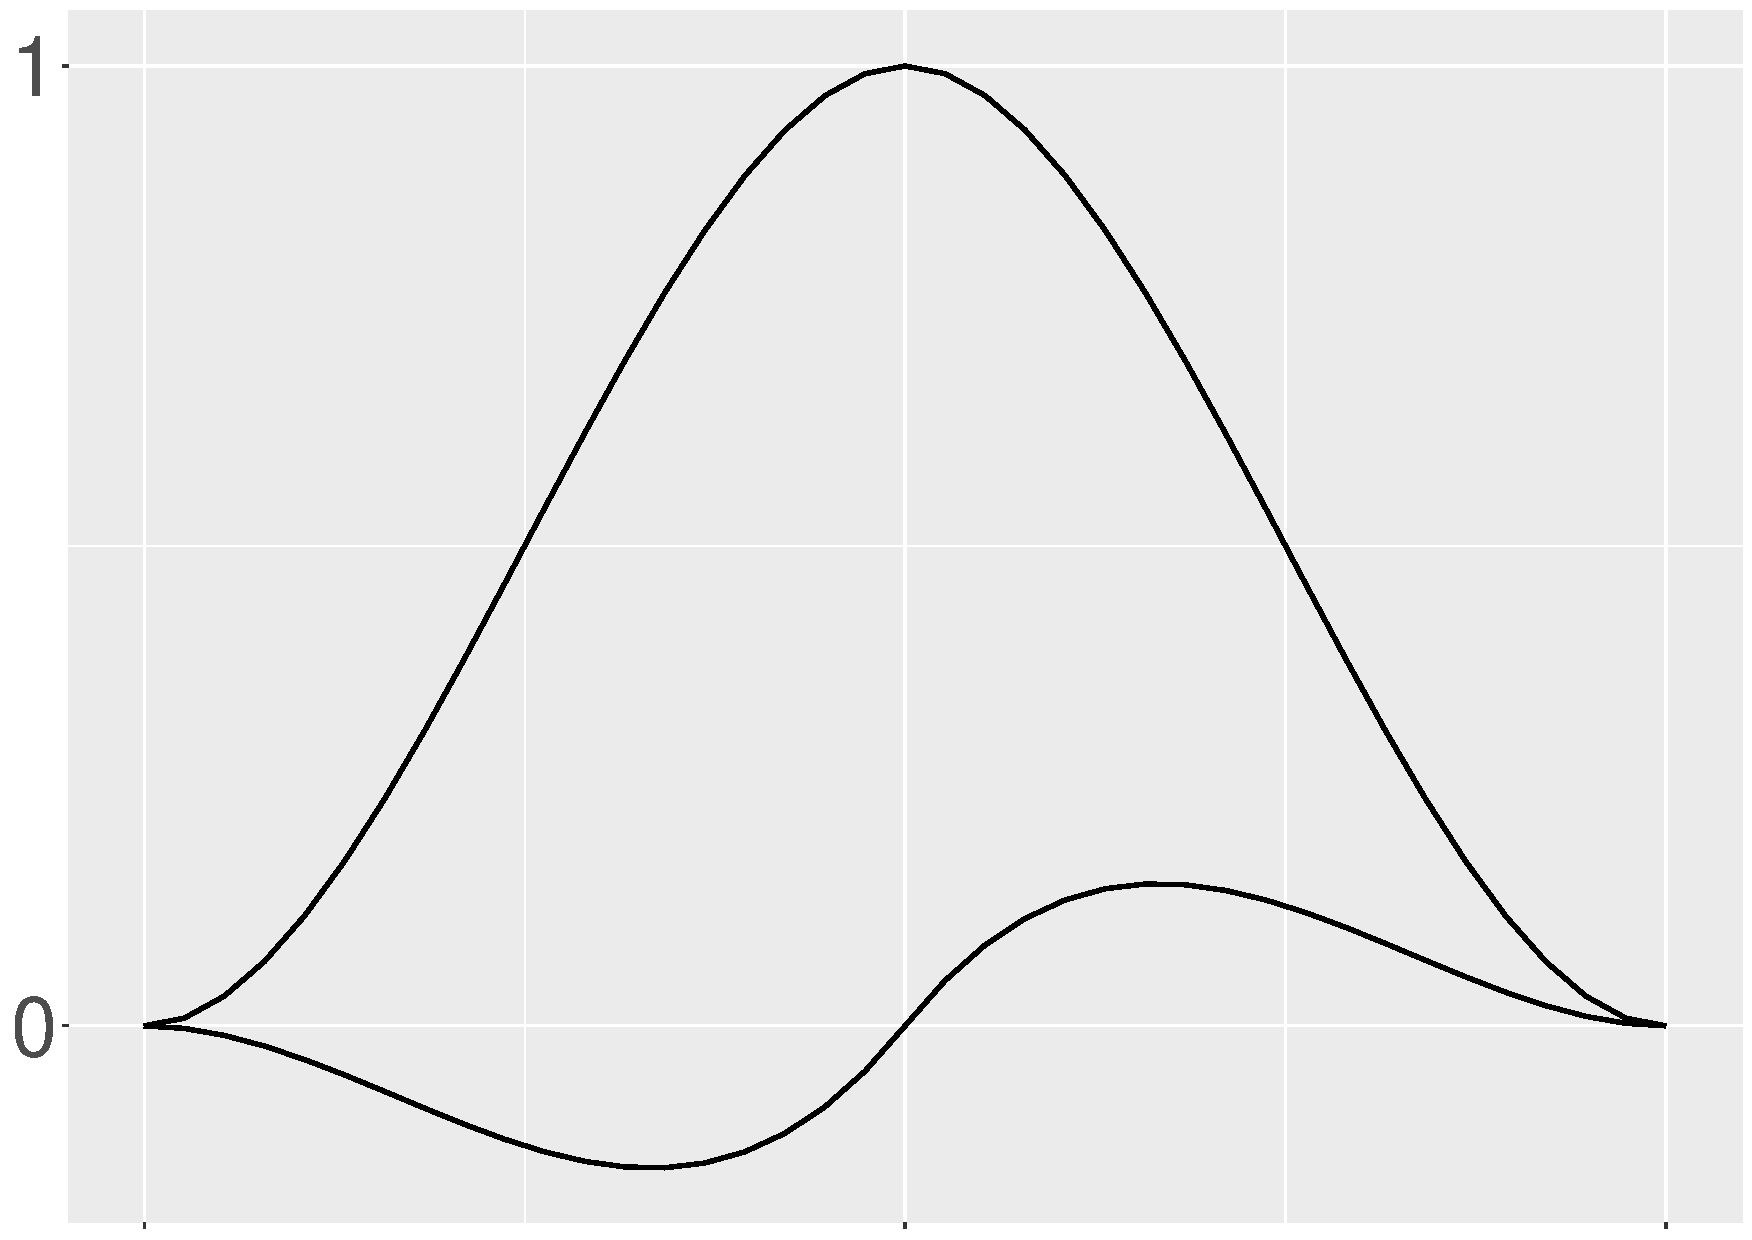
\includegraphics[width=0.7\textwidth,height=5cm]{Chapters/02TractorSplineTheory/plot/ggbasis.pdf}};
    \begin{scope}[
        x={(image.south east)},
        y={(image.north west)}
    ]
    \node [black, font=\bfseries] at (0.08,-0.02) {$t_i$};
    \node [black, font=\bfseries] at (0.52,-0.02) {$t_{i+1}$};
    \node [black, font=\bfseries] at (0.95,-0.02) {$t_{i+2}$};
    \end{scope}
\end{tikzpicture}
\caption{The two basis functions $N_{2i+1}$ (upper) and $N_{2i+2}$ (lower) on an arbitrary interval $[t_i, t_{i+2})$. Apparently, the basis functions are continuous on the interval and have continuous first derivatives.}\label{basisfigure}
\end{figure}

From the definition of basis functions, it can be seen that at a joint knot of two neighbor intervals, Hermite spline basis functions share the same $y_i$ and $v_i$. With this property, we construct V-spline basis functions. There are two parameters at each joint knots and 4 at the start and end knots. Hence, the degrees of freedom for parameters is $2n-4+4=2n$. However $2(n-2)$ constraints are added to the joint knots, at which the spline have continuous first and second derivatives. Additional two constraints are added to the starting and ending knots to keep their first derivatives continuous. Consequently, parameters' the degrees of freedom is 2. 


\subsection{Solution to The Objective Function}

Basis functions have been defined in the previous subsection, therefore the V-spline $f(t)$ on $[a,b]$, where $a \leq t_1 < t_2< \cdots < t_{n-1}<t_n \leq b$, can be found by minimizing  objective function \eqref{tractorsplineObjective}, which reduces to
\begin{equation}\label{tractormse}
\text{MSE}(\theta, \lambda,\gamma) = \left(\mathbf{y}-\mathbf{B}\theta\right)^\top \left(\mathbf{y}-\mathbf{B}\theta\right) +\gamma \left(\mathbf{v}-\mathbf{C}\theta\right)^\top \left(\mathbf{v}-\mathbf{C}\theta\right)+n \theta^\top\mathbf{\Omega}_{\lambda}\theta,
\end{equation}
where $\left\lbrace \mathbf{B}\right\rbrace_{ij} = N_j(t_i)$ , $\left\lbrace \mathbf{C}\right\rbrace_{ij} = N'_j(t_i)$ and $\left\lbrace \Omega_{2n}^{(i)} \right\rbrace_{jk}=\int_{t_i}^{t_{i+1}}\lambda_i N''_j(t)N''_k(t)dt$. After substituting the series observation $t_1, \ldots, t_n$ into basis functions, we get $N_1(t_1)=1, N_1(t_2)=0, \ldots, N_{2i-1}(t_{i})=1, N_{2i}(t_{i})=0, \ldots, N_{2n-1}(t_n)=1, N_{2n}(t_n)=0$; and into first derivative of basis functions, we get $N'_1(t_1)=0, N_1'(t_2)=1, \ldots, N_{2i-1}'(t_{i})=0, N_{2i}'(t_{i})=1, \ldots, N_{2n-1}'(t_n)=0, N_{2n}'(t_n)=1$. That means the matrices $\mathbf{B}$ and $\mathbf{C}$ in MSE equation \eqref{tractormse} are $n \times 2n$ dimensional and the elements are
\begin{align}
\mathbf{B}&=\left\lbrace B\right\rbrace_{ij}=\begin{cases}
1, & j=2i-1\\
0, & \mbox{otherwise}
\end{cases}\\
\mathbf{C}&=\left\lbrace C\right\rbrace_{ij}=\begin{cases}
1, & j=2i\\
0, & \mbox{otherwise}
\end{cases}
\end{align}
where $i=1, \ldots, n$, $j=1,\ldots,2n$ and $k=1,\ldots,2n$. The $i$-th $\Omega^{(i)}$ on the interval $[t_i,t_{i+1}]$ is a $2n \times 2n$ matrix and $\Omega^{(n)}$ does not exist. Its detail is in Appendix \ref{PenaltyTermDetails}. As a result, the penalty term is a bandwidth four matrix written in such a way:
\begin{equation}
\mathbf{\Omega}_\lambda=\sum_{i=1}^{n-1}\lambda_i\Omega^{(i)}.
\end{equation}



The solution to the equation \eqref{tractormse} is 
\begin{equation}\label{thetahat}
\hat{\theta}=\left(\mathbf{B}^\top\mathbf{B}+\gamma\mathbf{C}^\top\mathbf{C}+n\mathbf{\Omega}_{\lambda}\right)^{-1}\left(\mathbf{B}^\top\mathbf{y}+\gamma\mathbf{C}^\top\mathbf{v}\right)
\end{equation}
a generalized ridge regression. As a result, the fitted smoothing spline is given by
\begin{equation}
\hat{f}(t)=\sum_{k=1}^{2n}N_k(t)\hat{\theta}_k
\end{equation}

A smoothing spline with parameters $\lambda(t)$ and $\gamma$ is an example of a linear smoother \citep{esl2009}. This is because the estimated parameters in equation \eqref{thetahat} are a linear combination of $y_i$ and $v_i$. Denote by $\hat{\mathbf{f}}$ and $\hat{\mathbf{f}'}$ the $2n$ vector of fitted values $\hat{f}(t_i)$ and $\hat{f'}(t_i)$ at the training points $t_i$. Then
\begin{equation}
\begin{split}
\hat{\mathbf{f}} =&\mathbf{B}\left(\mathbf{B}^\top\mathbf{B}+\gamma\mathbf{C}^\top\mathbf{C}+n\mathbf{\Omega}_{\lambda}\right)^{-1}\left(\mathbf{B}^\top\mathbf{y}+\gamma\mathbf{C}^\top\mathbf{v}\right)\\
\triangleq & \mathbf{S}_{\lambda,\gamma}\mathbf{y}+\gamma\mathbf{T}_{\lambda,\gamma}\mathbf{v} 
\end{split}
\end{equation}
\begin{equation}
\begin{split}
\hat{\mathbf{f}'}
=&\mathbf{C}\left(\mathbf{B}^\top\mathbf{B}+\gamma\mathbf{C}^\top\mathbf{C}+n\mathbf{\Omega}_{\lambda}\right)^{-1}\left(\mathbf{B}^\top\mathbf{y}+\gamma\mathbf{C}^\top\mathbf{v}\right)\\
\triangleq&\mathbf{U}_{\lambda,\gamma}\mathbf{y}+\gamma\mathbf{V}_{\lambda,\gamma}\mathbf{v}
\end{split}
\end{equation}
The fitted $\hat{\mathbf{f}}$ and $\hat{\mathbf{f}'}$ are linear in $\mathbf{y}$ and $\mathbf{v}$, and the finite linear operators $\mathbf{S}_{\lambda,\gamma}, \mathbf{T}_{\lambda,\gamma}, \mathbf{U}_{\lambda,\gamma}$ and $\mathbf{V}_{\lambda,\gamma}$ are known as the smoother matrices. One consequence of this linearity is that the recipe for producing $\hat{\mathbf{f}}$ and $\hat{\mathbf{f}'}$ from $\mathbf{y}$ and $\mathbf{v}$, do not depend on $\mathbf{y}$ and $\mathbf{v}$ themselves; $\mathbf{S}_{\lambda,\gamma}, \mathbf{T}_{\lambda,\gamma}, \mathbf{U}_{\lambda,\gamma}$ and $\mathbf{V}_{\lambda,\gamma}$ depend only on $t_i,\lambda(t)$ and $\gamma$.

Suppose in a traditional least squares fitting, $\mathbf{B}_\xi$ is $N \times M$ matrix of $M$ cubic-spline basis functions evaluated at the $N$ training points $x_i$, with knot sequence $\xi$ and $M \ll N$. Thus the vector of fitted spline values is given by
\begin{align}\label{fhy}
\hat{\mathbf{f}}=\mathbf{B}_\xi\left(\mathbf{B}^\top_\xi\mathbf{B}_\xi\right)^{-1}\mathbf{B}_\xi\mathbf{y}=\mathbf{H}_\xi\mathbf{y}
\end{align}
Here the linear operator $\mathbf{H}_\xi$ is a symmetric, positive semidefinite matrices, and $\mathbf{H}_\xi\mathbf{H}_\xi=\mathbf{H}_\xi$ (idempotent) \citep{esl2009}. In our case, it is easily seen that $\mathbf{S}_{\lambda,\gamma}, \mathbf{T}_{\lambda,\gamma}, \mathbf{U}_{\lambda,\gamma}$ and $\mathbf{V}_{\lambda,\gamma}$ are symmetric, positive semidefinite matrices as well. Additionally, by Cholesky decomposition
\begin{equation}
\left(\mathbf{B}^\top\mathbf{B}+\gamma\mathbf{C}^\top\mathbf{C}+n\mathbf{\Omega}_{\lambda}\right)^{-1}=\mathbf{R}\mathbf{R}^\top,
\end{equation}
it is easy to prove that $\mathbf{T}_{\lambda,\gamma}=\mathbf{B}\mathbf{R}\mathbf{R}^\top\mathbf{C}^\top$ and $\mathbf{U}_{\lambda,\gamma}=\mathbf{C}\mathbf{R}\mathbf{R}^\top\mathbf{B}^\top$, then we will have 
 $\mathbf{T}_{\lambda,\gamma}= \mathbf{U}_{\lambda,\gamma}^\top$. When $\lambda=\gamma=0$, the matrix $\mathbf{S}_{\lambda_0,\gamma_0}=\mathbf{B}\left(\mathbf{B}^\top\mathbf{B}\right)^{-1}\mathbf{B}^\top$ is idempotent.  


\begin{corollary}\label{TractorsplineCorollary}
If $f(t)$ is the V-spline on the entire interval $[t_1,t_n]$, for sufficient cases of $\lambda(t)$ and $\gamma$, $f(t)$ has the following property:
\begin{enumerate}\itemsep0em 
\item if $\lambda(t)$ is piecewise constant and $\gamma \neq 0$, then $f$ and $f'$ are continuous, $f''$ is piecewise linear but not continuous at knots;
\item if $\lambda(t)$ is piecewise constant and $\gamma = 0$, the same as above;
\item if $\lambda(t)=\lambda $ is constant on the entire interval and $\gamma \neq 0$, the same as above;
\item if $\lambda(t)=\lambda $ is constant on the entire interval and $\gamma = 0$, then $f$, $f'$ are continuous, $f''$ is piecewise linear and continuous at knots.
\end{enumerate}
\end{corollary}

The proof of Corollary \ref{TractorsplineCorollary} is in Appendix \ref{proofofCorollary}. 

%Then we take some sample knots $\mathbf{y}^{(new)}$ with the same size of $\mathbf{y}$ from $\hat{\mathbf{f}}$ and reconstruct the spline function. It is easily seen that
% \begin{equation}
%\hat{\mathbf{f}}^{(new)} = \mathbf{S}_{\lambda_0,\gamma_0}\mathbf{y}^{(new)}=\mathbf{S}_{\lambda_0,\gamma_0}\mathbf{S}_{\lambda_0,\gamma_0}\mathbf{y}=(\mathbf{B}(\mathbf{B}^\top\mathbf{B})^{-1}\mathbf{B}^\top)(\mathbf{B}(\mathbf{B}^\top\mathbf{B})^{-1}\mathbf{B}^\top)=\mathbf{S}_{\lambda_0,\gamma_0}\mathbf{y},
 %\end{equation}
 %which returns the same reconstruction. So $\hat{\mathbf{f}}$ is generated and only affected by $\mathbf{y}$. And the same as $\hat{\mathbf{f}'}$, because
%\begin{equation}
%\hat{\mathbf{f}'}^{(new)}=\mathbf{U}_{\lambda_0,\gamma_0}\mathbf{y}^{(new)}=\mathbf{U}_{\lambda_0,\gamma_0}\mathbf{S}_{\lambda_0,\gamma_0}\mathbf{y}=(\mathbf{C}\mathbf{B} (\mathbf{B}^\top\mathbf{B})^{-1}\mathbf{B}^\top)(\mathbf{B}(\mathbf{B}^\top\mathbf{B})^{-1}\mathbf{B}^\top)\mathbf{y}=\mathbf{U}_{\lambda_0,\gamma_0}\mathbf{y}.
%\end{equation}
 %That means no matter how many times we reconstruct V-spline, once the matrices are fixed and observed knots are given, it will always return the same results when $\lambda=\gamma=0$.

%\begin{theorem}
%For $n\geq 2$, the objective function $J[f]$ in equation \eqref{tractorsplineObjective} is minimized by a V-spline.
%\end{theorem}



\subsection{Adjusted Penalty Term and Parameter Function}

To get the reconstructed trajectory in a multi-dimensional space, one can use the V-spline to find the trajectory in each dimension separately and then combine them together for a higher dimension, such as 2D and 3D. Typically, the data are not regularly sampled in time. Due to the property of Hermite spline, the combination of a multi-dimensional reconstruction for irregular time difference dataset will bring some issues.  Image the situation that a vehicle is moving along the $x$-axis, but stays unchanged on its $y$ position. By fitting $\mathbf{x}$ and $\mathbf{u}$, the V-spline $f_x(t)$ will give us the best fit which returns smallest errors to the objective function. While with the same parameter $\lambda(t)$ and $\gamma$, $f_y(t)$ returns a cubic curve, where it should give us a straight line as we expected. Moreover, in some circumstances, with time increasing $\mathbf{f}$ and $\mathbf{f}'$ remain the same, or change slightly. In this situation, the Hermite spline will return wiggles in each dimension and curves in combined two dimensions. 

To get a reliable reconstruction, we introduce an adjusted penalty term $\frac{\left(\Delta t_i\right)^\alpha}{\left(\Delta d_i\right)^\beta}$, where $\alpha \ge 0$ and $\beta \ge 0$, to the penalty function $\lambda(t)$, in which the V-spline is penalized by its real difference of $\Delta d_i$ and $\Delta t_i$ for each interval $[t_i, t_{i+1}]$. With this term, when either $\mathbf{u}$ for $x$ or $\mathbf{v}$ for $y$ goes down or equals to 0, it will make sure that the penalty function will be large enough and returns a straight line rather than a curve on this domain. Because of the unit of the penalty term is $m^2/t^3$, to keep the same scale, $\alpha$ and $\beta$ in the adjusted penalty term are chosen as $3$ and $2$ respectively. From the physical point of view, the term is the reciprocal of the product of velocity and acceleration. Either velocity or acceleration goes to zero, the moving object should either stop, which returns a straight line through time on $x$ or $y$ axes and a dot on the higher dimension or keep moving with the same speed, which returns a linear instead of a curved path. 

Thus, the final form of the penalty function is 
\begin{equation}\label{adjustedpenalty}
\lambda(t)=\frac{\left(\Delta t_i\right)^3}{\left(\Delta d_i\right)^2}\lambda,
\end{equation}
where  $t_i\leq t < t_{i+1}$. Eventually, in the objective function, there is one parameter $\lambda$ controlling the curvature of V-spline on different domains, and another one $\gamma$ controlling the residuals of velocity. 




\section{Parameter Selection and Cross-Validation}

The problem of choosing the smoothing parameter is ubiquitous in curve estimation, and there are two different philosophical approaches to this question. The first one is to regard the free choice of smoothing parameter as an advantageous feature of the procedure. The other one is to find the parameter automatically by the data \citep{green1993nonparametric}. We prefer the latter one, use data to train our model and find the best parameters. The most well-known method is cross-validation.


Assuming that mean of the random errors is zero, the true regression curve $f(t)$ has the property that, if an observation $y$ is taken away at a point $t$, the value $f(t)$ is the best predictor of $y$ in terms of returning a least value of $\left(y-f(t)\right)^2$. 

Now, focus on an observation $y_i$ at point $t_i$ as being a new observation by omitting it from the set of data, which are used to estimate $\hat{f}$. Denote by $\hat{f}^{(-i)}(t,\lambda)$ the estimated function from the remaining data, where $\lambda$ is the smoothing parameter. Then $\hat{f}^{(-i)}\left(t,\lambda\right)$ is the minimizer of  
\begin{equation}\label{originalcv}
\frac{1}{n}\sum_{j \neq i}\left(y_j-f(t_j) \right)^2+\lambda\int (f'')^2dt,
\end{equation}
and can be quantified by the cross-validation score function
\begin{equation*}
\mbox{CV}(\lambda)=\frac{1}{n}\sum_{i=1}^{n}\left(  y_i-\hat{f}^{(-i)}(t_i,\lambda)\right) ^2.
\end{equation*}
The basis idea of the cross-validation is to choose the value of $\lambda$ that minimizes $\mbox{CV}(\lambda)$ \citep{green1993nonparametric}. 

%An efficient way to calculate the cross-validation score is introduced by \citep{green1993nonparametric}. 
Through the equation \eqref{fhy}, it is known that the value of the smoothing spline $\hat{f}$ depend linearly on the data $y_i$. Define the matrix $A(\lambda)$, which is a map vector of observed values $y_i$ to predicted values $\hat{f}(t_i)$. Then we have
\begin{equation*}\label{crossvalidationmatrixA}
\hat{\mathbf{f}}=A(\lambda)\mathbf{y}
\end{equation*}
and the following lemma.
\begin{lemma}\label{cvlema}
The cross-validation score satisfies
\begin{equation*}
\mbox{CV}(\lambda)=\frac{1}{n} \sum_{i=1}^n \left(\frac{y_i-\hat{f}(t_i)}{1-A_{ii}(\lambda)}\right)^2
\end{equation*}
where $\hat{f}$ is the spline smoother calculated from the full data set $\left\lbrace (t_i,y_i)\right\rbrace$ with smoothing parameter $\lambda$.
\end{lemma}

For a V-spline and its MSE function, there are two parameters $\lambda(t)$ and $\gamma$ to be estimated for. Therefore, $\hat{f}^{(-i)}(t,\lambda)$ is the minimizer of  
\begin{align}
\frac{1}{n}\sum_{j \neq i}\left( y_j-f(t_j) \right)^2+\frac{\gamma}{n}\sum_{j \neq i} \left( v_j-f'(t_j) \right)^2+ \int \lambda(t) \left( f'' \right)^2dt,
\end{align}
and the cross-validation score function is
\begin{align}
\mbox{CV}\left(\lambda(t),\gamma\right)=\frac{1}{n}\sum_{i=1}^{n}\left( y_i-\hat{f}^{(-i)}\left(t_i,\lambda(t),\gamma\right) \right) ^2.
\end{align}
Additionally, it is known that the parameter $\hat{\theta}=\left(B^\top B+\gamma C^\top C+n\Omega_\lambda\right)^{-1}\left(B^\top\mathbf{y}+\gamma C^\top\mathbf{v}\right)$ and will give us the following form \small
\begin{equation}
\begin{split}
 \hat{\mathbf{f}}&=B\hat{\theta}=B\left(B^\top B+\gamma C^\top C+n\Omega_\lambda\right)^{-1}B^\top\mathbf{y}+B\left(B^\top B+\gamma C^\top C+n\Omega_\lambda\right)^{-1} C^\top\mathbf{v}\\&=S\mathbf{y}+\gamma T\mathbf{v},
 \end{split}
 \end{equation}
 \begin{equation}
 \begin{split}
\hat{\mathbf{f}}'&=C\hat{\theta}=C\left(B^\top B+\gamma C^\top C+n\Omega_\lambda\right)^{-1}B^\top\mathbf{y}+C\left(B^\top B+\gamma C^\top C+n\Omega_\lambda\right)^{-1}C^\top \mathbf{v}\\&=U\mathbf{y}+\gamma V\mathbf{v}.
 \end{split}
\end{equation}\normalsize
From Lemma \ref{cvlema}, we can prove the following theorem: 
\begin{theorem}\label{tractorsplinecvscore}
The cross-validation score of a V-spline satisfies
\begin{equation}\label{tractorcv}
\mbox{CV}\left(\lambda(t),\gamma\right)=\frac{1}{n}\sum_{i=1}^{n} \left( \frac{\hat{f}(t_i)-y_i+\gamma \frac{T_{ii}}{1-\gamma V_{ii}}(\hat{f}'(t_i)-v_i)}{1-S_{ii}-\gamma\frac{T_{ii}}{1-\gamma V_{ii}}U_{ii}} \right)^2
\end{equation}
where $\hat{f}$ is the V-spline smoother calculated from the full data set $\left\lbrace (t_i,y_i,v_i)\right\rbrace$ with smoothing parameter $\lambda(t)$ and $\gamma$.
\end{theorem}

The proof of Theorem \ref{tractorsplinecvscore} follows immediately from a lemma, and gives an expression for the deleted residuals $y_i-\hat{f}^{(-i)}(t_i)$ and $v_i-\hat{f}'^{(-i)}(t_i)$ in terms of $y_i-\hat{f}(t_i)$ and $v_i-\hat{f}'(t_i)$ respectively. 

\begin{lemma} \label{cvlemma}
For fixed $\lambda(t),\gamma$ and $i$, denote $\mathbf{f}^{(-i)}$ by the vector with components $f_j^{(-i)}=\hat{f}^{(-i)}\left(t_j,\lambda(t),\gamma\right)$,  $\mathbf{f}'^{(-i)}$ by the vector with components $f_j'^{(-i)}=\hat{f}'^{(-i)}\left(t_j,\lambda(t),\gamma\right)$, and define vectors $\mathbf{y}^*$ and $\mathbf{v}^*$ by 
\begin{align}
\begin{cases}
y_j^*=y_j &j \neq i\\
y_i^*=\hat{f}^{(-i)}(t_i) &\mbox{otherwise}
\end{cases}\\
\begin{cases}
v_j^*=v_j &j \neq i\\
v_i^*=\hat{f}'^{(-i)}(t_i) &\mbox{otherwise}
\end{cases}
\end{align}
Then
\begin{align}
\mathbf{\hat{f}}^{(-i)}&=S\mathbf{y}^*+\gamma T\mathbf{v}^*\\
\mathbf{\hat{f}}'^{(-i)}&=U\mathbf{y}^*+\gamma V\mathbf{v}^*
\end{align}
\end{lemma}


\section{Simulation Study} %and Error Analysis}


\subsection{Numerical Examples}

In this section, we examine the visual quality of the proposed method with four functions: \textit{Blocks}, \textit{Bumps}, \textit{HeaviSine} and \textit{Doppler}, which have been used in \citep{donoho1994ideal, donoho1995adapting, abramovich1998wavelet} because of their caricature features in imaging, spectroscopy and other scientific signal processing. However it is unfair for V-spline fitting "jump" position in \textit{Blocks} and \textit{Bumps} function because it fits position and velocity simultaneously and these points imply infinite first derivative in original functions, which are impossible for vehicles or individuals. In terms of this issue, we treat these functions as velocity, and use noise free points to generate accurate position data, then add noises back to them.

For calculating consideration, we use $n=1024$ \citep{nason2010wavelet}. Because of all noises are randomly generated, for the convenience of reinitialization and repeatable comparison, we set random seed at 2016. The noises are \iid zero-mean Gaussian distributed with standard deviation regarding to signal-to-noise ratio (SNR), which specifies the ratio of the standard deviation of the function to the standard deviation of the simulated errors. Explicitly, if the standard deviation of the true signal $f$ is $\sigma_f$, the simulated data will be $f+\varepsilon$, where the simulated error  $\varepsilon \sim N(0,\sigma_f/SNR)$. 

If the original function $g(t)$ is treated as velocity function $f'(t)=g(t)$, thus by setting initial position $y_0=0$, acceleration $a_0=0$ and using the following formula 
\begin{equation}\label{generateVelocity}
f(t_{i+1})=f(t_i)+\left(g(t_i)+g(t_{i+1}) \right)\frac{t_{i+1}-t_i}{2}
\end{equation}
for calculating position information, we can generate simulated data. Further, we add some \iid  zero-mean $\varepsilon$ noises with SNR to them to get the measurements by 
\begin{align}\label{tractorsplinegeneratefunctions}
\begin{split}
y_i &= f(t_i) + \varepsilon_f, \\
v_i &= g(t_i) + \varepsilon_g,
\end{split}
\end{align}
where $\varepsilon_f\sim N(0,\sigma_f/SNR)$ and $\varepsilon_g\sim N(0,\sigma_g/SNR)$. The value of SNR can be chosen 7 or 3. For wavelet transform reconstructions, we use the threshold policy of \textit{sure} and \textit{BayesThresh} with levels $l=4, \ldots, 9$, see  \citep{donoho1995adapting, abramovich1998wavelet}. A semi-parametric regression model with spatially adaptive penalized splines (\textit{P-spline}) is added in comparison, see \citep{krivobokova2008fast, ruppert2003semiparametric}.

For V-spline, we have two parameters $\lambda$ and $\gamma$ to optimize. To evaluate the performance of the velocity term in objective function \eqref{tractorsplineObjective} and the adjusted penalty term in \eqref{adjustedpenalty}, the parameter $\gamma$ is set as 0 in one reconstruction of V-spline, whose objective function and solution become
\begin{equation}\label{ofgamma0}
J[f]_{\gamma=0}= \frac{1}{n} \sum_{i=1}^{n} \left(f(t_i)-y_i\right)^2 +\sum_{i=1}^{n-1} \lambda_i\int_{t_i}^{t_{i+1}} \left(f''\right)^2 dt,
\end{equation}
and
\begin{equation}\label{thetahat0}
\hat{\theta}_{\gamma=0}=\left(\mathbf{B}^\top\mathbf{B}+n\Omega_{\lambda}\right)^{-1}\mathbf{B}^\top\mathbf{y}
\end{equation}
and the adjusted penalty term in \eqref{adjustedpenalty} was removed from another reconstruction, noted as "V-spline without APT". Figure \ref{num1} to \ref{num4} display the original (velocity), generated position, wavelet with two different threshold methods, P-spline and three kinds of V-spline fitted functions. The parameters $\lambda$ and $\gamma$ of a V-spline are automatically selected with the formula \eqref{tractorcv} by $\textsf{optim}$ function in $R$ \citep{nelder1965simplex}.


%\begin{figure}
%  \centering
%   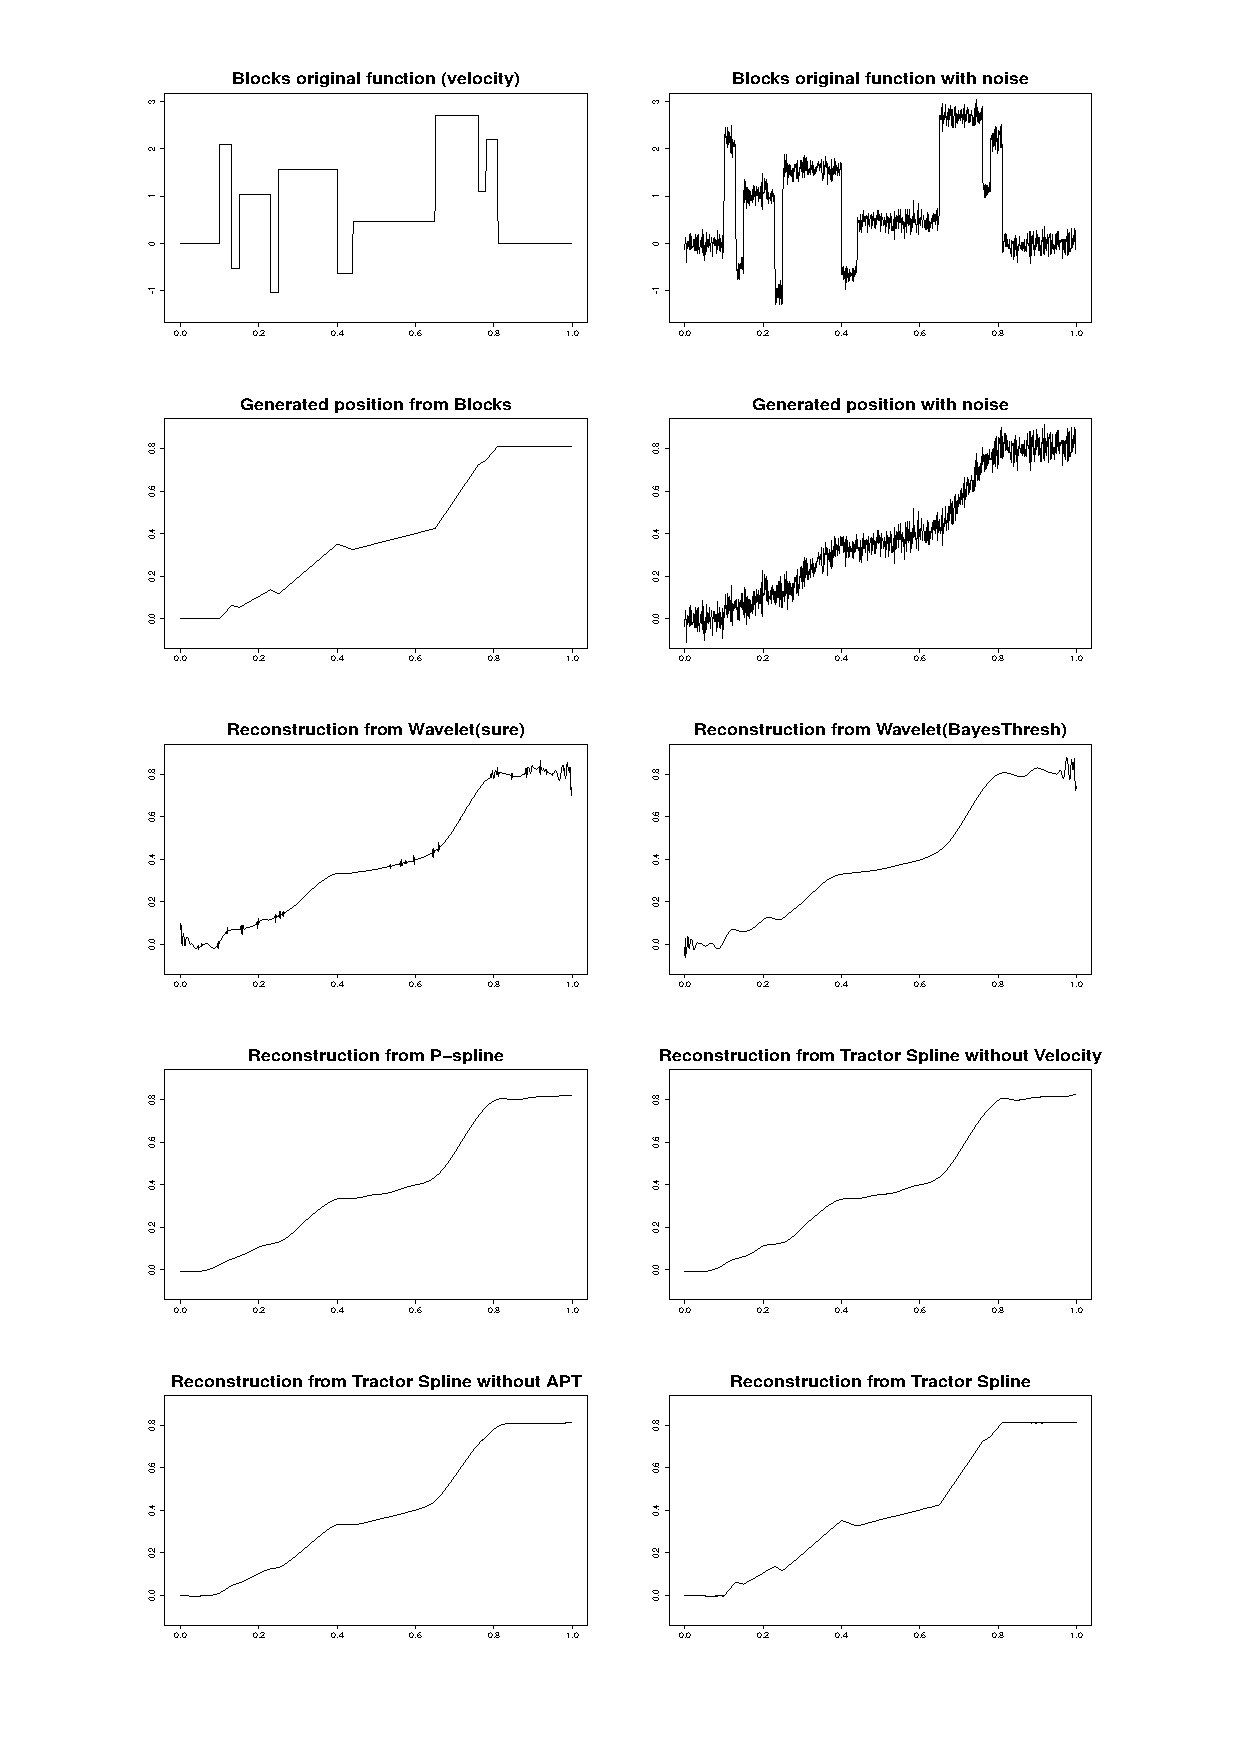
\includegraphics[width=\textwidth,height=14cm]{Chapters/02TractorSplineTheory/plot/blocks10} 
%  \caption{Numerical example: $\textit{Blocks}$. (a) The true velocity function. (b) Velocity with Gaussian noise at SNR=7. (c) Generated position function. (d) Position with Gaussian noise at SNR=7. (e) Reconstruction from Wavelet with sure threshold. (f) Reconstruction from Wavelet with BayesThresh approach. (g) Reconstruction by P-spline. (h) Reconstruction by V-spline setting $\gamma=0$. (i) Reconstruction by V-spline with normal penalty term. (j) Reconstruction by proposed V-spline.}\label{num1}
%\end{figure}

\begin{figure}
    \centering
    \begin{subfigure}{0.45\textwidth}
    \centering
    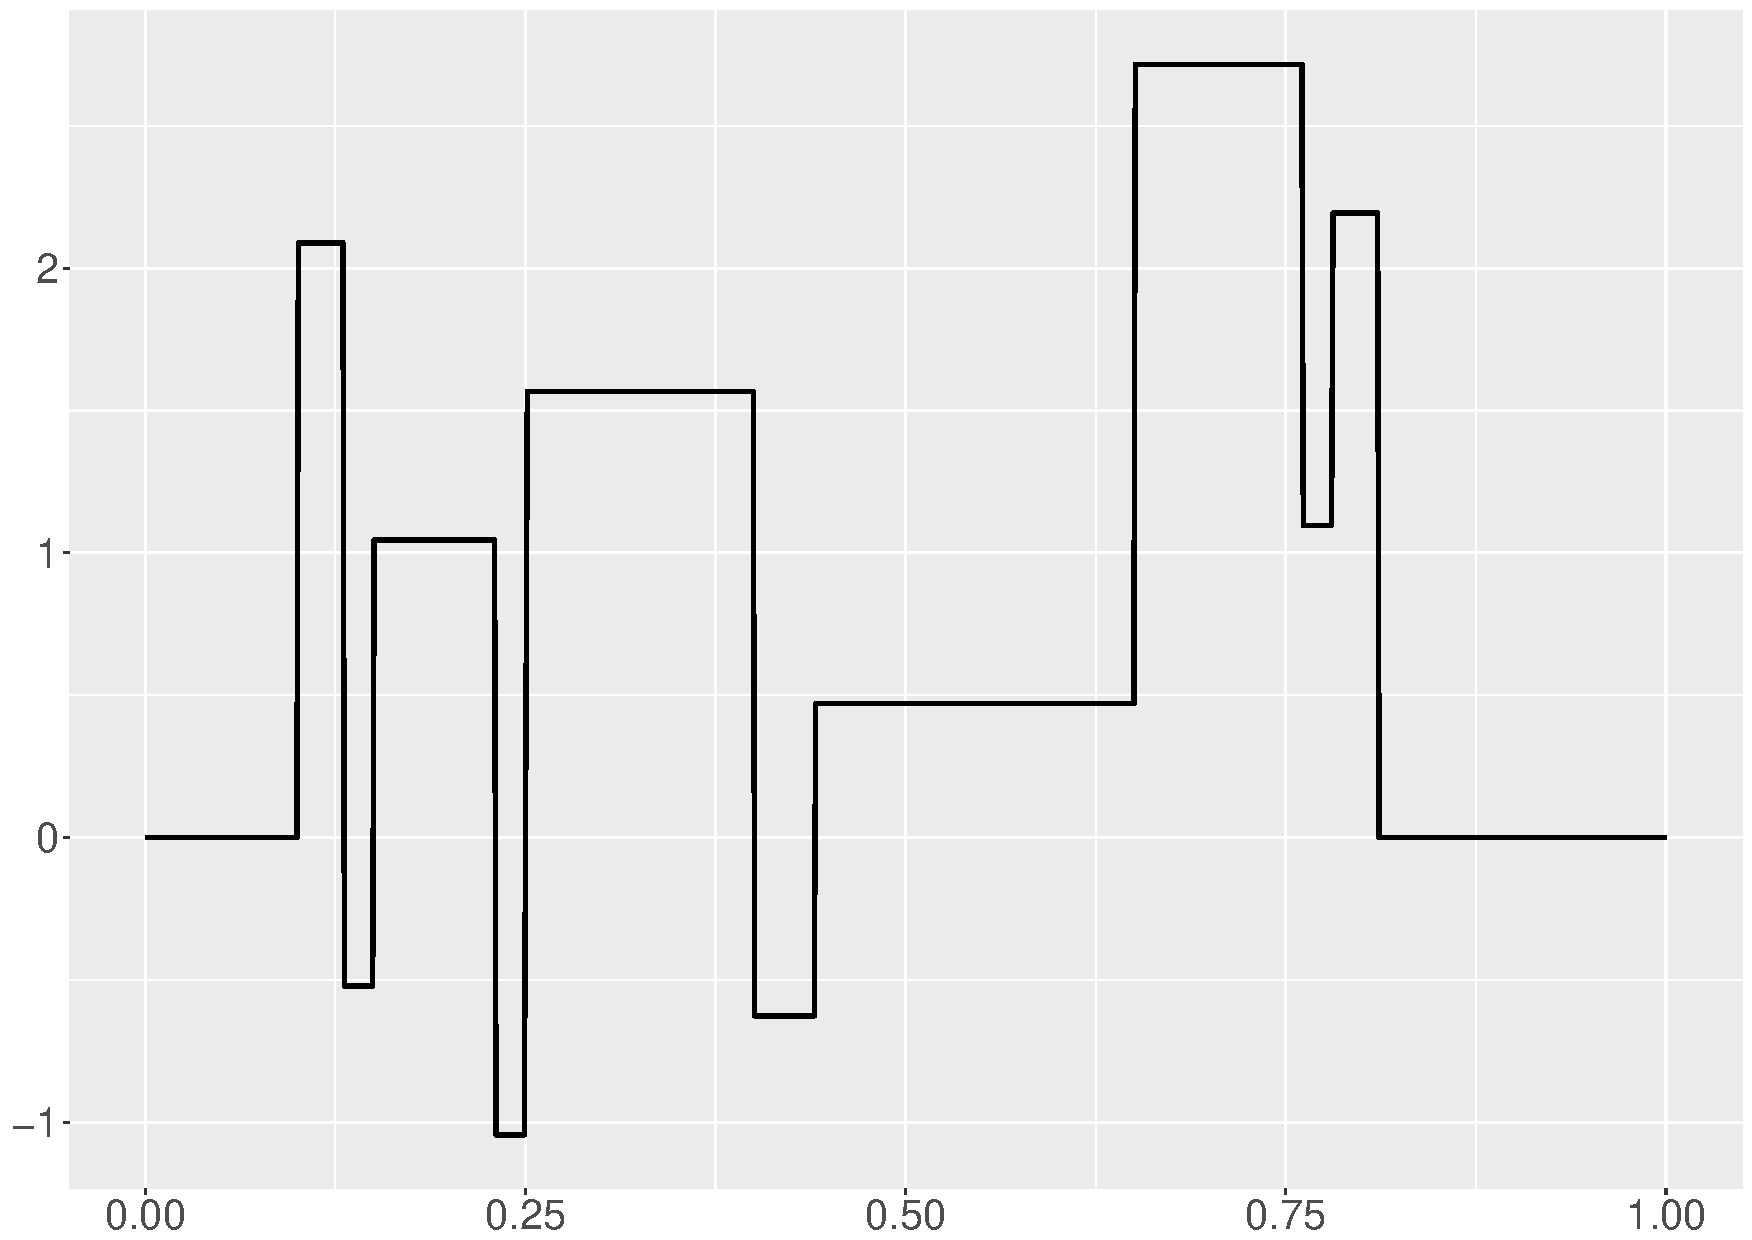
\includegraphics[width=\linewidth,height=0.45\textwidth]{Chapters/02TractorSplineTheory/plot/ggplot/ggBlocks.pdf}
    \caption{The \textit{Blocks} function}
    \end{subfigure}%
    \begin{subfigure}{0.45\textwidth}
    \centering
    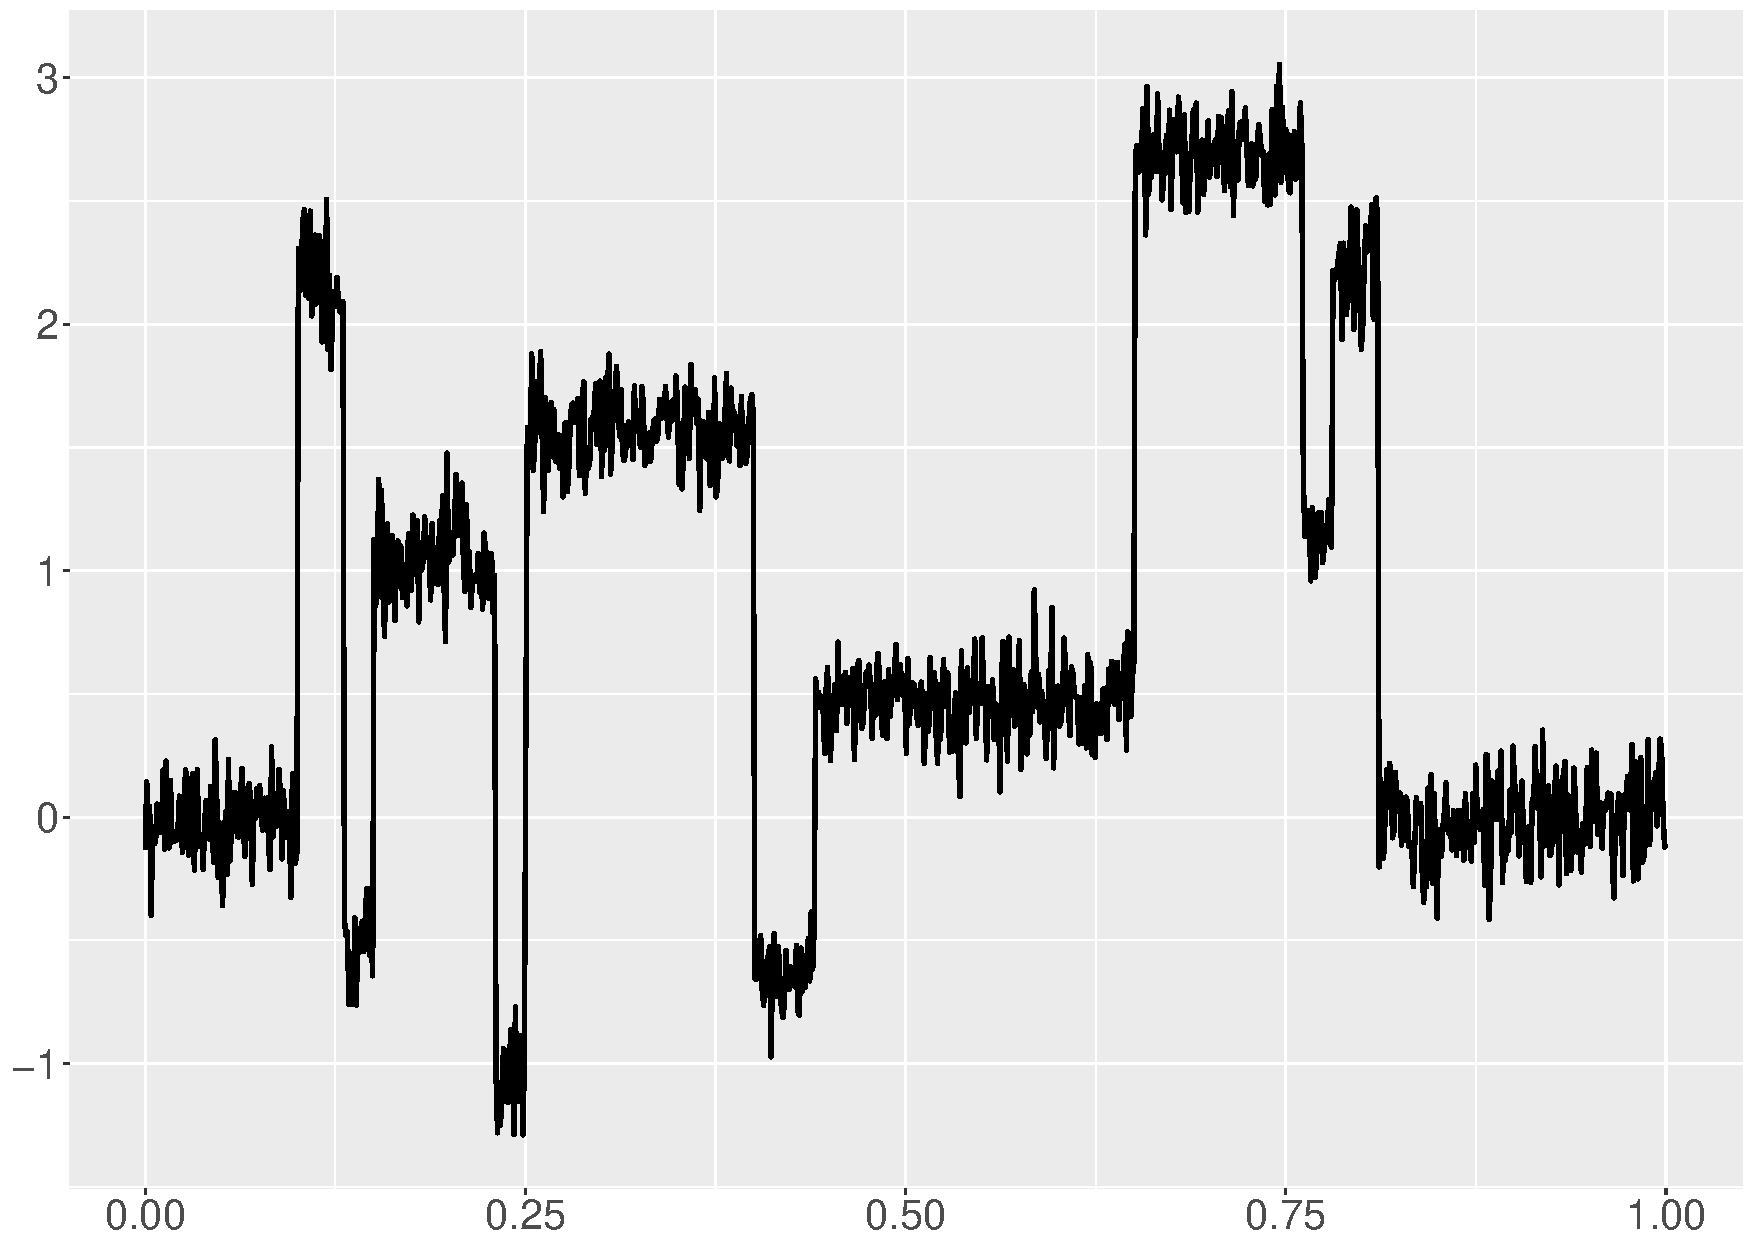
\includegraphics[width=\linewidth,,height=0.45\textwidth]{Chapters/02TractorSplineTheory/plot/ggplot/ggBlocksNoise.pdf}
    \caption{Noisy \textit{Blocks} at \textit{SNR}=7}
    \end{subfigure}
    \begin{subfigure}{0.45\textwidth}
    \centering
    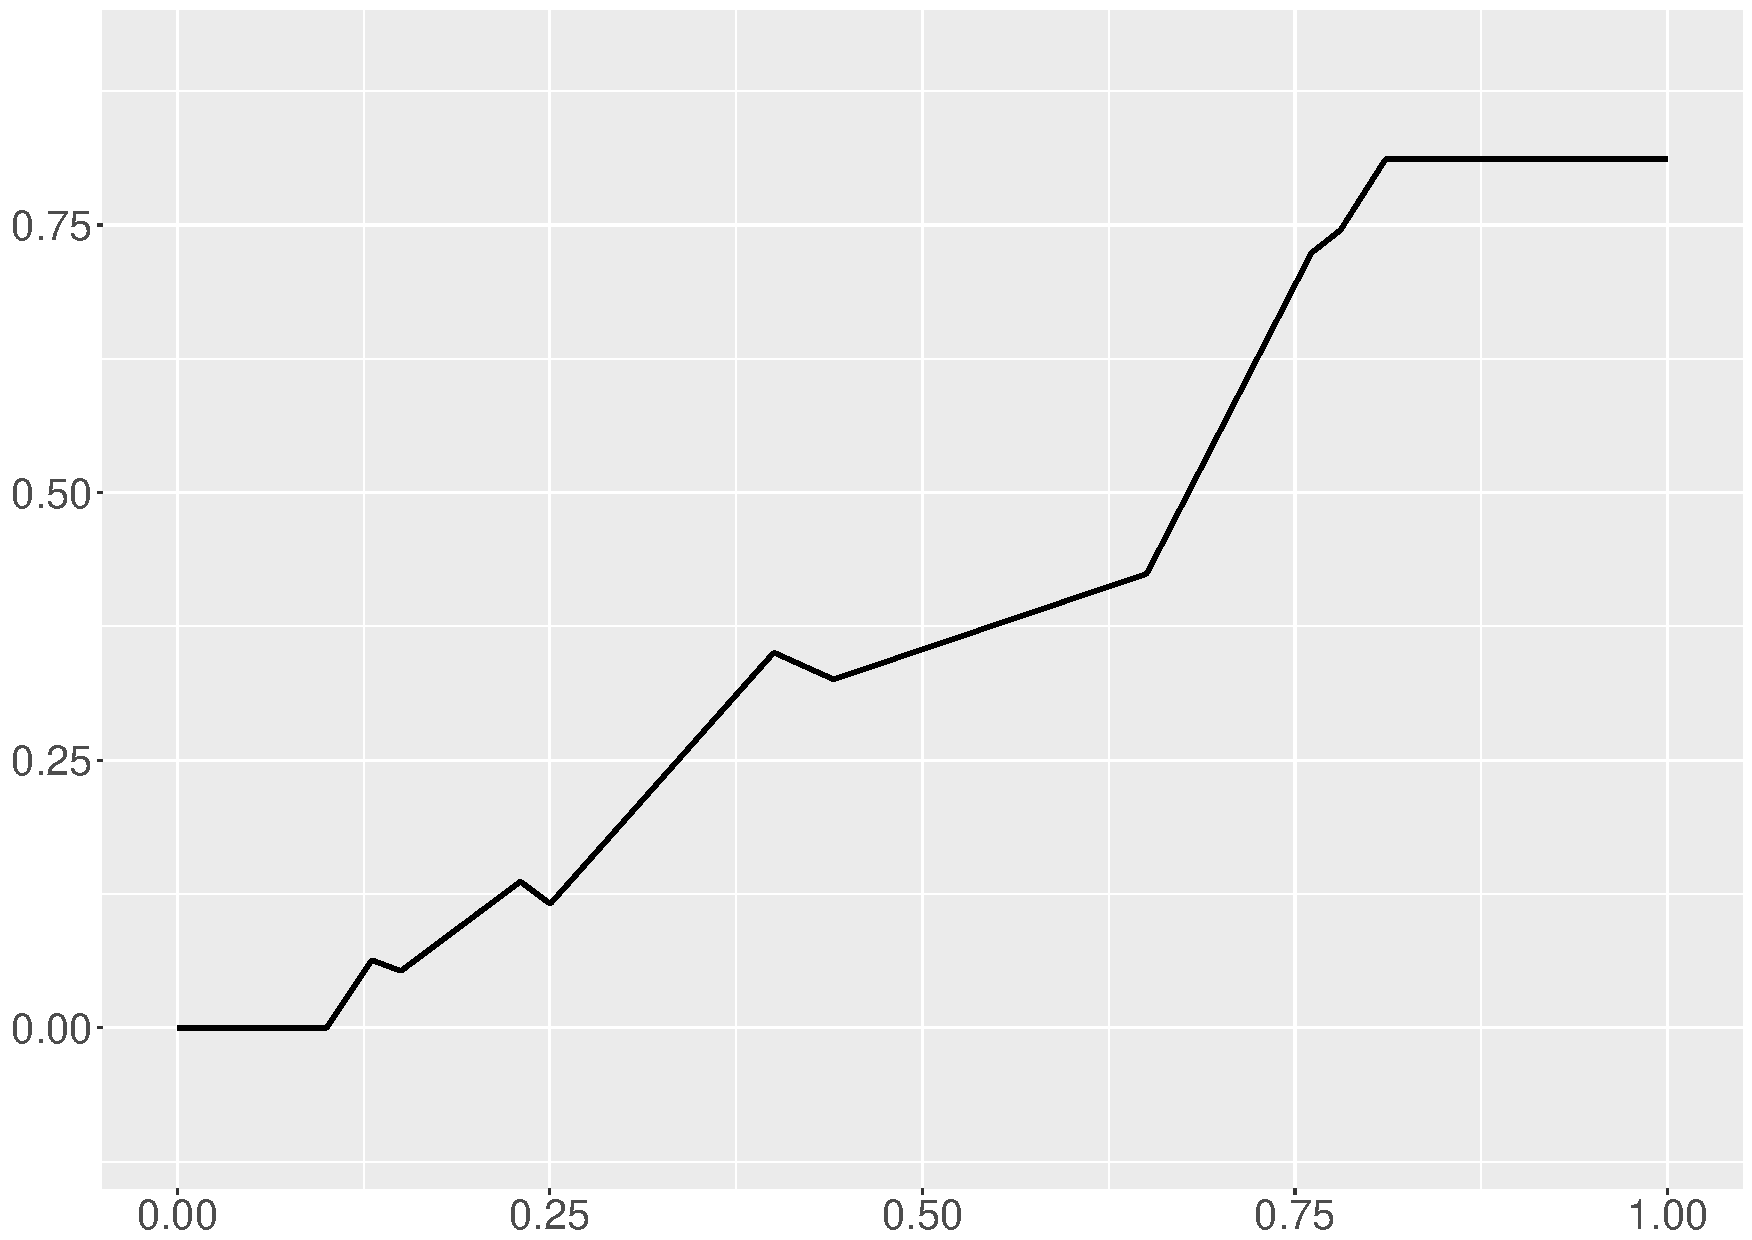
\includegraphics[width=\linewidth,height=0.45\textwidth]{Chapters/02TractorSplineTheory/plot/ggplot/ggBlocksPosition.pdf}
    \caption{Generated positions}
    \end{subfigure}
    \begin{subfigure}{0.45\textwidth}
    \centering
    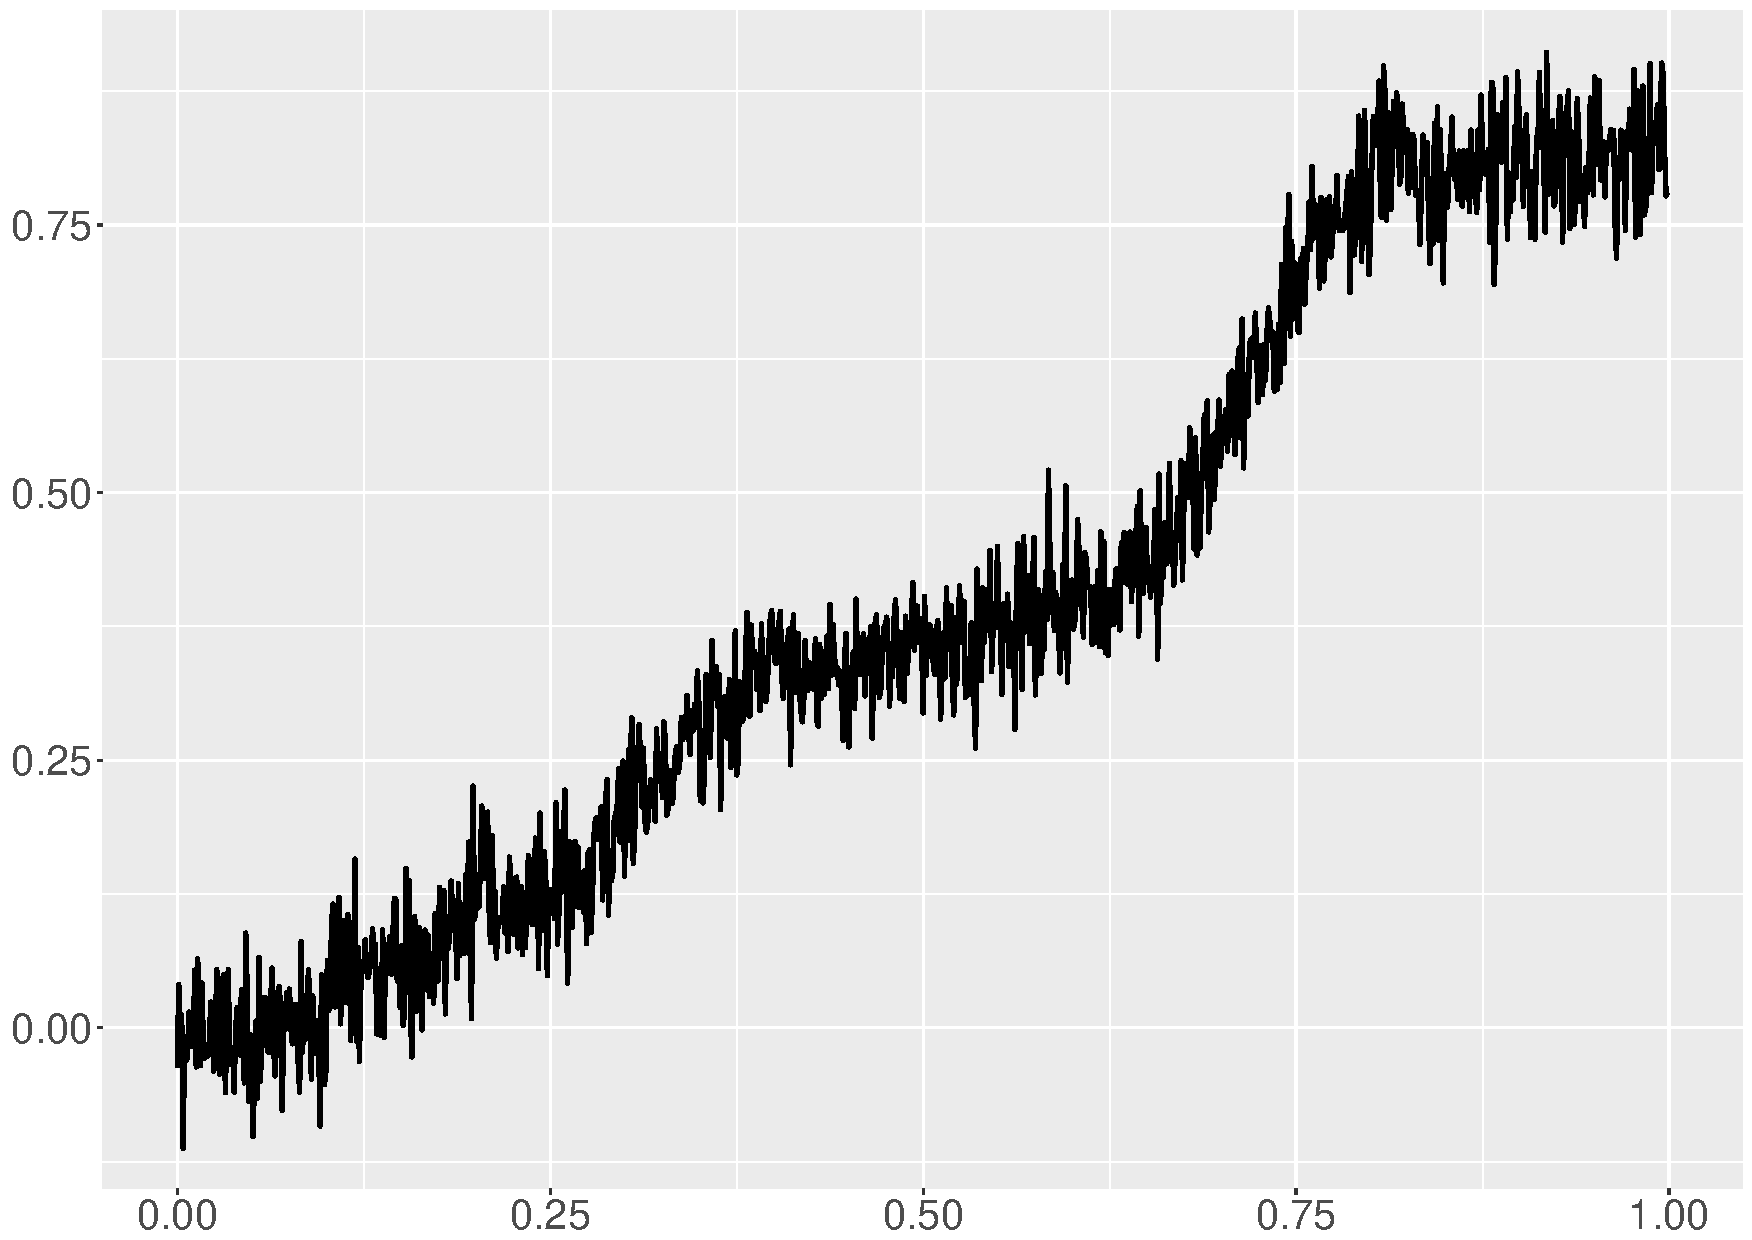
\includegraphics[width=\linewidth,height=0.45\textwidth]{Chapters/02TractorSplineTheory/plot/ggplot/ggBlocksPositionNoise.pdf}
    \caption{Noisy position at \textit{SNR}=7}
    \end{subfigure}
    \begin{subfigure}{0.45\textwidth}
    \centering
    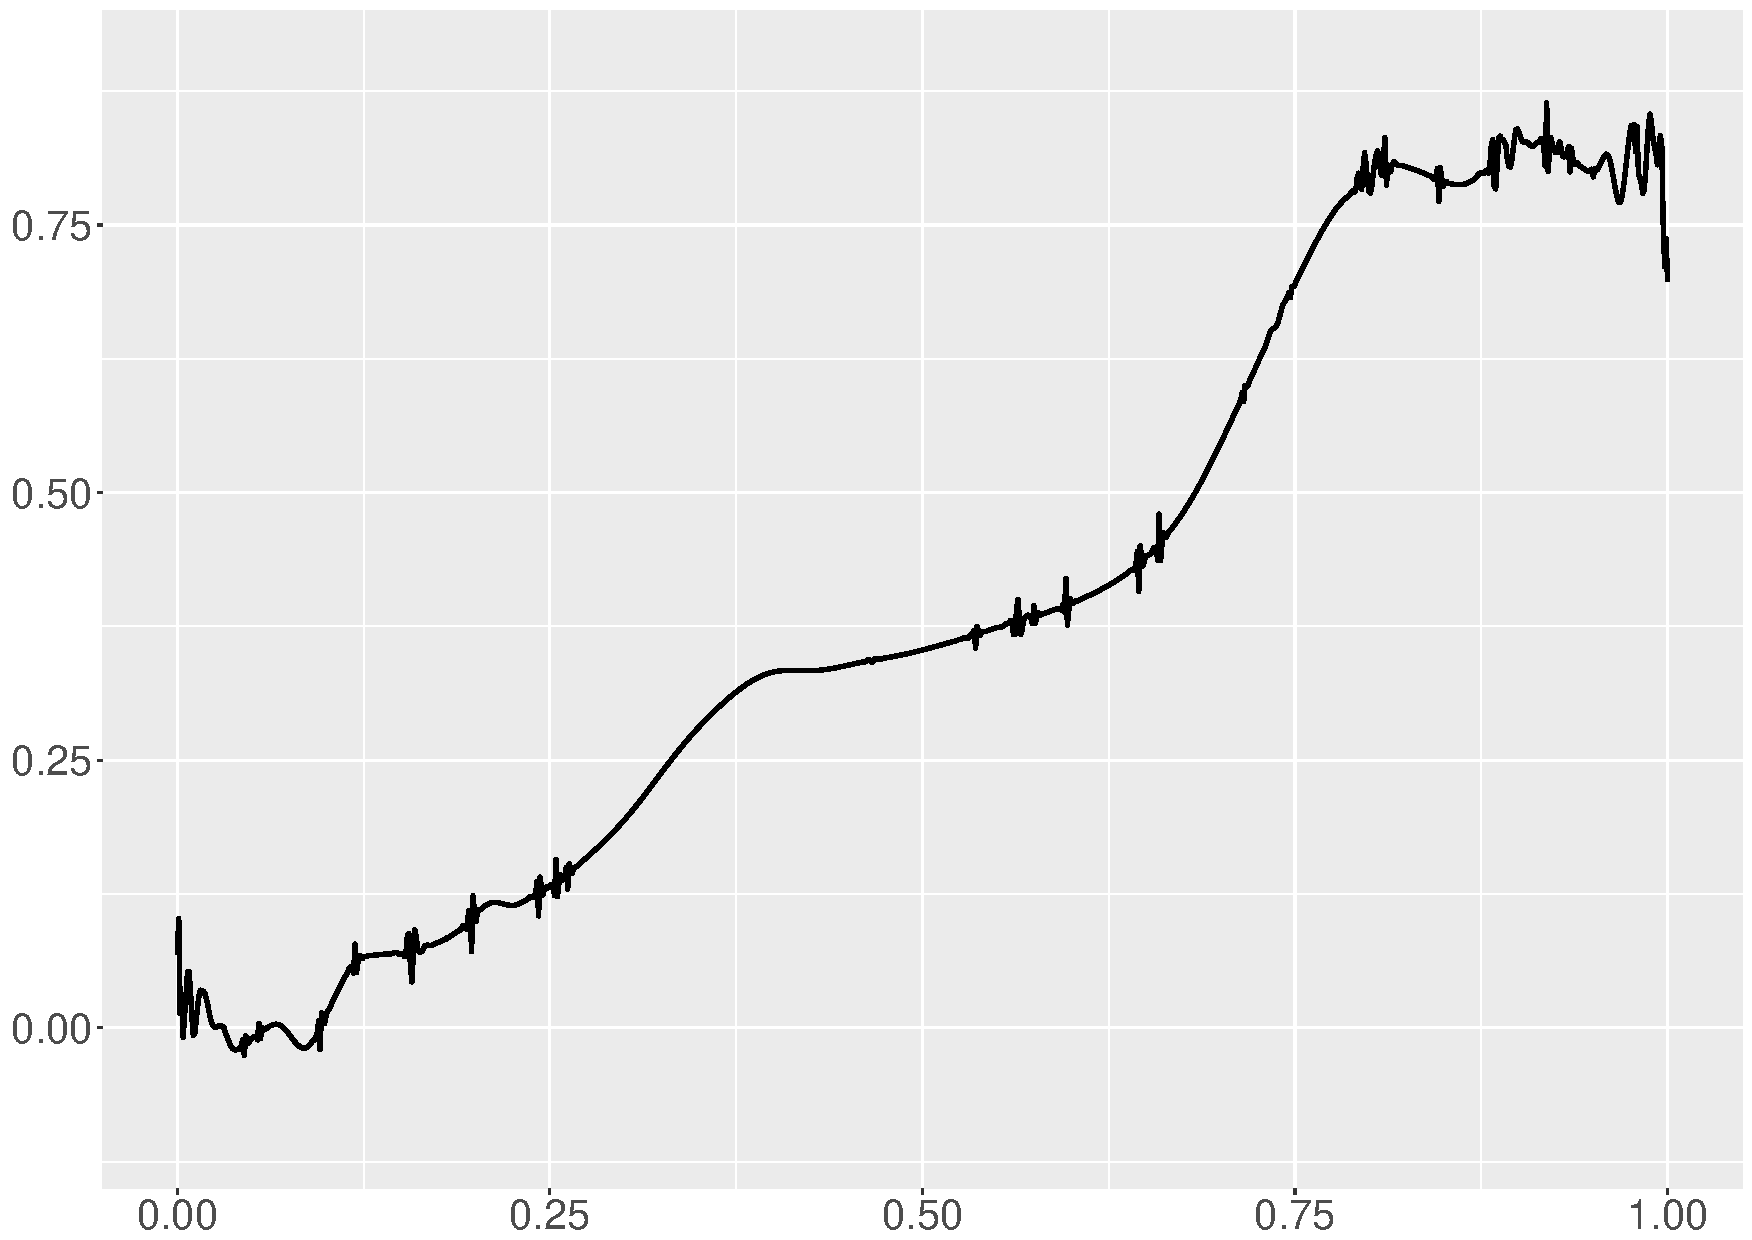
\includegraphics[width=\linewidth,height=0.45\textwidth]{Chapters/02TractorSplineTheory/plot/ggplot/ggBlocksSure.pdf}
    \caption{Reconstruction from Wavelet by sure threshold}
    \end{subfigure}
    \begin{subfigure}{0.45\textwidth}
    \centering
    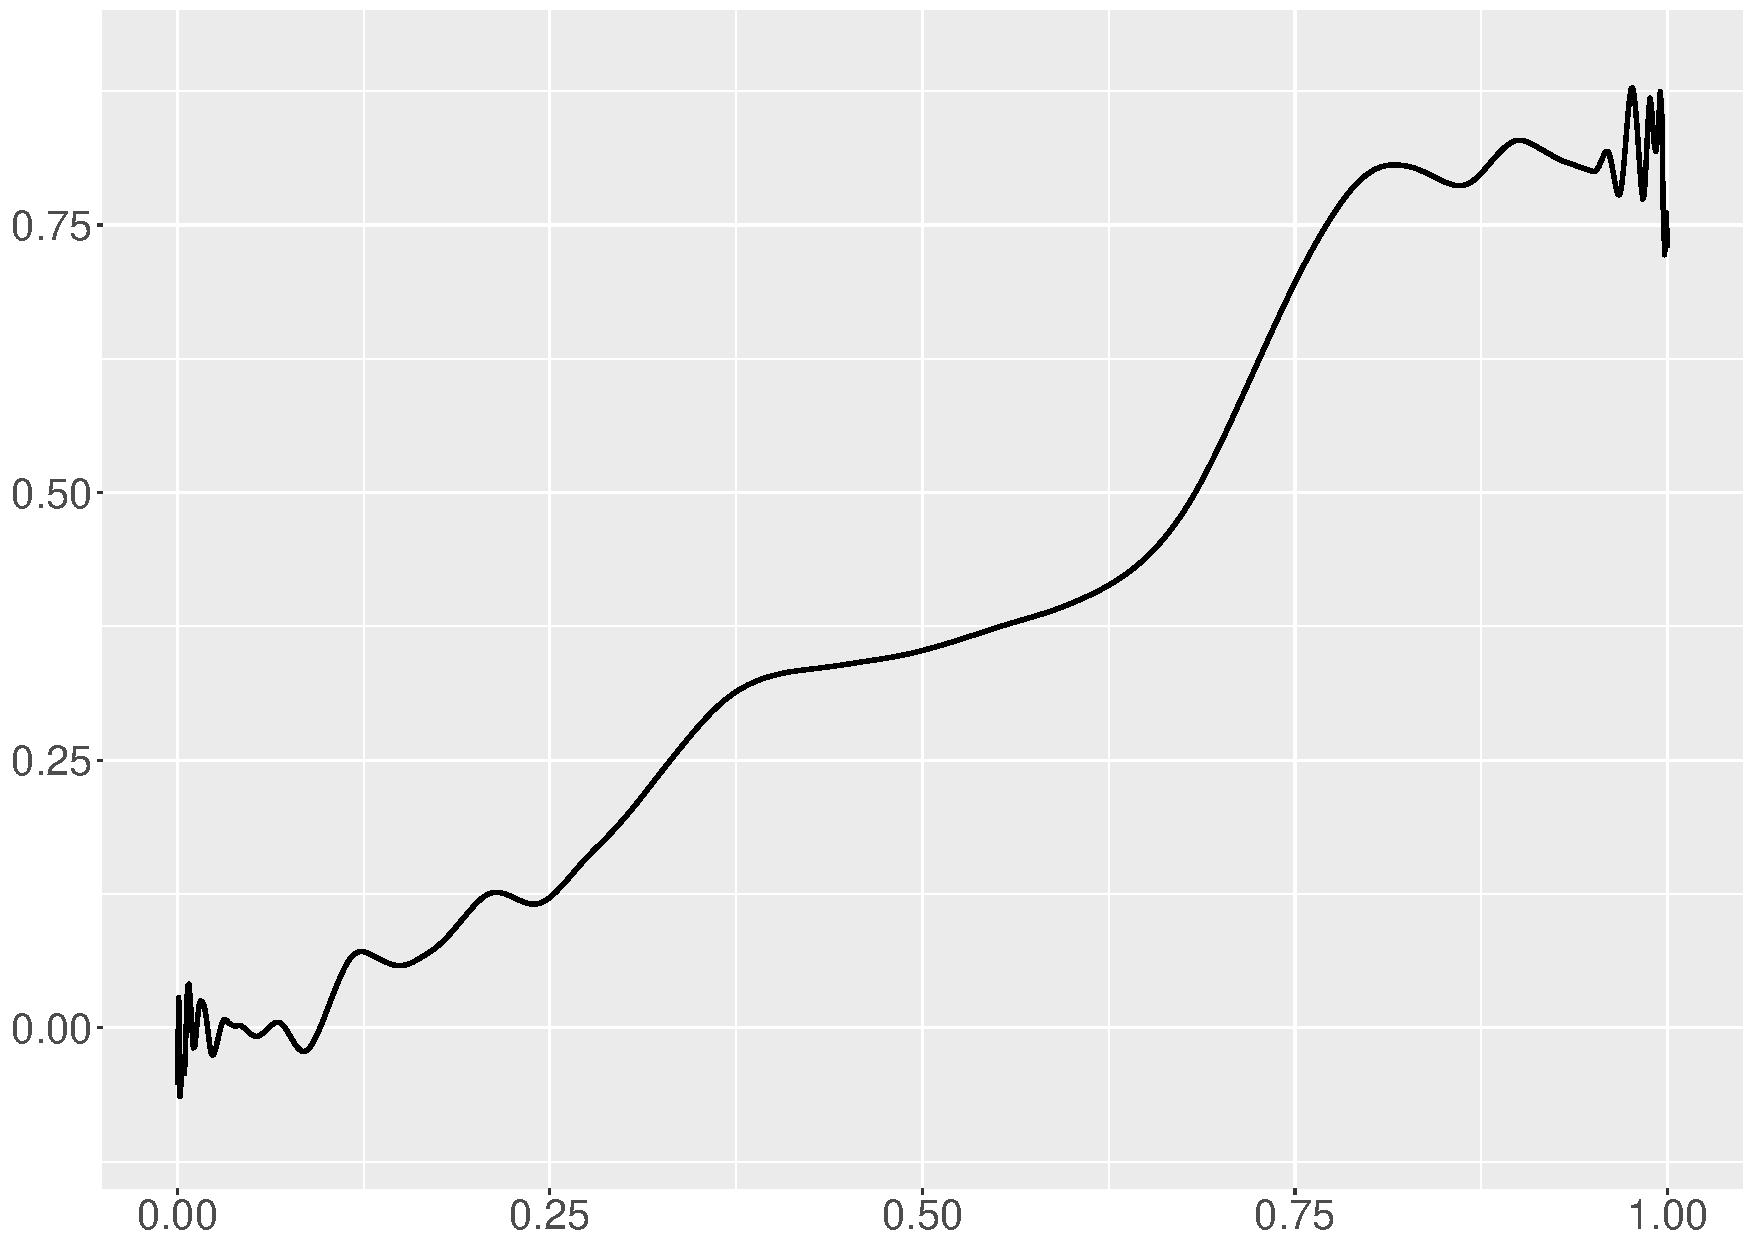
\includegraphics[width=\linewidth,height=0.45\textwidth]{Chapters/02TractorSplineTheory/plot/ggplot/ggBlocksBayes.pdf}
    \caption{Reconstruction from Wavelet by BayesThresh approach}
    \end{subfigure}
    \begin{subfigure}{0.45\textwidth}
    \centering
    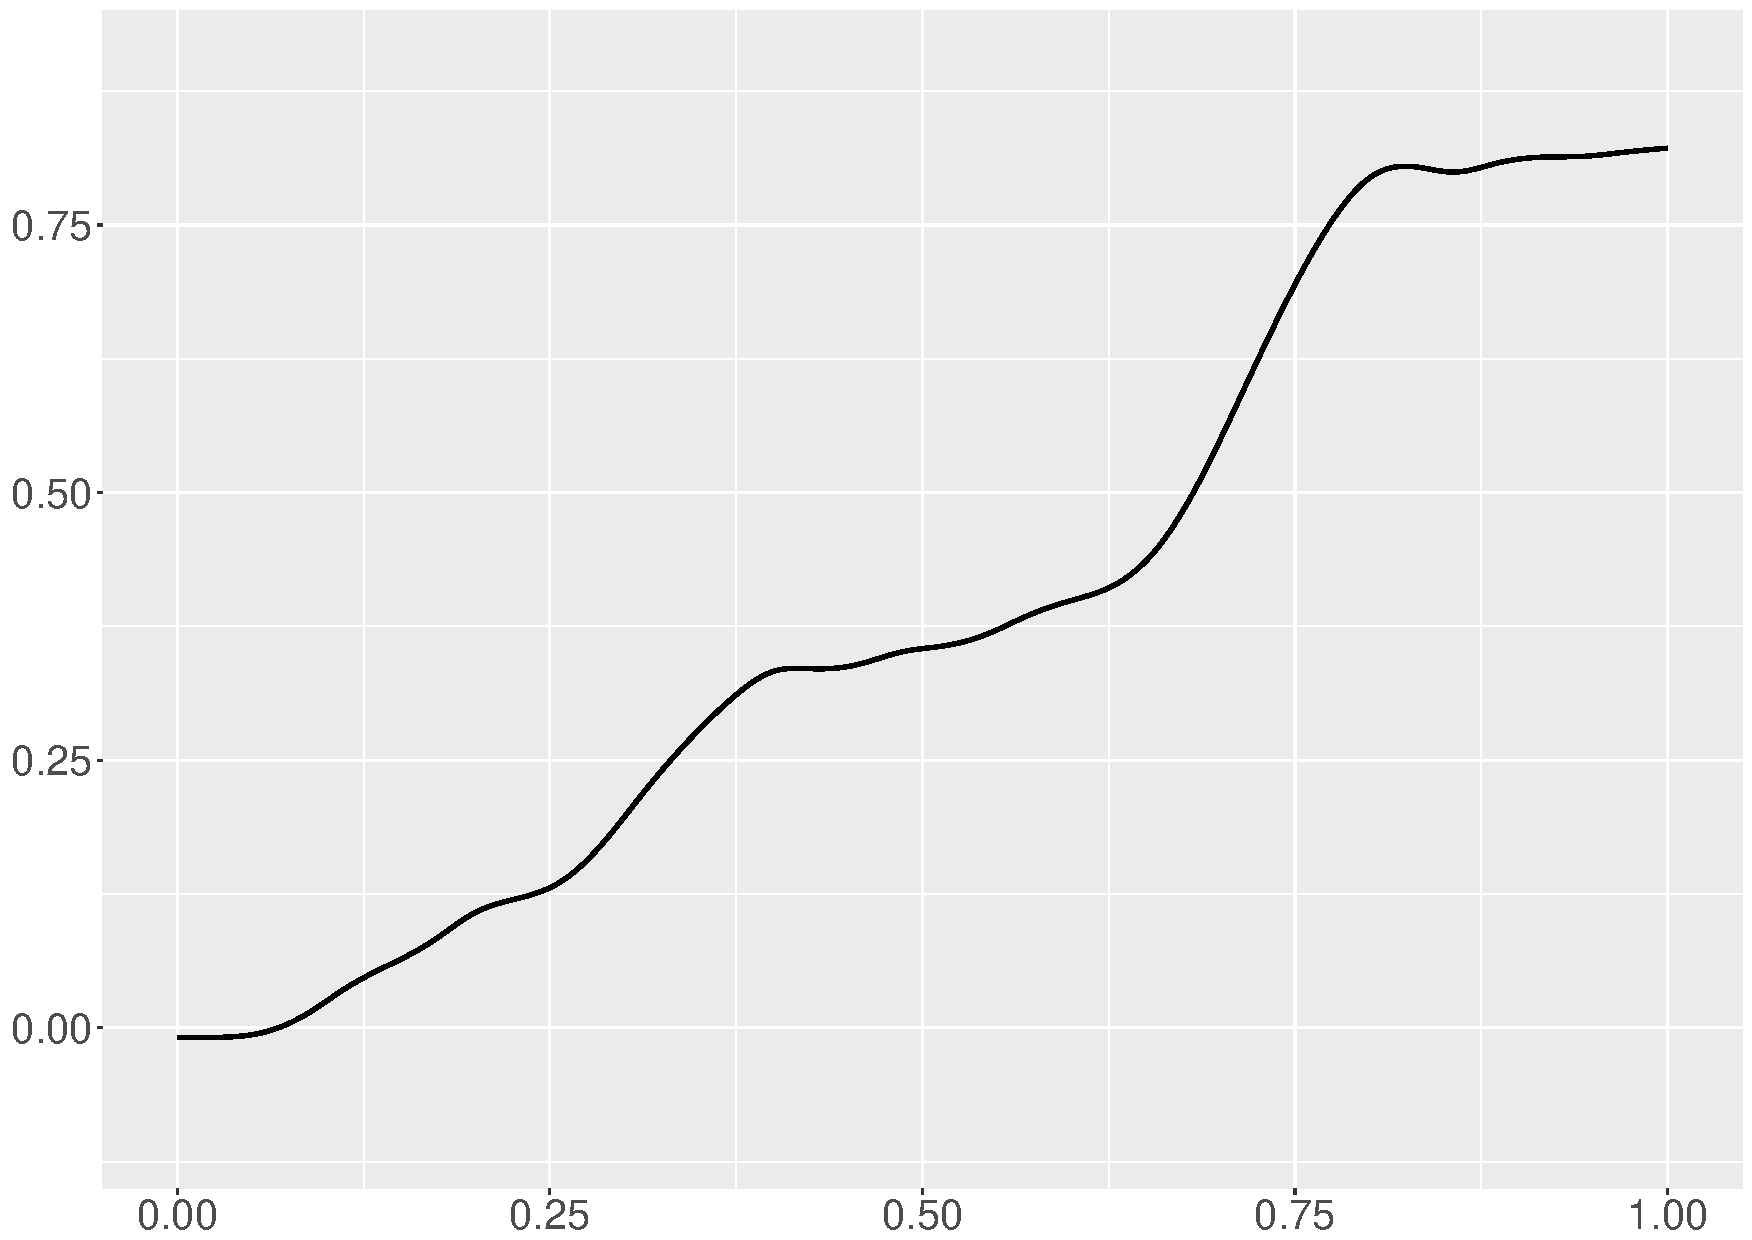
\includegraphics[width=\linewidth,height=0.45\textwidth]{Chapters/02TractorSplineTheory/plot/ggplot/ggBlocksPSpline.pdf}
    \caption{Reconstruction by P-spline \\\mbox{  } }
    \end{subfigure}
    \begin{subfigure}{0.45\textwidth}
    \centering
    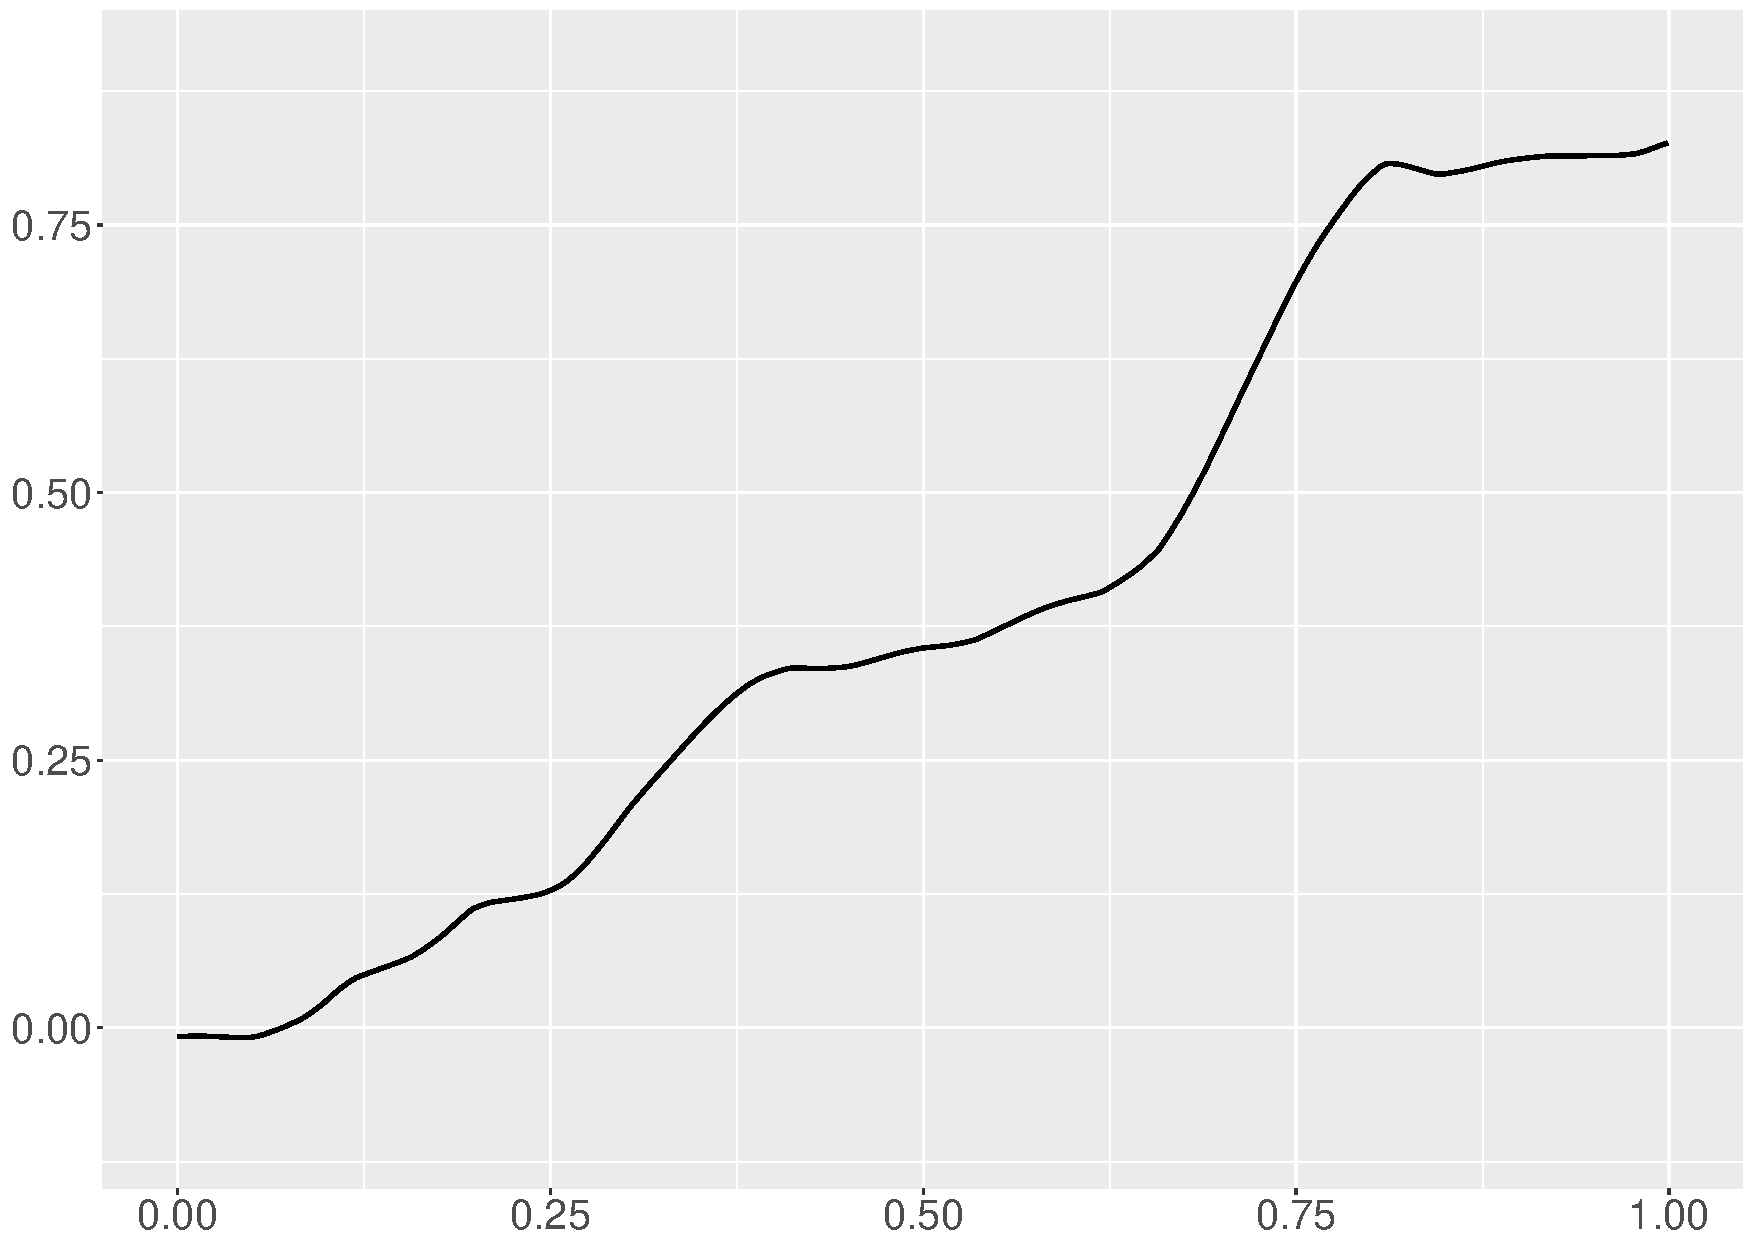
\includegraphics[width=\linewidth,height=0.45\textwidth]{Chapters/02TractorSplineTheory/plot/ggplot/ggBlocksGamma.pdf}
    \caption{Reconstruction by V-spline setting $\gamma=0$}
    \end{subfigure}
  \begin{subfigure}{0.45\textwidth}
    \centering
    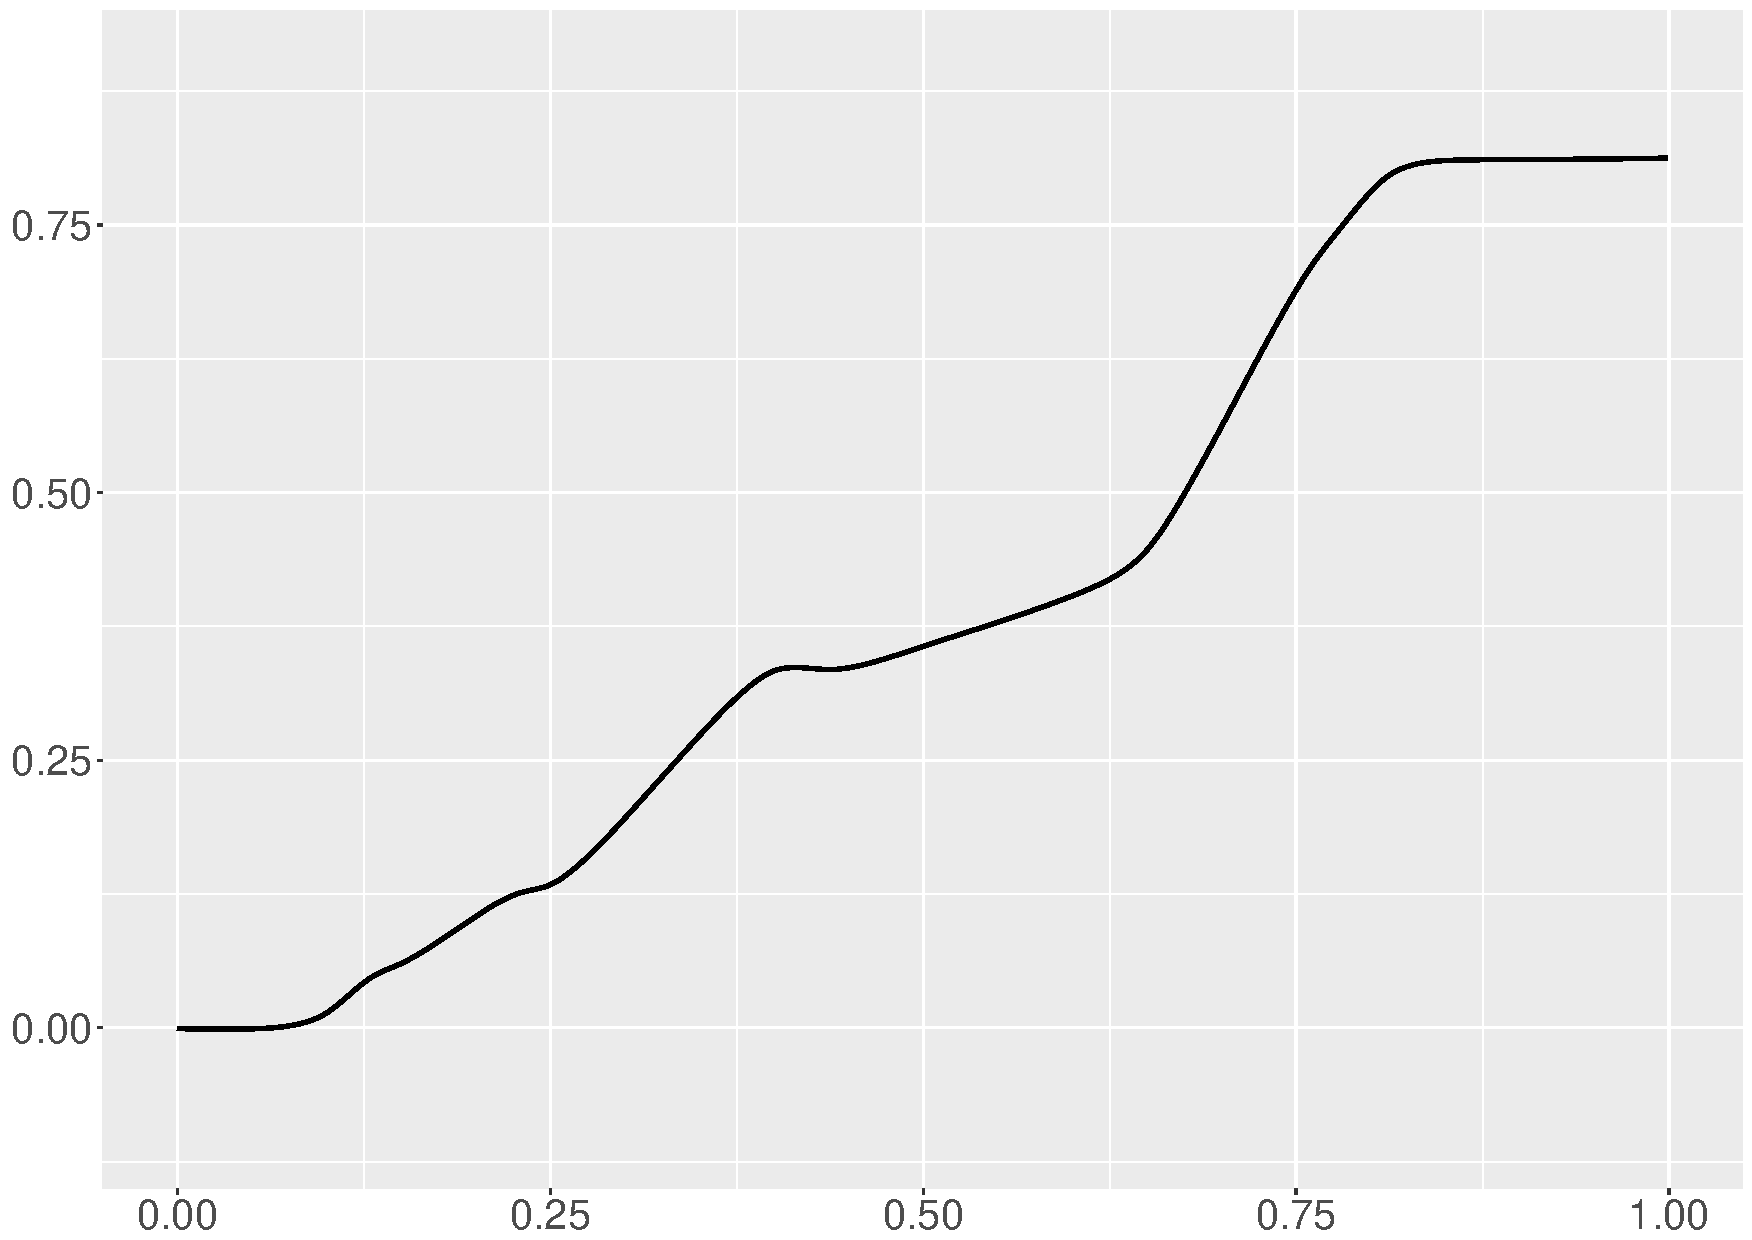
\includegraphics[width=\linewidth,height=0.45\textwidth]{Chapters/02TractorSplineTheory/plot/ggplot/ggBlocksTractorAPT.pdf}
    \caption{Reconstruction by V-spline with conventional penalty term}
    \end{subfigure}
    \begin{subfigure}{0.45\textwidth}
    \centering
    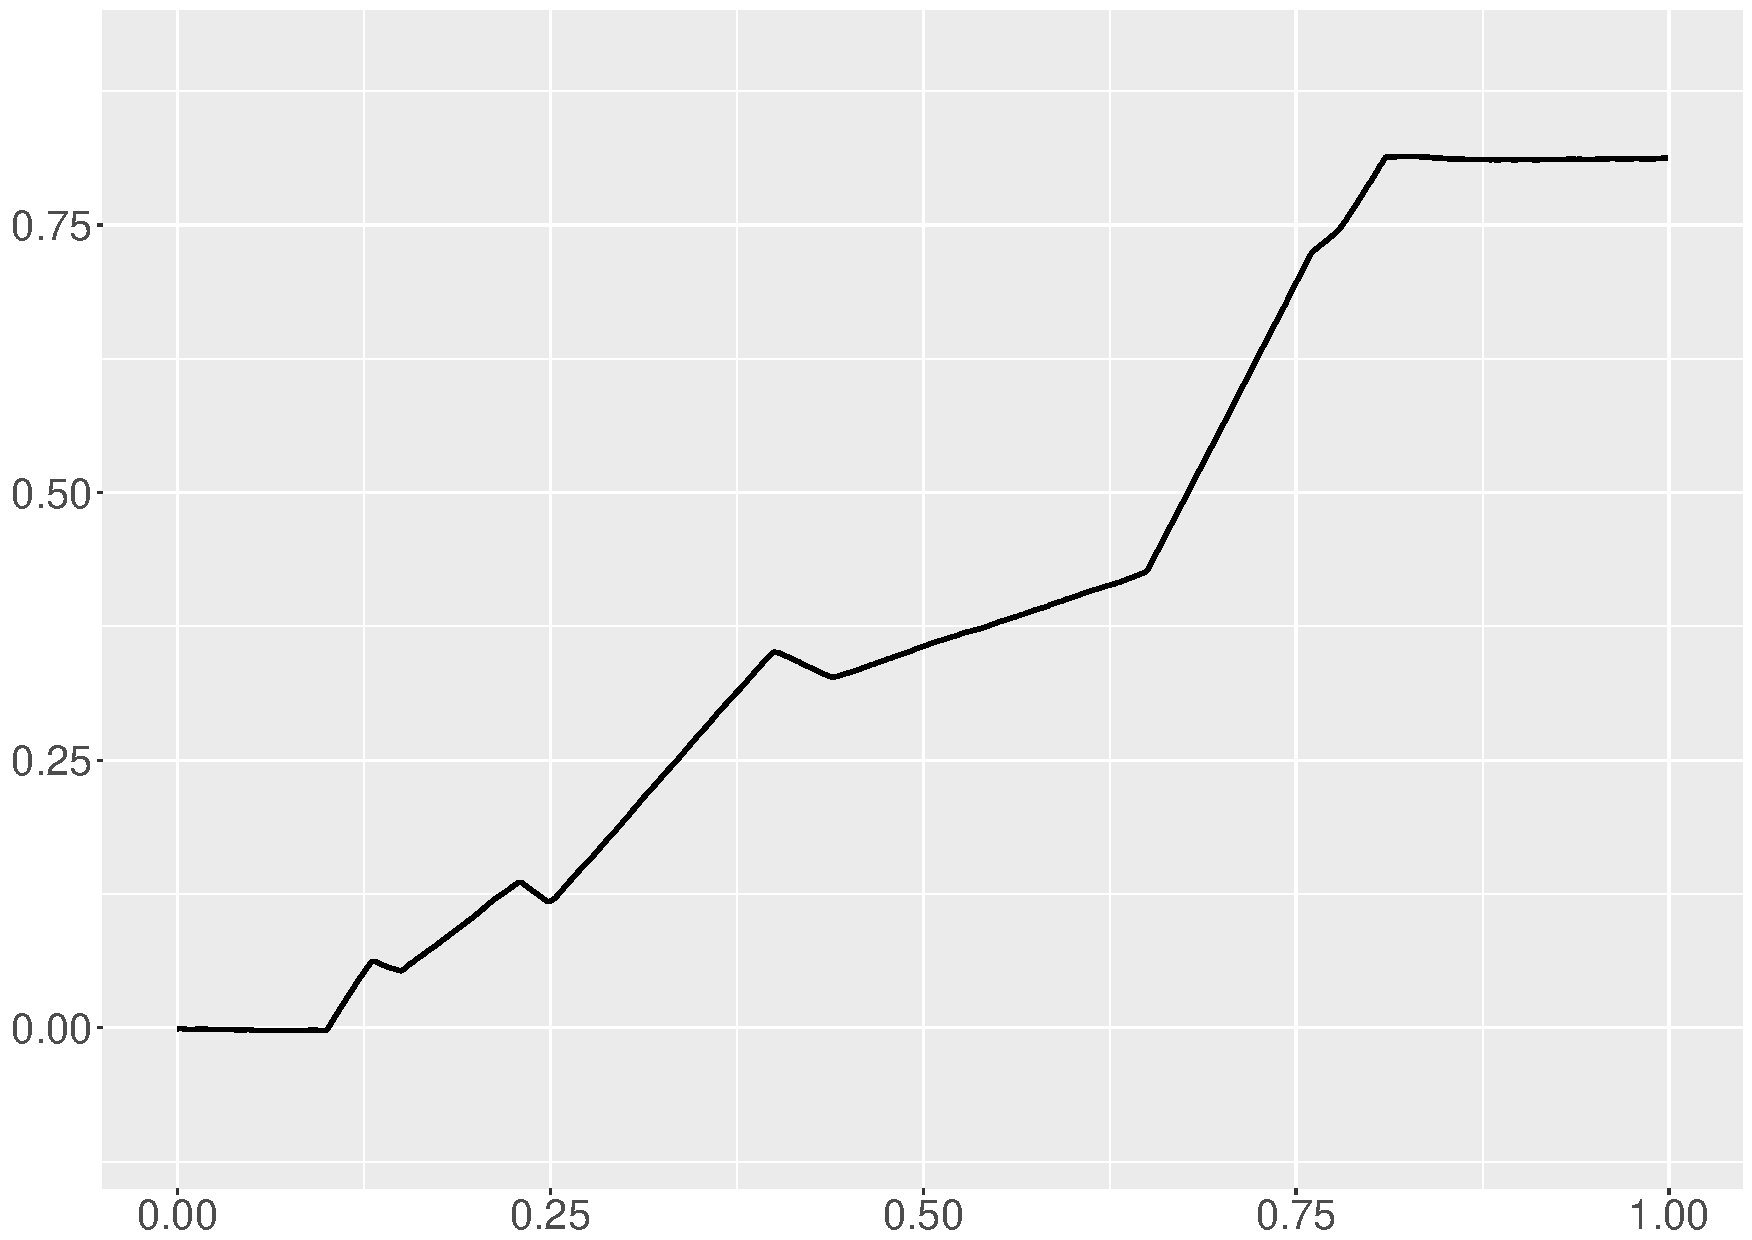
\includegraphics[width=\linewidth,height=0.45\textwidth]{Chapters/02TractorSplineTheory/plot/ggplot/ggBlocksTractor.pdf}
    \caption{Reconstruction by the proposed V-spline}
    \end{subfigure}
\caption{Numerical example: $\textit{Blocks}$. Comparison of different reconstruction methods with simulated data.}\label{num1}
 \end{figure}

%
%\begin{figure}
%  \centering
%    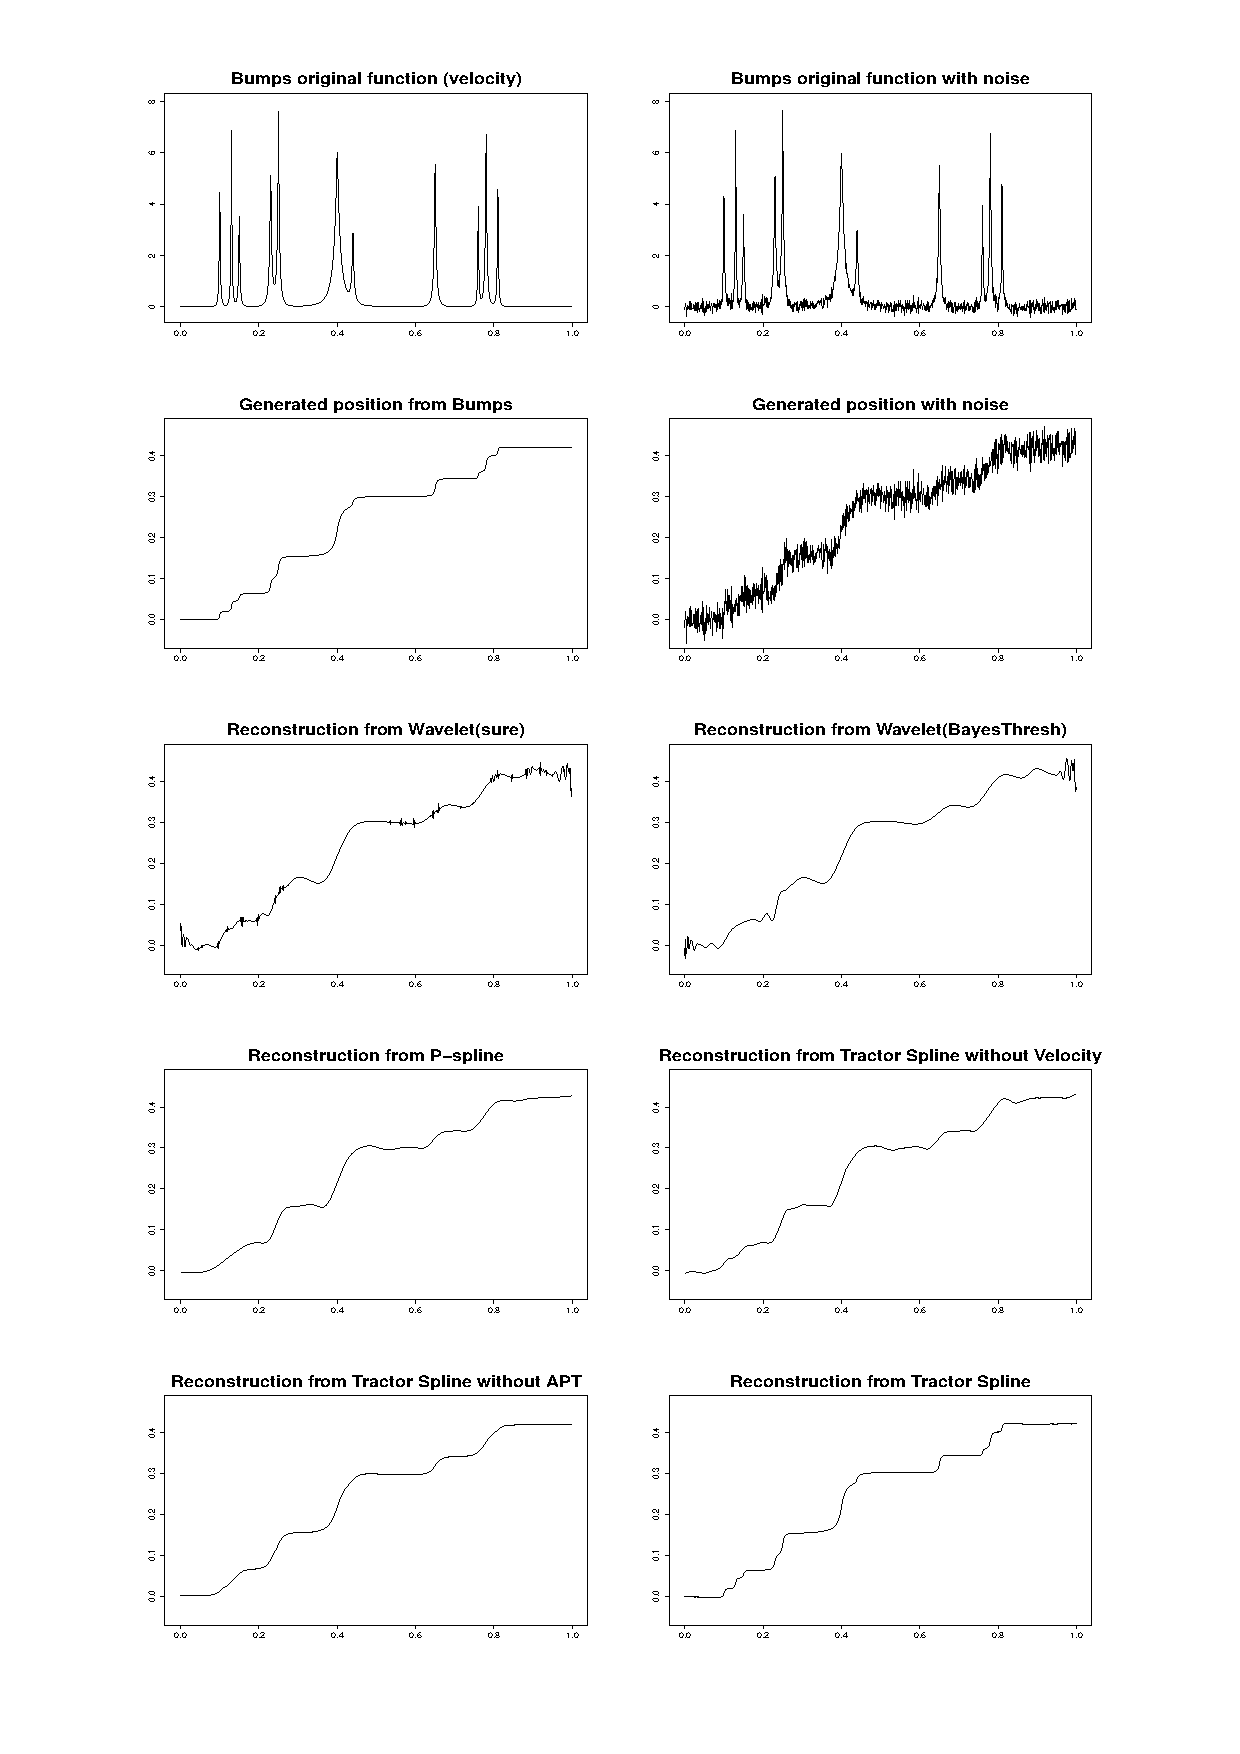
\includegraphics[width=\textwidth,height=14cm]{Chapters/02TractorSplineTheory/plot/bumps10}
%  \caption{Numerical example: $\textit{Bumps}$. (a) The true velocity function. (b) Velocity with Gaussian noise at SNR=7. (c) Generated position function. (d) Position with Gaussian noise at SNR=7. (e) Reconstruction from Wavelet with sure threshold. (f) Reconstruction from Wavelet with BayesThresh approach. (g) Reconstruction by P-spline. (h) Reconstruction by V-spline setting $\gamma=0$. (i) Reconstruction by V-spline with normal penalty term. (j) Reconstruction by proposed V-spline.}\label{num2}
%\end{figure}


\begin{figure}
    \centering
    \begin{subfigure}{0.45\textwidth}
    \centering
    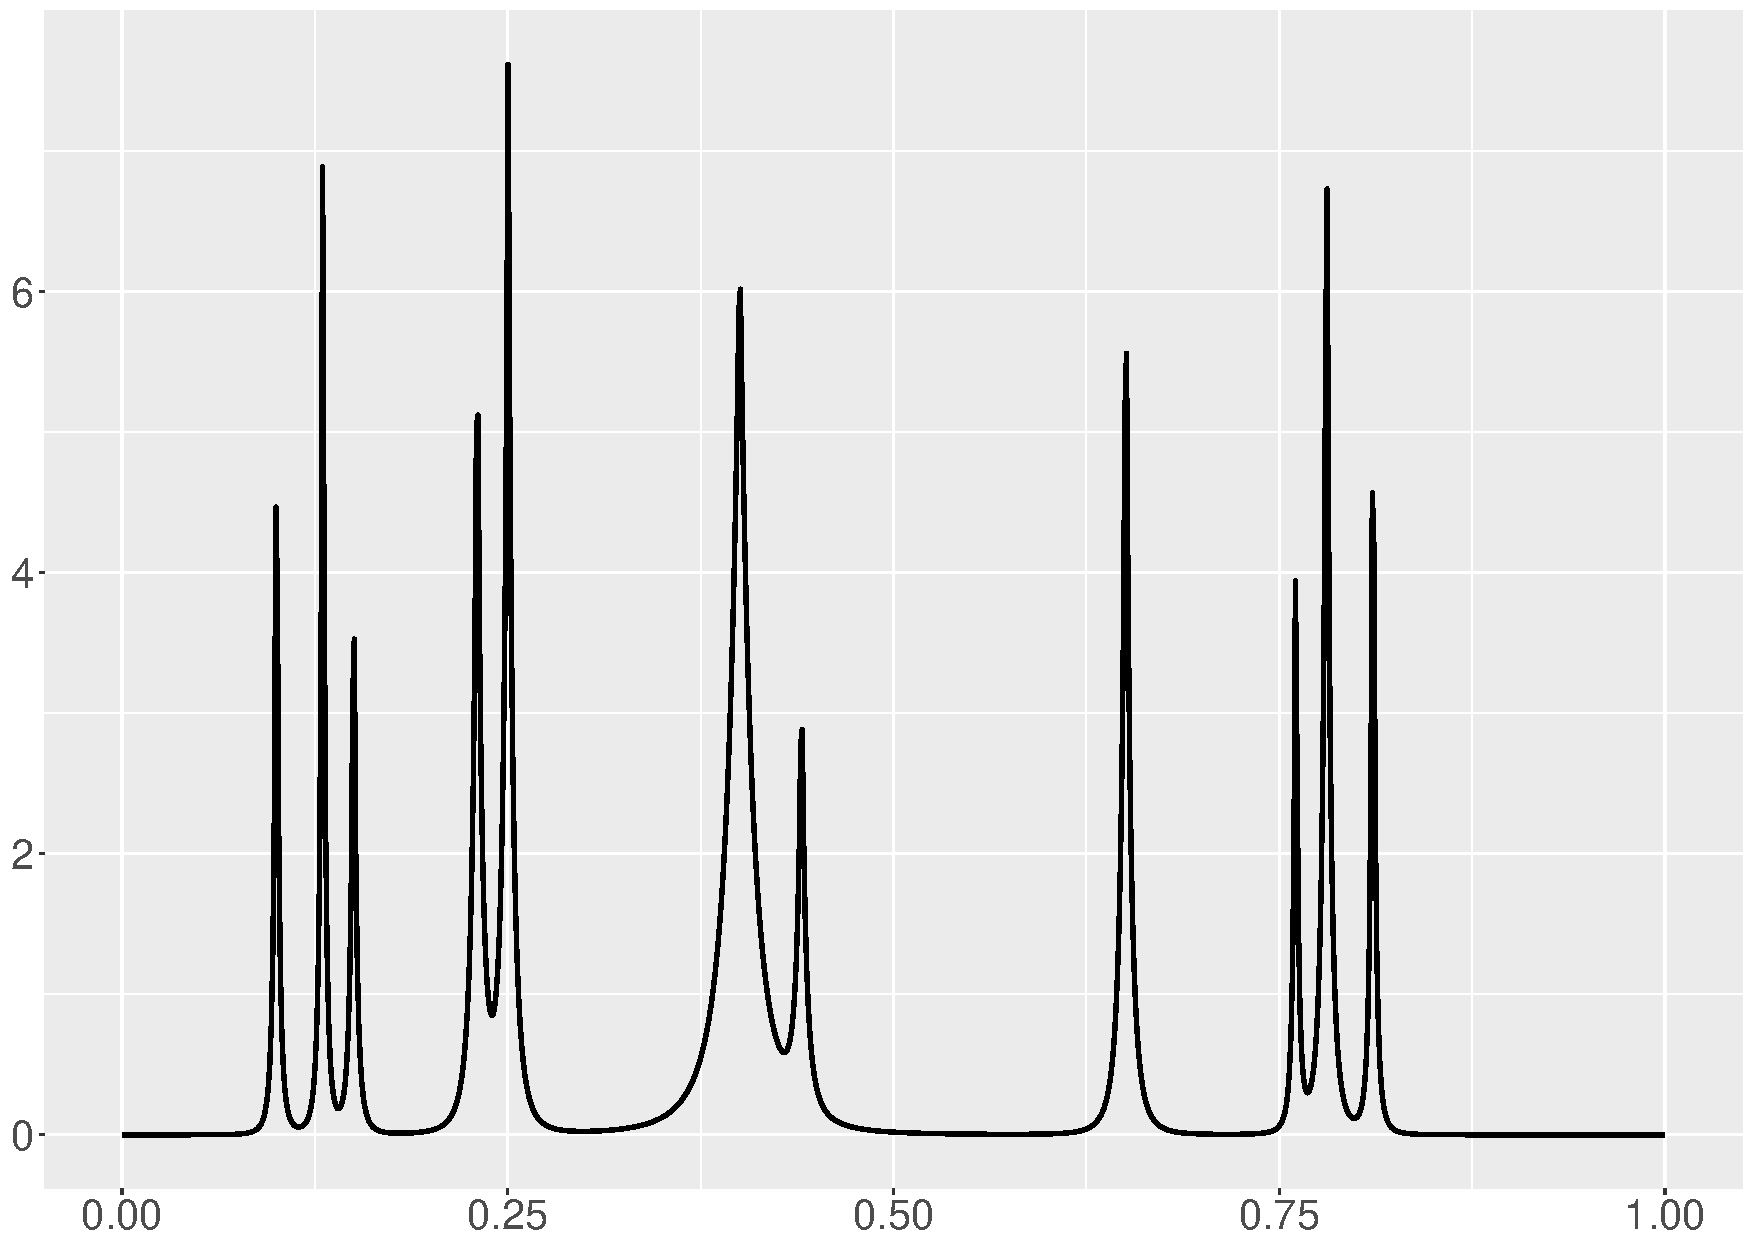
\includegraphics[width=\linewidth,height=0.45\textwidth]{Chapters/02TractorSplineTheory/plot/ggplot/ggBumps.pdf}
    \caption{True \textit{Bumps} function}
    \end{subfigure}%
    \begin{subfigure}{0.45\textwidth}
    \centering
    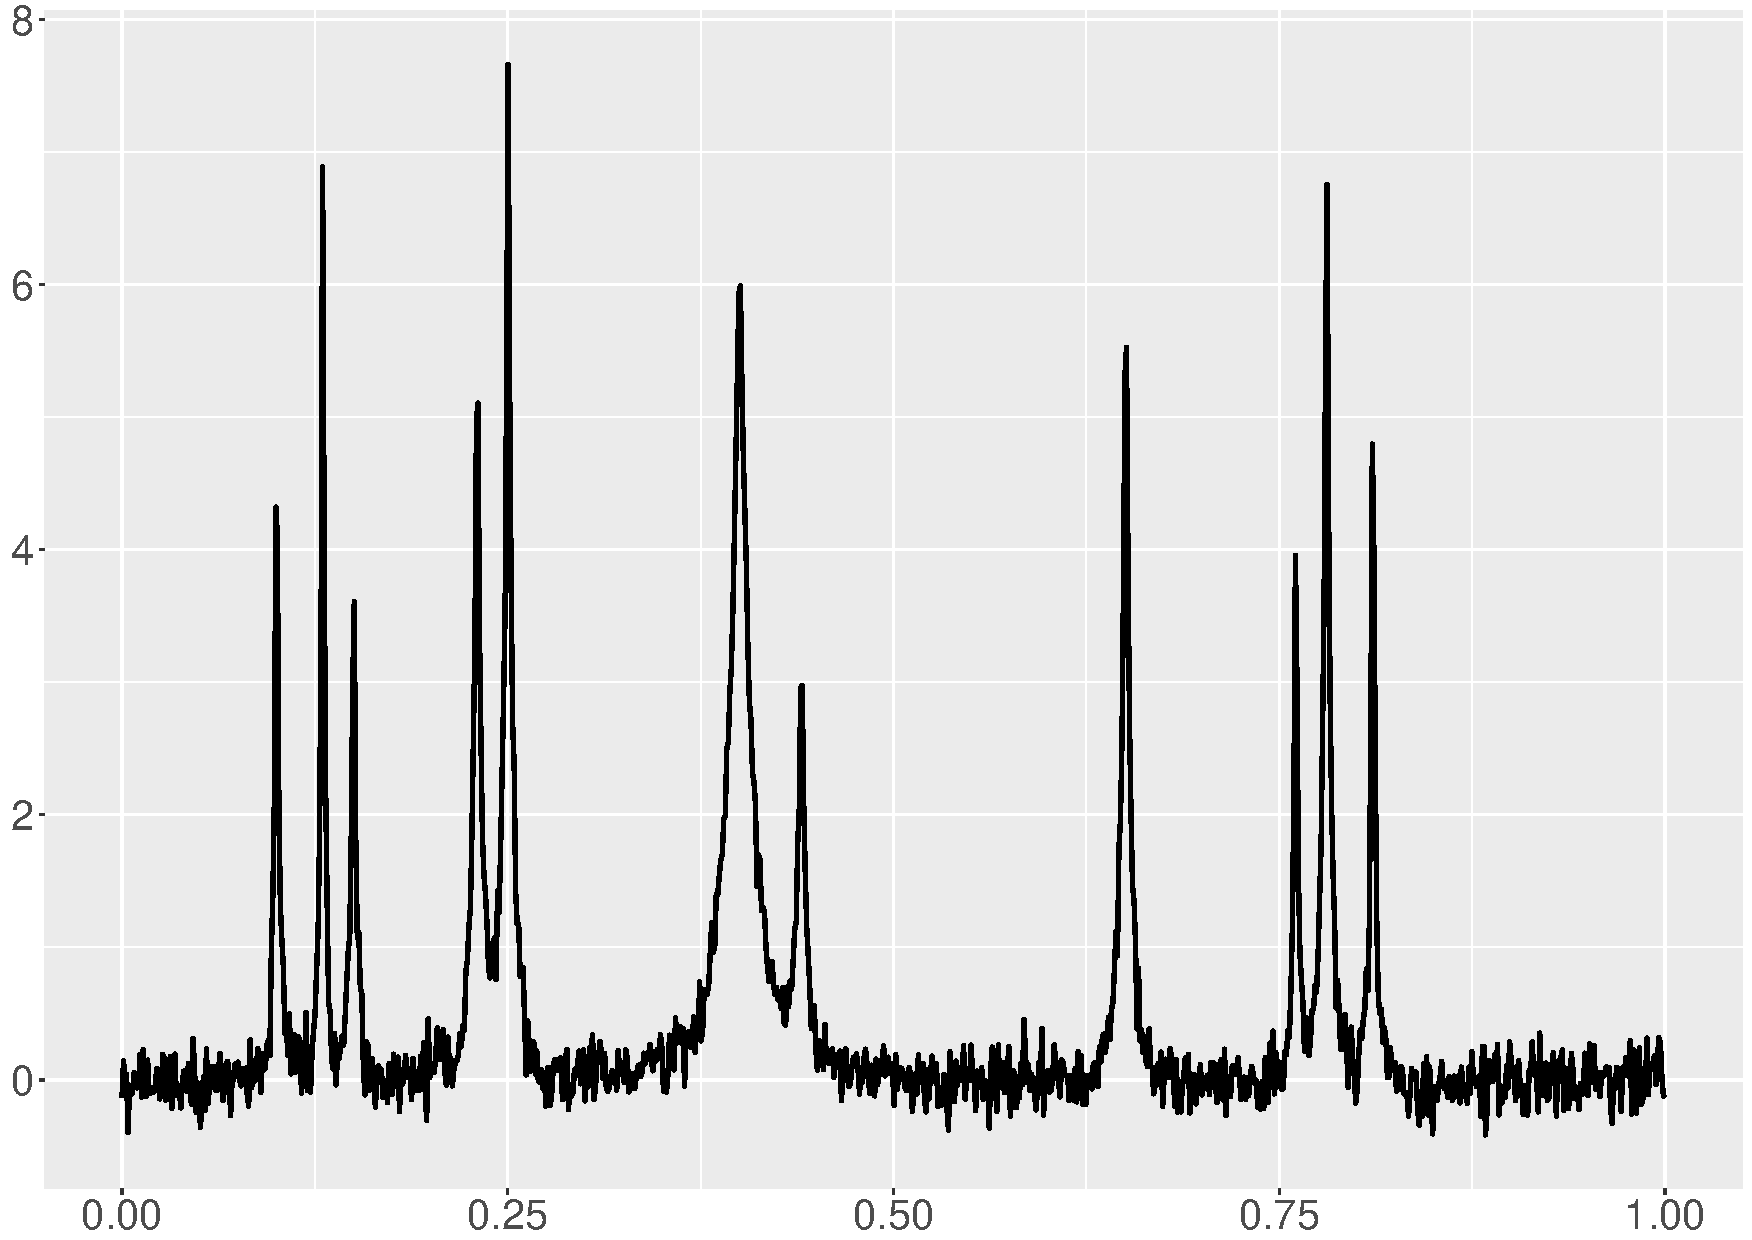
\includegraphics[width=\linewidth,,height=0.45\textwidth]{Chapters/02TractorSplineTheory/plot/ggplot/ggBumpsNoise.pdf}
    \caption{Noisy \textit{Bumps} at \textit{SNR}=7}
    \end{subfigure}
    \begin{subfigure}{0.45\textwidth}
    \centering
    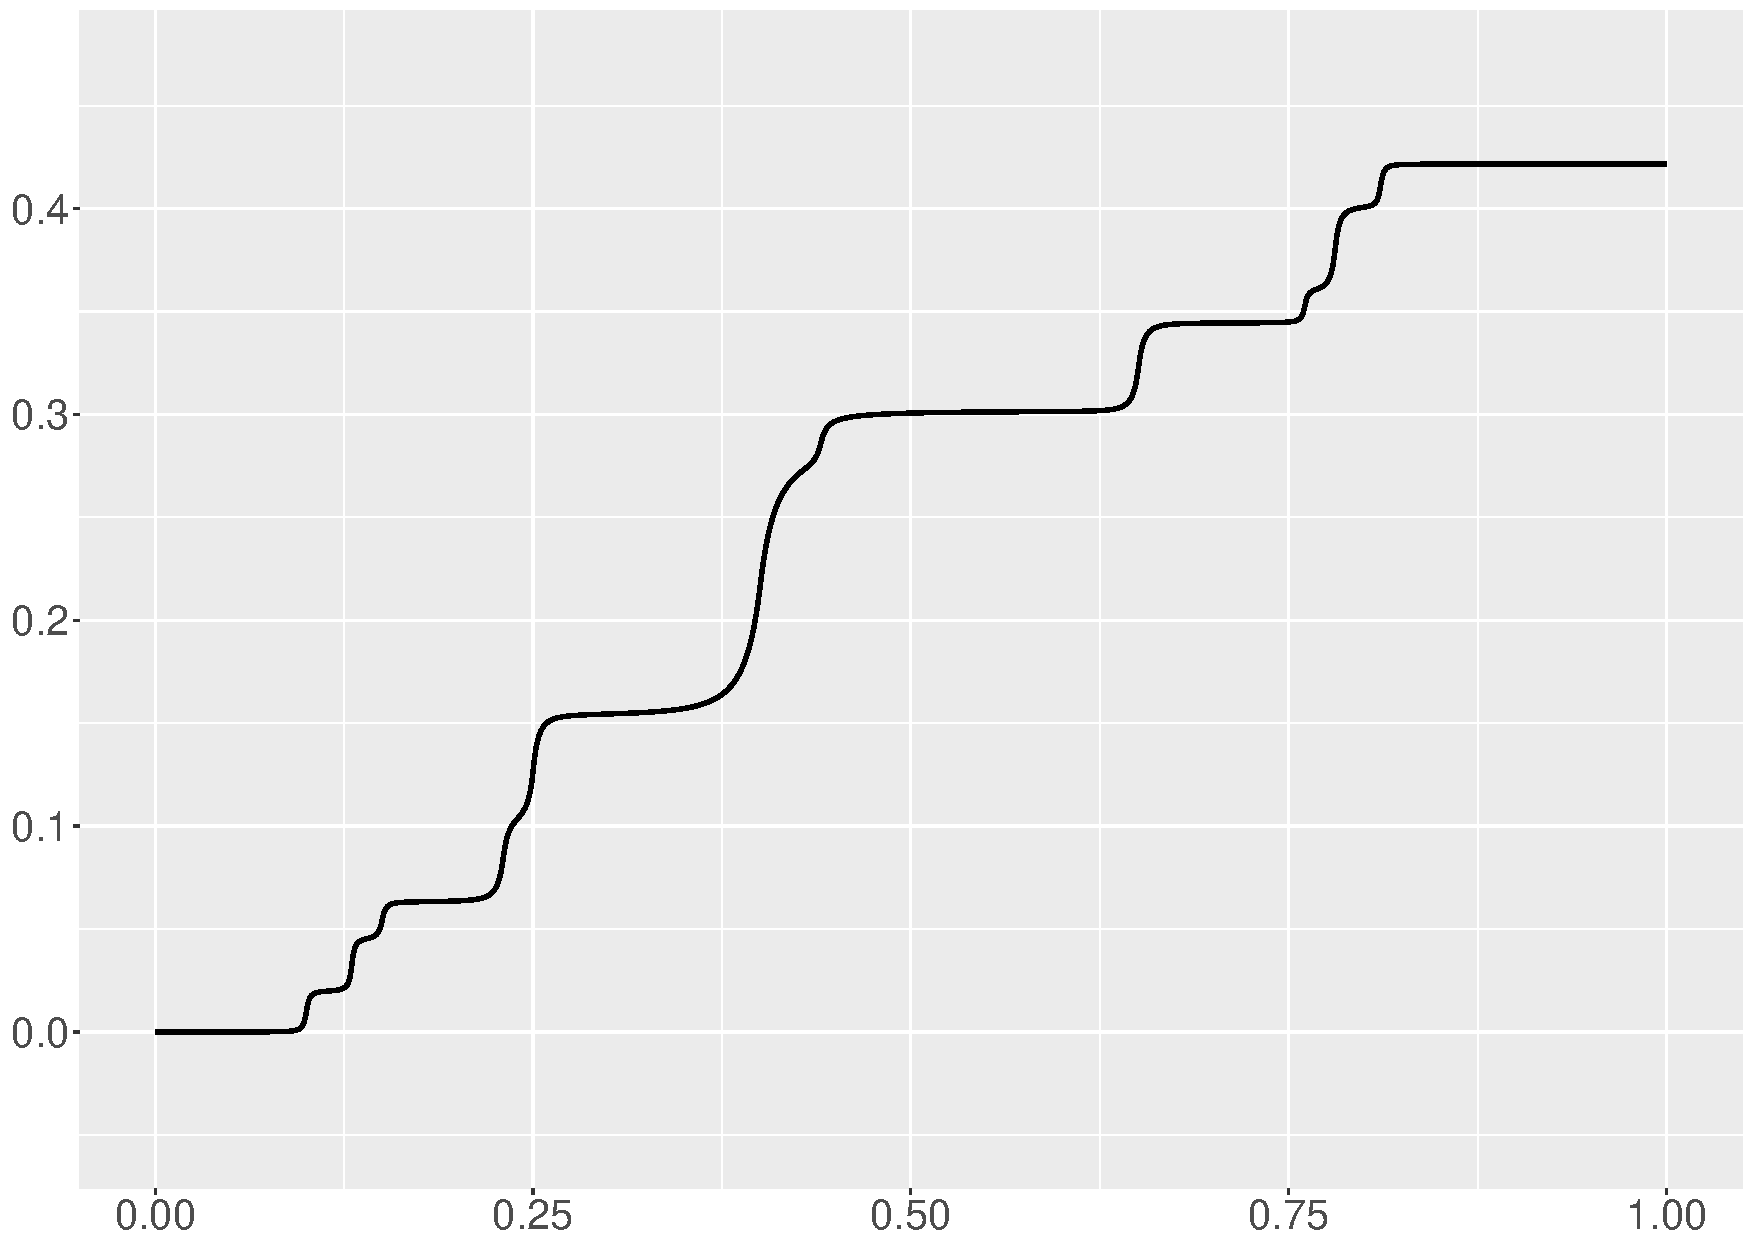
\includegraphics[width=\linewidth,height=0.45\textwidth]{Chapters/02TractorSplineTheory/plot/ggplot/ggBumpsPosition.pdf}
    \caption{Generated positions}
    \end{subfigure}
    \begin{subfigure}{0.45\textwidth}
    \centering
    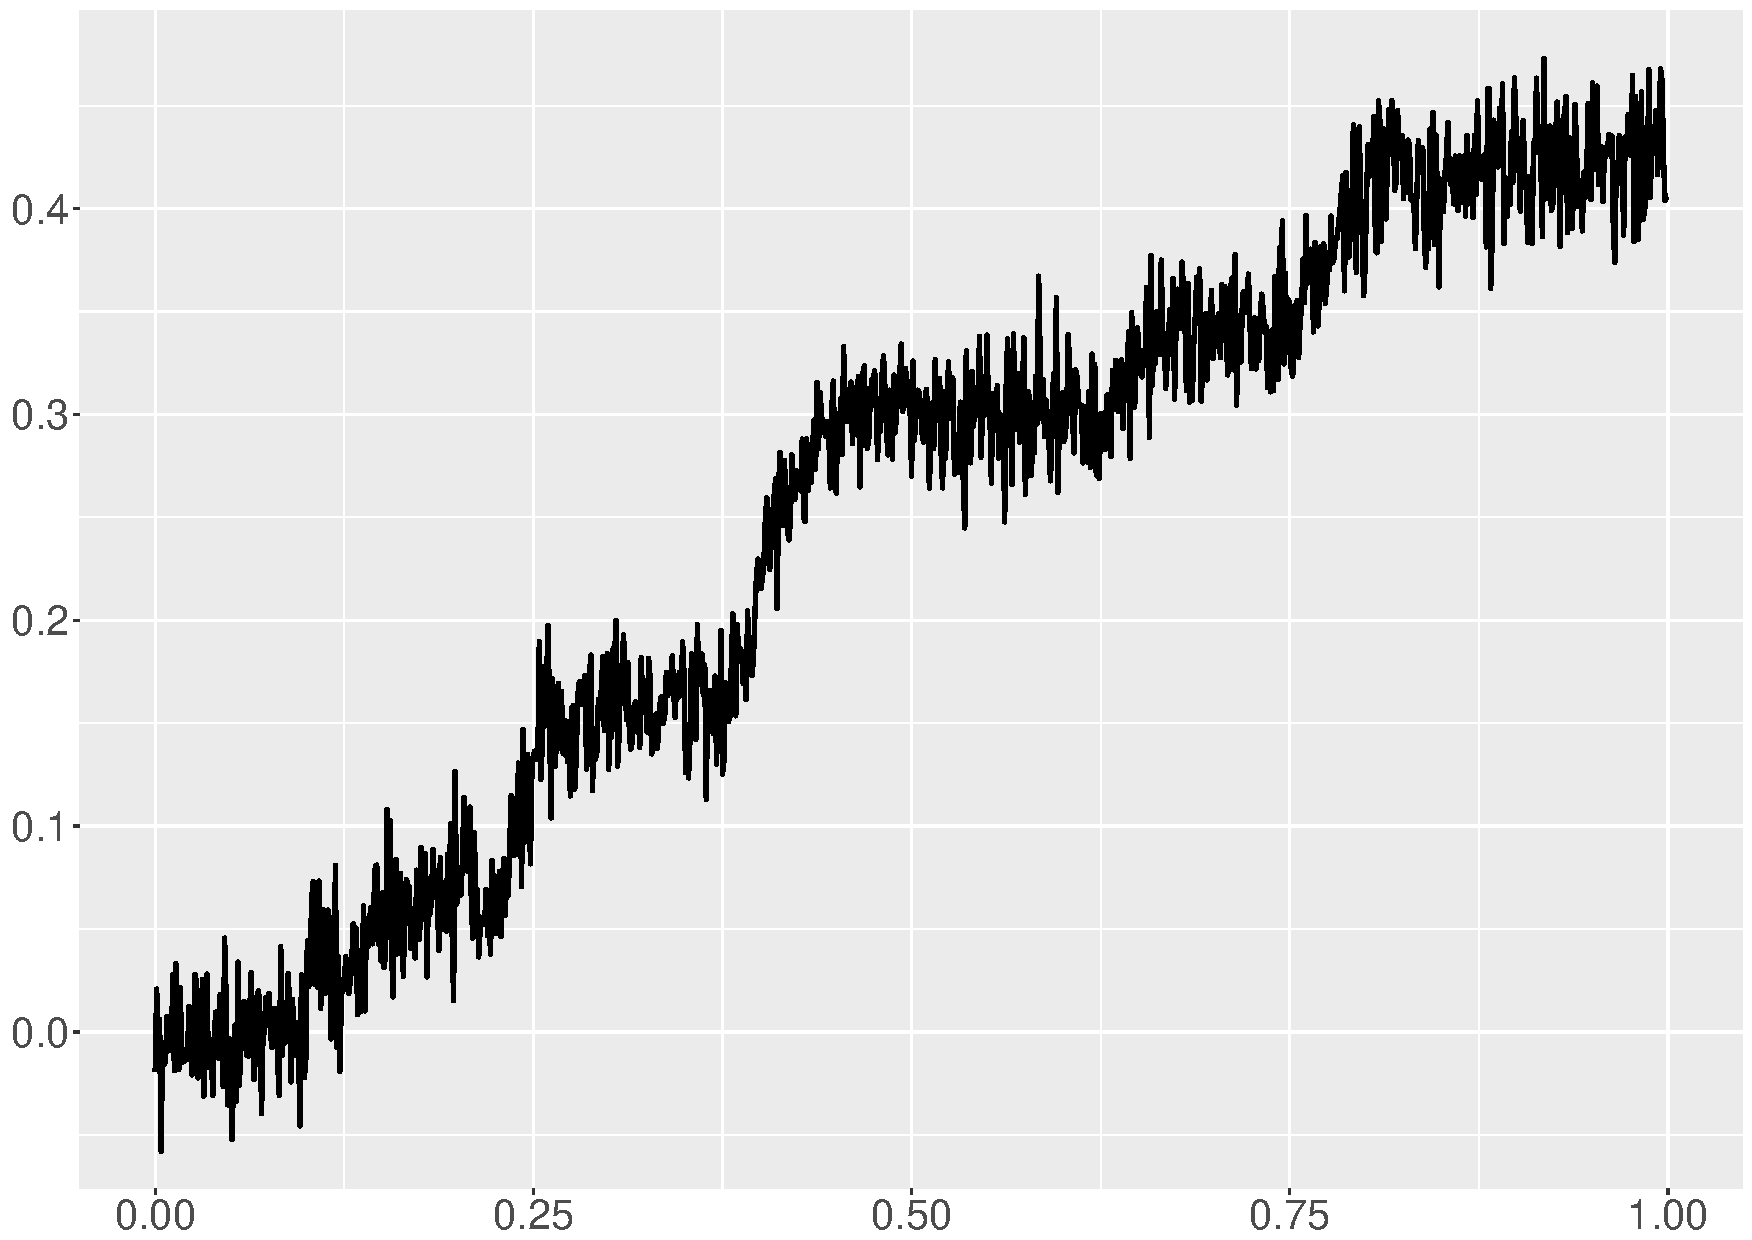
\includegraphics[width=\linewidth,height=0.45\textwidth]{Chapters/02TractorSplineTheory/plot/ggplot/ggBumpsPositionNoise.pdf}
    \caption{Noisy position at \textit{SNR}=7}
    \end{subfigure}
    \begin{subfigure}{0.45\textwidth}
    \centering
    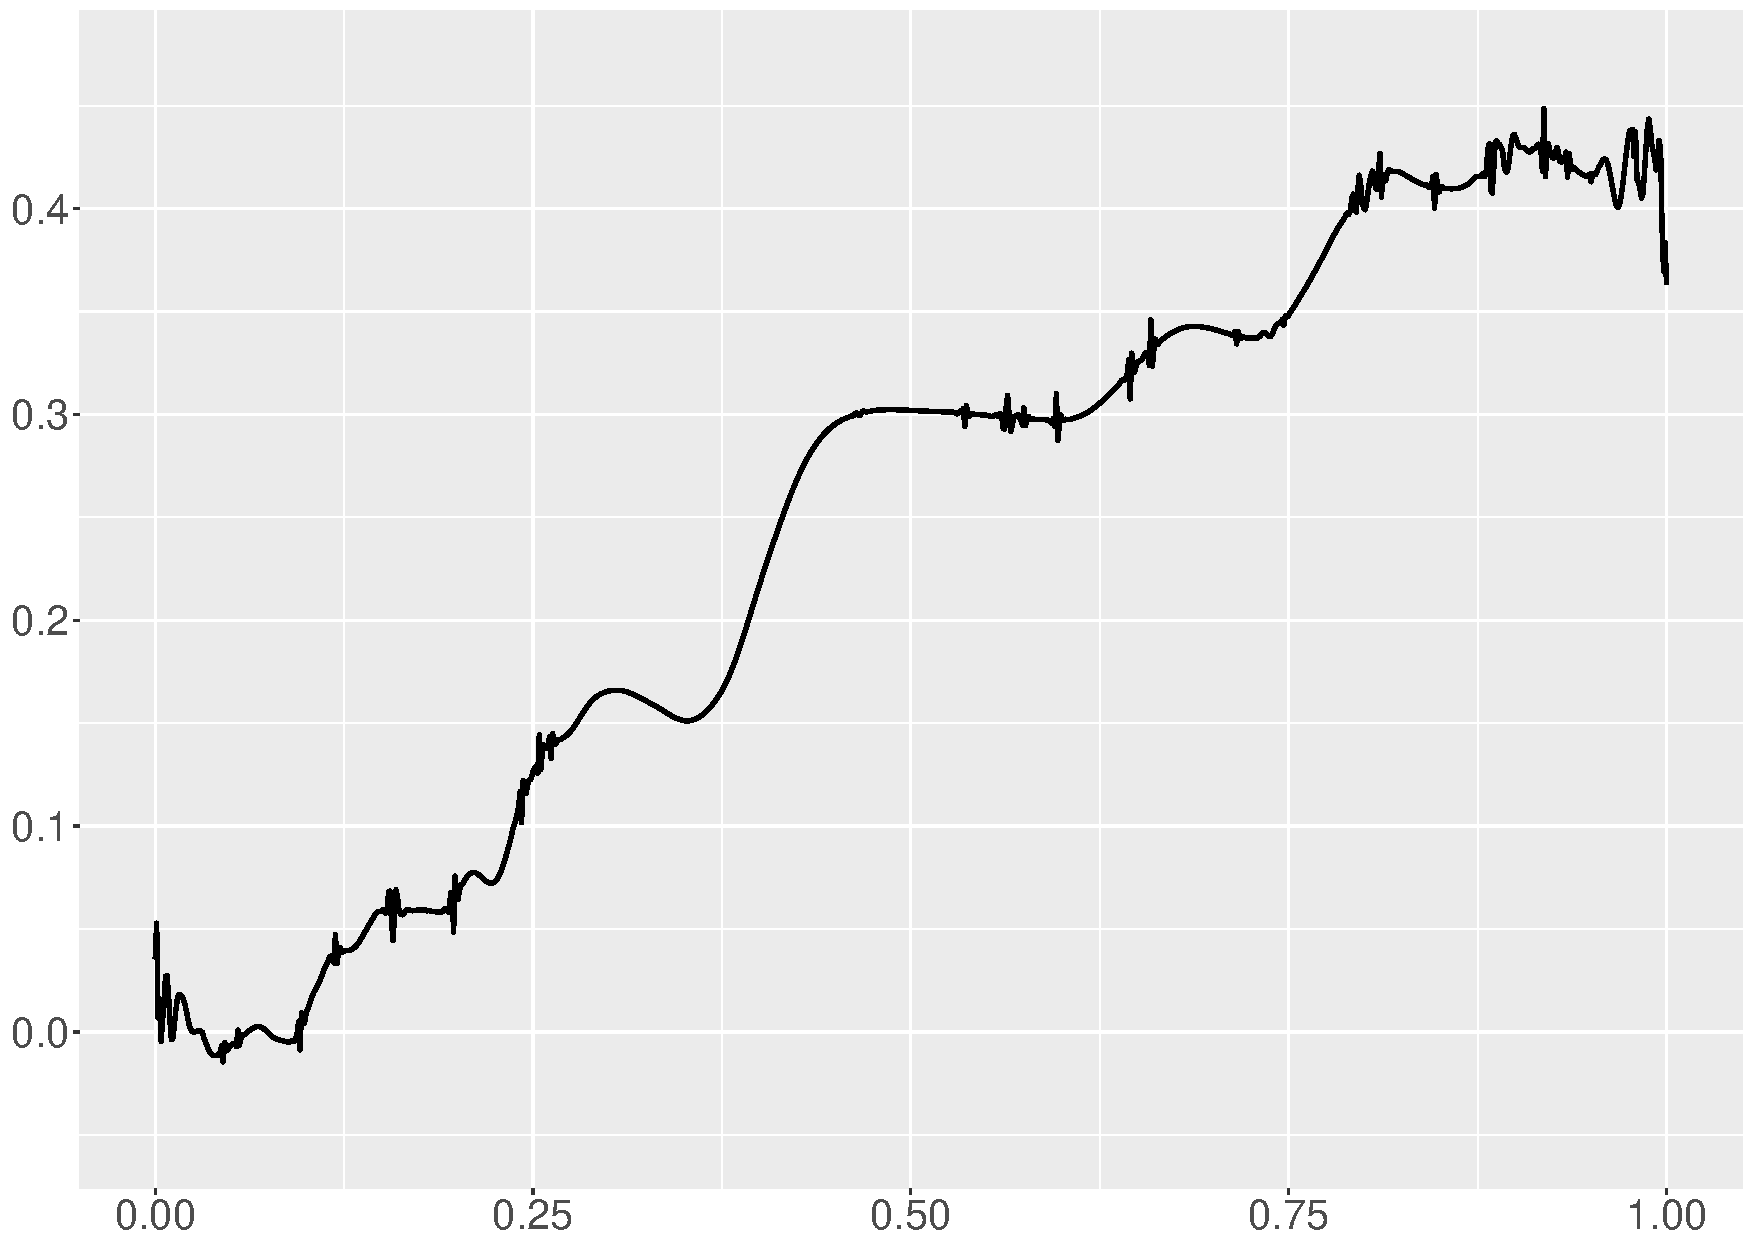
\includegraphics[width=\linewidth,height=0.45\textwidth]{Chapters/02TractorSplineTheory/plot/ggplot/ggBumpsSure.pdf}
    \caption{Reconstruction from Wavelet by sure threshold}
    \end{subfigure}
    \begin{subfigure}{0.45\textwidth}
    \centering
    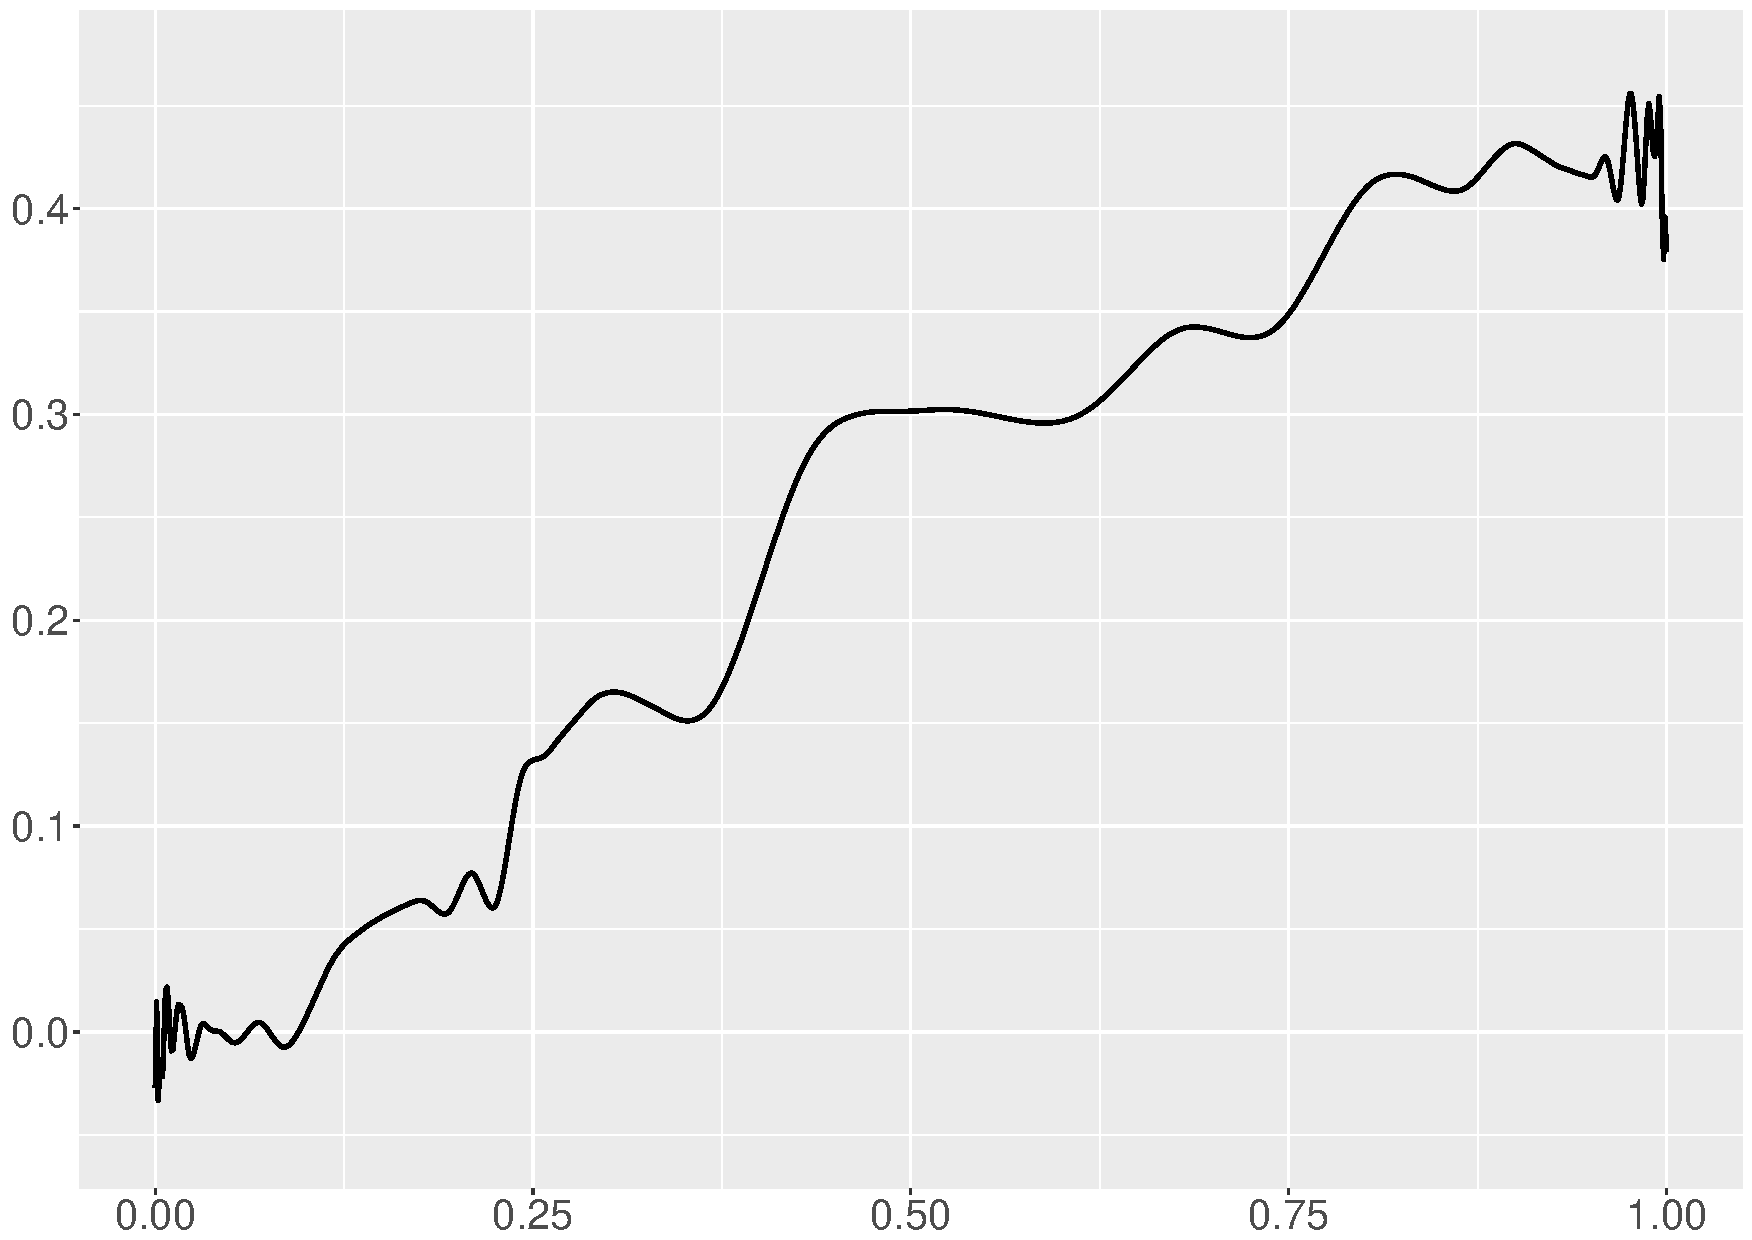
\includegraphics[width=\linewidth,height=0.45\textwidth]{Chapters/02TractorSplineTheory/plot/ggplot/ggBumpsBayes.pdf}
    \caption{Reconstruction from Wavelet by BayesThresh approach}
    \end{subfigure}
    \begin{subfigure}{0.45\textwidth}
    \centering
    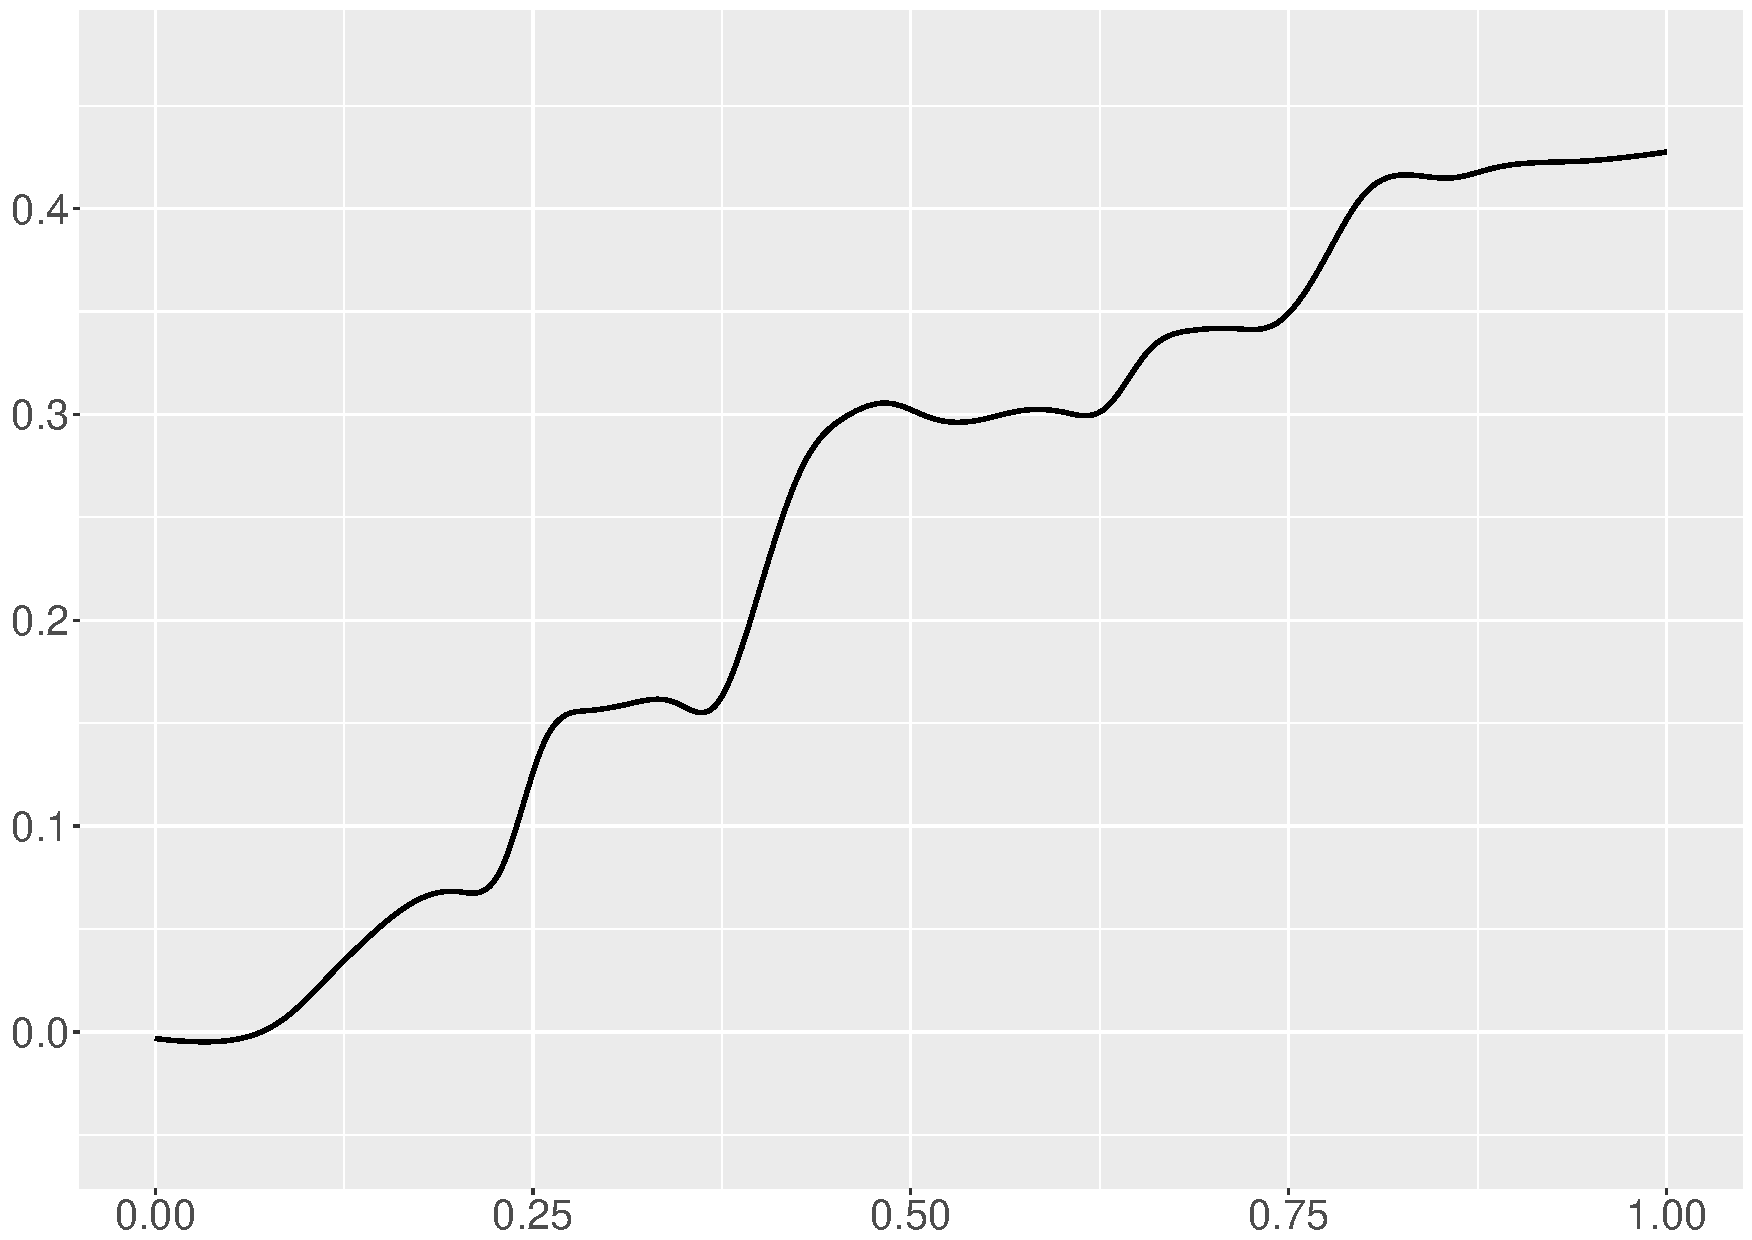
\includegraphics[width=\linewidth,height=0.45\textwidth]{Chapters/02TractorSplineTheory/plot/ggplot/ggBumpsPSpline.pdf}
    \caption{Reconstruction by P-spline \\\mbox{  } }
    \end{subfigure}
    \begin{subfigure}{0.45\textwidth}
    \centering
    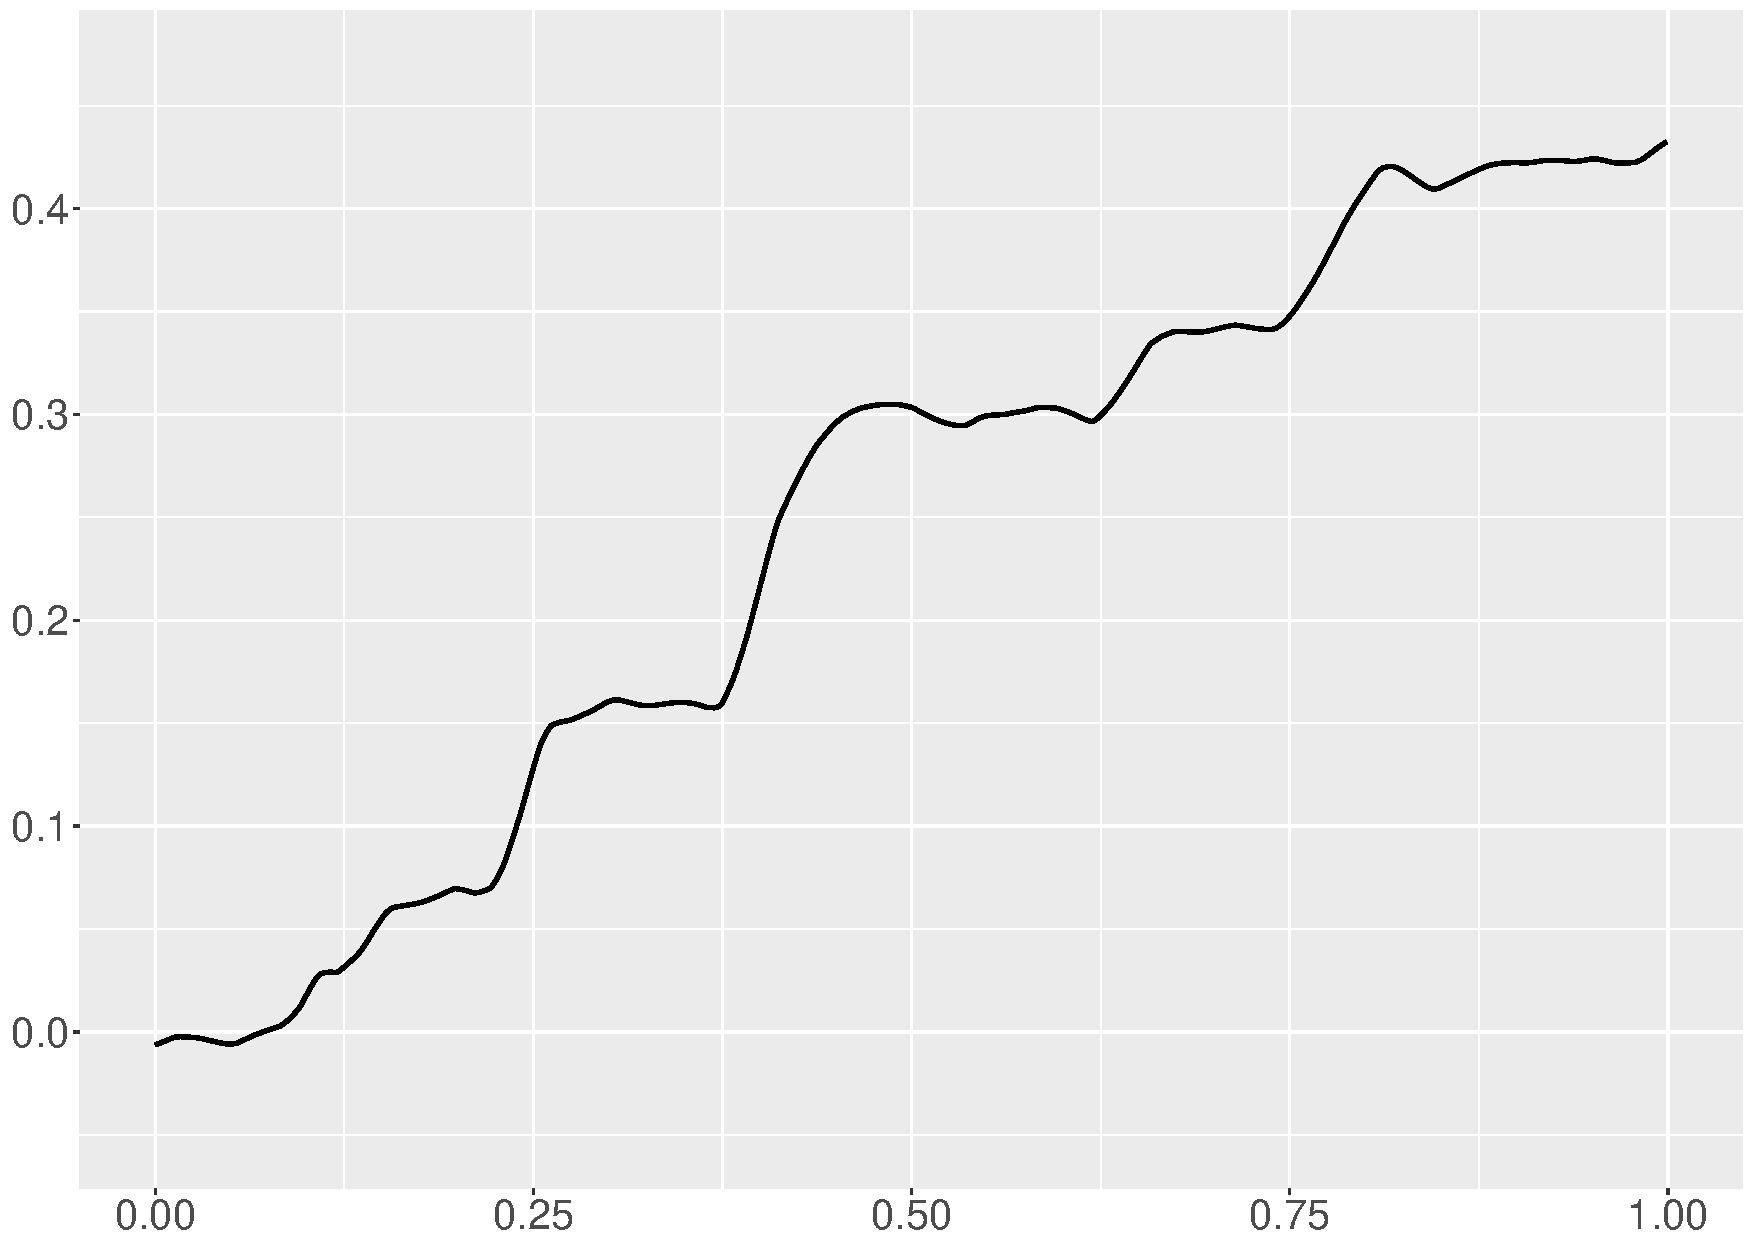
\includegraphics[width=\linewidth,height=0.45\textwidth]{Chapters/02TractorSplineTheory/plot/ggplot/ggBumpsGamma.pdf}
    \caption{Reconstruction by V-spline setting $\gamma=0$}
    \end{subfigure}
  \begin{subfigure}{0.45\textwidth}
    \centering
    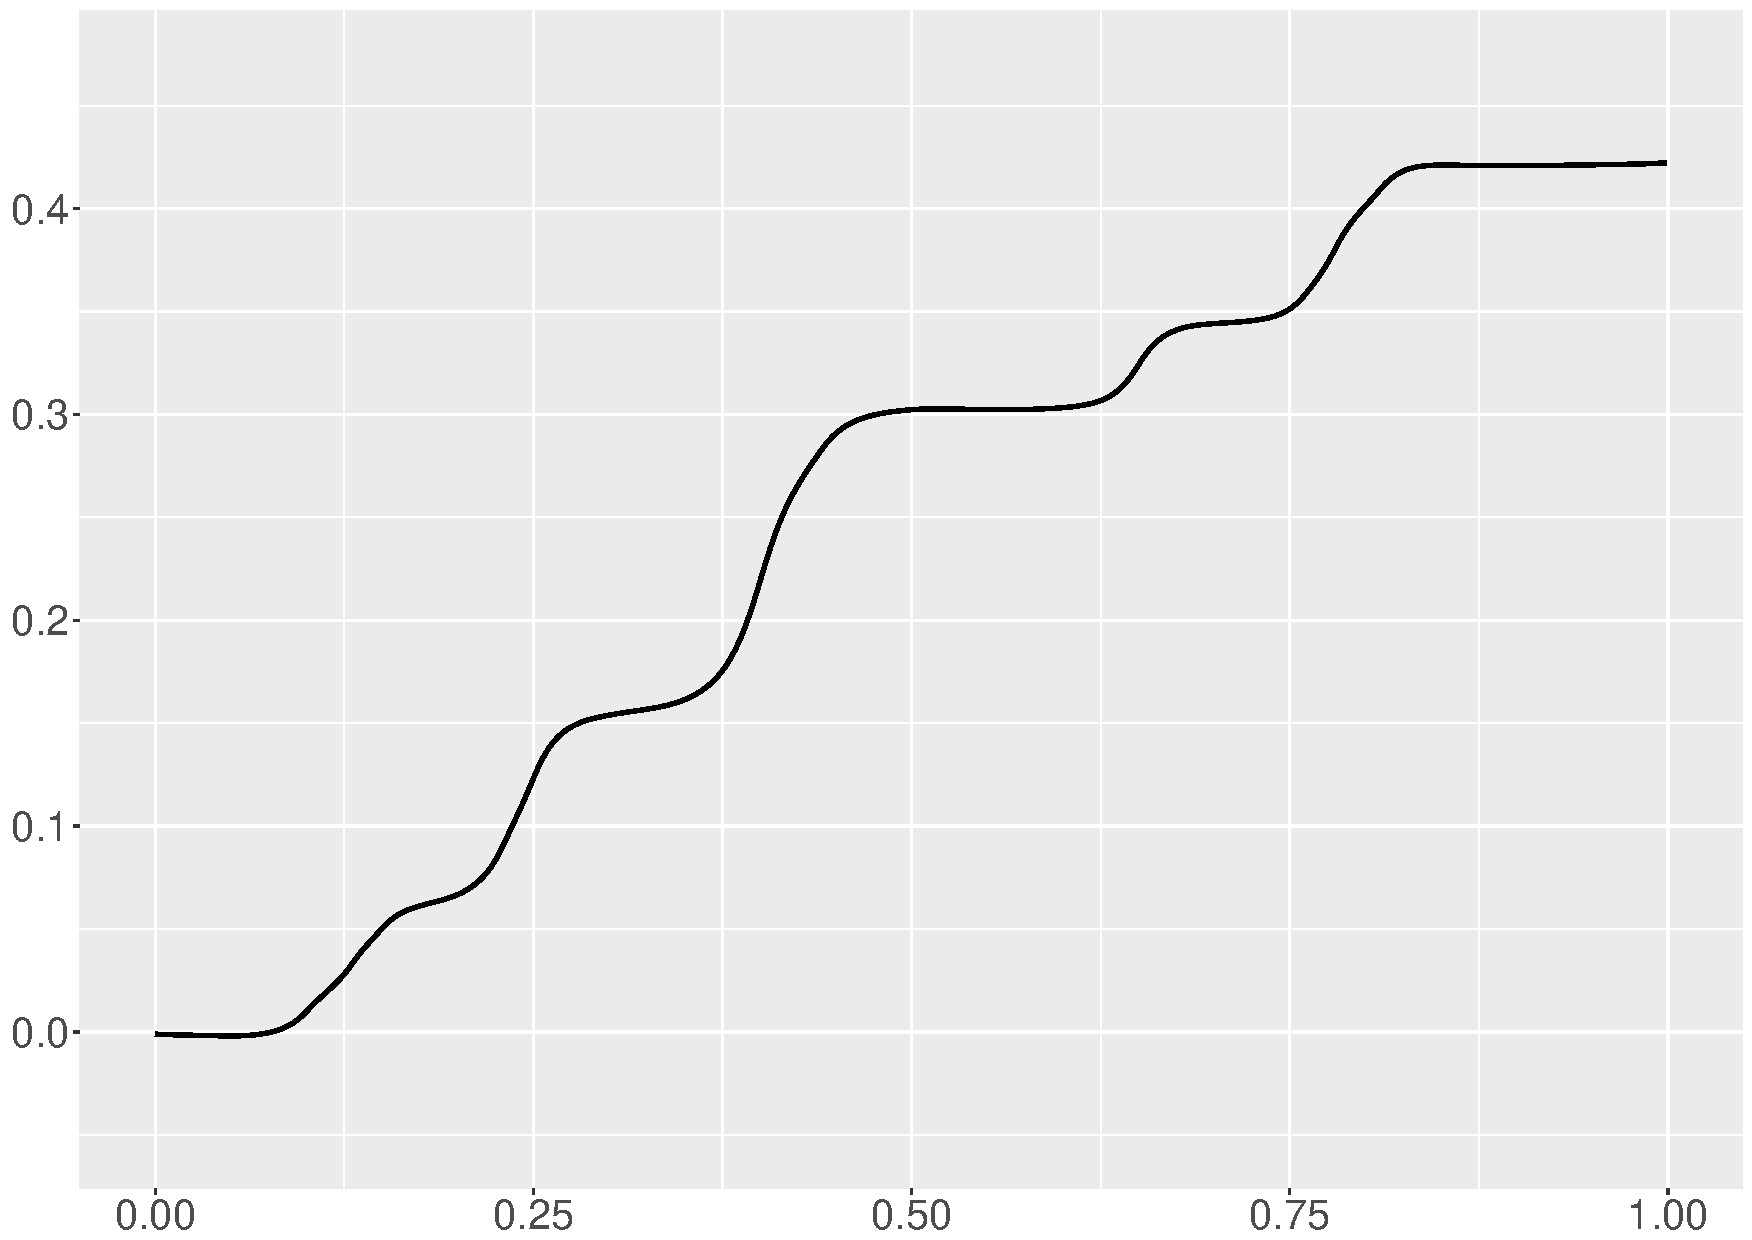
\includegraphics[width=\linewidth,height=0.45\textwidth]{Chapters/02TractorSplineTheory/plot/ggplot/ggBumpsTractorAPT.pdf}
    \caption{Reconstruction by V-spline with conventional penalty term}
    \end{subfigure}
    \begin{subfigure}{0.45\textwidth}
    \centering
    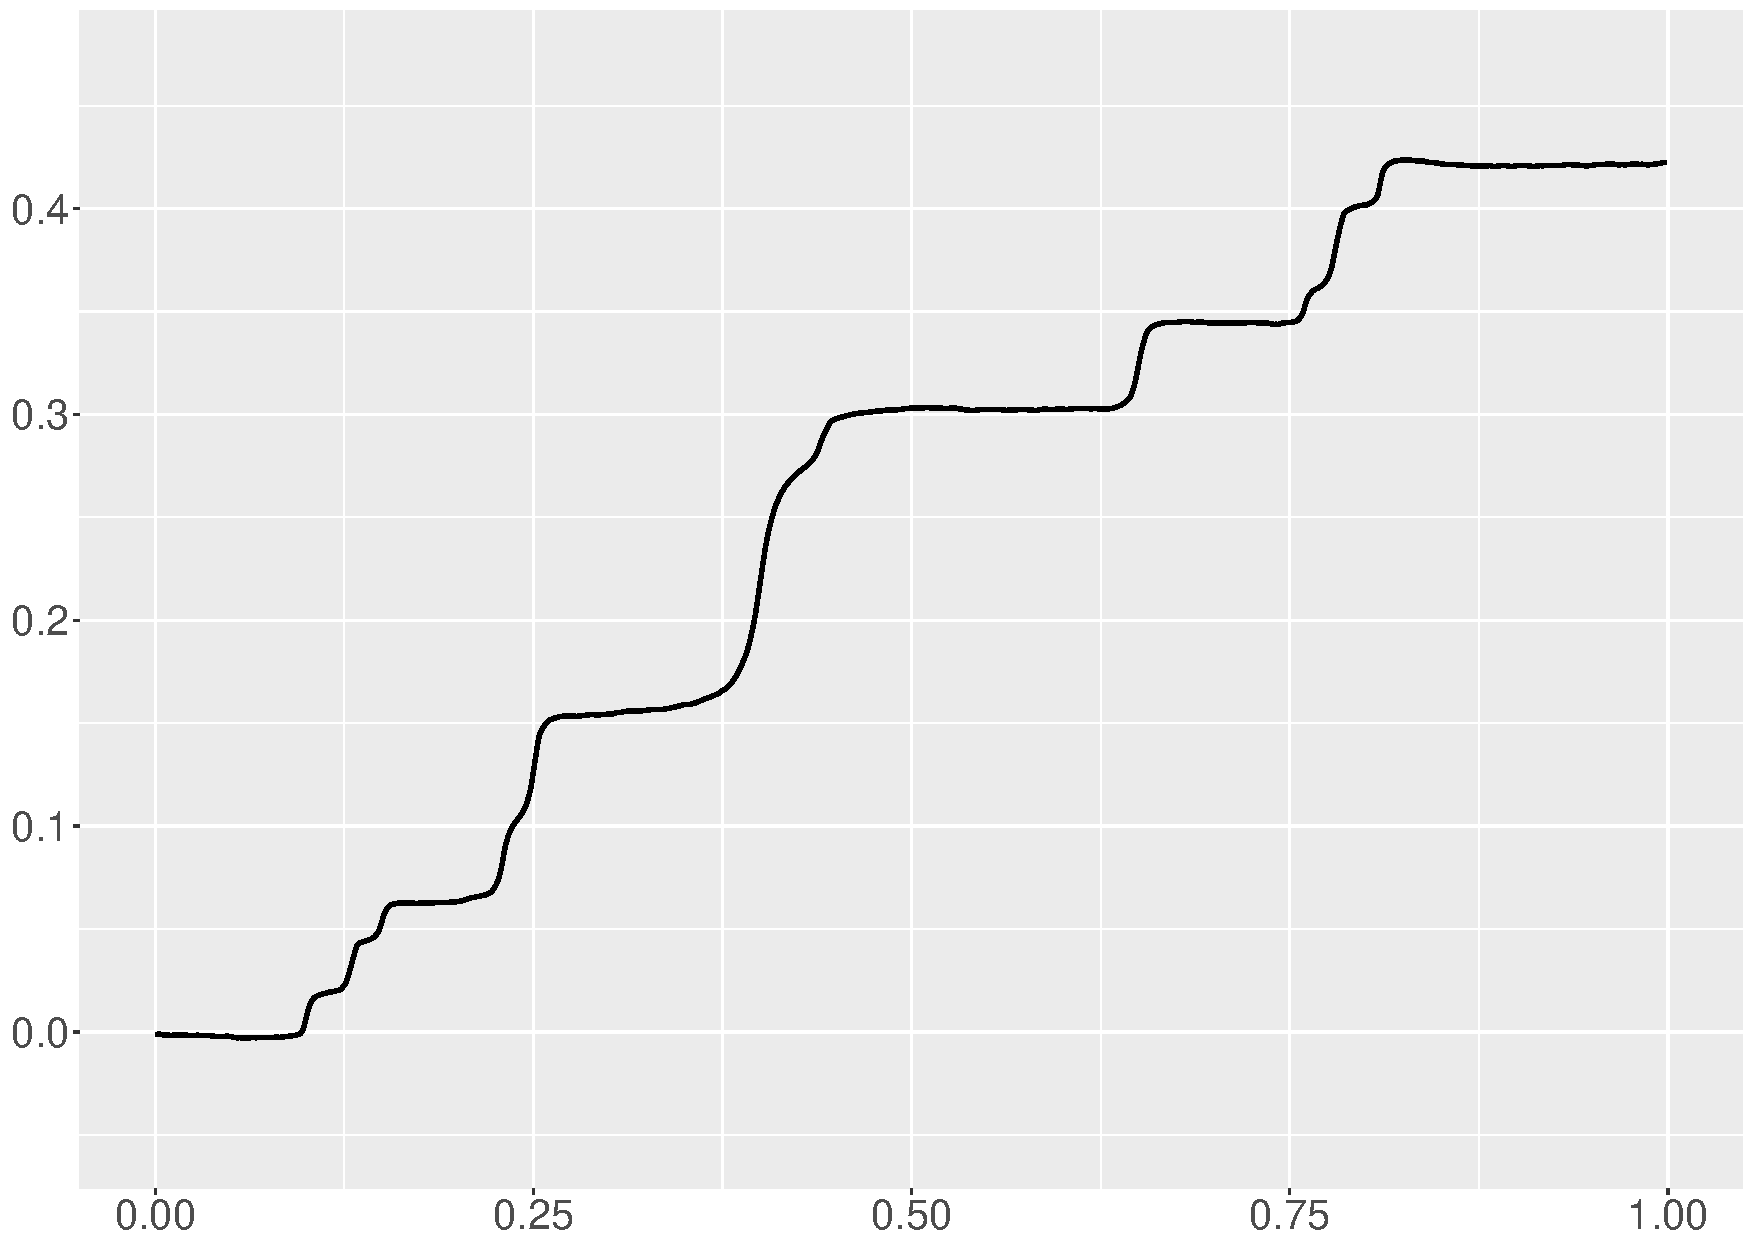
\includegraphics[width=\linewidth,height=0.45\textwidth]{Chapters/02TractorSplineTheory/plot/ggplot/ggBumpsTractor.pdf}
    \caption{Reconstruction by the proposed V-spline}
    \end{subfigure}
\caption{Numerical example: $\textit{Bumps}$. Comparison of different reconstruction methods with simulated data.}\label{num2}
 \end{figure}



%\begin{figure}
%  \centering
%    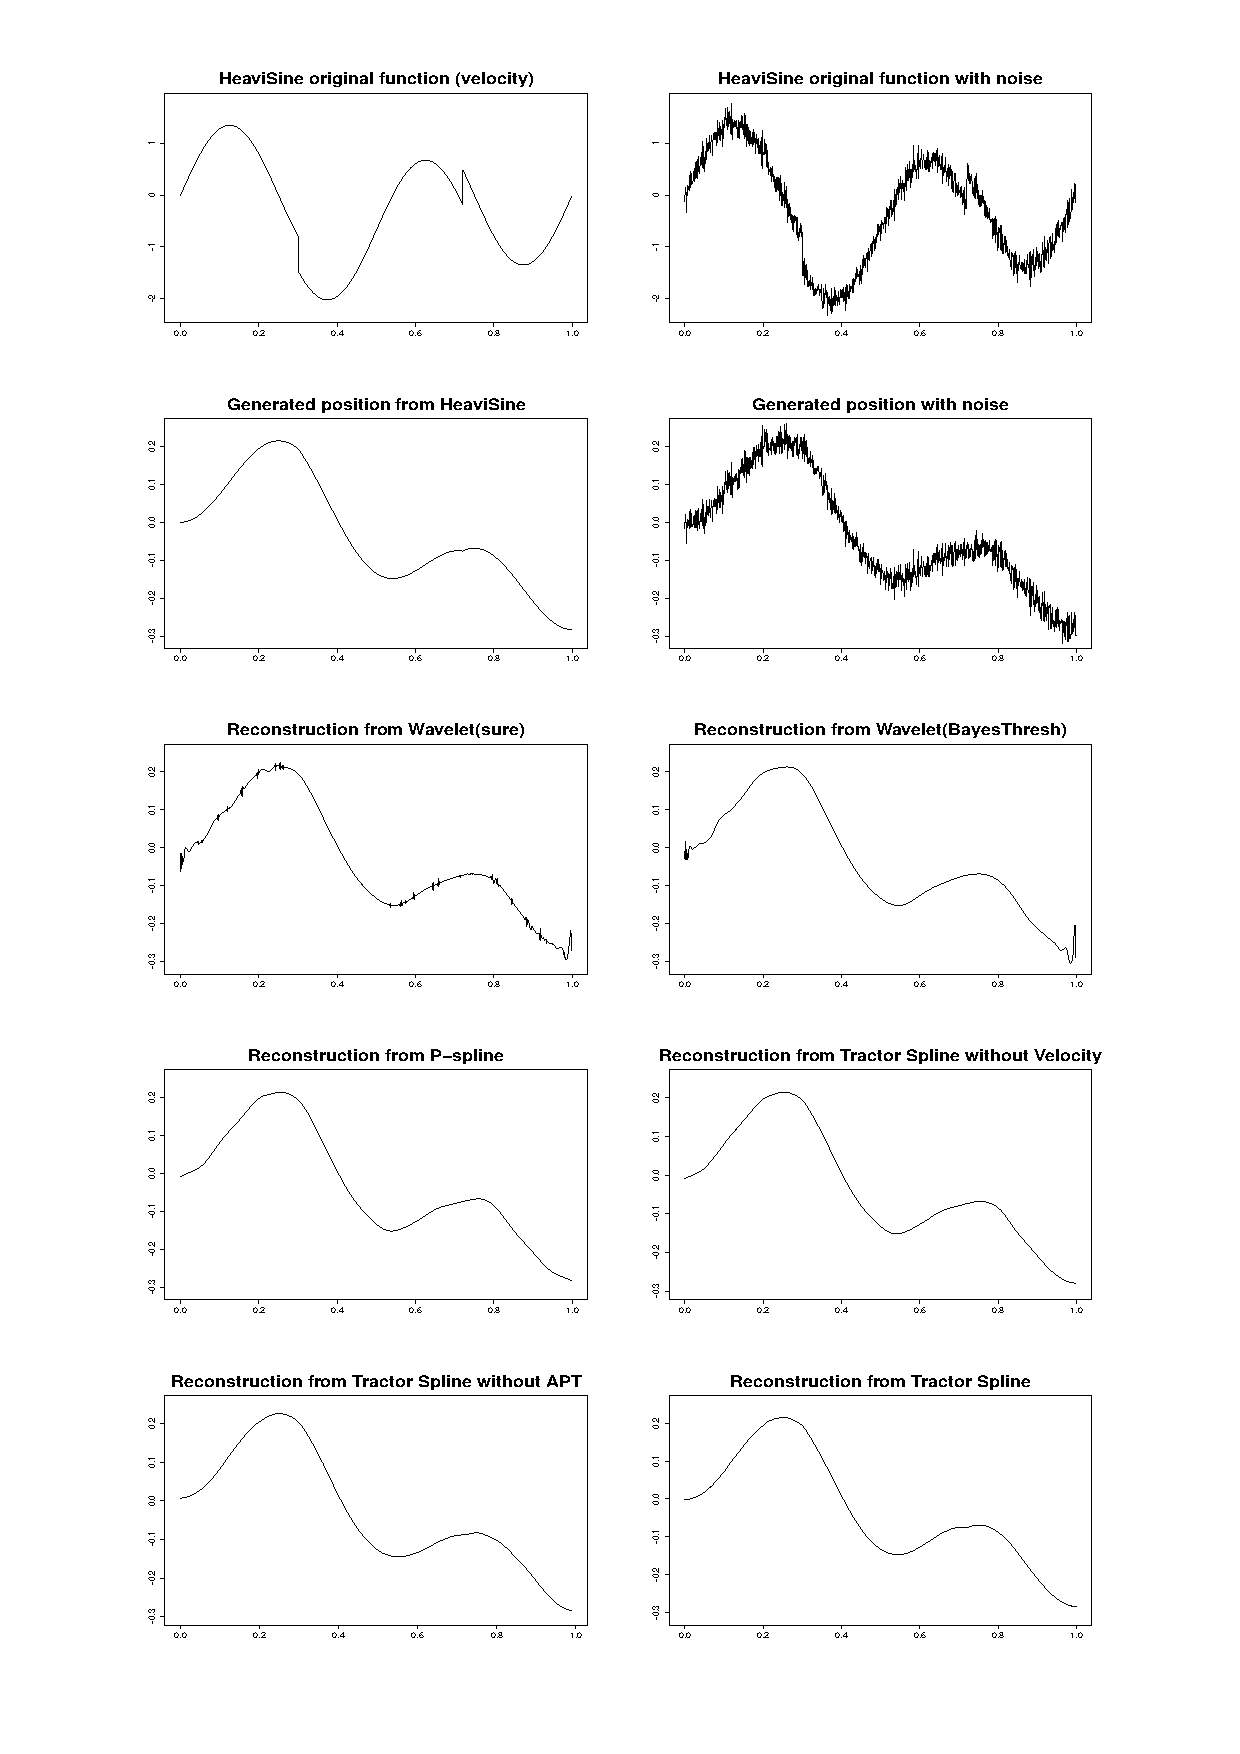
\includegraphics[width=\textwidth,height=14cm]{Chapters/02TractorSplineTheory/plot/heavi10} 
%  \caption{Numerical example: $\textit{HeaviSine}$. (a) The true velocity function. (b) Velocity with Gaussian noise at SNR=7. (c) Generated position function. (d) Position with Gaussian noise at SNR=7. (e) Reconstruction from Wavelet with sure threshold. (f) Reconstruction from Wavelet with BayesThresh approach. (g) Reconstruction by P-spline. (h) Reconstruction by V-spline setting $\gamma=0$. (i) Reconstruction by V-spline with normal penalty term. (j) Reconstruction by proposed V-spline.}\label{num3}
%\end{figure}



\begin{figure}
    \centering
    \begin{subfigure}{0.45\textwidth}
    \centering
    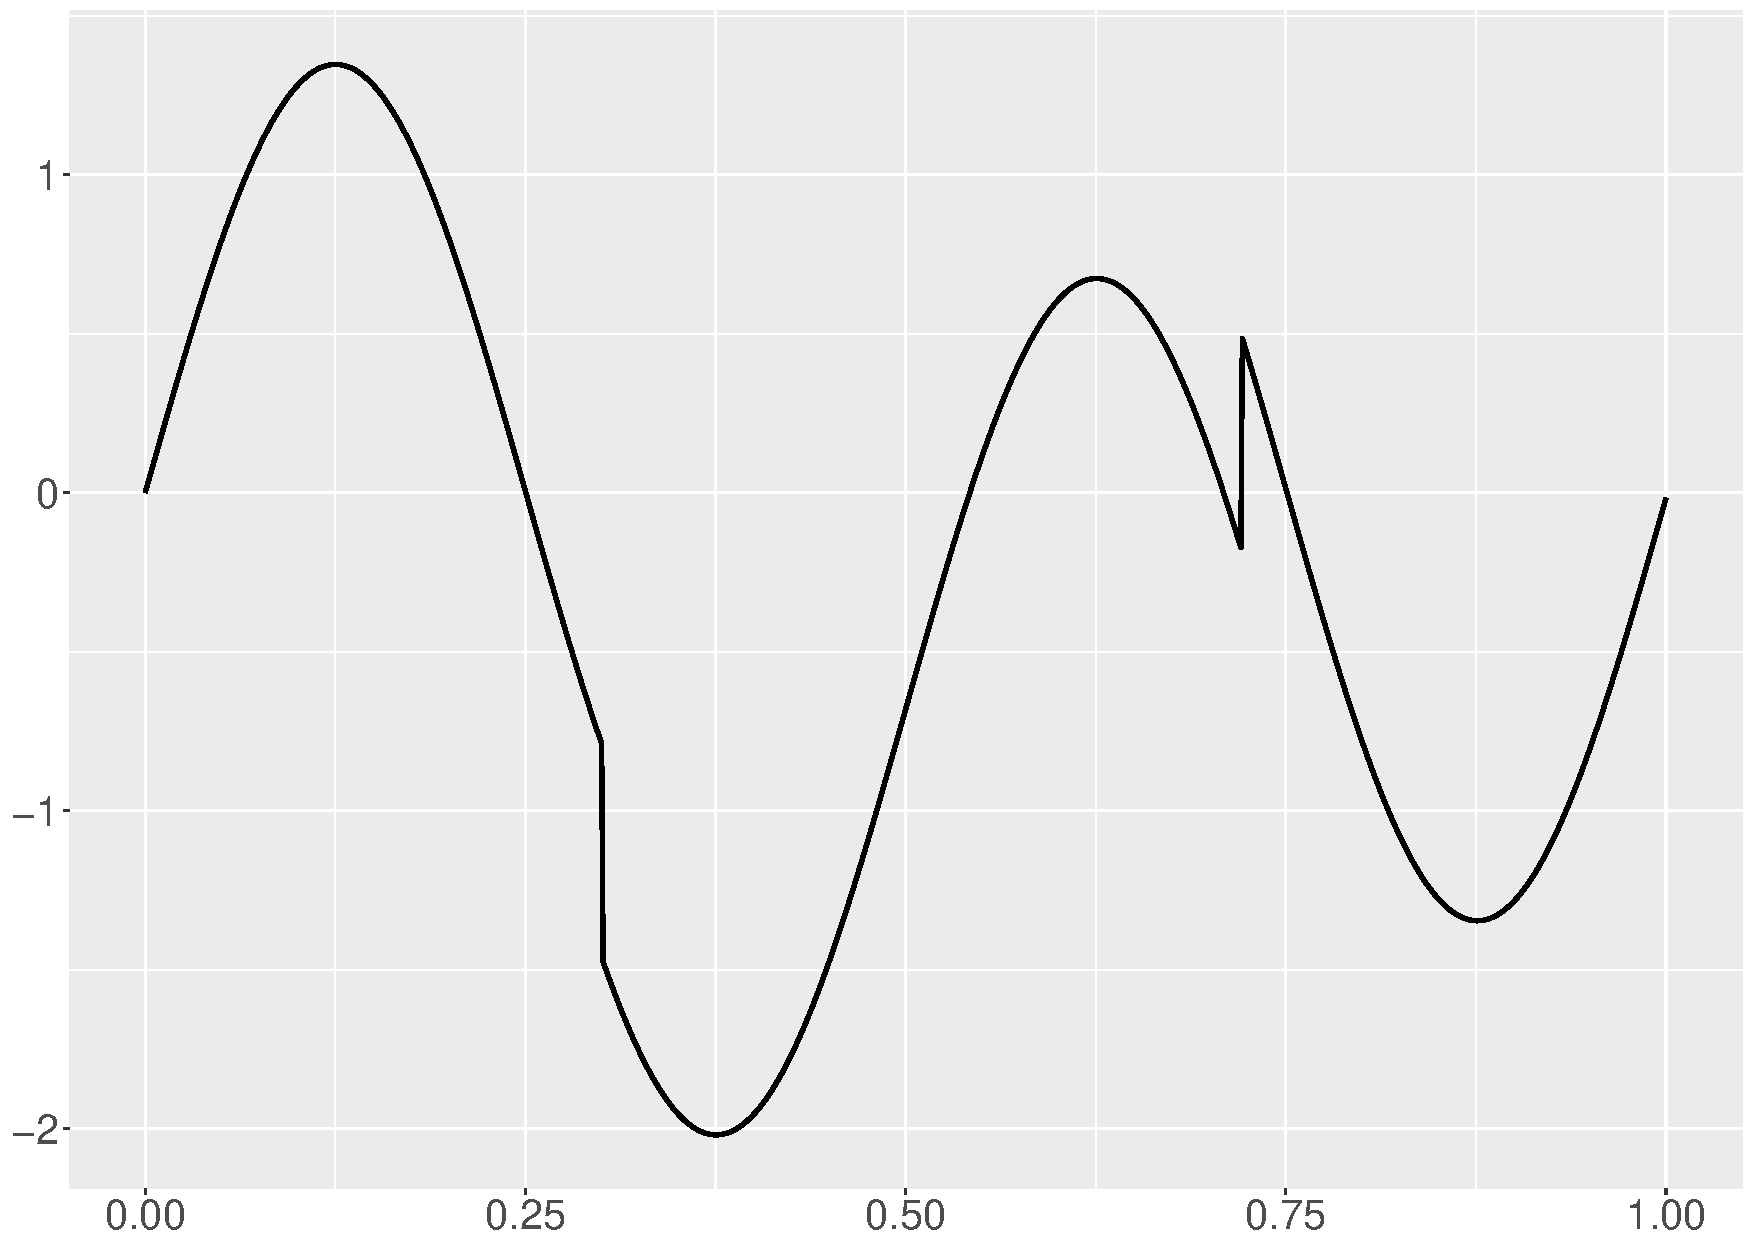
\includegraphics[width=\linewidth,height=0.45\textwidth]{Chapters/02TractorSplineTheory/plot/ggplot/ggHeaviSine.pdf}
    \caption{True \textit{HeaviSine} function}
    \end{subfigure}%
    \begin{subfigure}{0.45\textwidth}
    \centering
    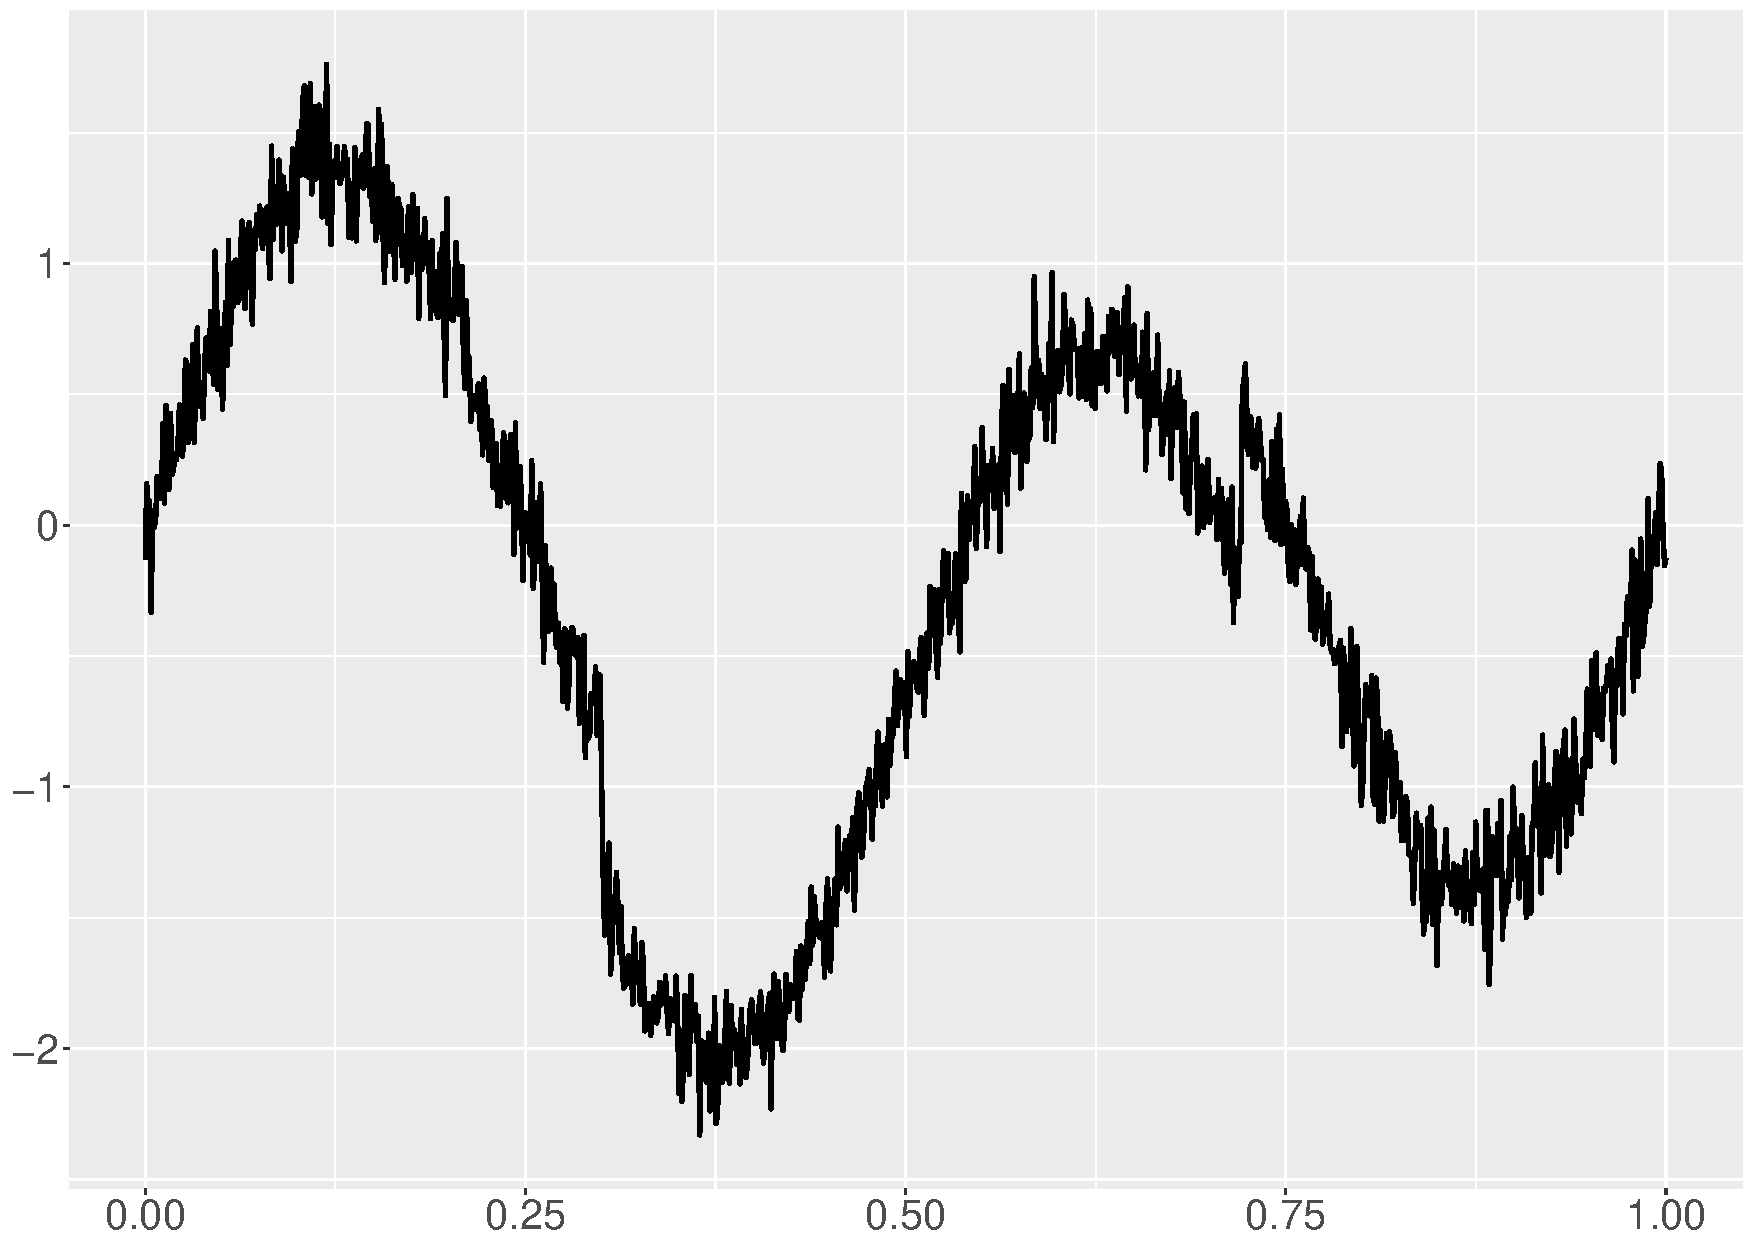
\includegraphics[width=\linewidth,height=0.45\textwidth]{Chapters/02TractorSplineTheory/plot/ggplot/ggHeaviSineNoise.pdf}
    \caption{Noisy \textit{HeaviSine} at \textit{SNR}=7}
    \end{subfigure}
    \begin{subfigure}{0.45\textwidth}
    \centering
    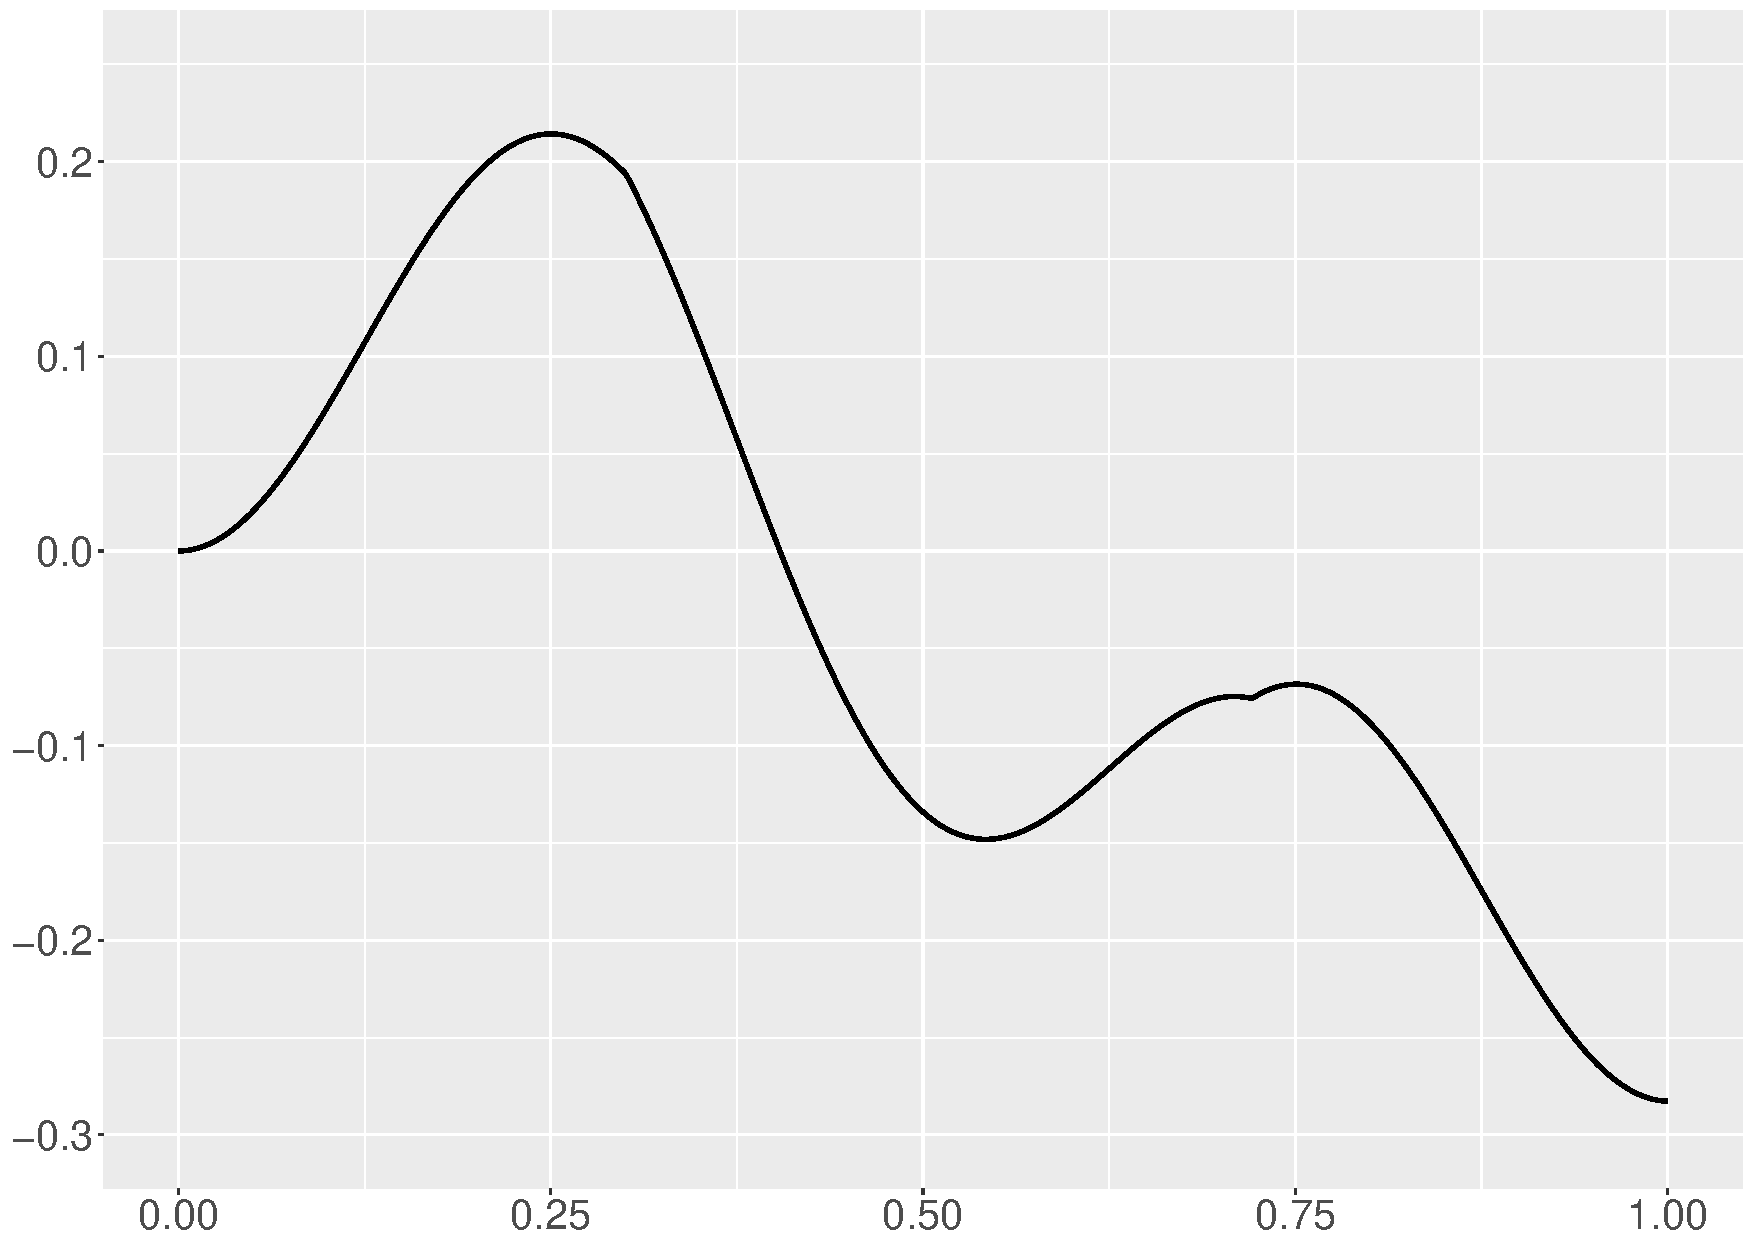
\includegraphics[width=\linewidth,height=0.45\textwidth]{Chapters/02TractorSplineTheory/plot/ggplot/ggHeaviSinePosition.pdf}
    \caption{Generated positions}
    \end{subfigure}
    \begin{subfigure}{0.45\textwidth}
    \centering
    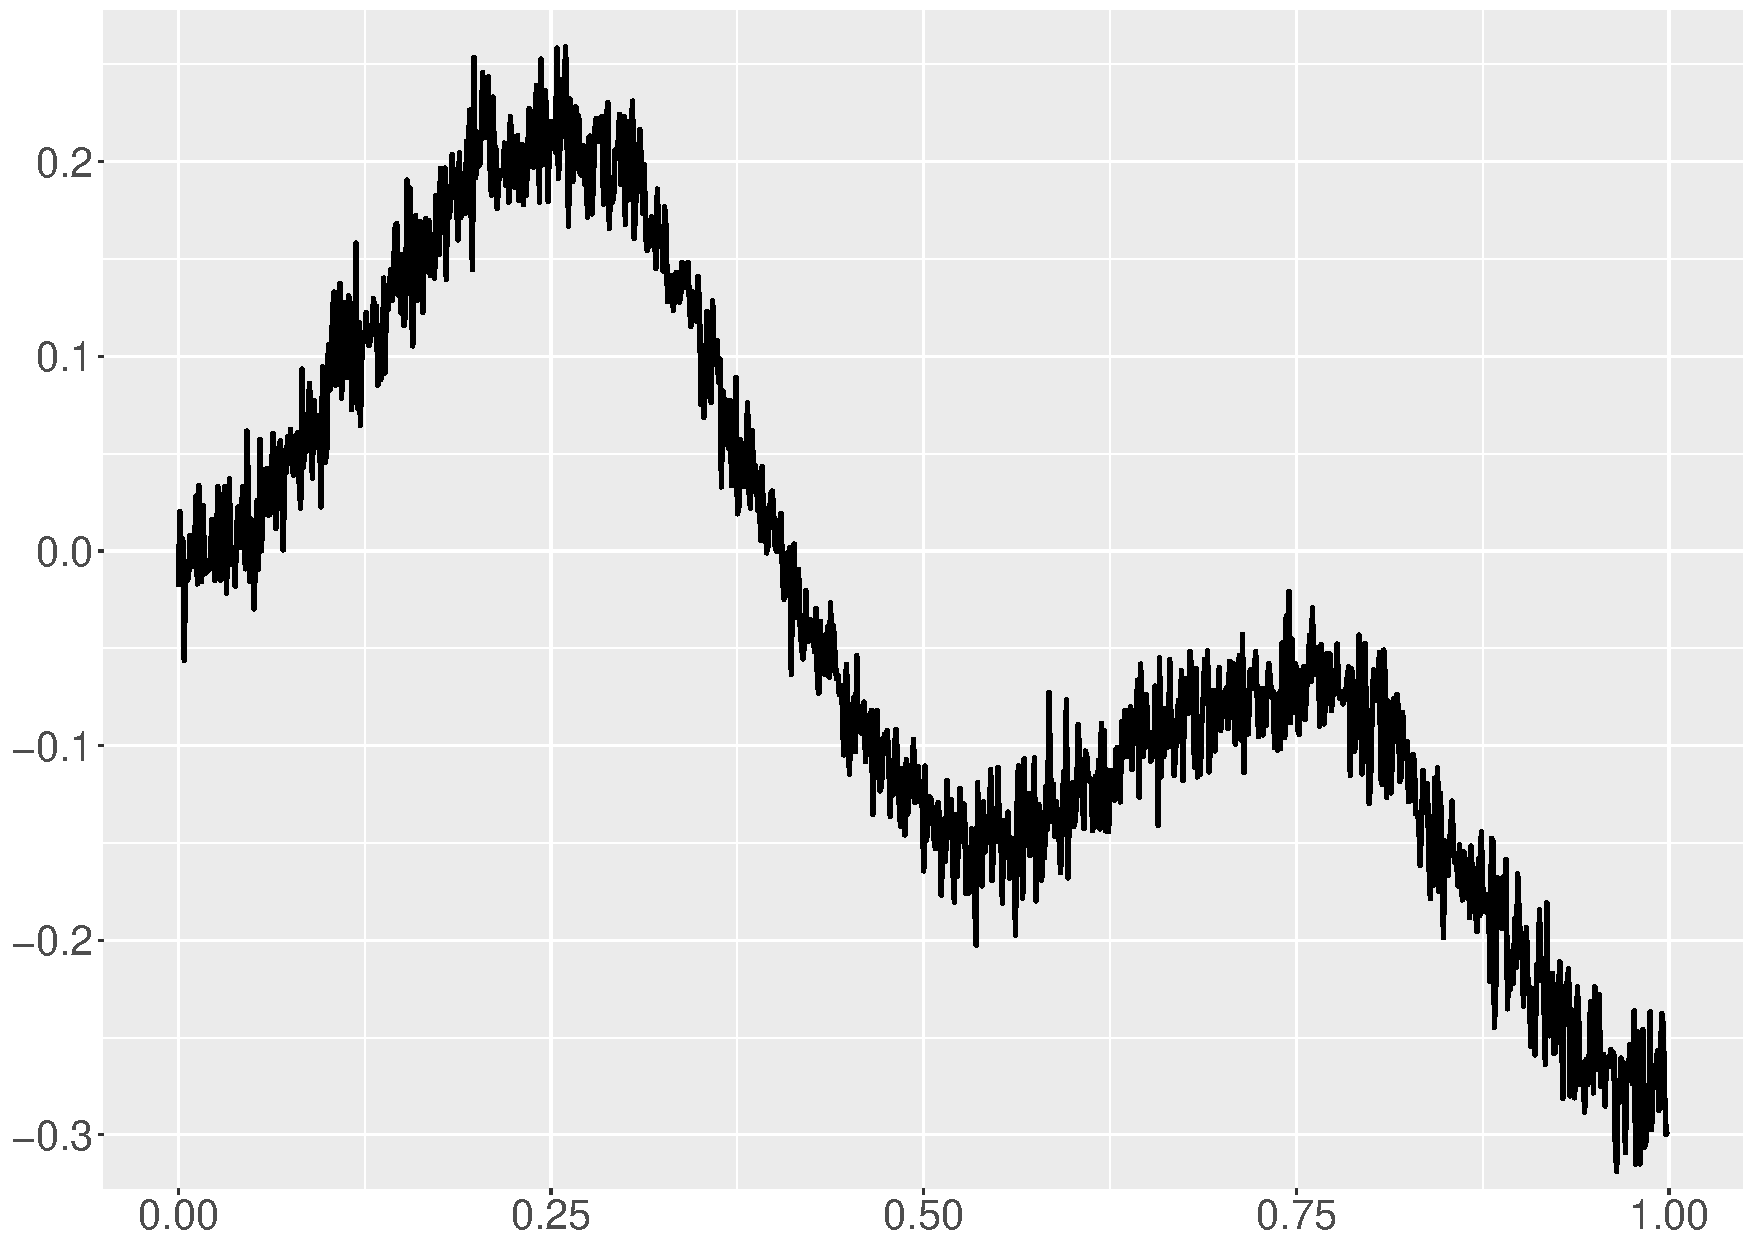
\includegraphics[width=\linewidth,height=0.45\textwidth]{Chapters/02TractorSplineTheory/plot/ggplot/ggHeaviSinePositionNoise.pdf}
    \caption{Noisy position at \textit{SNR}=7}
    \end{subfigure}
    \begin{subfigure}{0.45\textwidth}
    \centering
    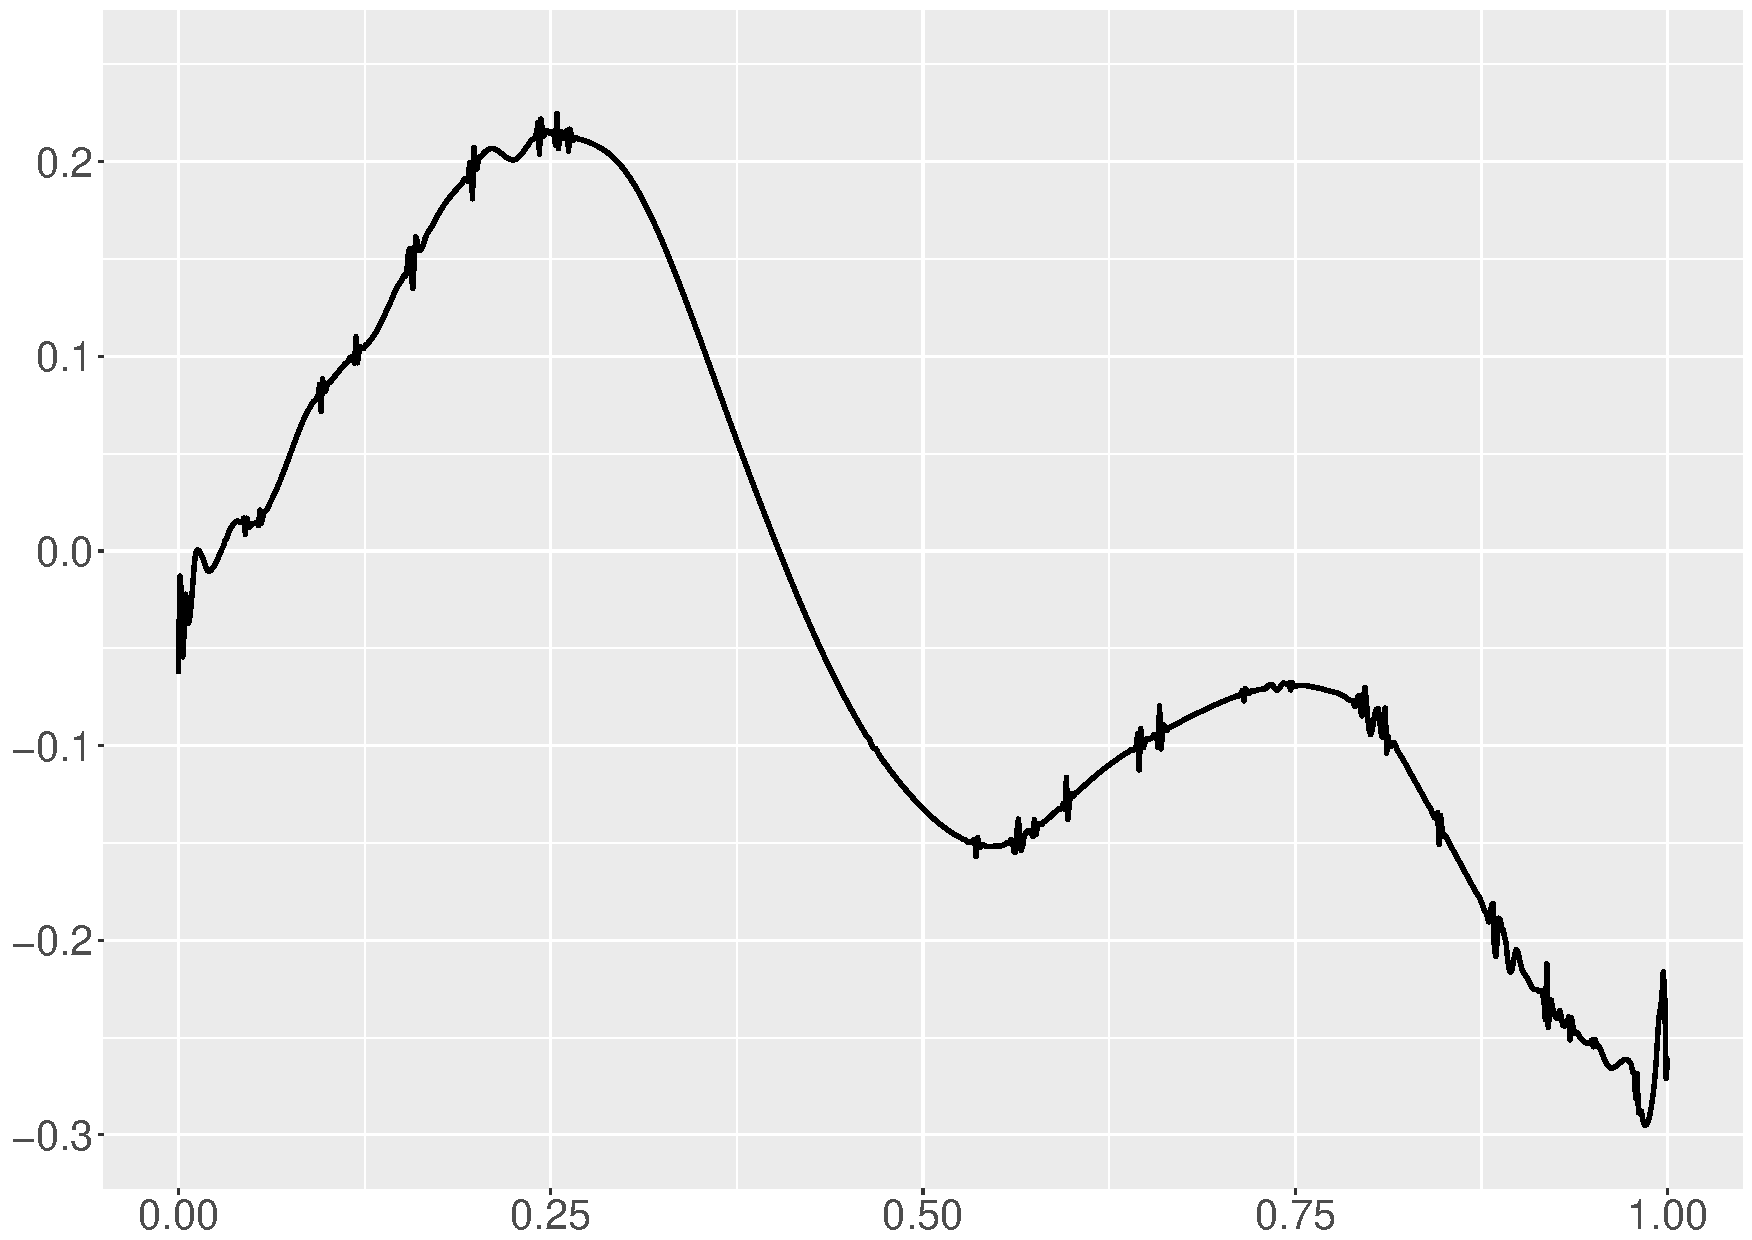
\includegraphics[width=\linewidth,height=0.45\textwidth]{Chapters/02TractorSplineTheory/plot/ggplot/ggHeaviSineSure.pdf}
    \caption{Reconstruction from Wavelet by sure threshold}
    \end{subfigure}
    \begin{subfigure}{0.45\textwidth}
    \centering
    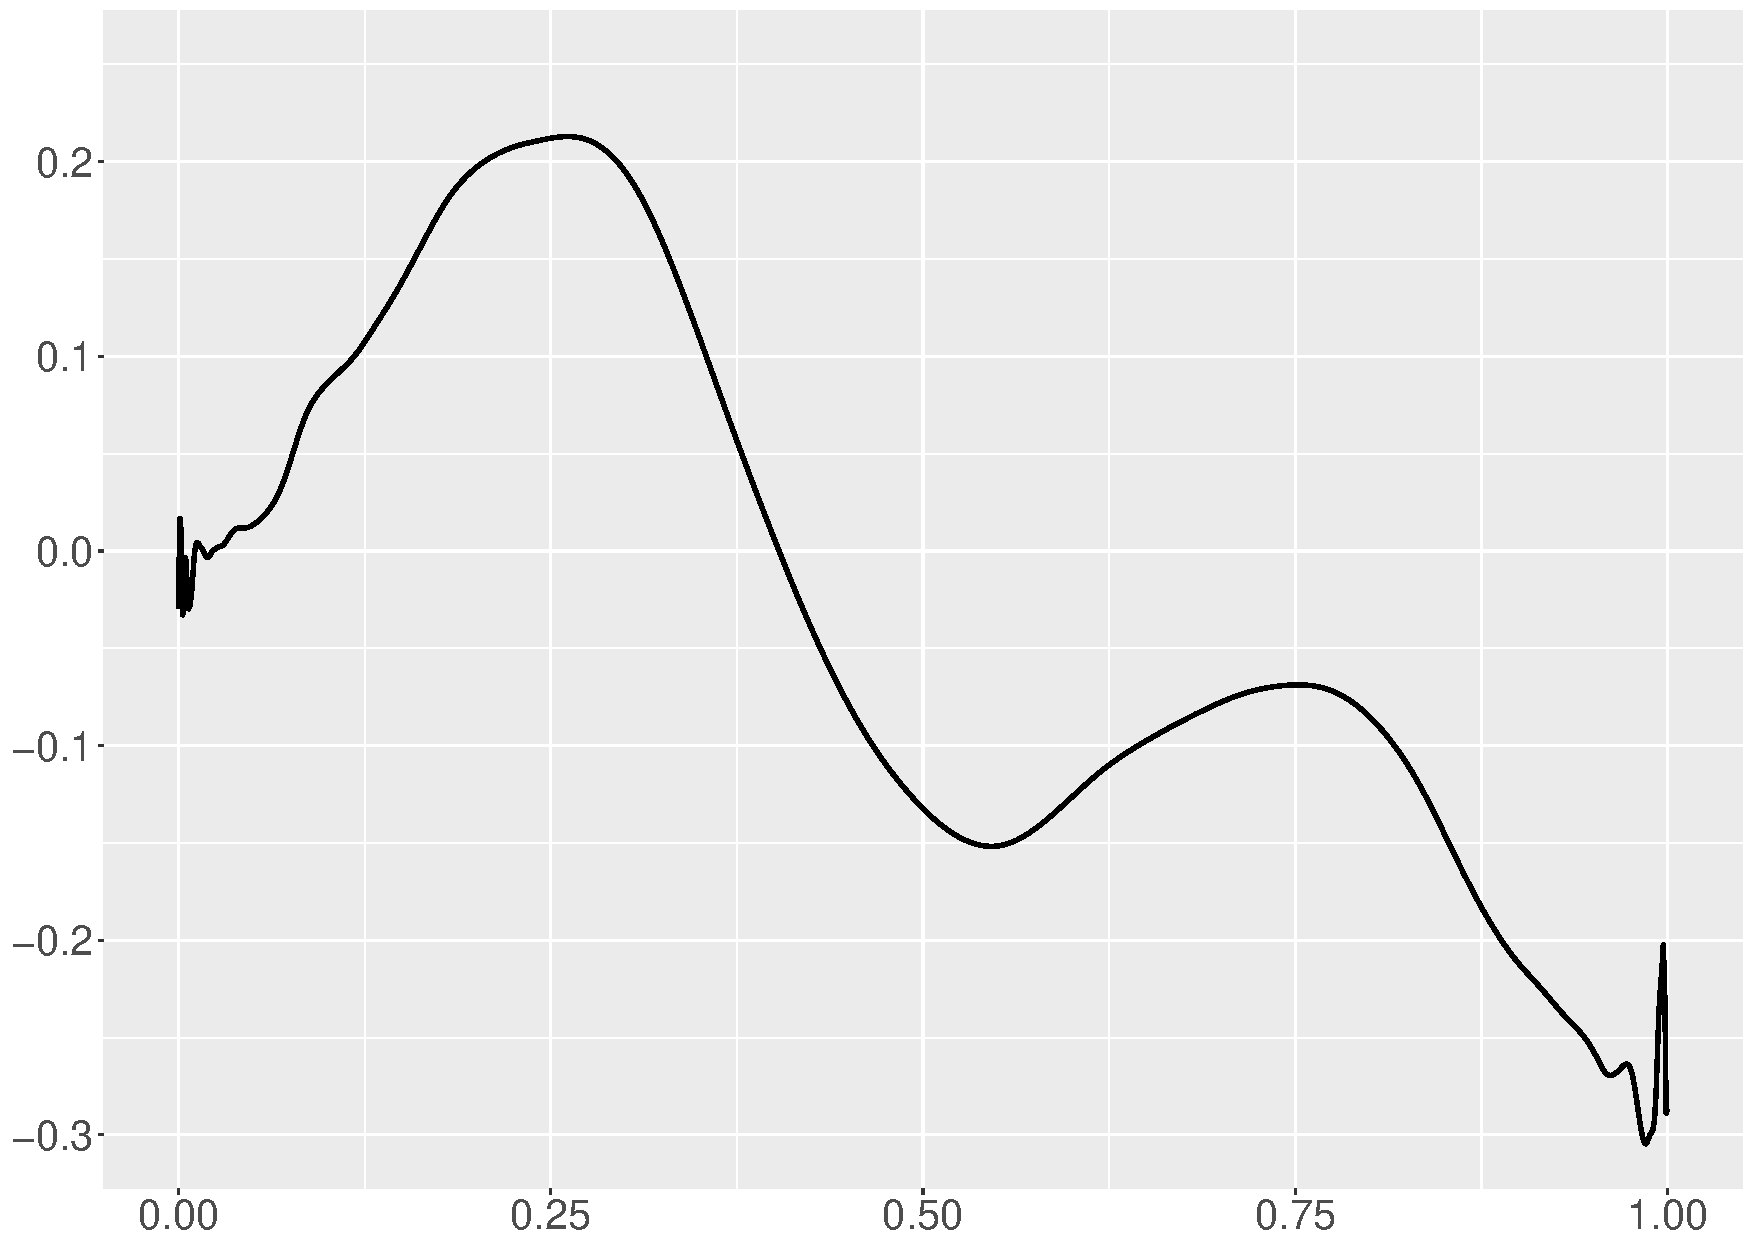
\includegraphics[width=\linewidth,height=0.45\textwidth]{Chapters/02TractorSplineTheory/plot/ggplot/ggHeaviSineBayes.pdf}
    \caption{Reconstruction from Wavelet by BayesThresh approach}
    \end{subfigure}
    \begin{subfigure}{0.45\textwidth}
    \centering
    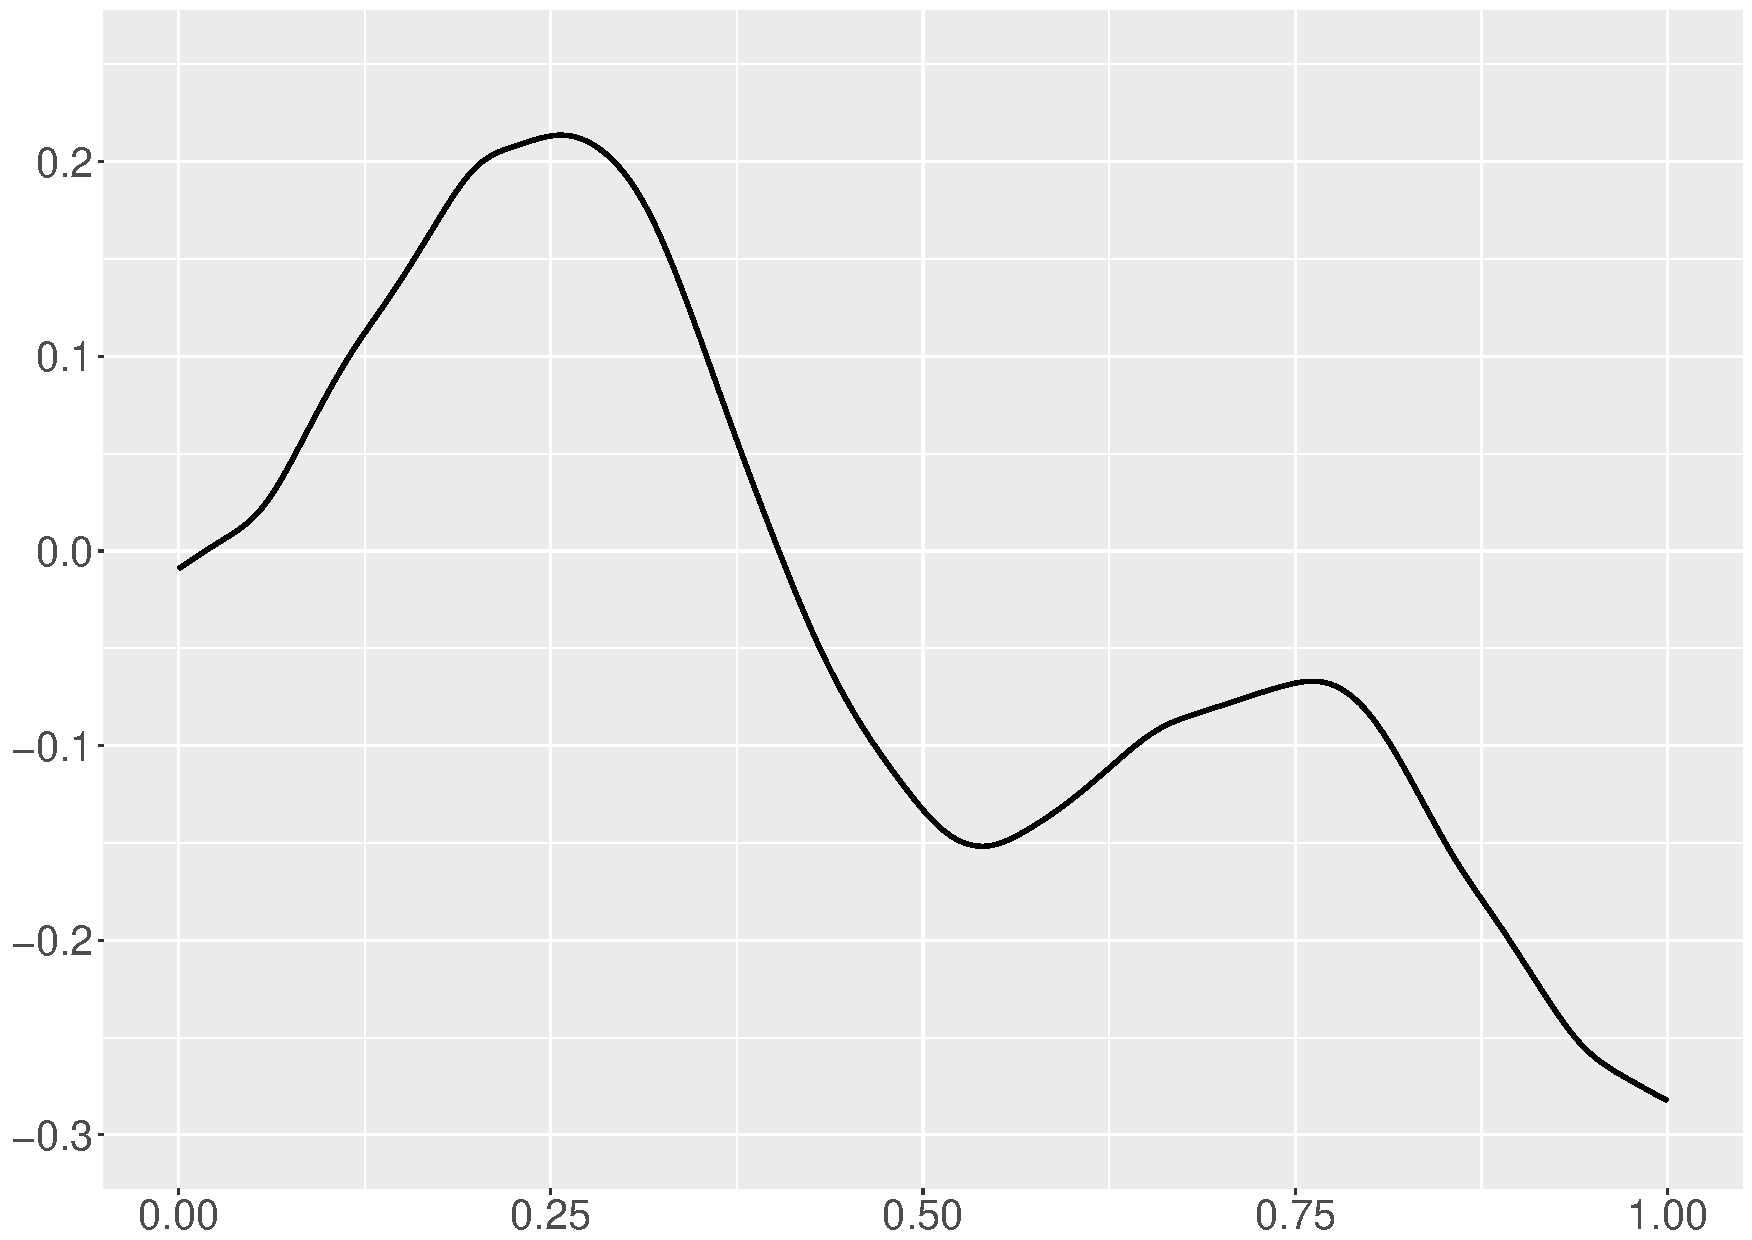
\includegraphics[width=\linewidth,height=0.45\textwidth]{Chapters/02TractorSplineTheory/plot/ggplot/ggHeaviSinePSpline.pdf}
    \caption{Reconstruction by P-spline \\\mbox{  } }
    \end{subfigure}
    \begin{subfigure}{0.45\textwidth}
    \centering
    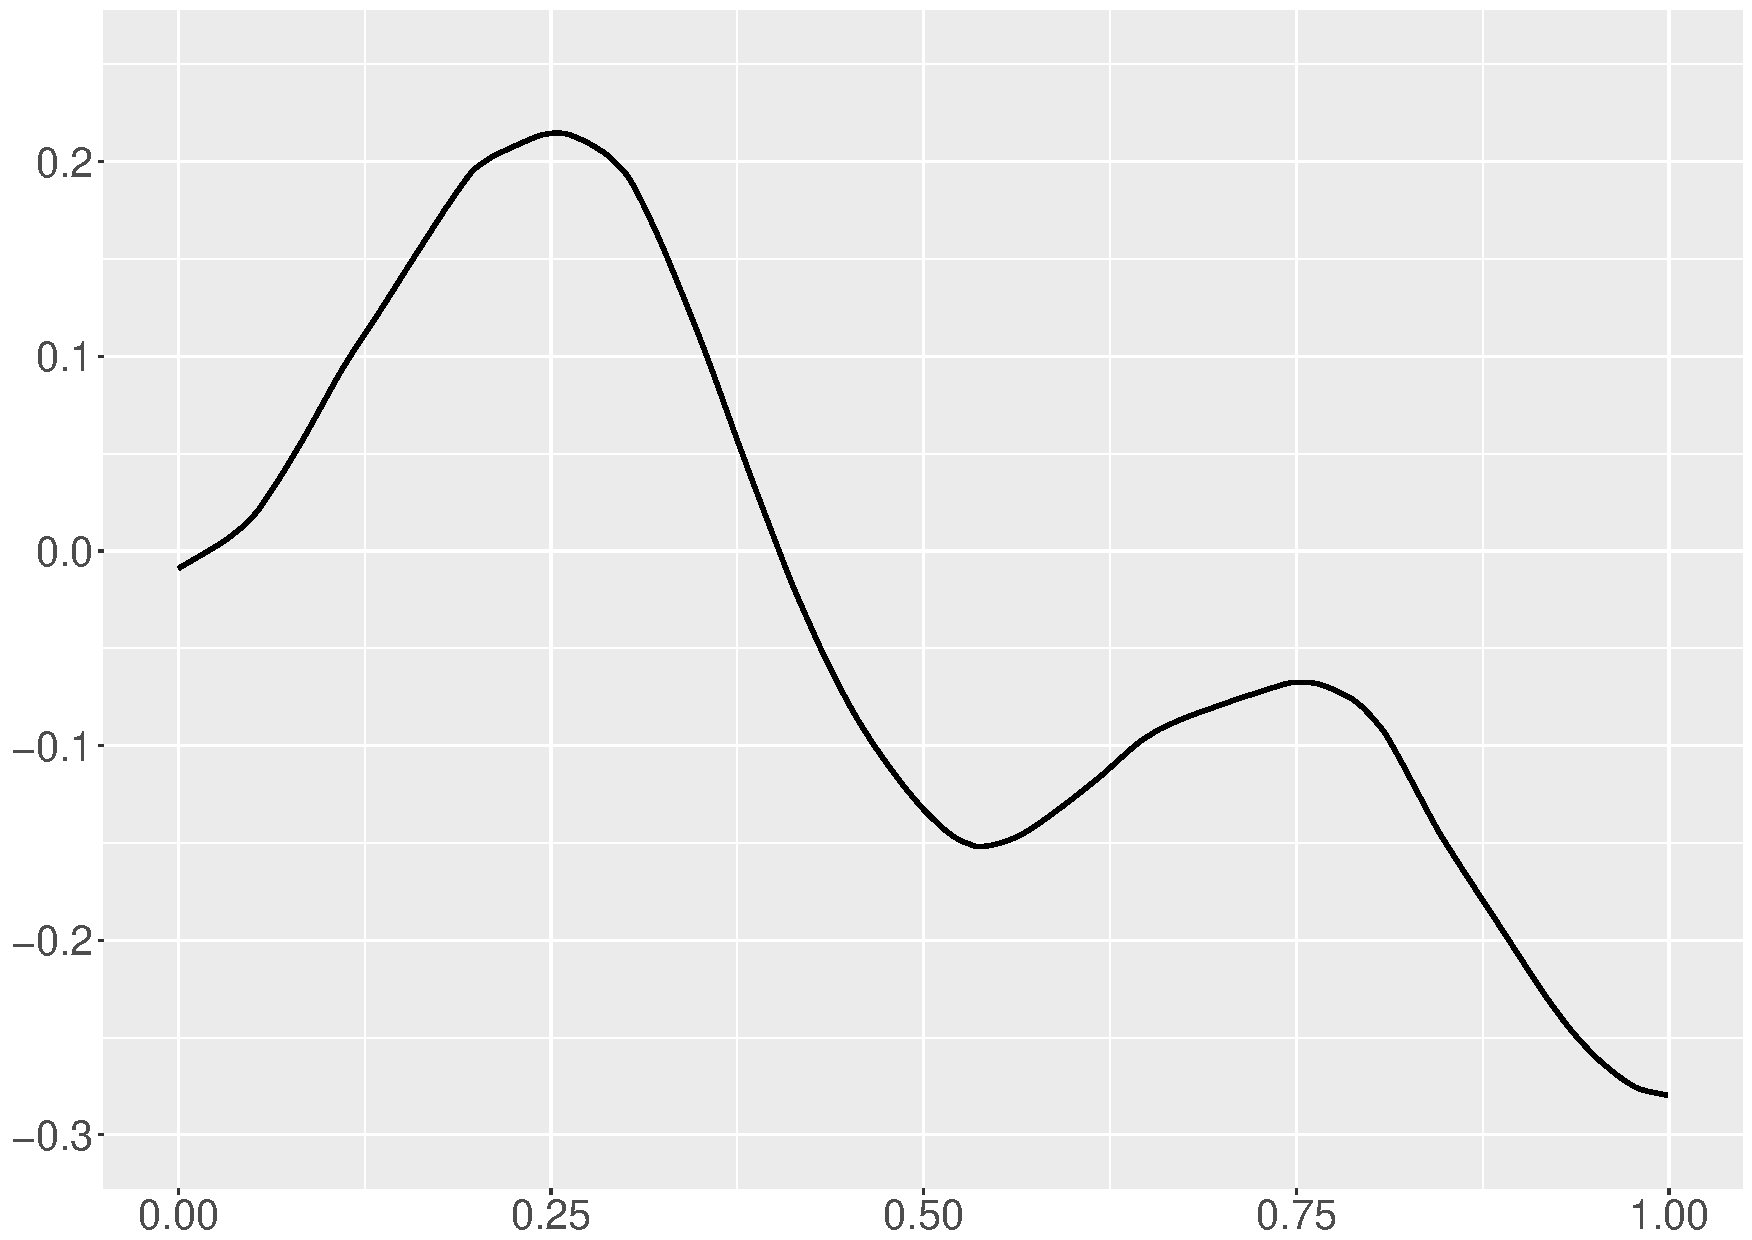
\includegraphics[width=\linewidth,height=0.45\textwidth]{Chapters/02TractorSplineTheory/plot/ggplot/ggHeaviSineGamma.pdf}
    \caption{Reconstruction by V-spline setting $\gamma=0$}
    \end{subfigure}
  \begin{subfigure}{0.45\textwidth}
    \centering
    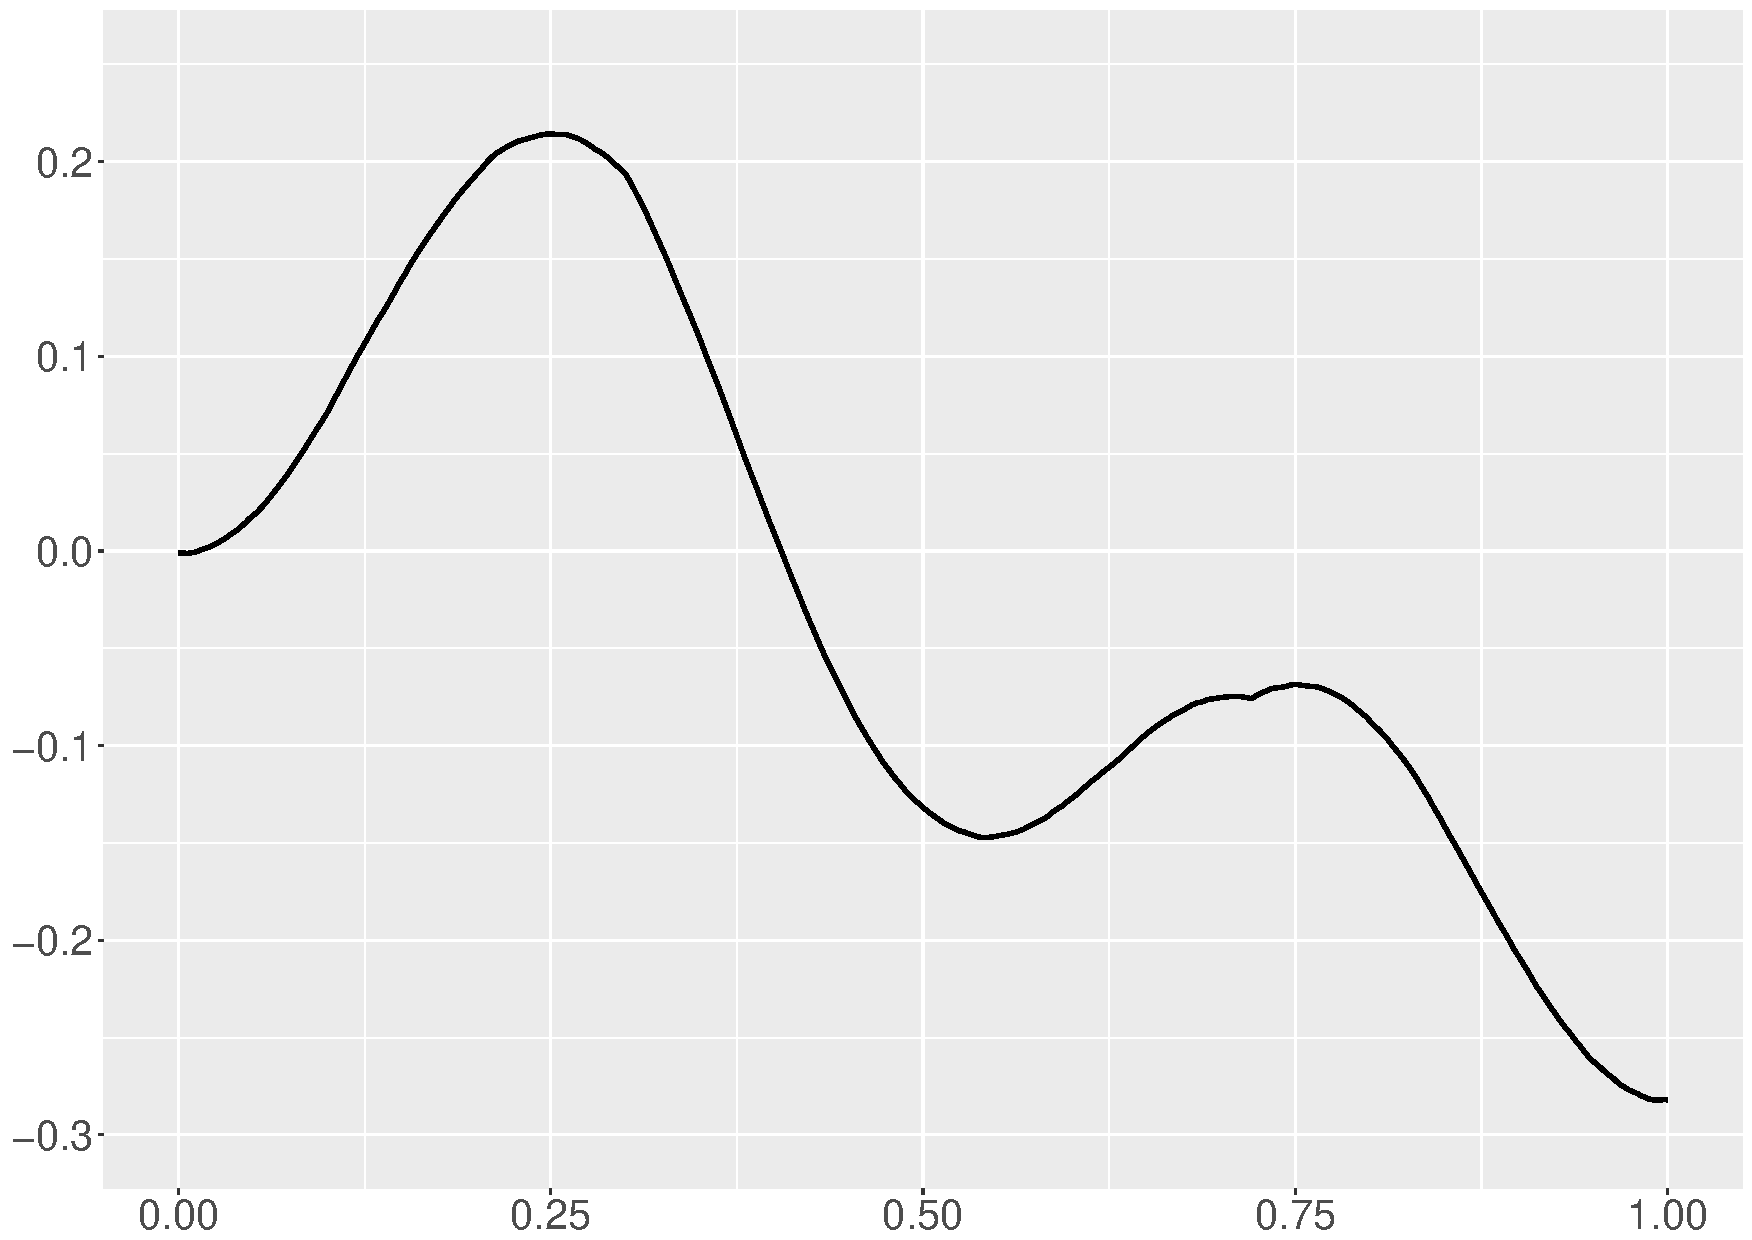
\includegraphics[width=\linewidth,height=0.45\textwidth]{Chapters/02TractorSplineTheory/plot/ggplot/ggHeaviSineTractorAPT.pdf}
    \caption{Reconstruction by V-spline with conventional penalty term}
    \end{subfigure}
    \begin{subfigure}{0.45\textwidth}
    \centering
    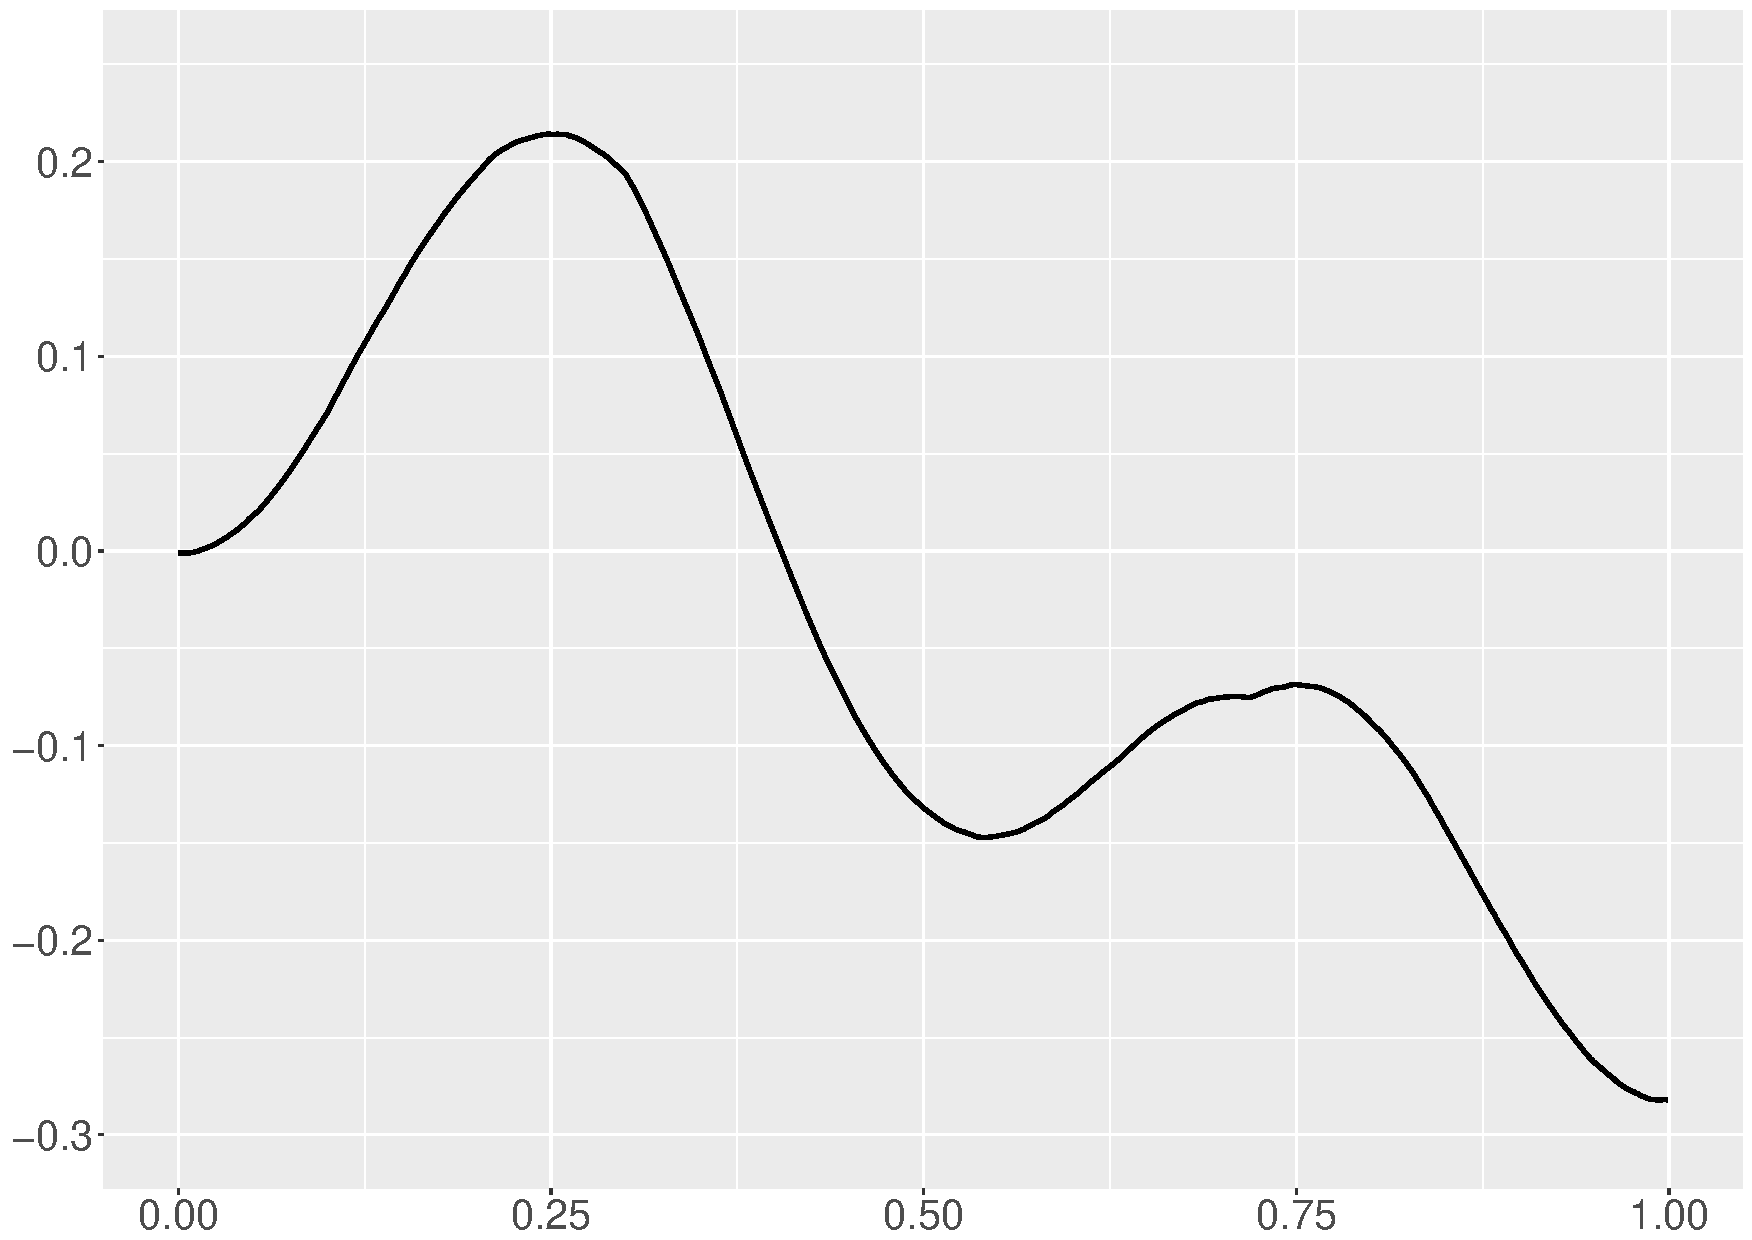
\includegraphics[width=\linewidth,height=0.45\textwidth]{Chapters/02TractorSplineTheory/plot/ggplot/ggHeaviSineTractor.pdf}
    \caption{Reconstruction by the proposed V-spline}
    \end{subfigure}
\caption{Numerical example: $\textit{HeaviSine}$. Comparison of different reconstruction methods with simulated data.}\label{num3}
 \end{figure}

%
%
%\begin{figure}
%  \centering
%         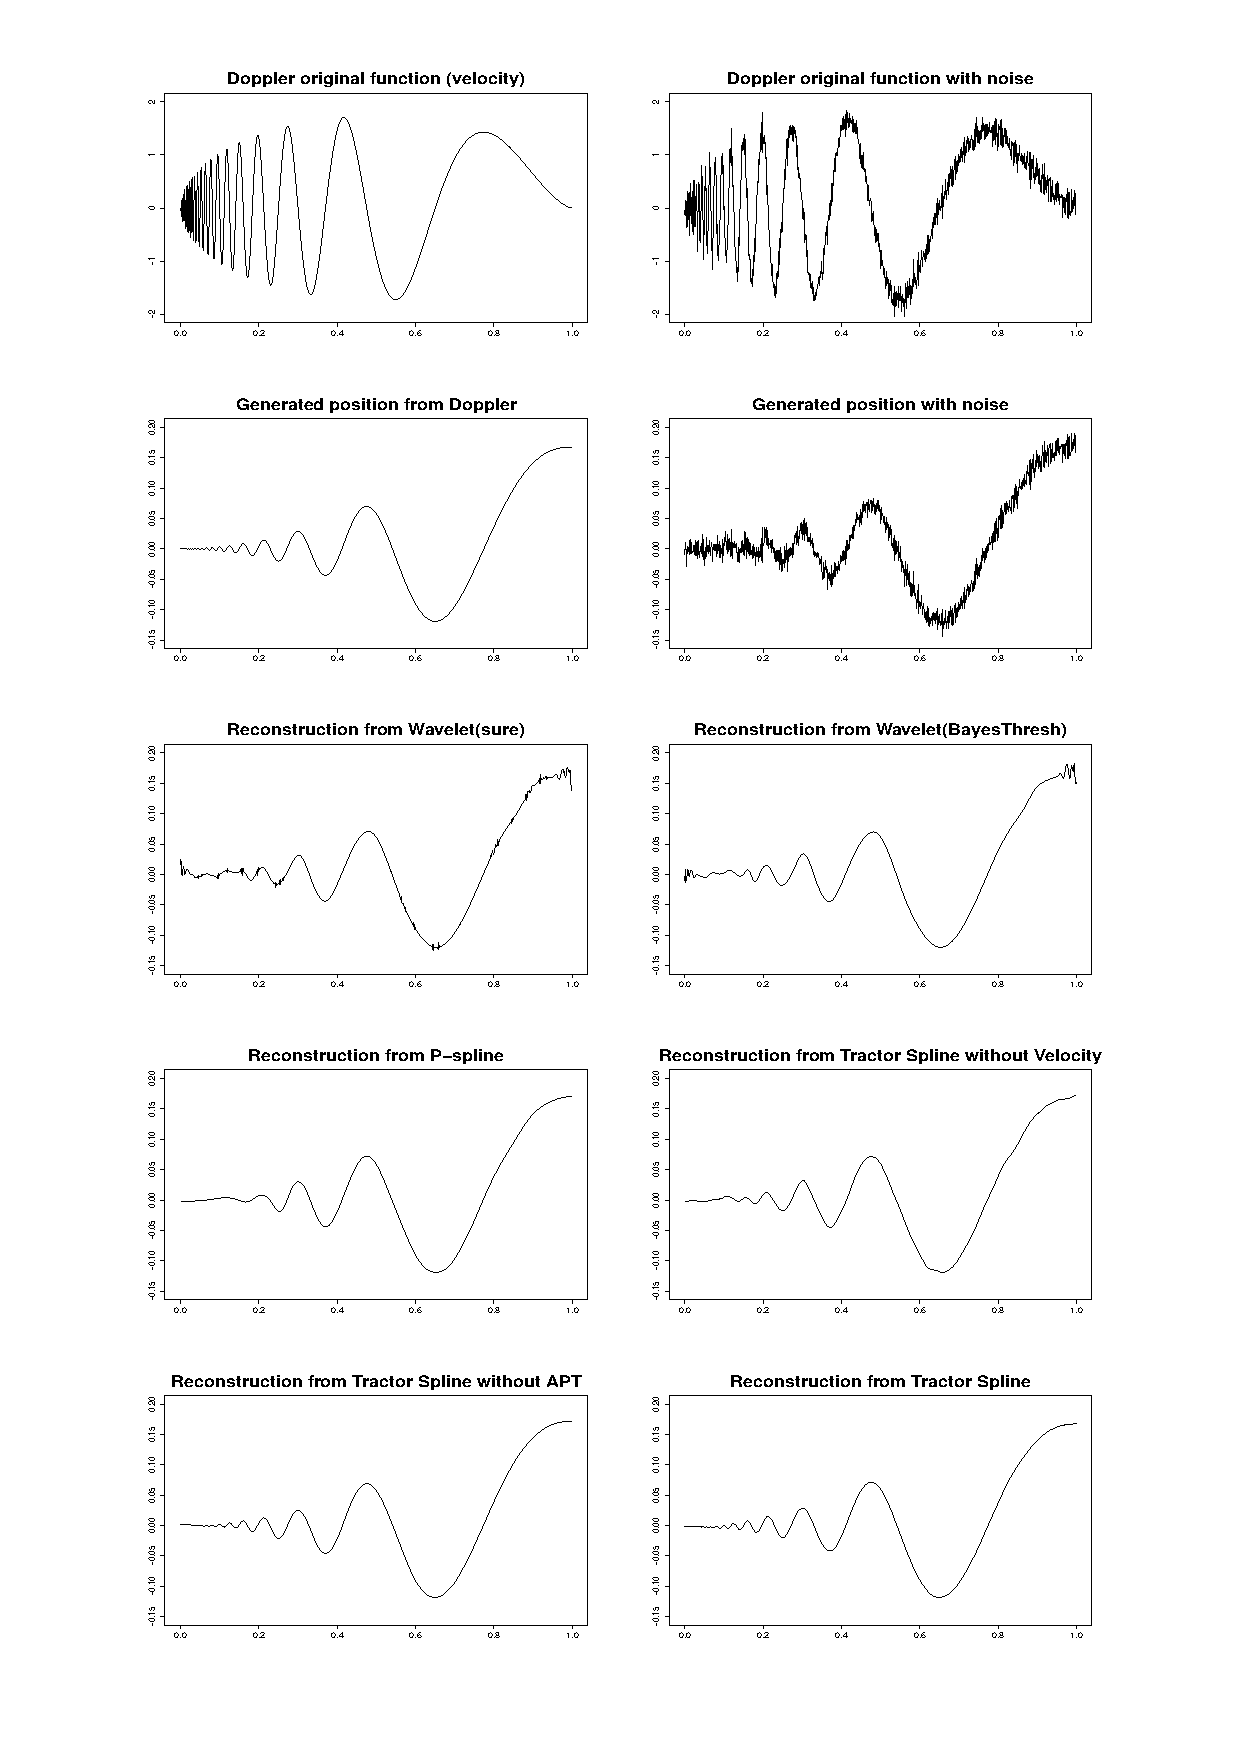
\includegraphics[width=\textwidth,height=14cm]{Chapters/02TractorSplineTheory/plot/doppler10} 
%  \caption{Numerical example: $\textit{Doppler}$. (a) The true velocity function. (b) Velocity with Gaussian noise at SNR=7. (c) Generated position function. (d) Position with Gaussian noise at SNR=7. (e) Reconstruction from Wavelet with sure threshold. (f) Reconstruction from Wavelet with BayesThresh approach. (g) Reconstruction by P-spline. (h) Reconstruction by V-spline setting $\gamma=0$. (i) Reconstruction by V-spline with normal penalty term. (j) Reconstruction by proposed V-spline.}\label{num4}
%\end{figure}


\begin{figure}
    \centering
    \begin{subfigure}{0.45\textwidth}
    \centering
    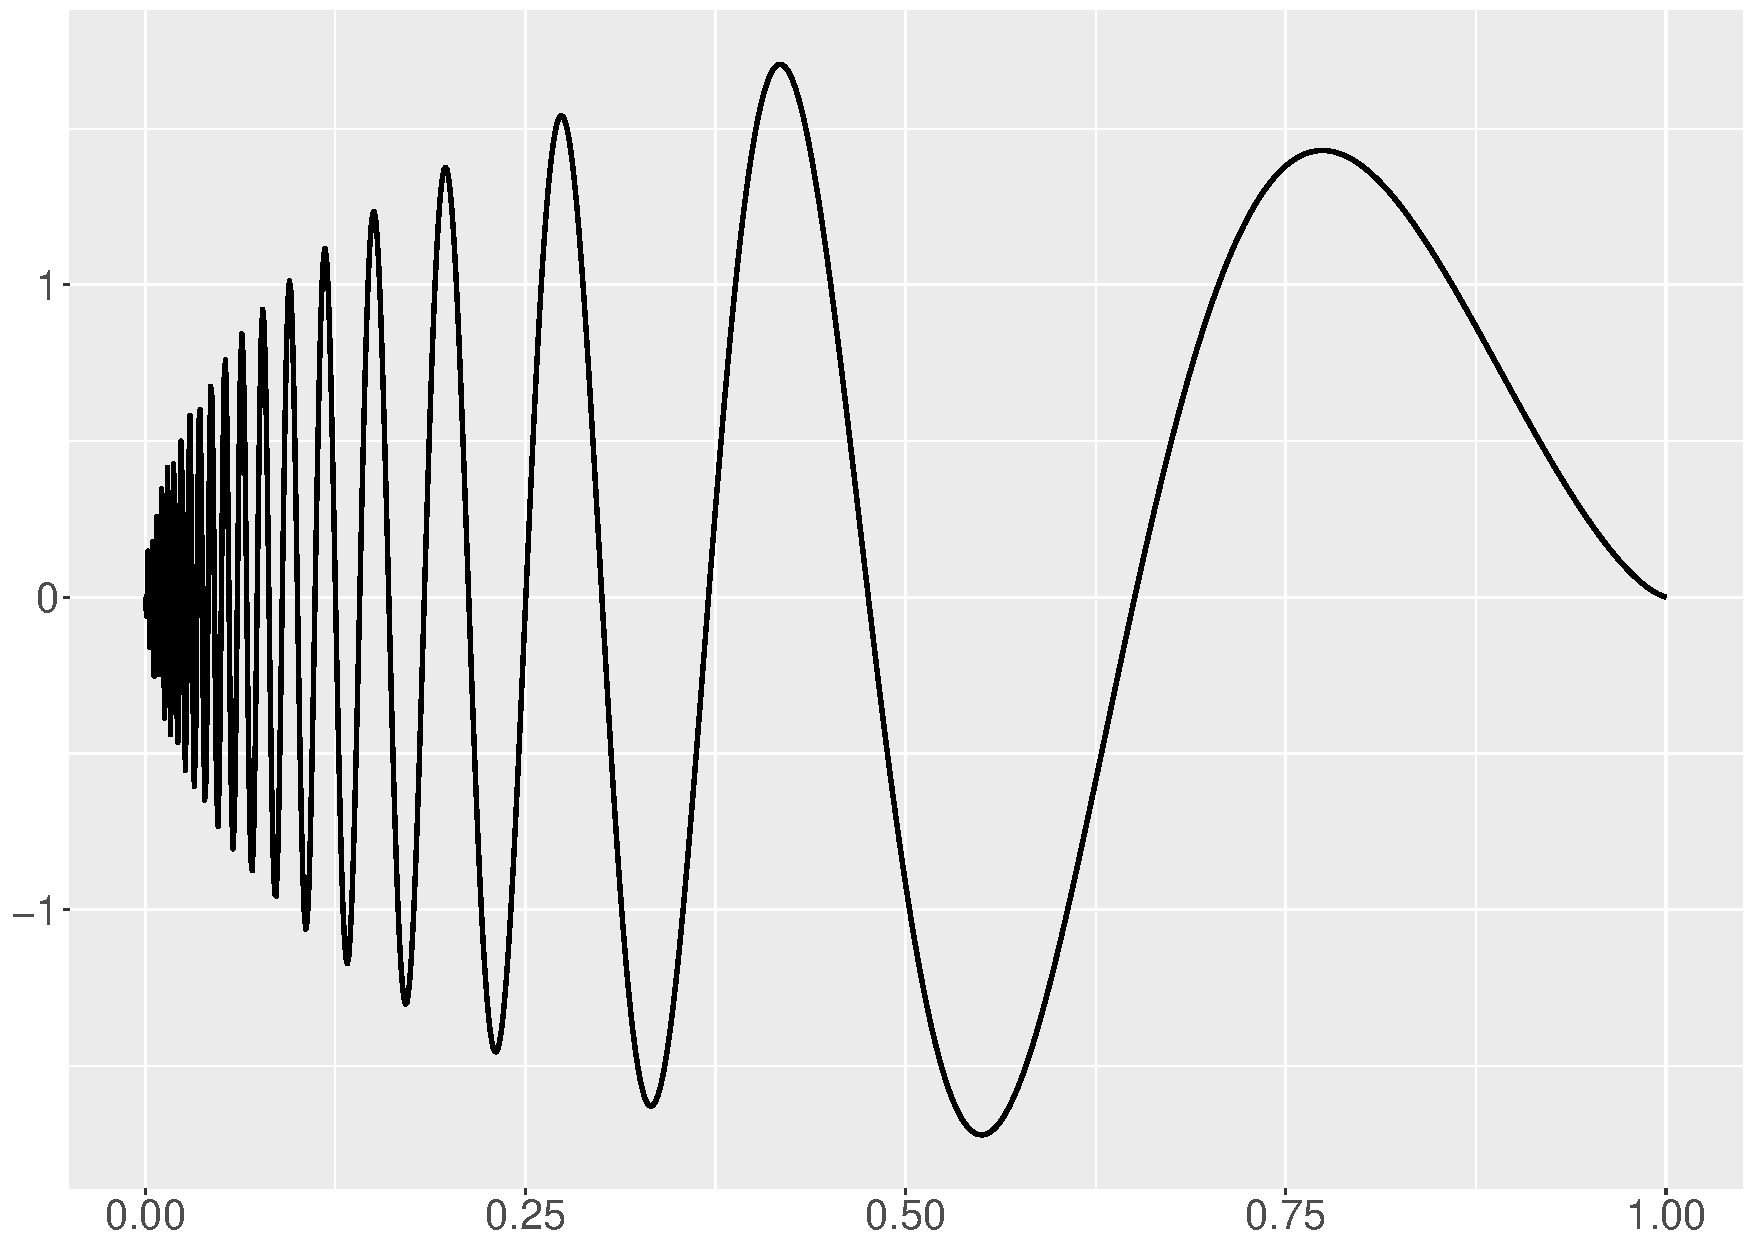
\includegraphics[width=\linewidth,height=0.45\textwidth]{Chapters/02TractorSplineTheory/plot/ggplot/ggDoppler.pdf}
    \caption{True \textit{Doppler} function}
    \end{subfigure}%
    \begin{subfigure}{0.45\textwidth}
    \centering
    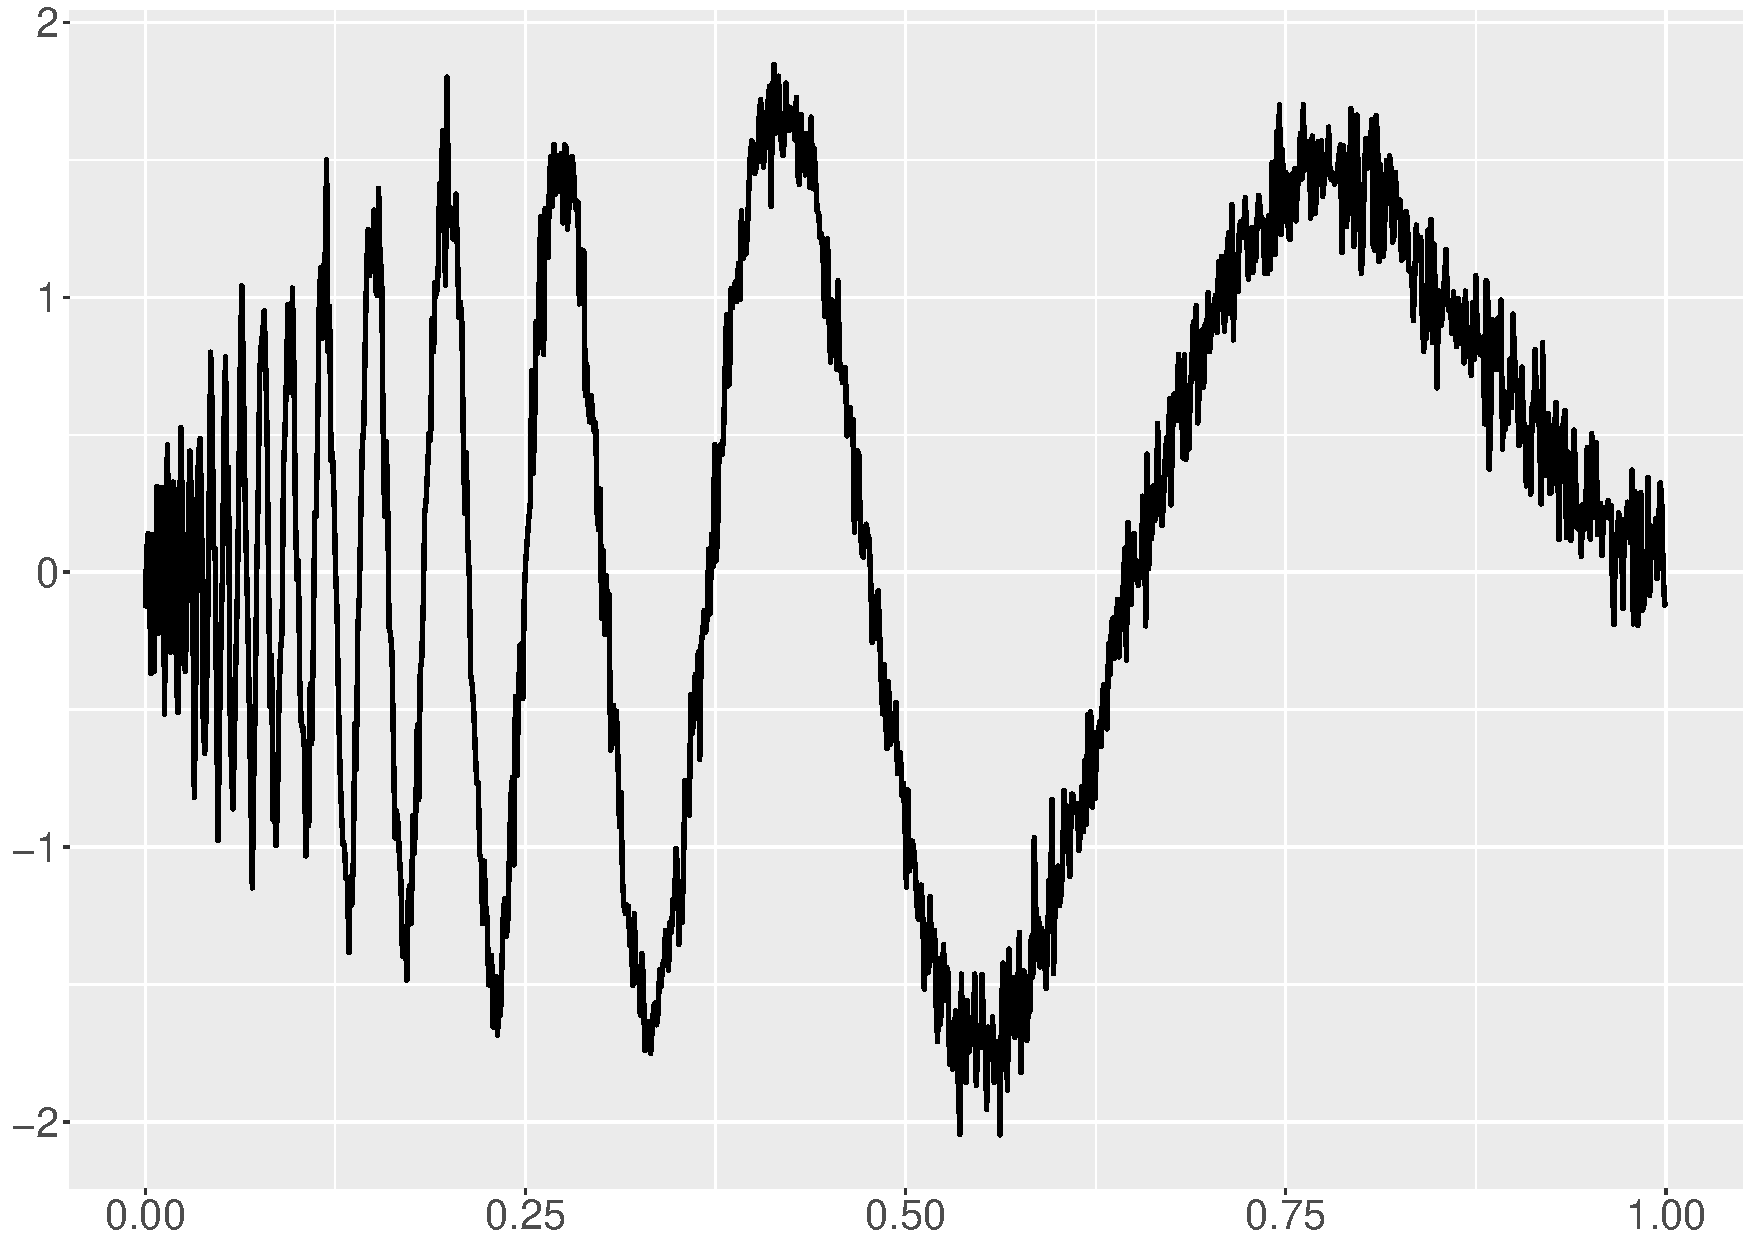
\includegraphics[width=\linewidth,,height=0.45\textwidth]{Chapters/02TractorSplineTheory/plot/ggplot/ggDopplerNoise.pdf}
    \caption{Noisy \textit{Doppler} at \textit{SNR}=7}
    \end{subfigure}
    \begin{subfigure}{0.45\textwidth}
    \centering
    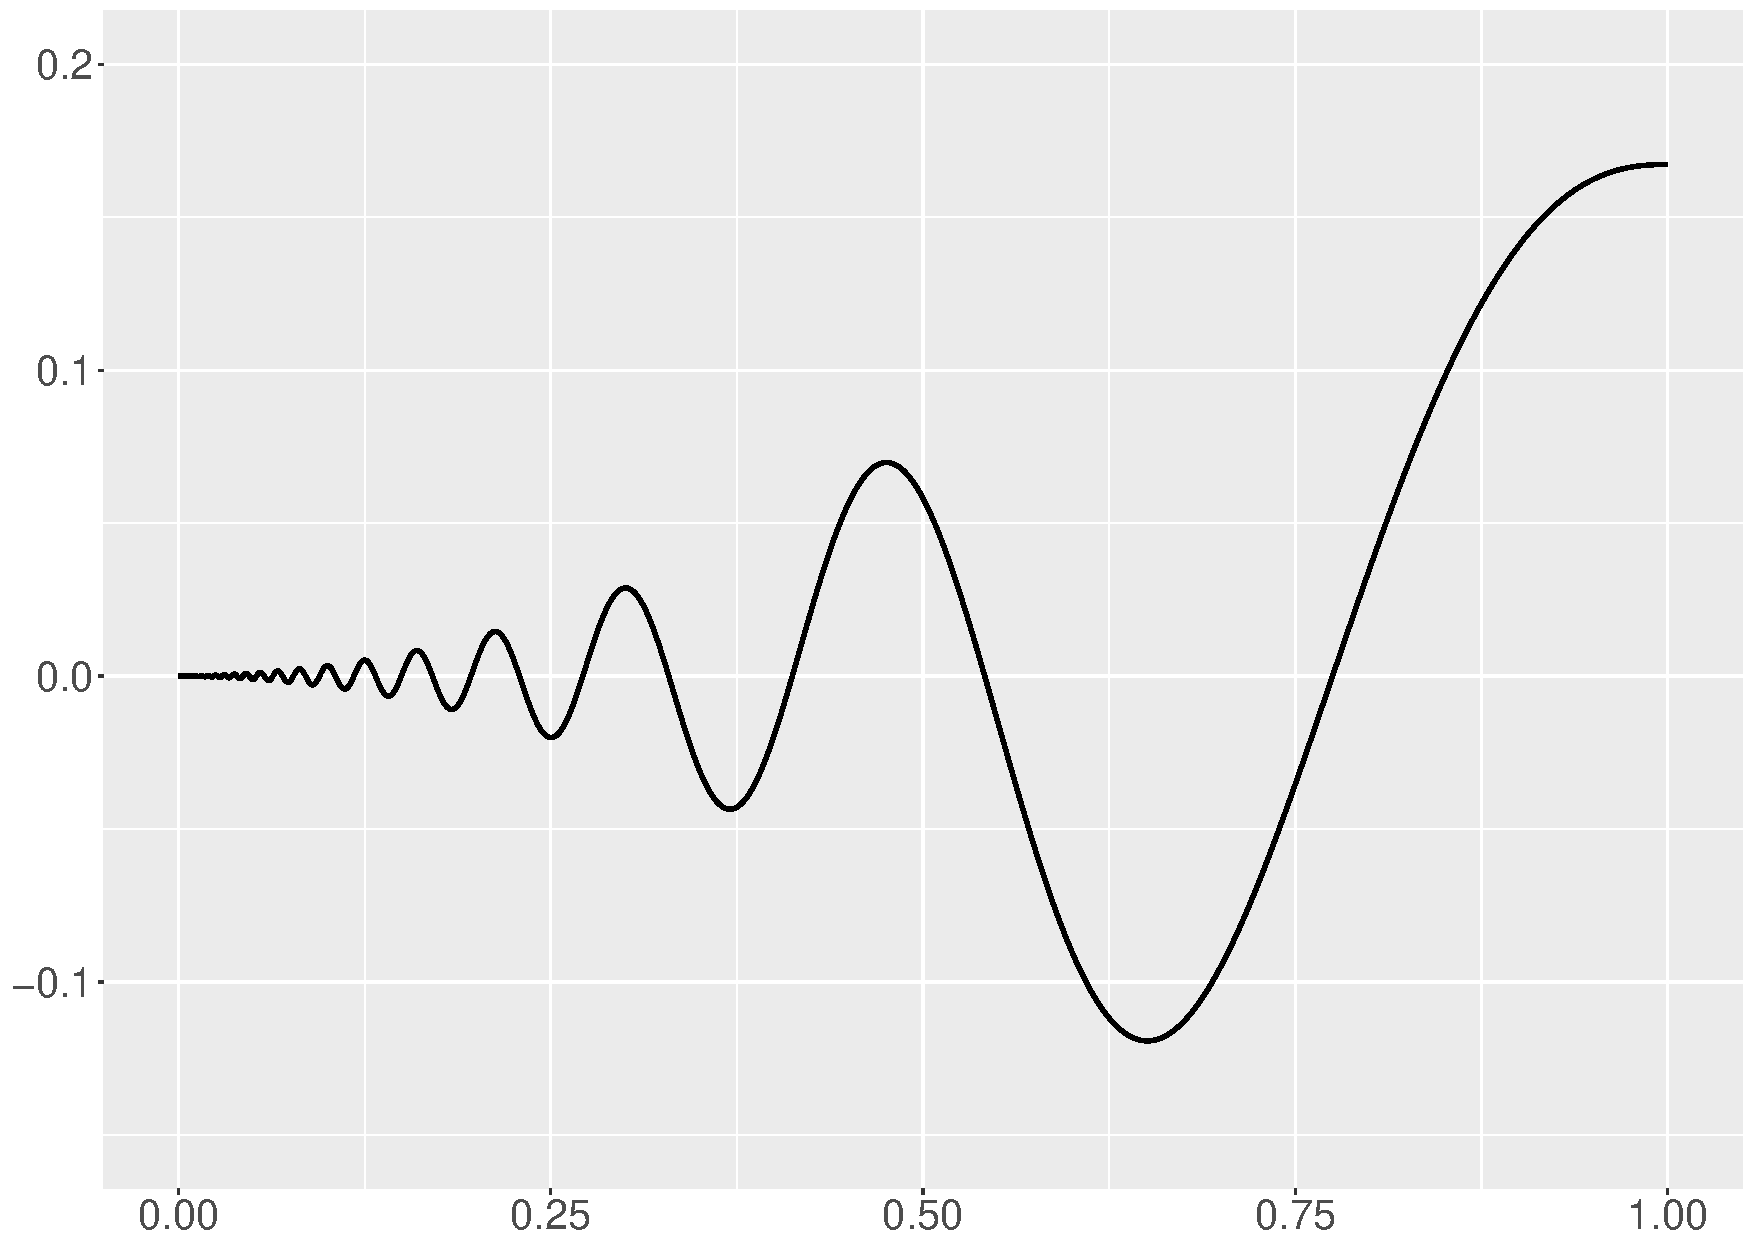
\includegraphics[width=\linewidth,height=0.45\textwidth]{Chapters/02TractorSplineTheory/plot/ggplot/ggDopplerPosition.pdf}
    \caption{Generated positions}
    \end{subfigure}
    \begin{subfigure}{0.45\textwidth}
    \centering
    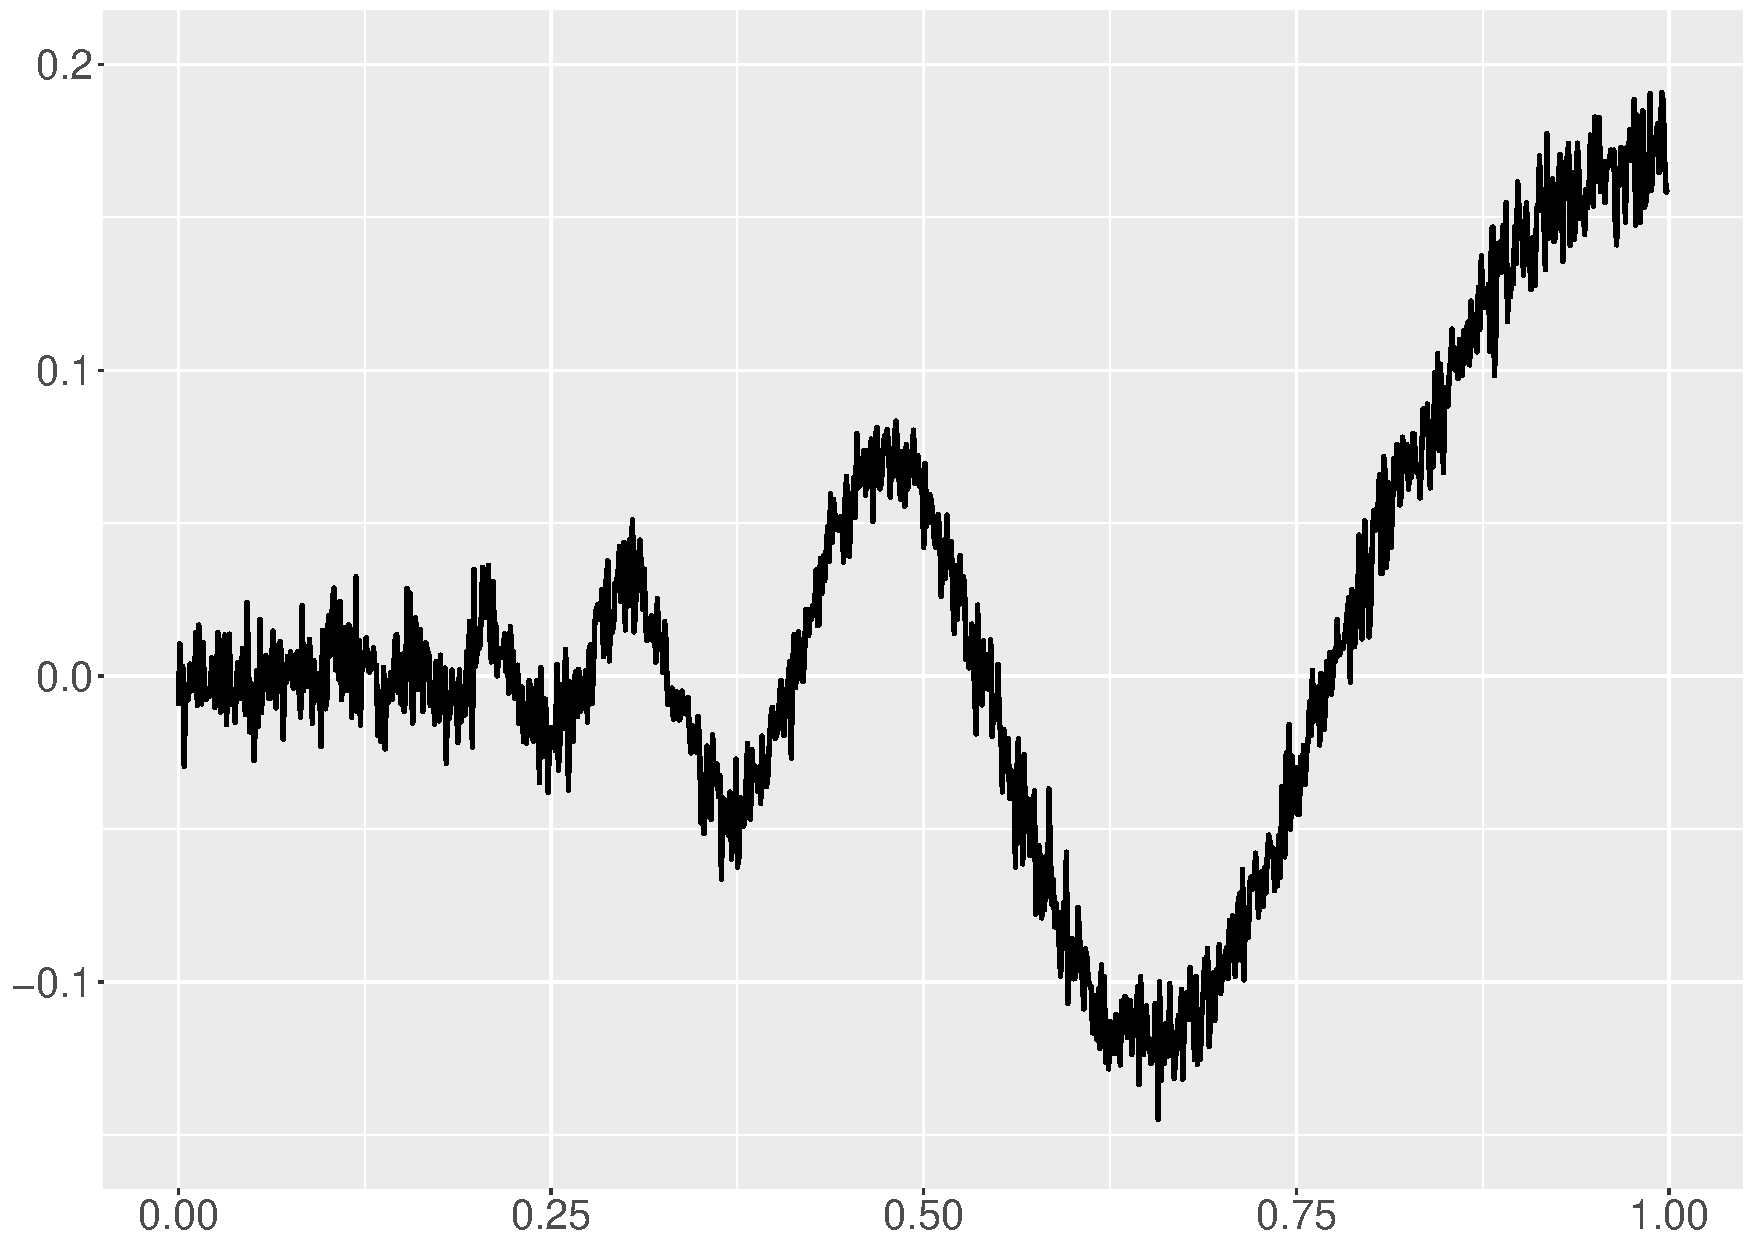
\includegraphics[width=\linewidth,height=0.45\textwidth]{Chapters/02TractorSplineTheory/plot/ggplot/ggDopplerPositionNoise.pdf}
    \caption{Noisy position at \textit{SNR}=7}
    \end{subfigure}
    \begin{subfigure}{0.45\textwidth}
    \centering
    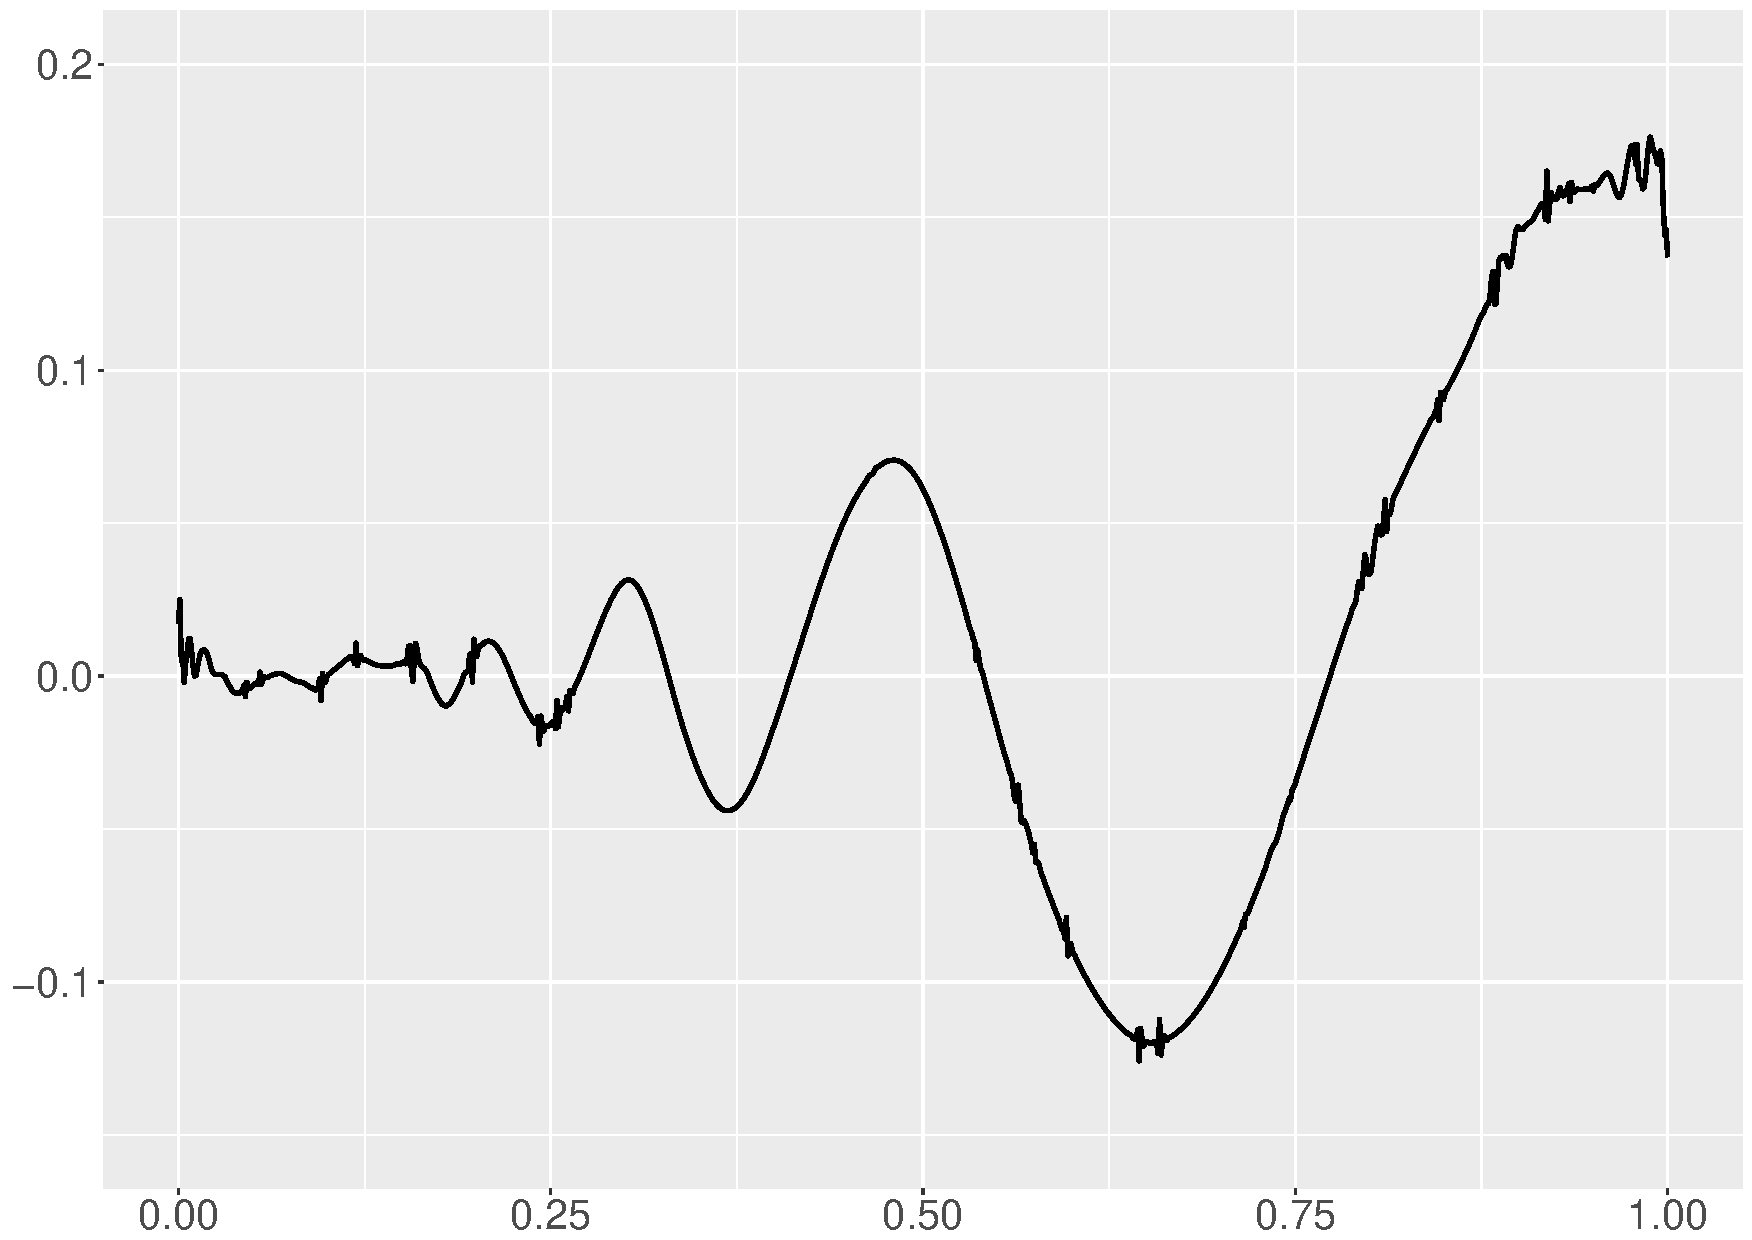
\includegraphics[width=\linewidth,height=0.45\textwidth]{Chapters/02TractorSplineTheory/plot/ggplot/ggDopplerSure.pdf}
    \caption{Reconstruction from Wavelet by sure threshold}
    \end{subfigure}
    \begin{subfigure}{0.45\textwidth}
    \centering
    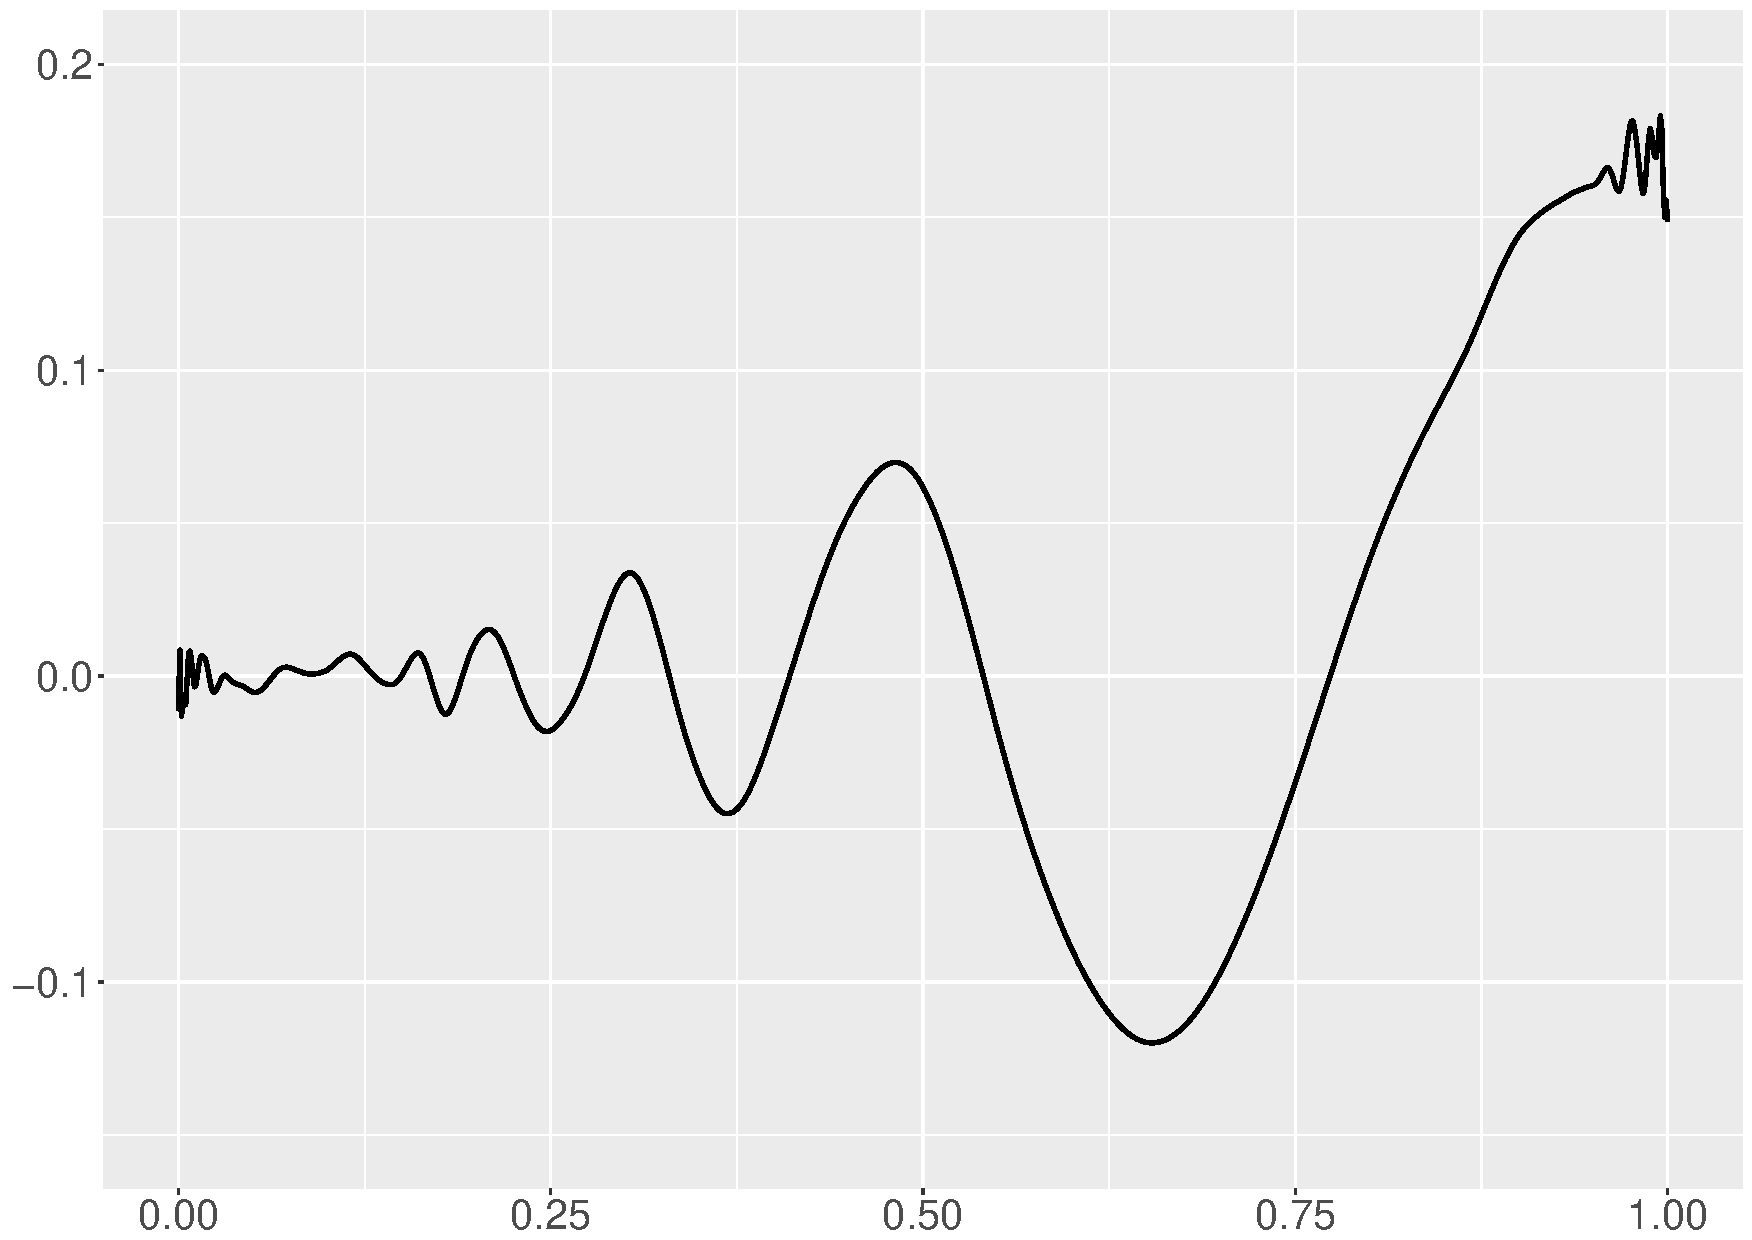
\includegraphics[width=\linewidth,height=0.45\textwidth]{Chapters/02TractorSplineTheory/plot/ggplot/ggDopplerBayes.pdf}
    \caption{Reconstruction from Wavelet by BayesThresh approach}
    \end{subfigure}
    \begin{subfigure}{0.45\textwidth}
    \centering
    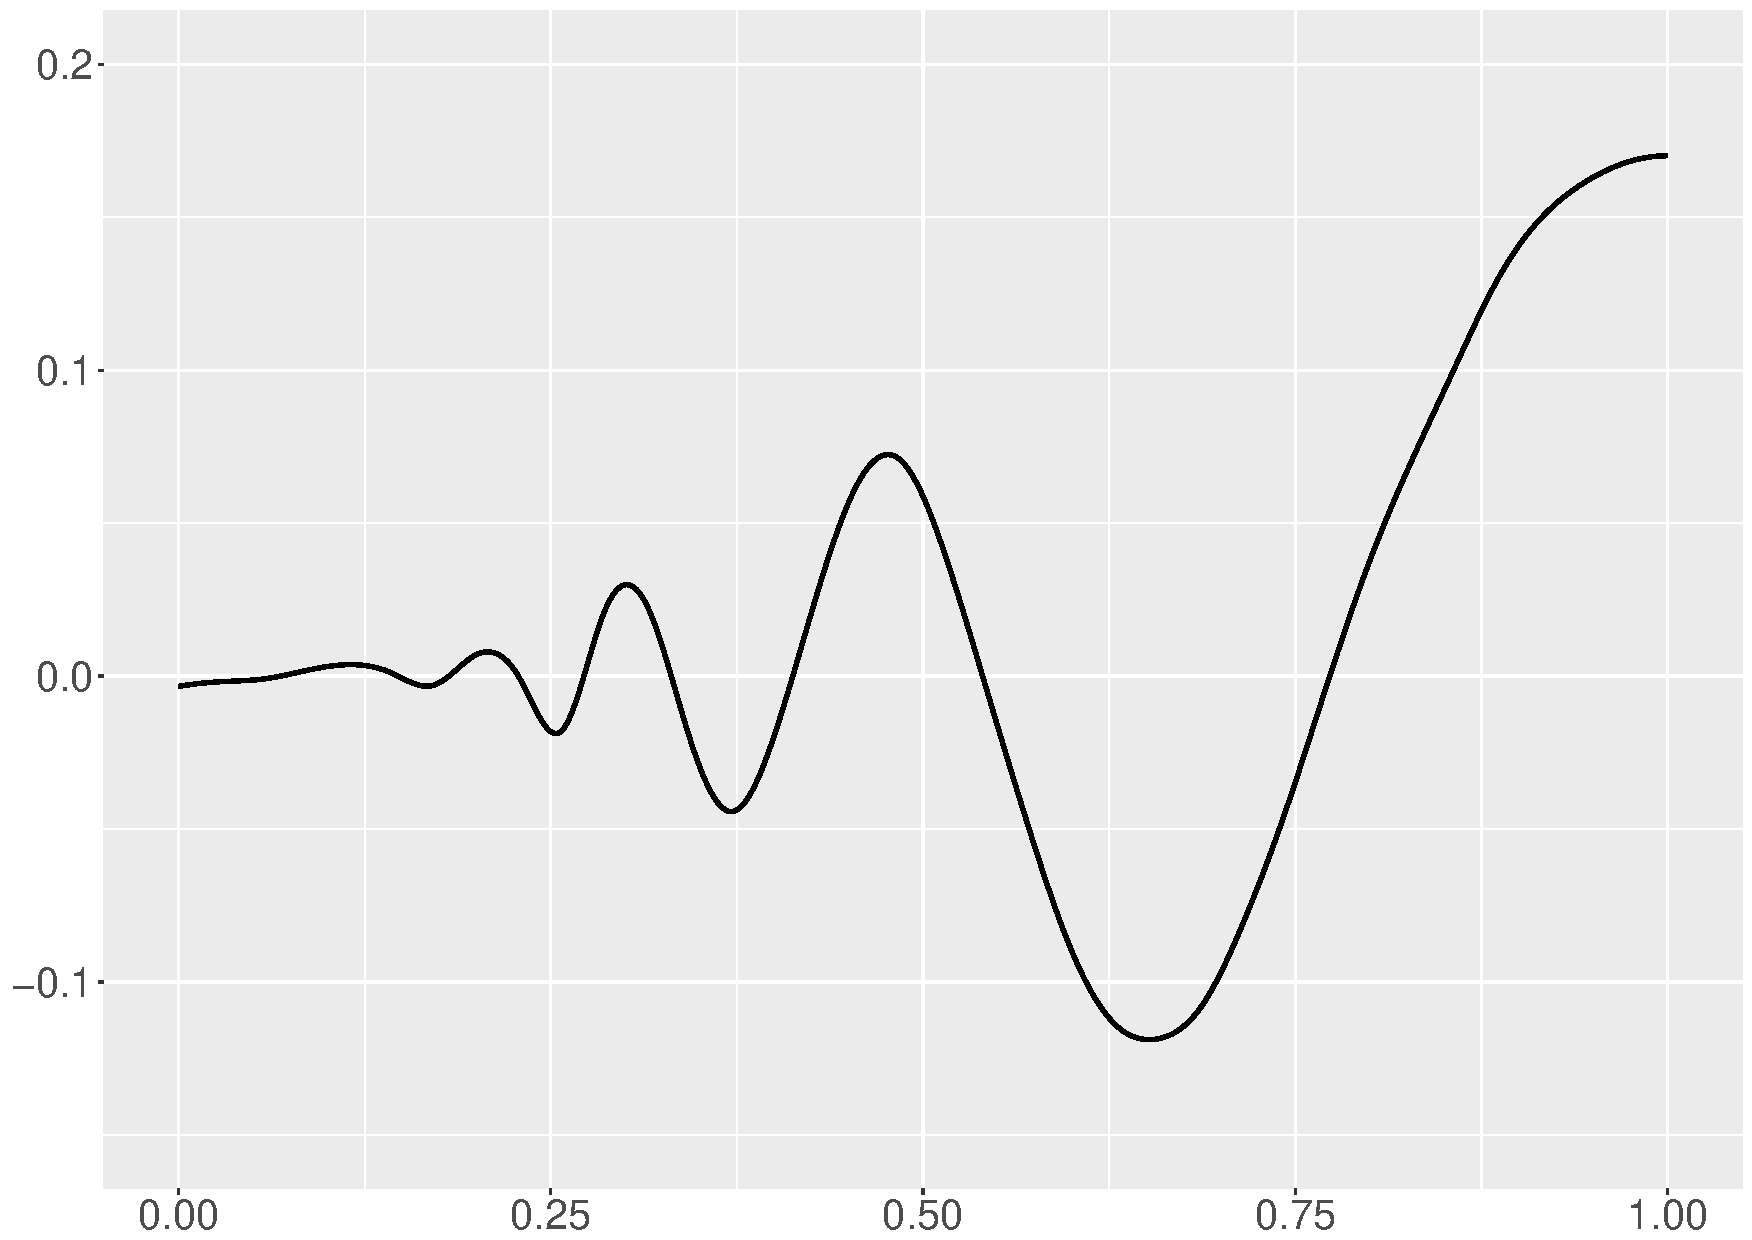
\includegraphics[width=\linewidth,height=0.45\textwidth]{Chapters/02TractorSplineTheory/plot/ggplot/ggDopplerPSpline.pdf}
    \caption{Reconstruction by P-spline \\\mbox{  } }
    \end{subfigure}
    \begin{subfigure}{0.45\textwidth}
    \centering
    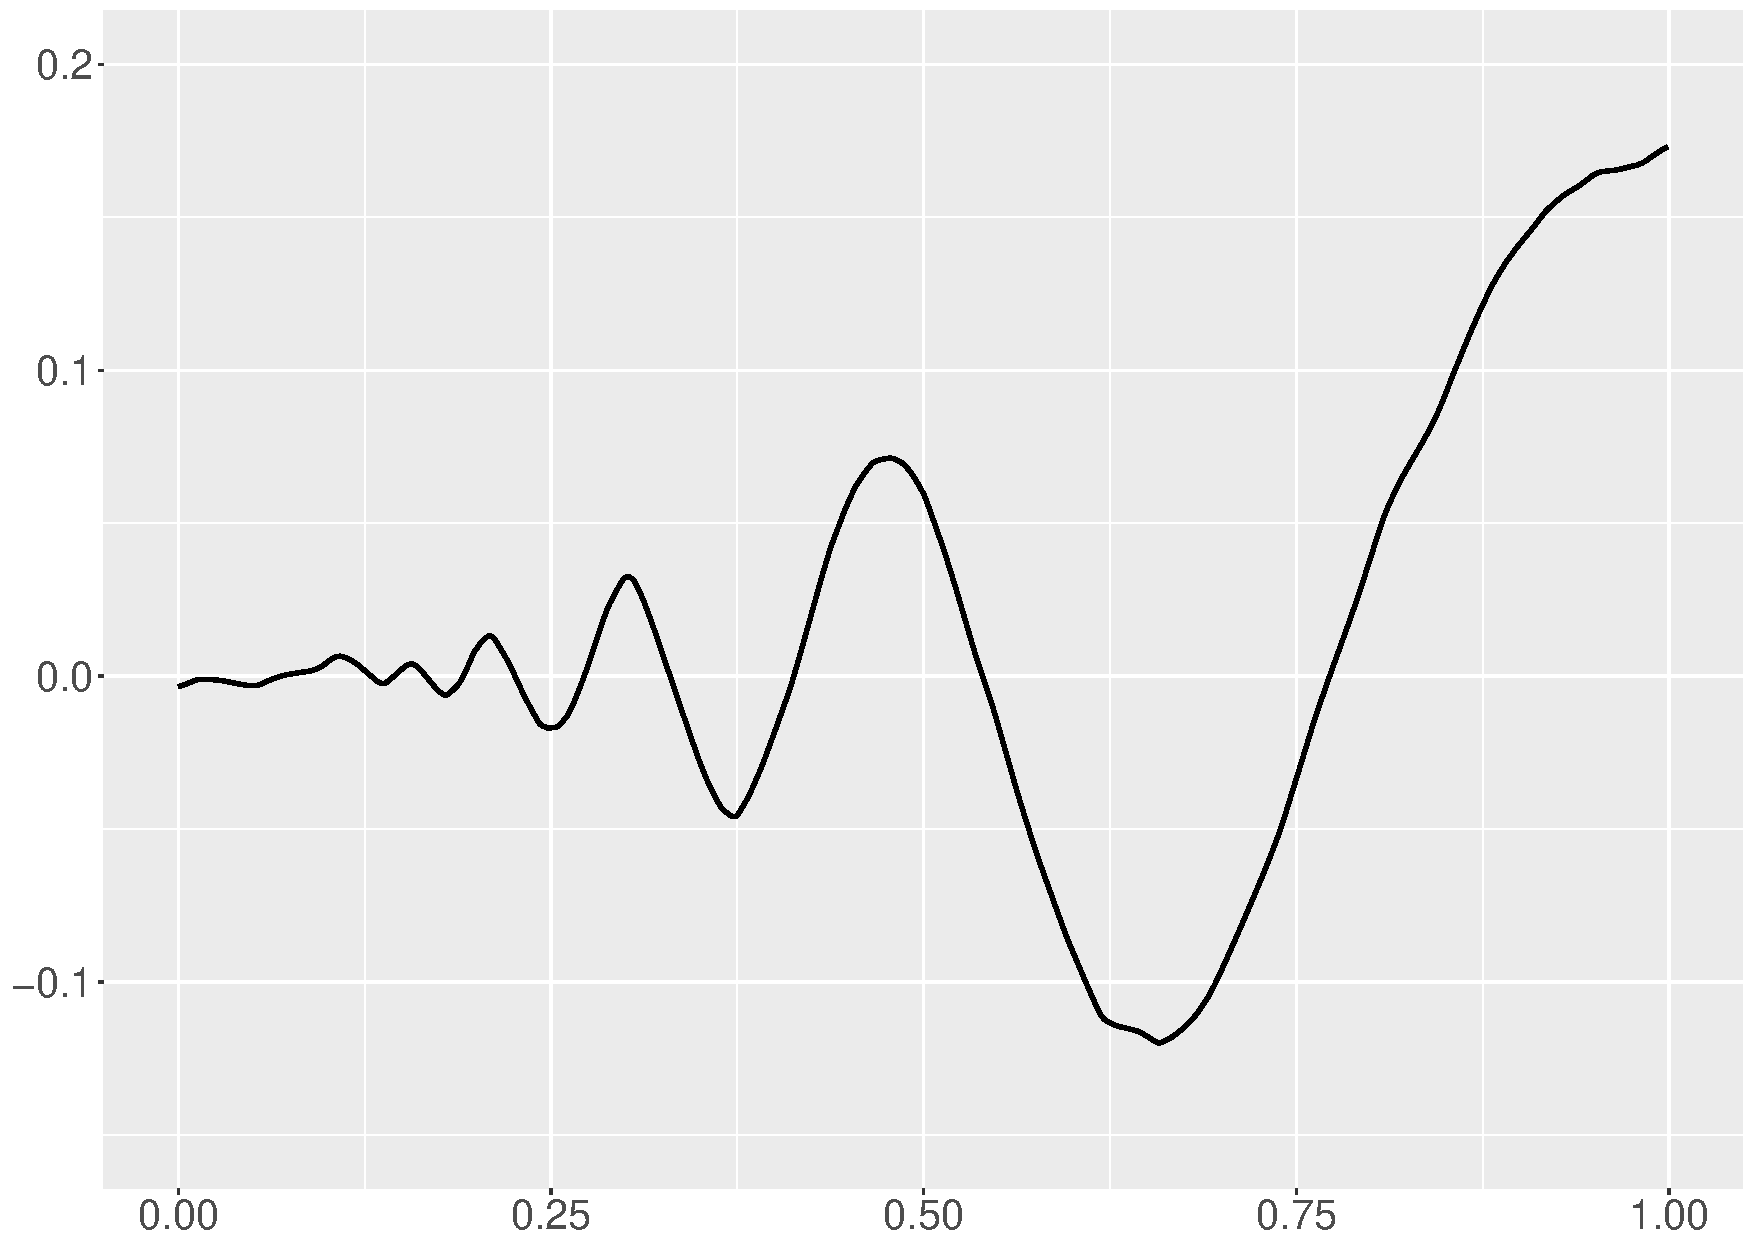
\includegraphics[width=\linewidth,height=0.45\textwidth]{Chapters/02TractorSplineTheory/plot/ggplot/ggDopplerGamma.pdf}
    \caption{Reconstruction by V-spline setting $\gamma=0$}
    \end{subfigure}
  \begin{subfigure}{0.45\textwidth}
    \centering
    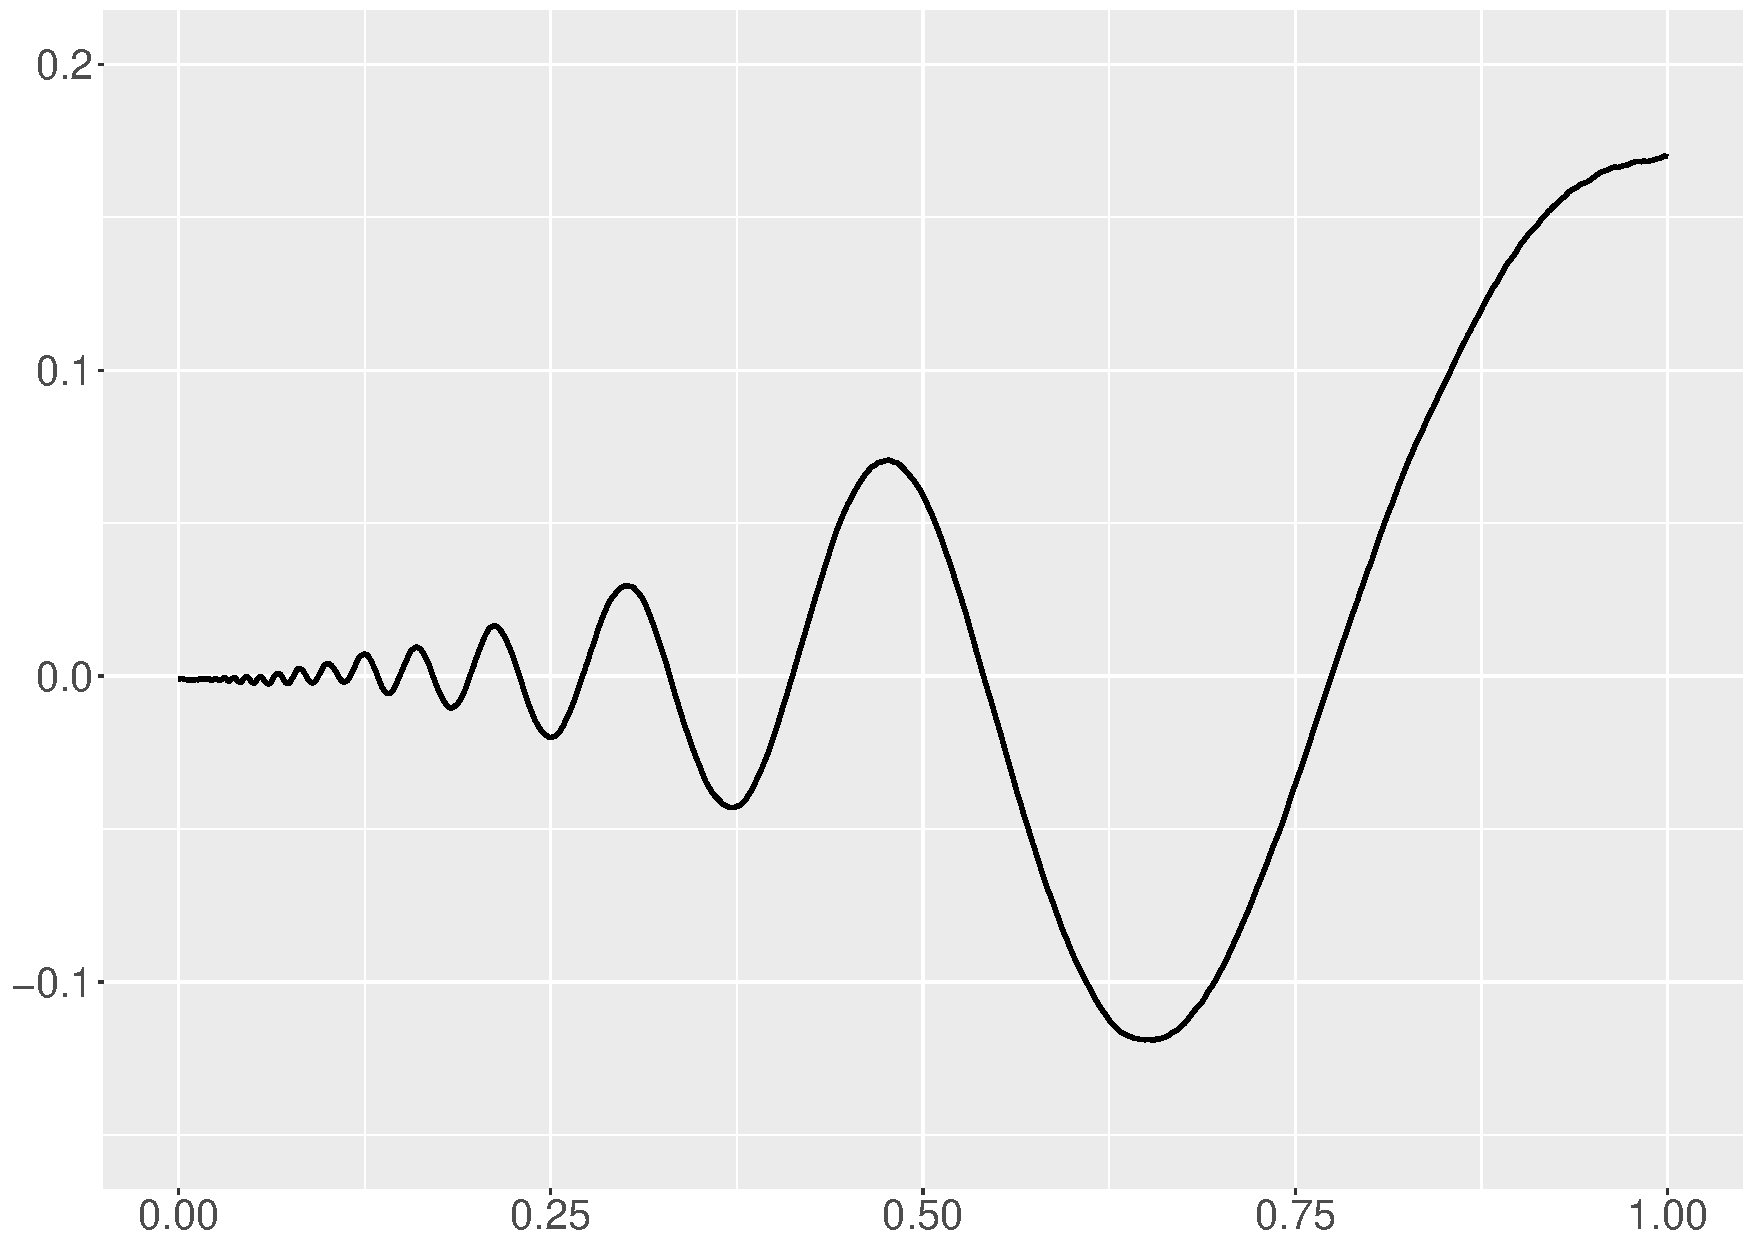
\includegraphics[width=\linewidth,height=0.45\textwidth]{Chapters/02TractorSplineTheory/plot/ggplot/ggDopplerTractorAPT.pdf}
    \caption{Reconstruction by V-spline with conventional penalty term}
    \end{subfigure}
    \begin{subfigure}{0.45\textwidth}
    \centering
    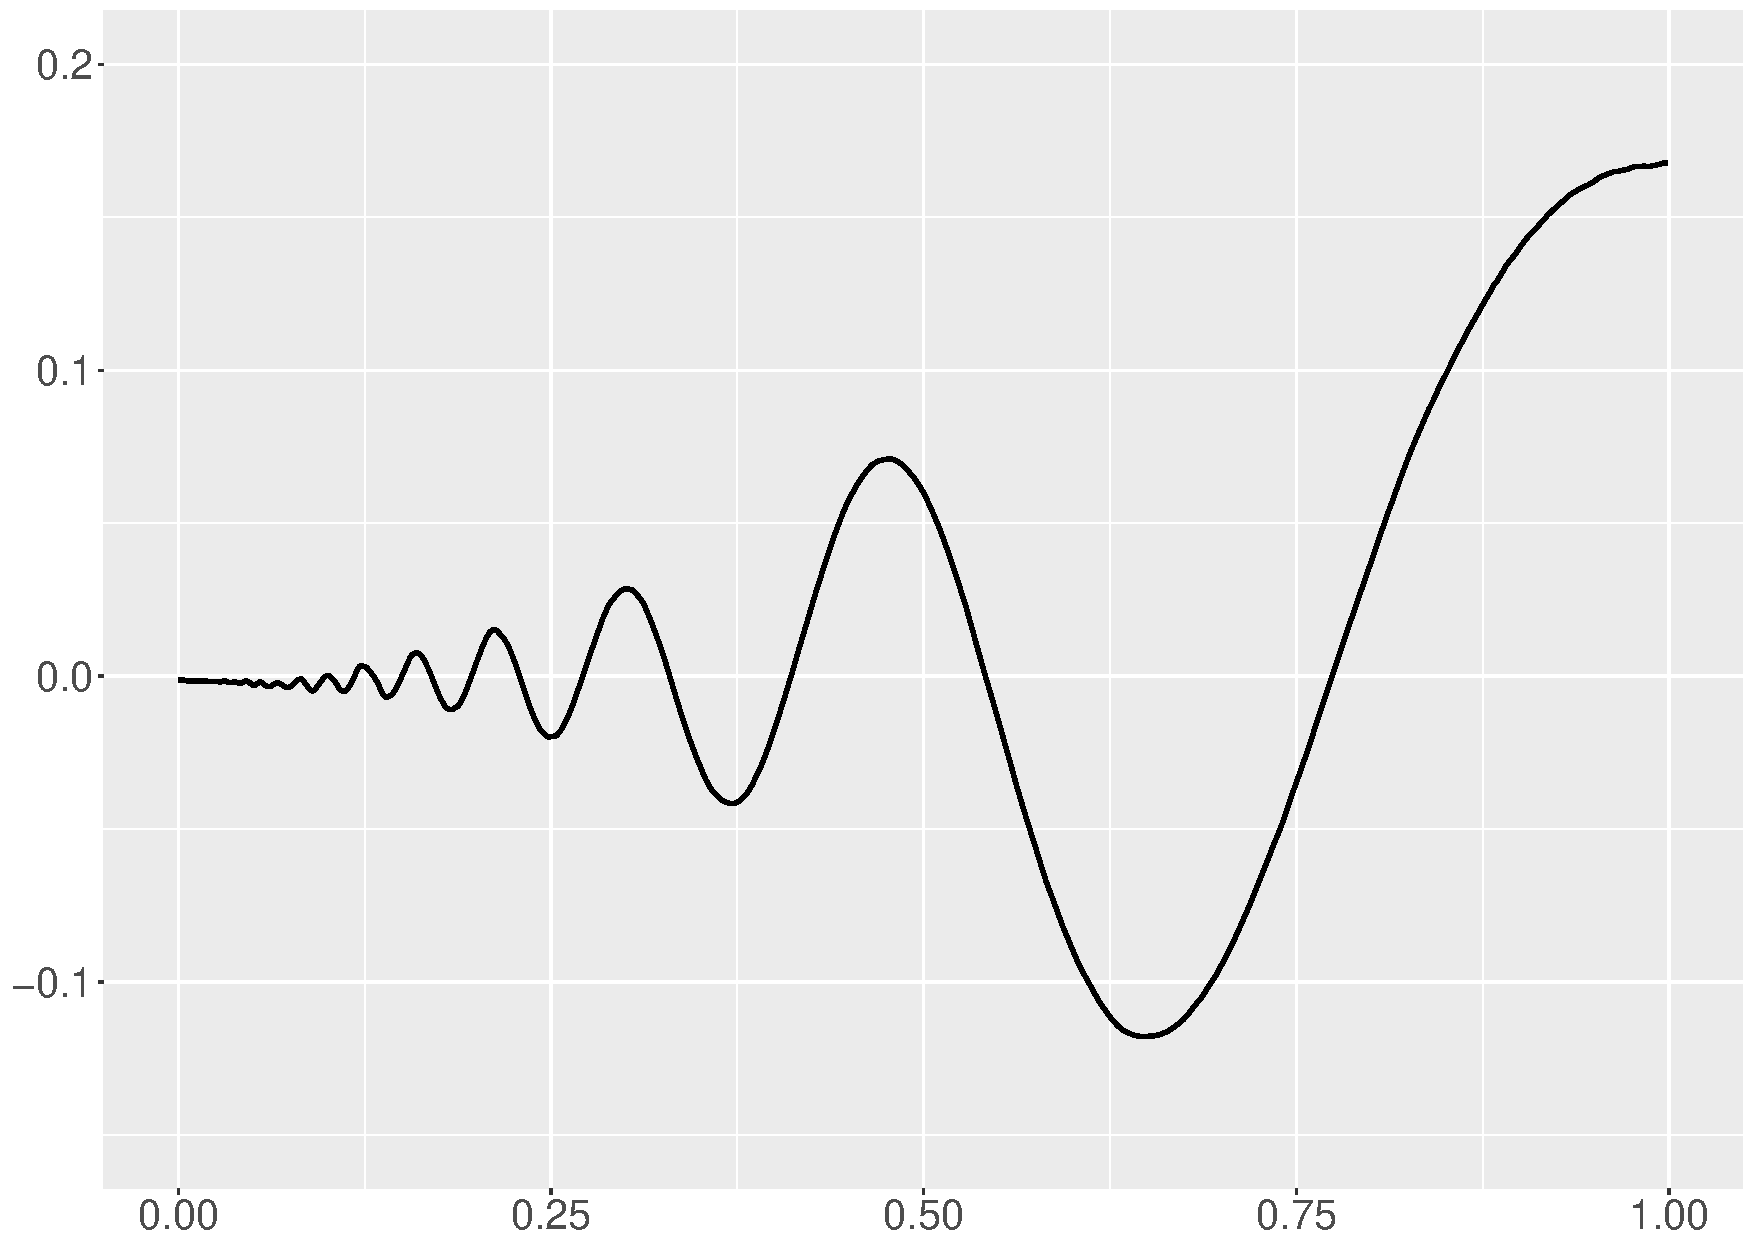
\includegraphics[width=\linewidth,height=0.45\textwidth]{Chapters/02TractorSplineTheory/plot/ggplot/ggDopplerTractor.pdf}
    \caption{Reconstruction by the proposed V-spline.}
    \end{subfigure}
\caption{Numerical example: $\textit{Doppler}$. Comparison of different reconstruction methods with simulated data}\label{num4}
 \end{figure}

By comparing, we can see that all these methods can rebuild up the skeleton of generated trajectory. \textit{Wavelet(sure)} method has more wiggles in interior interval than \textit{Wavelet(BayesThresh)} does, and the latter one becomes fluctuation near boundary knots. \textit{P-spline} gives a smoother fitting than wavelets, but the drawback is lack of specific details. V-spline without velocity loses some information, as can be seen from \textit{Blocks} and \textit{Bumps} where there should be a straight line. V-spline without adjusted penalty term gets over-fitting when the direction changes more frequently than normal, although it catches specific feature in \textit{HeaviSine}. The proposed V-spline performs much better than other methods and returns the near-true trajectory reconstructions.  



%and is larger when the function trying to change directions. We only have a couple of large penalty terms in $\textit{Blocks}$ and $\textit{Bumps}$ function, as most of the time they were moving in straight line. More curves are in $\textit{HeaviSine}$ and $\textit{Doppler}$ functions, so the penalty term try to catch more information and ignore noises. 
%\begin{figure}
%  \centering
%         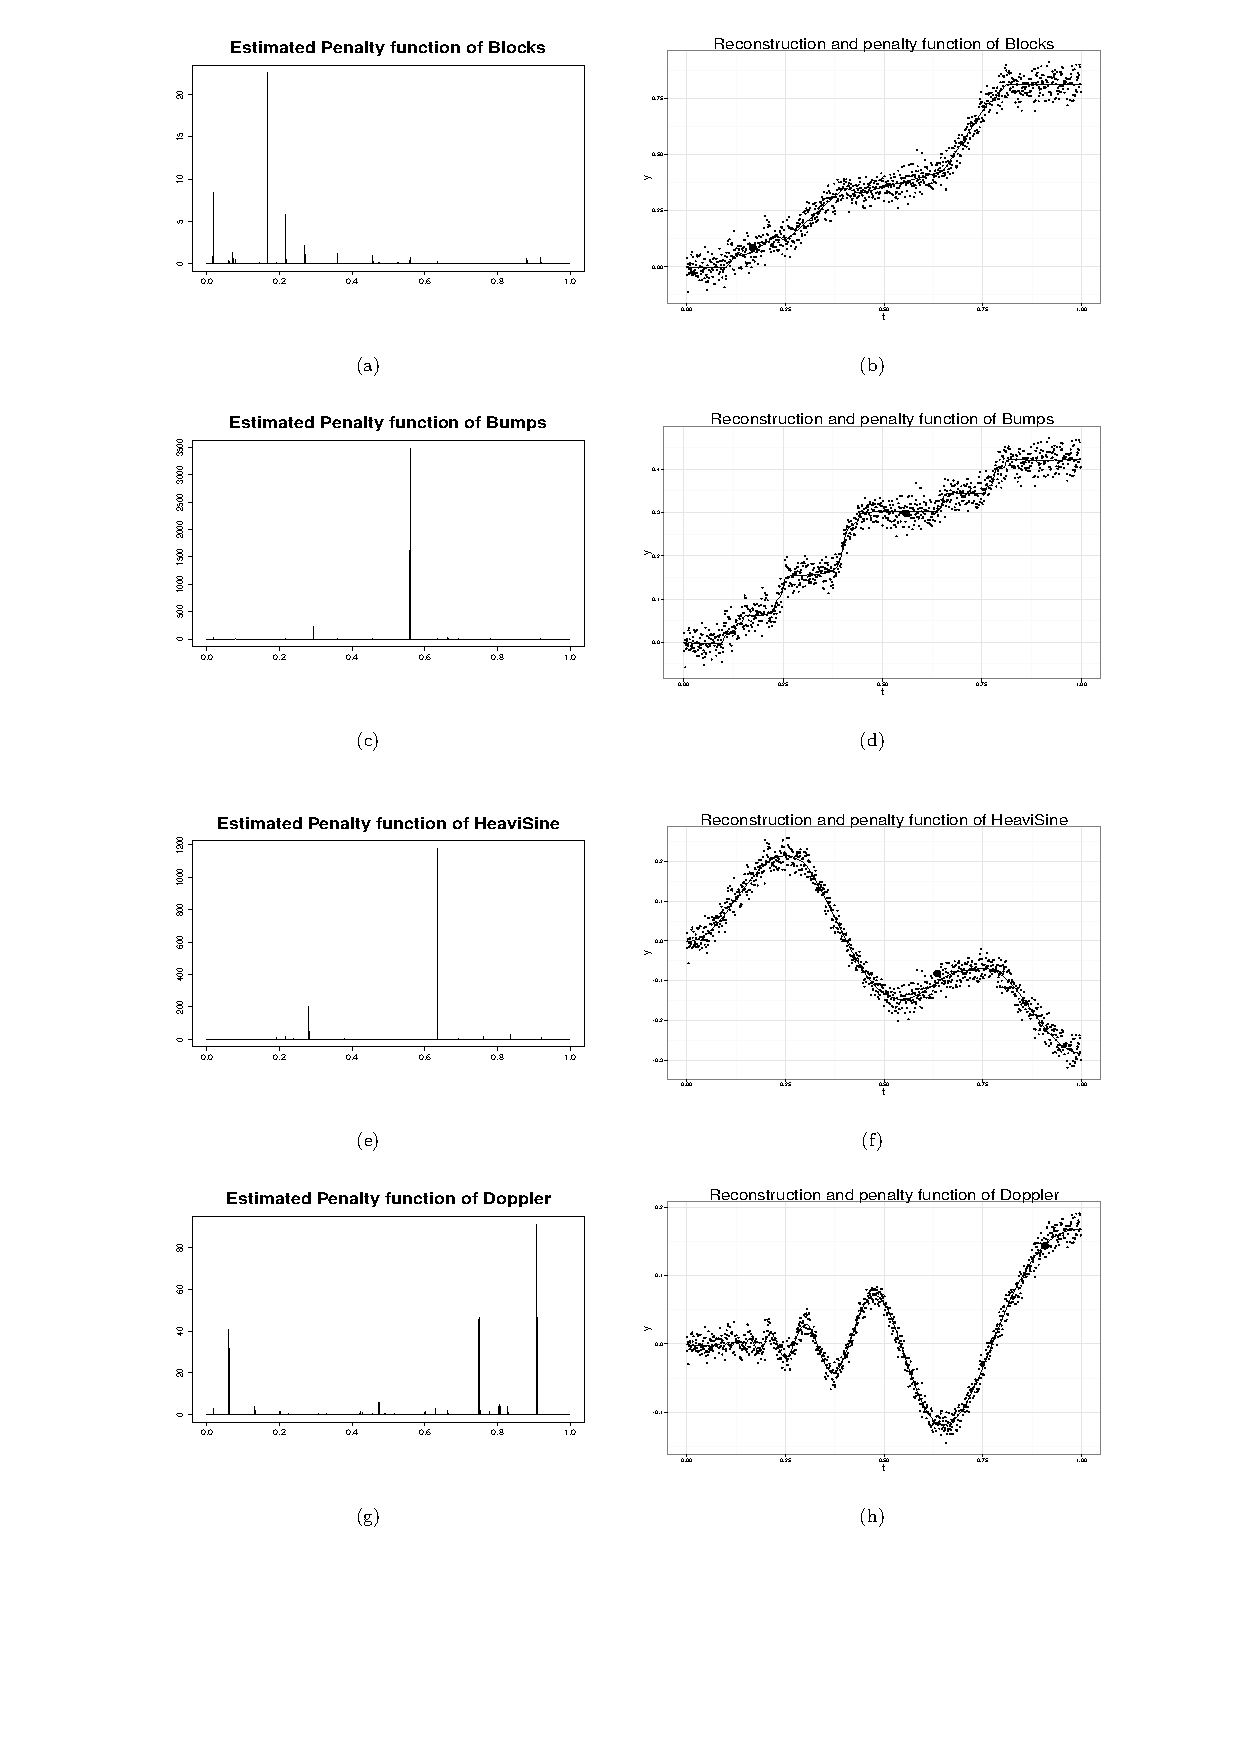
\includegraphics[width=\textwidth,height=14cm]{Chapters/02TractorSplineTheory/plot/penalty08} 
%  \caption{Estimated penalty functions. Left side shows how the value of $\lambda(t)$ changes on the interval. Right side projects $\lambda(t)$ into reconstructions. The bigger the blacks dots present, the larger the penalty values are.}\label{numpenalty}
%\end{figure}

\begin{figure}
    \centering
    \begin{subfigure}{\textwidth}
    \centering
    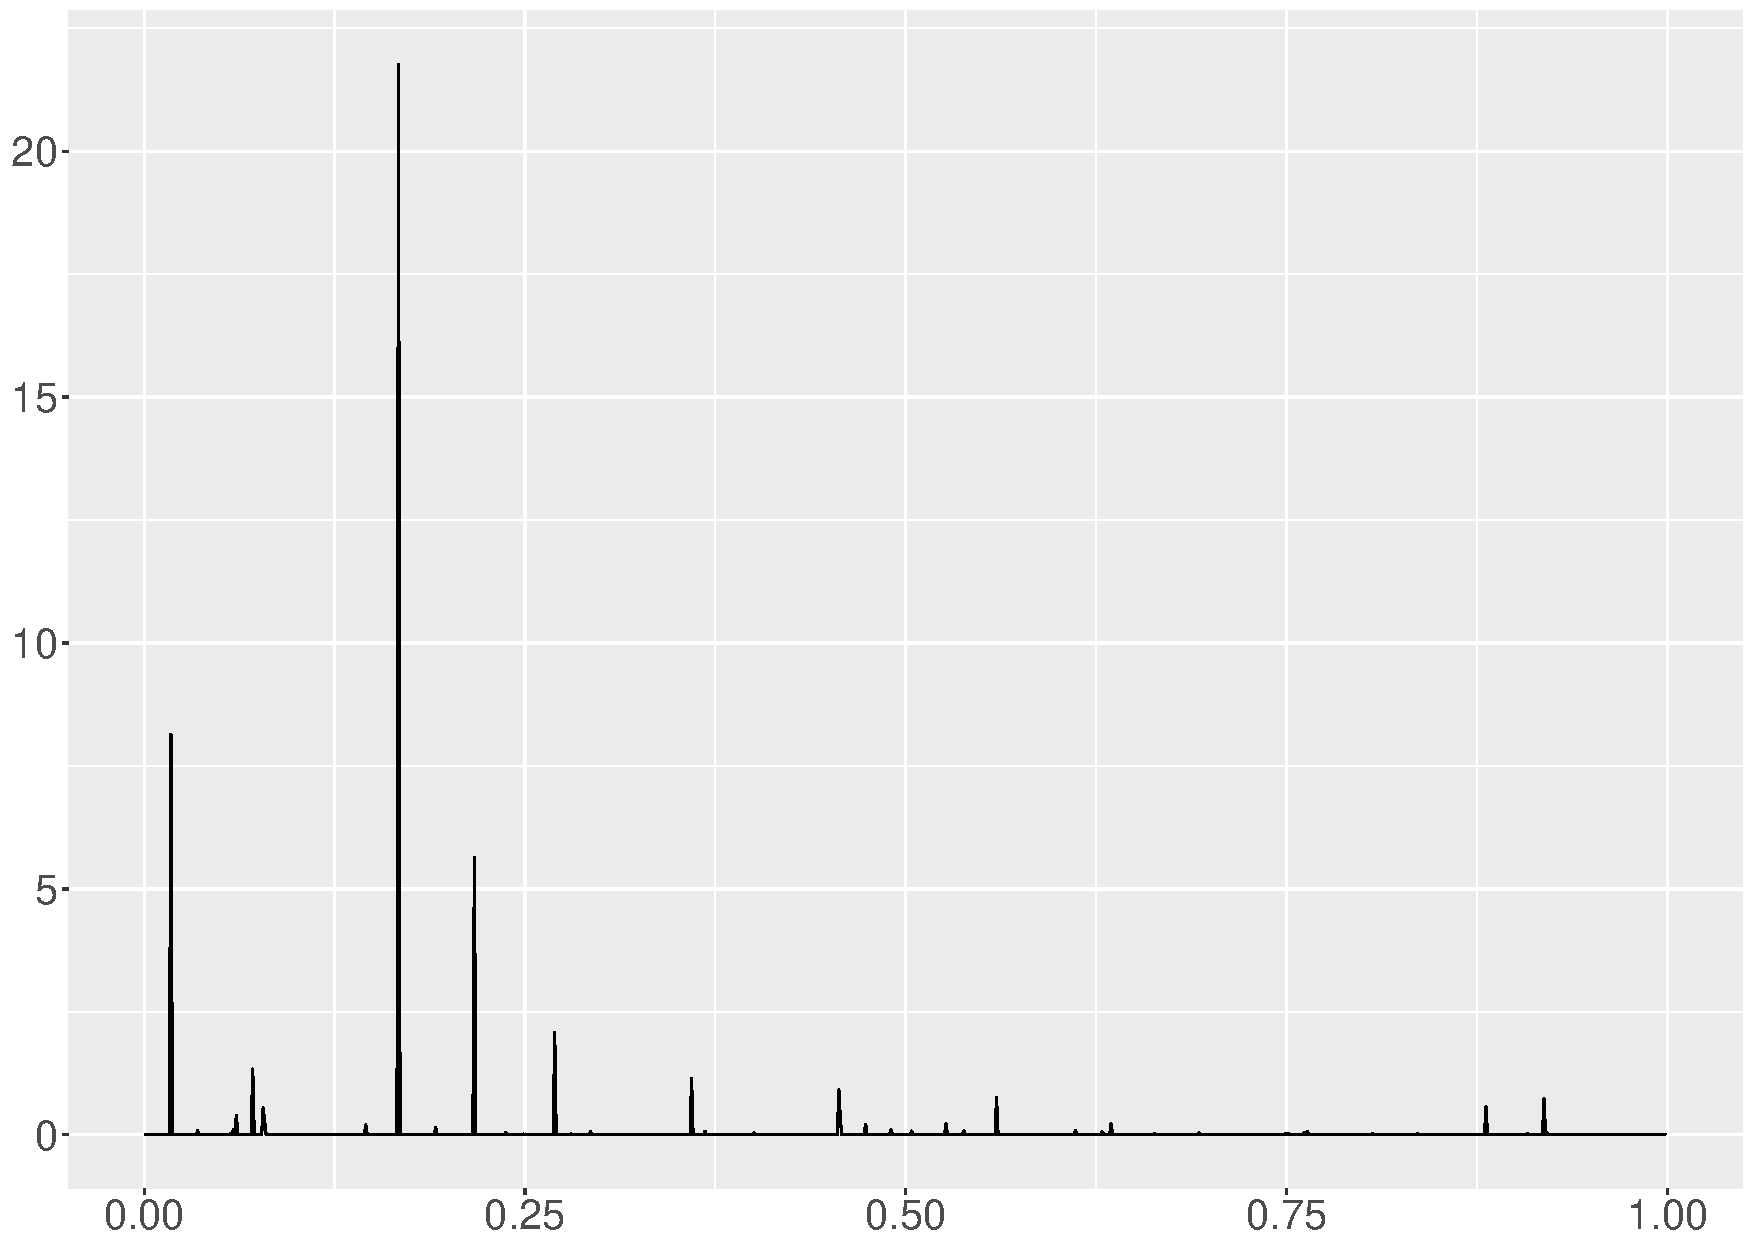
\includegraphics[width=0.45\textwidth]{Chapters/02TractorSplineTheory/plot/ggplot/ggBlocksPenaltyBar.pdf}
    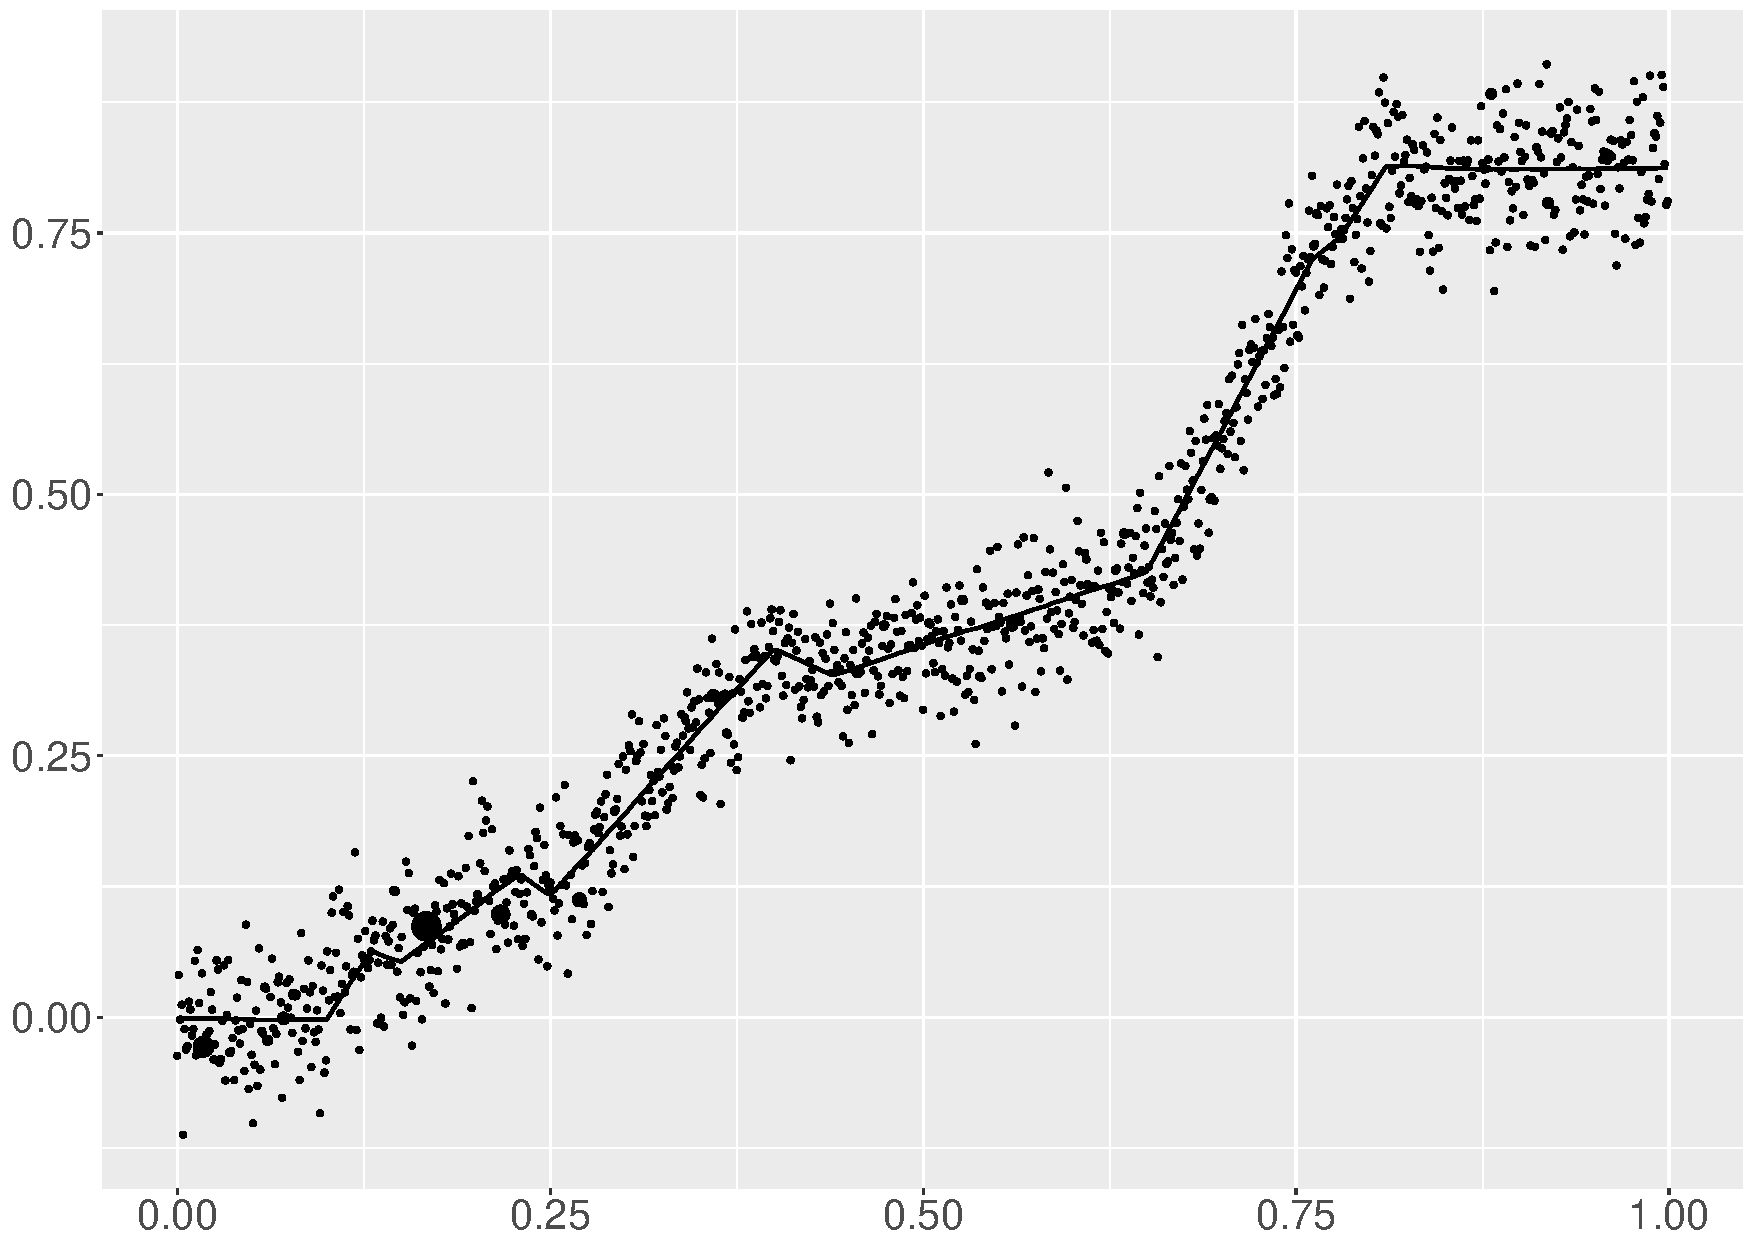
\includegraphics[width=0.45\textwidth]{Chapters/02TractorSplineTheory/plot/ggplot/ggBlocksPenaltyLine.pdf}
    \caption{Distribution of the penalty values in reconstructed \textit{Blocks}}
    \end{subfigure}
    \begin{subfigure}{\textwidth}
    \centering
    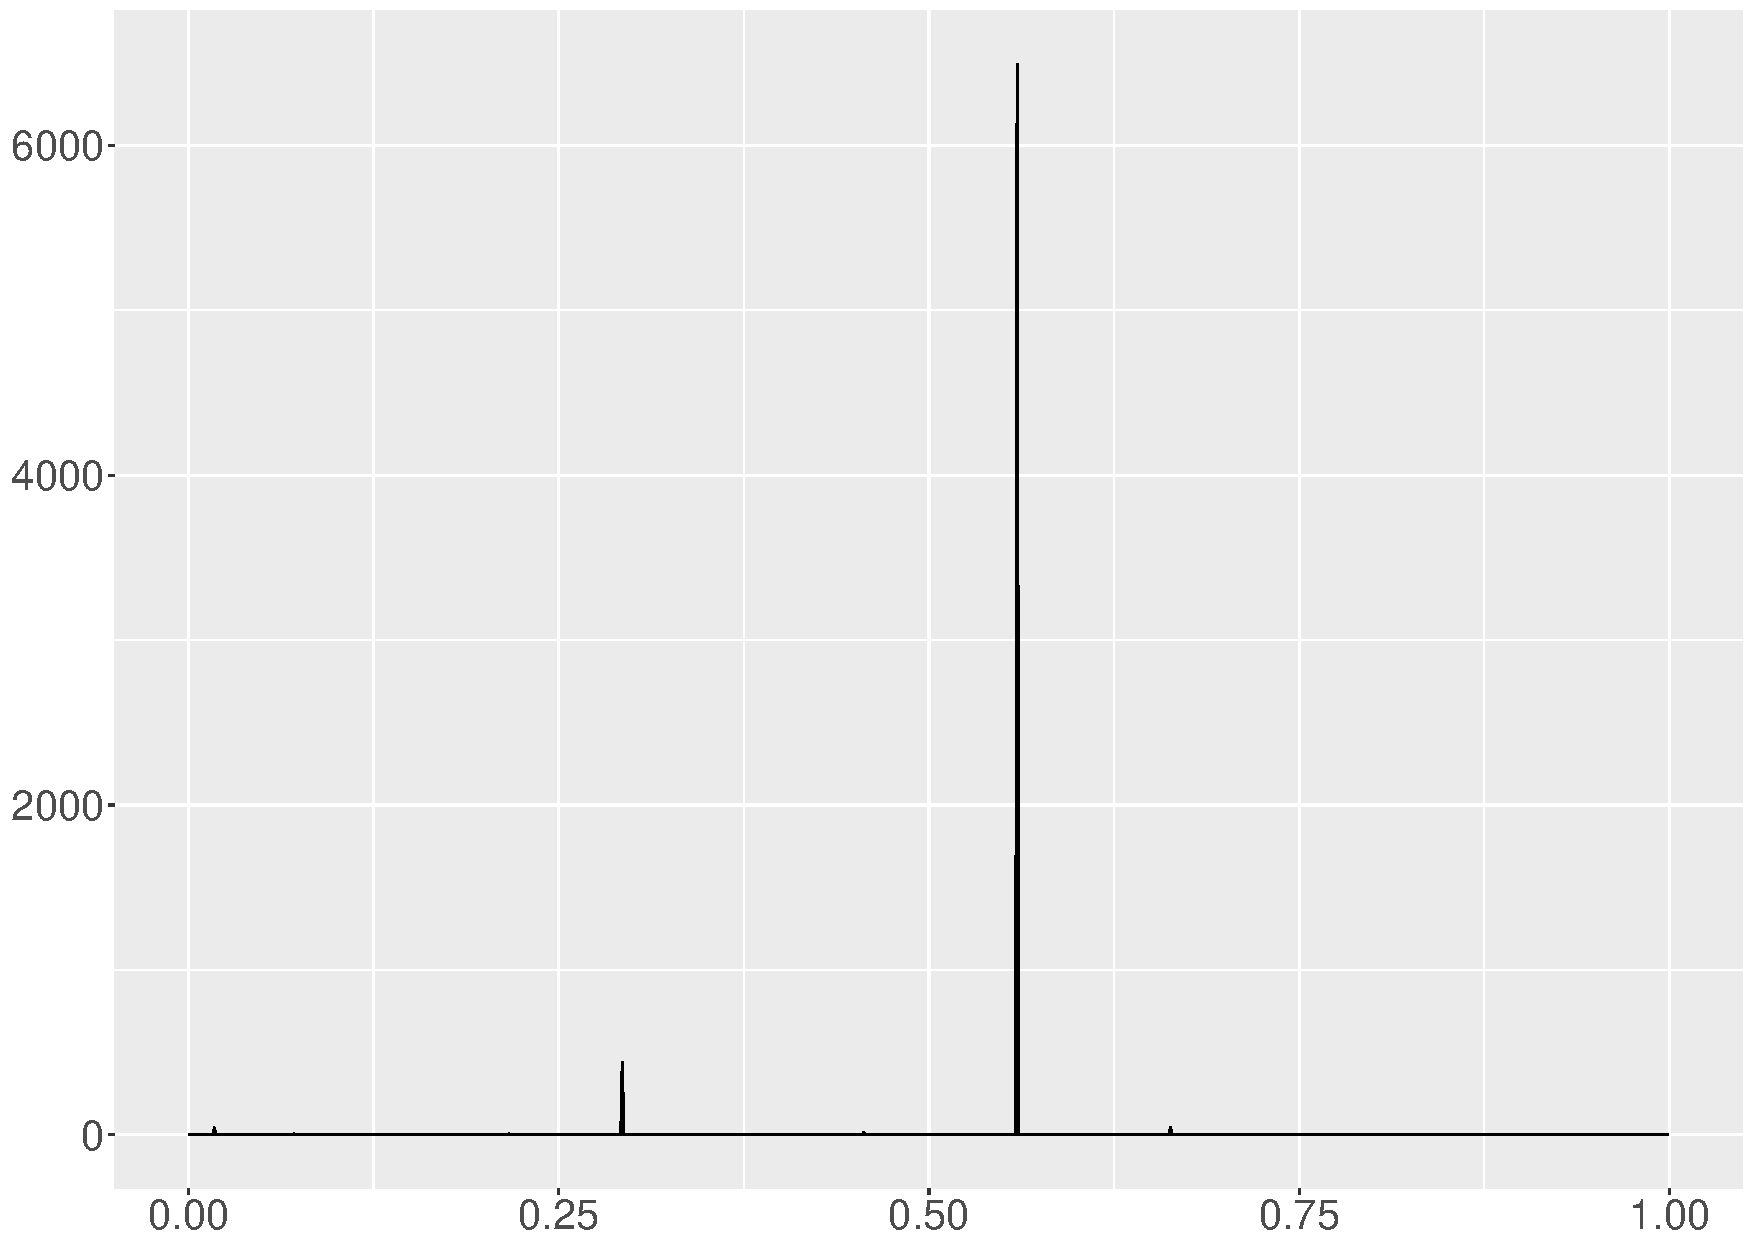
\includegraphics[width=0.45\textwidth]{Chapters/02TractorSplineTheory/plot/ggplot/ggBumpsPenaltyBar.pdf}
    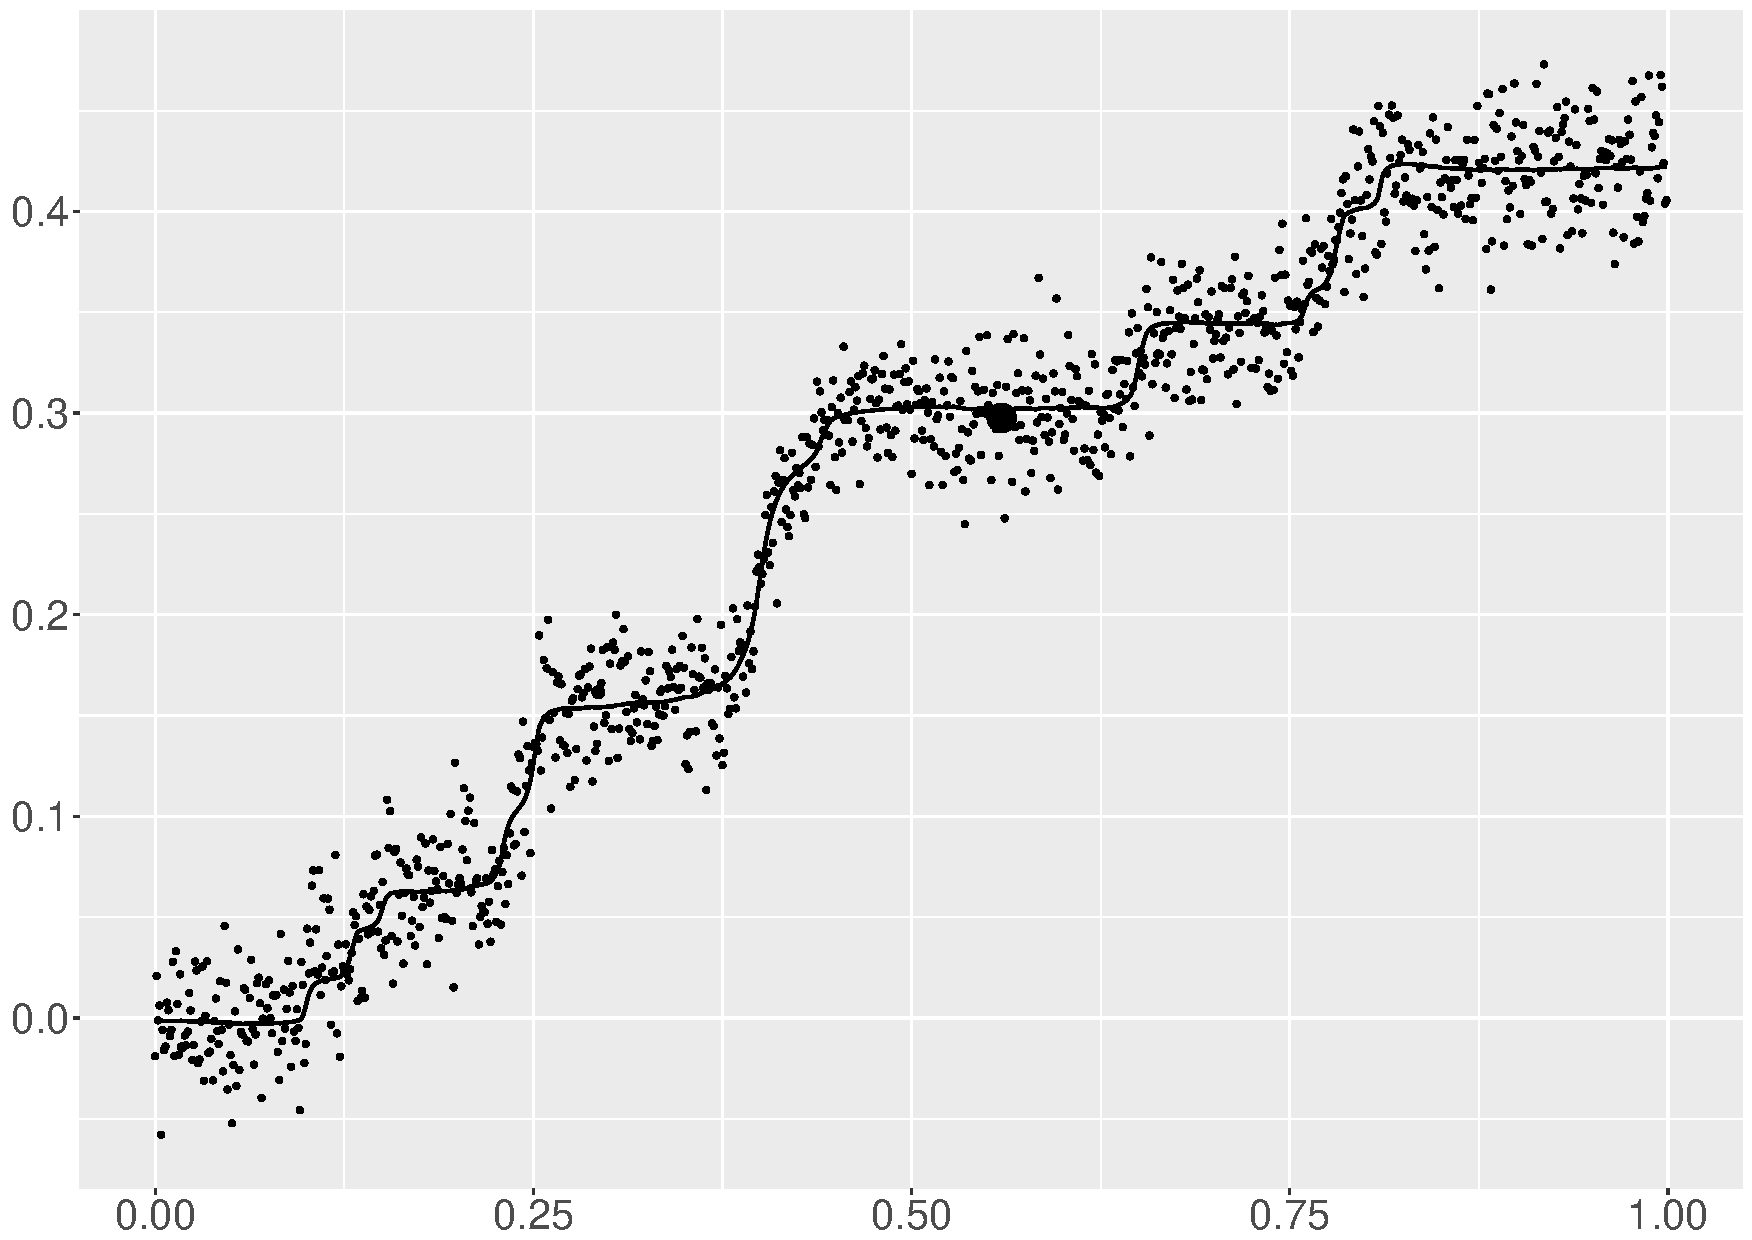
\includegraphics[width=0.45\textwidth]{Chapters/02TractorSplineTheory/plot/ggplot/ggBumpsPenaltyLine.pdf}
    \caption{Distribution of the penalty values in reconstructed \textit{Bumps}}
    \end{subfigure}
    \begin{subfigure}{\textwidth}
    \centering
    \includegraphics[width=0.45\textwidth]{Chapters/02TractorSplineTheory/plot/ggplot/ggHeaviSinePenaltyBar.pdf}
    \includegraphics[width=0.45\textwidth]{Chapters/02TractorSplineTheory/plot/ggplot/ggHeaviSinePenaltyLine.pdf}
    \caption{Distribution of the penalty values in reconstructed \textit{HeaviSine}}
    \end{subfigure}
\end{figure}
\begin{figure}\ContinuedFloat
    \centering 
    \begin{subfigure}{\textwidth}
    \centering
    \includegraphics[width=0.45\textwidth]{Chapters/02TractorSplineTheory/plot/ggplot/ggDopplerPenaltyBar.pdf}
    \includegraphics[width=0.45\textwidth]{Chapters/02TractorSplineTheory/plot/ggplot/ggDopplerPenaltyLine.pdf}
    \caption{Distribution of the penalty values in reconstructed \textit{Doppler}}
    \end{subfigure}
\caption{Distribution of the penalty values $\lambda(t)$ in V-spline. Figures on the left side indicate the values varying in intervals. On the right side, these values are projected into reconstructions. The bigger the blacks dots present, the larger the penalty values are.}\label{numpenalty}
\end{figure}


Figure \ref{numpenalty} shows the estimated penalty values $\lambda(t)=\frac{\left(\Delta t\right)^3}{\left(\Delta d\right)^2}\lambda$ at SNR=7. The figures in the left column illustrate the values of the penalty term at different intervals, the figures in the right column are the observations and reconstructed trajectory. Bigger black dots present larger penalty values. It can be seen that $\lambda(t)$ adapts to the smoothness pattern of position and will be large where a long time gap may occur. The details of how this penalty function works will be explained in next subsection. Figure \ref{TractorsplineSNR3} illustrates the reconstructions of V-spline at SNR=3.


%\begin{figure}
%\centering
%%  \begin{landscape}
%         \includegraphics[width=\textwidth,height=9cm]{Chapters/02TractorSplineTheory/plot/vtractor04} 
%%  \end{landscape}
%     \caption{Estimated velocity functions by taking the first derivative of V-spline. (a) Fitted $\textit{Blocks}$. (b) Fitted $\textit{Bumps}$. (c) Fitted $\textit{HeaviSine}$. (d) Fitted $\textit{Doppler}$.}\label{numvtractor}
%\end{figure}

\begin{figure}
    \centering
    \begin{subfigure}{0.45\textwidth}
    \centering
    \includegraphics[width=\textwidth]{Chapters/02TractorSplineTheory/plot/ggplot/ggBlocksTractorVelocity.pdf}
    \caption{Estimated \textit{Blocks}  }
    \end{subfigure}%
    \begin{subfigure}{0.45\textwidth}
    \centering
    \includegraphics[width=\textwidth]{Chapters/02TractorSplineTheory/plot/ggplot/ggBumpsTractorVelocity.pdf}
    \caption{Estimated \textit{Bumps}  }
    \end{subfigure}
    \begin{subfigure}{0.45\textwidth}
    \centering
    \includegraphics[width=\textwidth]{Chapters/02TractorSplineTheory/plot/ggplot/ggHeaviSineTractorVelocity.pdf}
    \caption{Estimated \textit{HeaviSine}  }
    \end{subfigure}
    \begin{subfigure}{0.45\textwidth}
    \centering
    \includegraphics[width=\textwidth]{Chapters/02TractorSplineTheory/plot/ggplot/ggDopplerTractorVelocity.pdf}
    \caption{Estimated \textit{Doppler}  }
    \end{subfigure}
\caption{Estimated velocity functions by V-spline. The velocity is generated from the original simulation functions by equation \eqref{generateVelocity}}\label{numvtractor}
 \end{figure}



Figure \ref{numvtractor} demonstrates the estimated velocity functions. By taking the first derivative of fitted V-spline, it is simple to get the original four velocity functions. The fittings of velocity are not as smooth as that of position, because we only care about the smoothness of position rather than velocity in our cross-validation formula \eqref{tractorcv}. However, velocity information does help us in reconstructing the trajectory.



\subsection{Evaluation}

To examine the performance of the V-spline, we conduct a evaluation by comparing the mean squared errors and true mean squared errors, which are respectively calculated with the following formulas: 
\begin{align}
\mbox{MSE}&= \frac{1}{n} \sum_{i=1}^{n} \left( y_i-\hat{f}_{\lambda,\gamma}(t_i) \right)^2,\\
\mbox{TMSE}&= \frac{1}{n} \sum_{i=1}^{n} \left( f(t_i)-\hat{f}_{\lambda,\gamma}(t_i) \right)^2.
\end{align}


%Besides the four function in previous subsection, we introduce two more functions as the author did in \citep{liu2010data}: Sin-141 and Sin-1414. The function Sin-141 is divided into three equal length intervals $B_1\oplus B_2 \oplus B_3$ on $[0,1]$ with signal generated by $sin(6\pi t)I\left\lbrace t\in (B_1,B_3)\right\rbrace + sin(24\pi t)I(t\in B_2)$, where $I(\cdot)$ is the indicator function. Sin-1414 is divided into four equal length intervals $B_1\oplus B_2 \oplus B_3 \oplus B_4$ on $[0,1]$ with signal generated by $sin(6\pi t)I\left\lbrace t\in (B_1,B_3)\right\rbrace + sin(24\pi t)I(t\in B_2,B_4)$

The results are shown in table \ref{mse3200} and \ref{tmse3200}. All of these methods have good performances in fitting noisy data. The differences of mean squared error between these methods are not significant, as can be seen from table \ref{mse3200}. The proposed method is not the best among these simulations according to MSE. However, from table \ref{tmse3200}, V-spline returns the smallest true mean squared errors. The difference is significant, that means the reconstruction from V-spline is closer to the true trajectory. 
 
%\begin{sidewaystable}
 \begin{table}
 	\centering
 	\caption{MSE. Mean squared errors of different methods. The numbers in bold indicate the least error among these methods under the same level. The difference is not significant.}\label{mse3200}
	\setlength\tabcolsep{1.5pt}
	\begin{tabular}{|c|c|C{1.9cm}|C{1.9cm}|C{1.9cm}|C{1.9cm}|C{1.9cm}|C{1.9cm}|}
\hline	MSE $\left(10^{-4}\right)$   & SNR & V-spline & VS$_{\footnotesize\gamma=0}$ & VS$_{\scriptsize \mbox{APT=0}}$   & P-spline & W(sure)& W(Bayes)\\ \hline
\multirow{2}{*}{\textit{Blocks}}     & 7   &  16.53& 15.99 & 16.69 & 16.14  & \textbf{15.39} & 16.68 \\ \cline{2-8}
       & 3   &  89.79 & \textbf{87.64} & 89.94  & 88.27 & 98.35 & 90.24 \\ \hline
\multirow{2}{*}{\textit{Bumps}}     & 7   & 4.40 & 4.19 & 4.55 & 4.33 & \textbf{4.18} & 4.59 \\ \cline{2-8}
      & 3   & 23.93 & \textbf{23.19} & 24.10 & 23.55 & 26.23 & 23.74 \\ \hline
\multirow{2}{*}{\textit{HeaviSine}}  & 7   & 4.16 & 4.01 &4.16 & 4.02 & \textbf{3.79} & 4.19 \\ \cline{2-8}
     & 3   & 22.63 & \textbf{22.19} & 22.65 & 22.02 & 23.53 & 22.07 \\ \hline
\multirow{2}{*}{\textit{Doppler}}    & 7   & 1.15 & \textbf{1.07} & 1.10 & 1.15  & \textbf{1.07} & 1.13  \\ \cline{2-8}
      & 3   & 6.27 & \textbf{5.94} &6.28 & 6.05  & 6.85 & 6.29  \\ \hline
	\end{tabular}
\end{table}
 %\end{sidewaystable}

%\begin{sidewaystable} 
\begin{table}
	\centering
	\caption{TMSE. True mean squared errors of different methods. The numbers in bold indicate the least error among these methods under the same level. The proposed V-spline returns the smallest TMSE among all the methods under the same level except for $\textit{Doppler}$ with SNR=7. The differences are significant. }\label{tmse3200}
	\setlength\tabcolsep{1.5pt}
	\begin{tabular}{|c|c|C{1.9cm}|C{1.9cm}|C{1.9cm}|C{1.9cm}|C{1.9cm}|C{1.9cm}|}
\hline	TMSE $\left(10^{-6}\right)$  & SNR & V-spline & VS$_{\footnotesize\gamma=0}$ & VS$_{\scriptsize \mbox{APT=0}}$   & P-spline & W(sure) &  W(Bayes)\\ \hline
		
\multirow{2}{*}{\textit{Blocks}}  & 7   & \textbf{1.75} & 54.25 &  28.68   & 54.76   & 201.02   & 182.12   \\ \cline{2-8}
	     & 3   & \textbf{16.44} & 152.5 & 30.76  & 171.59   & 1138.08  & 712.36  \\ \hline
\multirow{2}{*}{\textit{Bumps}}     & 7  & \textbf{1.64} & 23.44  & 21.10     & 24.21 & 71.71 & 69.26 \\ \cline{2-8}
        & 3  & \textbf{8.51} & 77.78  &37.12     & 77.52 & 330.77 & 238.79 \\ \hline
\multirow{2}{*}{\textit{HeaviSine}}  & 7 & \textbf{1.53}& 7.80  & 1.56     & 9.54   & 55.37  &44.88  \\ \cline{2-8}
      & 3 & \textbf{8.21}& 33.56  & 8.49 & 34.26 & 240.72& 110.49\\ \hline
\multirow{2}{*}{\textit{Doppler}}    & 7   & 1.51& 6.67  & \textbf{1.08}   &  8.26   & 14.87  & 12.01  \\ \cline{2-8}
    & 3   & \textbf{8.10} & 22.14  & 8.25   & 19.95    &81.48  &50.33   \\ \hline
	\end{tabular}	
\end{table}
%\end{sidewaystable}


\subsection{Residual Analysis}

The simulated data is generated by equations \eqref{tractorsplinegeneratefunctions} and the SNRs are set at 7 and 3 separately to compare the performances of different algorithms. All of the algorithms can reconstruct the true trajectory from noisy data and return acceptable MSE values, though V-spline returns the least TMSE in most of the circumstances. 

Table \ref{tablecompareSNR} is comparing the capability of V-spline in retrieving the true SNR. The measurements are generated from $f$ and $g$ with predefined SNR. The V-spline reconstructs the true trajectory and retrieves the SNR value, both of which are close to the truth. 

\begin{table}
	\centering
    \caption{Retrieved SNR. V-spline effectively retrieves the SNR, which is calculated by $\sigma_{\hat{f}} / \sigma_{(\hat{f}-y)}$. }\label{tablecompareSNR}
	\begin{tabular}{|c|C{3cm}|C{3cm}|C{3cm}|}
\hline	 SNR   & predefined value & generated $f$ & V-spline $\hat{f}$ \\ \hline
\multirow{2}{*}{\textit{Blocks}}  & 7   & 6.9442    &  6.9485     \\ \cline{2-4}
		   & 3   &  2.9761   &  2.9817   \\ \hline
\multirow{2}{*}{\textit{Bumps}}    & 7  & 6.9442    &  6.9548  \\ \cline{2-4}
		   & 3  & 2.9761    &   2.9953 	   \\ \hline
\multirow{2}{*}{\textit{HeaviSine}}  & 7 & 6.9442    &   6.9207   \\ \cline{2-4}
		  & 3 & 2.9761    &   2.9706  \\ \hline
\multirow{2}{*}{\textit{Doppler}}     & 7   & 6.9442   &  6.8757   \\ \cline{2-4}
		  & 3   & 2.9761   &  2.9625   \\ \hline
	\end{tabular}
\end{table}


%\begin{table}
%	\centering
%    \caption{Retrieved SNR. V-spline effectively retrieves the SNR, which is calculated by $\sigma_{\hat{f}} / \sigma_{(\hat{f}-y)}$. }\label{tablecompareSNR}
%\begin{tabular}{|c|c|l|c|l|c|l|} 
%\hline   & \multicolumn{2}{c|}{predefined}  & \multicolumn{2}{c|}{ from $f$ }  & \multicolumn{2}{c|}{from V-spline $\hat{f}$}  \\ \hline
%\multirow{2}{*}{blocks} & \multicolumn{2}{c|}{7} & \multicolumn{2}{c|}{7} & \multicolumn{2}{c|}{7} \\ \cline{2-7} 
%                        & \multicolumn{2}{c|}{3} & \multicolumn{2}{c|}{3} & \multicolumn{2}{c|}{3} \\ \hline
%\multirow{2}{*}{Bumps}       & \multicolumn{2}{c|}{}  & \multicolumn{2}{c|}{}  & \multicolumn{2}{c|}{}  \\ \cline{2-7} 
%                        & \multicolumn{2}{c|}{}  & \multicolumn{2}{c|}{}  & \multicolumn{2}{c|}{}  \\ \hline
%\multirow{2}{*}{HeaviSine}       & \multicolumn{2}{c|}{}  & \multicolumn{2}{c|}{}  & \multicolumn{2}{c|}{}  \\ \cline{2-7} 
%                        & \multicolumn{2}{c|}{}  & \multicolumn{2}{c|}{}  & \multicolumn{2}{c|}{}  \\ \hline
%\end{tabular}
%\end{table}

Further analysis in figures \ref{tractorsplineSNR7acf} and \ref{tractorsplineSNR3acf} shows that the residuals from V-splines are independent. 


%\clearpage 

\section{Application on Real Dataset}\label{splineapplication}

In this section, we apply the proposed V-spline to real dataset, which is recorded by a GPS unit mounted on a tractor. The original dataset contains the information about time marks, longitude, latitude, velocity, bearing (in degrees,  heading to North) and boom status. 

In a two or higher $d$-dimensional curve nonparametric regression, consider the general form of a length $n$ time series data points $\left\lbrace t_1,p_1,s_1\right\rbrace, \ldots, \left\lbrace t_n,p_n,s_n\right\rbrace$, such that $a \leq t_1<t_2< \cdots < t_n \leq b$, $p_i$ and $s_i$ are $d$-dimensional vectors contain position and velocity information at time $i$ respectively. The positive piecewise constant function $\lambda(t) = \lambda_i$ on each interval $t_i \leq t<t_{i+1}, t_0=a, t_{n+1}=b$.  Then the function $f:[a,b]\mapsto\mathbb{R}^d$ with $\gamma>0$ is a V-spline in the $d$-dimensional space if it is the solution to the generic form of the objective function: 
\begin{equation}\label{tractorsplineObjective2D}
J[f]= \frac{1}{n} \sum_{i=1}^{n} \lVert f(t_i)-p_i\rVert_d^2 + \frac{\gamma}{n} \sum_{i=1}^{n} \lVert f'(t_i)-s_i \rVert_d^2 +\sum_{i=0}^{n} \lambda_i\int_{t_i}^{t_{i+1}} \lVert f''(t)\rVert_d^2 dt. 
\end{equation}


Particularly, the GPS data is recorded in a 2-dimensional form, in which scenario $d=2$. Hence, in the following application, we split the 2-dimensional function $f(x,y)$ into two sub functions $f_x(t)$ on $x$-axis and $f_y(t)$ on $y$-axis with respect to time $t$. Compared with other parameters, choosing time $t$ to be the parameter has some advantages: (\romannum{1}) the expressions of all the constraints are simpler \citep{zhang2013cubic}; (\romannum{2}) it can be simply applied from 2-dimension to 3-dimension by adding an extra $z$-axis. Without loss of generality, a dataset in a higher dimensional space can be projected into several sub-spaces, such as $p=\left\lbrace x,y,z,\ldots \right\rbrace$ and $s=\left\lbrace u,v,w,\ldots \right\rbrace$. 


Thereafter, we convert the longitude and latitude information from a 3D sphere to 2D surface first by Universal Transverse Mercator coordinate system (UTM) and then project the speed $s$ into $u$ and $v$ on $x$-axis and $y$-axis respectively by 
\begin{align}
u &=s\cdot \sin \left(\omega\frac{\pi}{180}\right),\\
v &= s\cdot \cos \left(\omega\frac{\pi}{180}\right),
\end{align}
where $\omega$ is the bearing in degrees. Boom status is tagged as 0 if it is not operating and 1 if it is. Time marks are transformed by subtracting the first mark, in which way the time starts from 0. Time duplicated data, caused by errors, had been removed from the dataset. In the convenience of comparing with wavelet algorithm, we choose the first 512 out of 928 rows of data. The original data is plotted in figure \ref{original512}.

%\begin{figure}
%  \centering
%         \includegraphics[width=\textwidth,height=9cm]{Chapters/02TractorSplineTheory/plot/original04}
%  \caption{Original data points. (a) Original position recorded by GPS units. Circle points stand for the status of boom not operating; cross points stand for operating. (b) Original trajectory made by simply connecting GPS points sequentially. (c) Original position on $x$ axis. (d)  Original position on $y$ axis.}\label{original512}
%\end{figure}

\begin{figure}
\centering
    \begin{subfigure}{0.45\textwidth}
    \centering
    \includegraphics[width=\textwidth]{Chapters/02TractorSplineTheory/plot/ggplot/gg512Points.pdf}
    \caption{Original positions}\label{gg512Points}
    \end{subfigure}%
    \begin{subfigure}{0.45\textwidth}
    \centering
    \includegraphics[width=\textwidth]{Chapters/02TractorSplineTheory/plot/ggplot/gg512Path.pdf}
    \caption{Line-based trajectory}\label{gg512Path}
    \end{subfigure}
    \begin{subfigure}{0.45\textwidth}
    \centering
    \includegraphics[width=\textwidth]{Chapters/02TractorSplineTheory/plot/ggplot/gg512PointsX.pdf}
    \caption{Original positions on $x$-axis}\label{gg512PointsX}
    \end{subfigure}
    \begin{subfigure}{0.45\textwidth}
    \centering
    \includegraphics[width=\textwidth]{Chapters/02TractorSplineTheory/plot/ggplot/gg512PointsY.pdf}
    \caption{Original positions on $y$-axis}\label{gg512PointsY}
    \end{subfigure}
\caption{Original data points. Figure \ref{gg512Points} is th original positions recorded by GPS units. Circle points means the boom is not operating; cross points means it is operating. Figure \ref{gg512Path} is the line-based trajectory by simply connecting all points sequentially with straight lines. Figure \ref{gg512PointsX} is the original $x$ position. Figure \ref{gg512PointsY} is the original $y$ positions.}\label{original512}
 \end{figure}


To fit the real data, we bring the parameter $\lambda_d$ to our model. Then, we are now having three parameters $\lambda_d$ and $\lambda_u$ regarding boom status and $\gamma$ controlling velocity residuals. The criteria of a good fitting are that it can catch more information, recognize time gaps between two points where tractor stops and return a smaller MSE. 



\subsection{1-Dimensional Trajectory}

We treat $x$ and $y$ position separately and compare how the velocity information and the adjusted penalty term of equation \eqref{adjustedpenalty} work in our model. All parameters in fitted V-spline are automatically selected by cross-validation by equation \eqref{tractorcv}. Figure \ref{1dx} and figure \ref{1dy} compare the results of fitted methods on $x$ and $y$ axes. P-spline gives over-fitting on $x$ axis reconstruction and not applicable on $y$ axis due to errors. Wavelet(sure) misses some key points at corners when a tractor tries to turn around. V-spline without adjusted penalty term presents less fitting at time gap knots, where time marks keep increasing while position stays the same and velocity is 0. If we take the last knot $p_k$ before and the first knot $p_{k+1}$ after the time gap, Hermite spline basis will use $y_k, v_k, y_{k+1}$ and $v_{k+1}$ to build up a cubic spline, even though the velocity information is not useful. That is why we got a curve rather than a straight line. Wavelet(BayesThresh), V-spline without velocity and proposed V-spline give acceptable results.


Table \ref{1dxymse} illustrates the MSE of all methods on both $x$ and $y$ axes. The proposed V-spline returns the least errors among all methods.
%\begin{figure}
%  \centering
%   		\includegraphics[width=\textwidth,height=13cm]{Chapters/02TractorSplineTheory/plot/fittedx06}
%  \caption{Fitted data points on $x$ axis. (a) Fitted by P-spline, which gives over-fitting on these points and misses some information. (b) Fitted by wavelet ($\textit{sure}$) algorithm. At some turning points, it gives over-fitting. (c) Fitted by wavelet ($\textit{BayesThresh}$) algorithm. It fits better than ($\textit{sure}$) and the result is close to the proposed method. (d) Fitted by V-spline without velocity information. The reconstruction is good to get the original trajectory. (e) Fitted by V-spline without adjusted penalty term. It gives less fitting at boom-not-operating points because of a large time gap. (f) Fitted by proposed method. It fits all data points in a good way.}\label{1dx}
%\end{figure}
\begin{figure}
    \centering
    \begin{subfigure}{0.45\textwidth}
    \centering
    \includegraphics[width=\textwidth,height=0.5\textwidth]{Chapters/02TractorSplineTheory/plot/ggplot/ggRealdataXPSpline.pdf}
    \caption{Reconstruction by P-spline}\label{ggRealdataXPSpline}
    \end{subfigure}%
    \begin{subfigure}{0.45\textwidth}
    \centering
    \includegraphics[width=\textwidth,,height=0.5\textwidth]{Chapters/02TractorSplineTheory/plot/ggplot/ggRealdataXSure.pdf}
    \caption{Reconstruction by wavelet ($\textit{sure}$)}\label{ggRealdataXSure}
    \end{subfigure}
    \begin{subfigure}{0.45\textwidth}
    \centering
    \includegraphics[width=\textwidth,height=0.5\textwidth]{Chapters/02TractorSplineTheory/plot/ggplot/ggRealdataXBayes.pdf}
    \caption{Reconstruction by wavelet ($\textit{Bayes}$)\\ \mbox{  }}\label{ggRealdataXBayes}
    \end{subfigure}
    \begin{subfigure}{0.45\textwidth}
    \centering
    \includegraphics[width=\textwidth,height=0.5\textwidth]{Chapters/02TractorSplineTheory/plot/ggplot/ggRealdataXTractorGamma.pdf}
    \caption{Reconstruction by V-spline setting  $\gamma=0$ }\label{ggRealdataXTractorGamma}
    \end{subfigure}
    \begin{subfigure}{0.45\textwidth}
    \centering
    \includegraphics[width=\textwidth,height=0.5\textwidth]{Chapters/02TractorSplineTheory/plot/ggplot/ggRealdataXTractorAPT.pdf}
    \caption{Reconstruction by V-spline setting with conventional penalty term}\label{ggRealdataXTractorAPT}
    \end{subfigure}
    \begin{subfigure}{0.45\textwidth}
    \centering
    \includegraphics[width=\textwidth,height=0.5\textwidth]{Chapters/02TractorSplineTheory/plot/ggplot/ggRealdataXTractor.pdf}
    \caption{Reconstruction by proposed V-spline}\label{ggRealdataXTractor}
    \end{subfigure}
 \caption{Fitted data points on $x$ axis. Figure \ref{ggRealdataXPSpline} Fitted by P-spline, which gives over-fitting on these points and misses some information. Figure \ref{ggRealdataXSure} Fitted by wavelet ($\textit{sure}$) algorithm. At some turning points, it gives over-fitting. Figure \ref{ggRealdataXBayes} Fitted by wavelet ($\textit{BayesThresh}$) algorithm. It fits better than ($\textit{sure}$) and the result is close to the proposed method. Figure \ref{ggRealdataXTractorGamma} Fitted by V-spline without velocity information. The reconstruction is good to get the original trajectory. Figure \ref{ggRealdataXTractorAPT} Fitted by V-spline without adjusted penalty term. It gives less fitting at boom-not-operating points because of a large time gap. Figure \ref{ggRealdataXTractor} Fitted by proposed method. It fits all data points in a good way.}\label{1dx}
 \end{figure}



%\begin{figure}
%  \centering
%     		\includegraphics[width=\textwidth,height=13cm]{Chapters/02TractorSplineTheory/plot/fittedy06}
%  \caption{Fitted data points on $y$ axis. (a) Fitted P-spline is not applicable on $y$ axis as the matrix is not invertible. (b) Fitted by wavelet ($\textit{sure}$) algorithm. At some turning points, it gives over-fitting. (c) Fitted by wavelet ($\textit{BayesThresh}$) algorithm is much better than wavelet ($\textit{sure}$). (d) Fitted by V-spline without velocity information. The reconstruction is good to get the original trajectory. (e) Fitted by V-spline without adjusted penalty term. It gives less fitting at boom-not-operating. (f) Fitted by proposed method. It fits all data points in a good way.}\label{1dy}
%\end{figure}


\begin{figure}
    \centering
    \begin{subfigure}{0.45\textwidth}
    \centering
    \includegraphics[width=\linewidth,height=0.5\textwidth]{Chapters/02TractorSplineTheory/plot/ggplot/ggRealdataYPSpline.pdf}
    \caption{Not available for P-spline}\label{ggRealdataYPSpline}
    \end{subfigure}%
    \begin{subfigure}{0.45\textwidth}
    \centering
    \includegraphics[width=\linewidth,,height=0.5\textwidth]{Chapters/02TractorSplineTheory/plot/ggplot/ggRealdataYSure.pdf}
    \caption{Reconstruction by wavelet ($\textit{sure}$)}\label{ggRealdataYSure}
    \end{subfigure}
    \begin{subfigure}{0.45\textwidth}
    \centering
    \includegraphics[width=\linewidth,height=0.5\textwidth]{Chapters/02TractorSplineTheory/plot/ggplot/ggRealdataYBayes.pdf}
    \caption{Reconstruction by wavelet ($\textit{Bayes}$)\\ \mbox{  }}\label{ggRealdataYBayes}
    \end{subfigure}
    \begin{subfigure}{0.45\textwidth}
    \centering
    \includegraphics[width=\linewidth,height=0.5\textwidth]{Chapters/02TractorSplineTheory/plot/ggplot/ggRealdataYTractorGamma.pdf}
    \caption{Reconstruction by V-spline setting  $\gamma=0$ }\label{ggRealdataYTractorGamma}
    \end{subfigure}
    \begin{subfigure}{0.45\textwidth}
    \centering
    \includegraphics[width=\linewidth,height=0.5\textwidth]{Chapters/02TractorSplineTheory/plot/ggplot/ggRealdataYTractorAPT.pdf}
    \caption{Reconstruction by V-spline setting with conventional penalty term}\label{ggRealdataYTractorAPT}
    \end{subfigure}
    \begin{subfigure}{0.45\textwidth}
    \centering
    \includegraphics[width=\linewidth,height=0.5\textwidth]{Chapters/02TractorSplineTheory/plot/ggplot/ggRealdataYTractor.pdf}
    \caption{Reconstruction by proposed V-spline}\label{ggRealdataYTractor}
    \end{subfigure}
\caption{Fitted data points on $y$ axis. Figure \ref{ggRealdataYPSpline} Fitted P-spline is not applicable on $y$ axis as the matrix is not invertible. Figure \ref{ggRealdataYSure} Fitted by wavelet ($\textit{sure}$) algorithm. At some turning points, it gives over-fitting. Figure \ref{ggRealdataYBayes} Fitted by wavelet ($\textit{BayesThresh}$) algorithm is much better than wavelet ($\textit{sure}$). Figure \ref{ggRealdataYTractorGamma} Fitted by V-spline without velocity information. The reconstruction is good to get the original trajectory. Figure \ref{ggRealdataYTractorAPT} Fitted by V-spline without adjusted penalty term. It gives less fitting at boom-not-operating. Figure \ref{ggRealdataYTractor} Fitted by proposed method. It fits all data points in a good way.}\label{1dy}
 \end{figure}

%\begin{sidewaystable}
\begin{table}
\caption{Mean squared error. V-spline returns smallest errors among all these methods. P-spline was unable to reconstruct the $y$ trajectory as the original dataset contains 0 $\Delta_y$.} \label{1dxymse}
% \centering
	\setlength\tabcolsep{1.5pt}
\begin{center}
 	\begin{tabular}{|c|C{2cm}|C{2cm}|C{2cm}|C{2cm}|C{2cm}|C{2cm}|}
 		\hline
 		MSE   &  V-spline & VS$_{\gamma=0}$ & VS$_{\scriptsize \mbox{APT=0}}$  & P-spline &  W(sure) & W(Bayes)\\ \hline 
	\textit{$x$}   &  \textbf{0.2046} & 0.2830 & 0.3298     & 2860.5480   & 256.0494  & 6.2959  \\ \hline
	\textit{$y$}   &  \textbf{0.0020} & 0.3062 & 0.3115     & \textit{NA} & 1960.2220 & 19.3330  \\ \hline
 	\end{tabular}
 \end{center}
\end{table}
%\end{sidewaystable} 

The penalty function of the proposed V-spline is
\begin{equation}\label{penaltylamb}
\lambda(t)=b\frac{\left(\Delta t\right)^3}{\left(\Delta d\right)^2}\lambda_d+(1-b)\frac{\left(\Delta t\right)^3}{\left(\Delta d\right)^2}\lambda_u, \mbox{ where}
\begin{cases}
b=1 & \mbox{if boom is operating}\\
b=0 & \mbox{if boom is not operating}
\end{cases}
\end{equation}
To tell the differences more clearly, we take $\lambda(t)$ in our demonstration. Figure \ref{penaltyxygg} indicates that at turning points and long time gap knots, the adjusted penalty term will lead $\lambda(t)$ to large values, which forces the spline to be a straight line between two knots. It can be seen in figure \ref{penaltyxyggXYPath} clearly. Histogram plots of $\lambda(t)$ show that most of the penalty values are small, which allows the V-spline to go as closer as possible to the observed points. Only a few of penalty values are large, so that V-spline gives a straight line at tricky points. 

%\begin{figure}
%  \centering
%    \includegraphics[width=\textwidth,height=13cm]{Chapters/02TractorSplineTheory/plot/penaltyxy06} 
%  \caption{Penalty function of V-spline on $x$ and $y$ axes. The big black dots in plots (c) and (d) represent large penalty function.}\label{penaltyxygg}
%\end{figure}

\begin{figure}
    \centering
    \begin{subfigure}{\textwidth}
    \centering
    \includegraphics[width=0.45\linewidth]{Chapters/02TractorSplineTheory/plot/ggplot/ggRealdataXPenaltyLine2.pdf}
    \includegraphics[width=0.45\linewidth]{Chapters/02TractorSplineTheory/plot/ggplot/ggRealdataYPenaltyLine2.pdf}
    \caption{Distribution of the penalty term on $x$ and $y$}\label{penaltyxyggXYLine}
    \end{subfigure}
%    \begin{subfigure}{\textwidth}
%    \centering
%    \includegraphics[width=0.45\linewidth]{Chapters/02TractorSplineTheory/plot/ggplot/ggRealdataXPenaltyHist.pdf}
%    \includegraphics[width=0.45\linewidth]{Chapters/02TractorSplineTheory/plot/ggplot/ggRealdataYPenaltyHist.pdf}
%    \caption{Histograms of the penalty term on $x$ and $y$}\label{penaltyxyggXYHist}
%    \end{subfigure}
    \begin{subfigure}{\textwidth}
    \centering
    \includegraphics[width=0.45\linewidth]{Chapters/02TractorSplineTheory/plot/ggplot/ggRealdataXPenaltyPath2.pdf}
    \includegraphics[width=0.45\linewidth]{Chapters/02TractorSplineTheory/plot/ggplot/ggRealdataYPenaltyPath2.pdf}
    \caption{Reconstruction on $x$ and $y$}\label{penaltyxyggXYPath}
    \end{subfigure}
 %\caption{The penalty term $n\theta^\top\Omega\theta$ of V-spline on $x$ and $y$ axes. The big black dots in figure \ref{penaltyxyggXYPath} indicate large penalty values. It can be seen that most of large penalty values occur at turnings, where the tractor likely slows down and takes breaks. }\label{penaltyxygg}
 \caption{The penalty value $\lambda(t)$ of the V-spline on $x$ and $y$ axes. Red dots are the measurements $\mathbf{y}$. The bigger red dots in figure \ref{penaltyxyggXYPath} indicate larger penalty values. It can be seen that most of large penalty values occur at turnings, where the tractor likely slows down and takes breaks. }\label{penaltyxygg}
 \end{figure}

The 1-dimensional reconstruction gets the best fittings $\hat{f}_x$ and $\hat{f}_y$ on $x$ and $y$ axes separately using different penalty values, denoted as $\lambda_{d,x}$, $\lambda_{u,x}$, $\lambda_{d,y}$, $\lambda_{u,y}$, $\gamma_x$ and $\gamma_y$. The final reconstruction is the combination of  $\hat{f}_x$ and $\hat{f}_y$. It is shown in figure \ref{1DCombinedXY}. 
\begin{figure}
  \centering
    \includegraphics[width=\textwidth,height=10cm]{Chapters/02TractorSplineTheory/plot/ggplot/ggRealdataCombinedXY2.pdf} 
  \caption{Combined reconstruction on $x$ and $y$. Red dots are the measurements $\mathbf{y}$. The bigger size it is, the larger penalty value it indicates. }\label{1DCombinedXY}
\end{figure}



\subsection{2-Dimensional Trajectory}

In a 2-dimensional trajectory reconstruction, different from combined 1-dimensional reconstruction, we use the same parameters $\lambda_d$, $\lambda_u$ and $\gamma$ for both $x$ and $y$ axes. The overall best parameters return the least cross-validation score on all axes. Explicitly, it is calculated by the following formula 
\begin{equation}
\mbox{CV}=\mbox{CV}_x+\mbox{CV}_y.
\end{equation}
In the adjusted penalty term, $\Delta d$ is the Euclidean distance $\Delta_d(p_1,p_2)=\sqrt{(\Delta x)^2+(\Delta y)^2}$ between two positions on the 2D surface. Similarly in 1-dimensional reconstruction, the velocity information keeps trajectory in the right direction and the penalty term makes sure that the crazy curve will disappear between long-time-gap points. Figure \ref{completecombind2dxy} demonstrates the complete 2D reconstruction of the whole dataset.  
%fitted trajectory on $x$ and $y$ axes separately and compares the final 2D trajectory with the line based original one. 
%\begin{figure}
%  \centering
%    \includegraphics[width=\textwidth,height=9cm]{Chapters/02TractorSplineTheory/plot/fittedoriginal04} 
%  \caption{Fitted data points on $x$ and $y$ axes. The mean squared errors (MSE) on $x$ and $y$ are 0.240734 and 0.478422 respectively. The mean distance error $\sqrt{(\hat{f}_x-x)^2+ (\hat{f}_y-y)^2}$ is 0.645830.}\label{2dxy}
%\end{figure}
\begin{figure}
  \centering
 \begin{subfigure}{\textwidth}
     \centering
%     \includegraphics[width=0.45\linewidth]{Chapters/02TractorSplineTheory/plot/ggplot/ggRealdataXYPenaltyPathofX.pdf}
%     \includegraphics[width=0.45\linewidth]{Chapters/02TractorSplineTheory/plot/ggplot/ggRealdataXYPenaltyPathofY.pdf}
     \includegraphics[width=0.45\linewidth]{Chapters/02TractorSplineTheory/plot/ggplot/ggRealdataXYPenaltyPathofX2.pdf}
     \includegraphics[width=0.45\linewidth]{Chapters/02TractorSplineTheory/plot/ggplot/ggRealdataXYPenaltyPathofY2.pdf}
     \caption{2-dimensional reconstruction on separate $x$ and $y$}
     \end{subfigure}
     \begin{subfigure}{\textwidth}
     \centering
     \includegraphics[width=0.9\linewidth]{Chapters/02TractorSplineTheory/plot/ggplot/ggRealdataXYPenaltyPathofXY2.pdf}
     \caption{2-dimensional reconstruction}
     \end{subfigure}
%\includegraphics[width=\textwidth,height=10cm]{Chapters/02TractorSplineTheory/plot/ggplot/ggRealdataXYPenaltyPath.pdf} 
 %\caption{2-Dimensional reconstruction with penalty function. Larger dots indicate bigger penalty values. The mean squared errors (MSE) on $x$ and $y$ are 0.2407 and 0.4784 respectively. The mean distance error $\sqrt{(\hat{f}_x-x)^2+ (\hat{f}_y-y)^2}$ is 0.6458.}\label{2dxy}
 \caption{2-dimensional reconstruction. Larger dots indicate bigger values of penalty function $\lambda(t)$.}\label{completecombind2dxy}
\end{figure}

%The penalty term of a 2-dimension reconstruction will be the sum of each penalty on $x$ and $y$ axes. So the estimated penalty function is
%\begin{equation}
%\lambda(t)=\lambda(t)_x+\lambda(t)_y
%\end{equation}
%and presented in figure \ref{2dpenalty}. As the similar results in 1 dimension reconstruction, most of large penalty values appear in long time gap knots and turning points. A histogram plot of penalty function shows that most of the values are small and only a couple of them are large. 
%\begin{figure}
%  \centering
%    \includegraphics[width=\textwidth,height=9cm]{Chapters/02TractorSplineTheory/plot/penaltyoriginal04} 
%  \caption{Penalty function of 2 dimensional reconstruction. Bigger black dots present larger penalty value on $x$ and $y$ axes simultaneously.}\label{2dpenalty}
%\end{figure}
The penalty function $\lambda(t)$ of a 2-dimensional reconstruction is shared by $x$ and $y$ axes and presented in figure \ref{2dpenalty}. The complete penalty term is 
\begin{equation*}
n\theta_x^\top\Omega_{\lambda_d,\lambda_u}\theta_x + n\theta_y^\top\Omega_{\lambda_d,\lambda_u}\theta_y.
\end{equation*}
Similarly, most of the large penalty values appear at long-time-gap knots and turning points. A histogram plot of penalty function shows that most of the values are small and only a couple of them are large. 
\begin{figure}
  \centering
    \includegraphics[width=0.45\textwidth]{Chapters/02TractorSplineTheory/plot/ggplot/ggRealdataXYPenaltyLine.pdf}
    \includegraphics[width=0.45\textwidth]{Chapters/02TractorSplineTheory/plot/ggplot/ggRealdataXYPenaltyHist.pdf} 
  \caption{Penalty value of $\lambda(t)$ in 2-dimensional reconstruction.}\label{2dpenalty}
\end{figure}


The following figure \ref{complete2DXY} is a complete reconstruction from the whole observed dataset $\left\lbrace x,u,y,v\right\rbrace$. The overall reconstruction gives a smoothing path that goes through each measurement and avoids curvatures at turning points. 
%Instead of reconstructing on $x$ and $y$ axes separately, it chooses the penalty value with respect to the balance on both of the two directions. 
\begin{figure}
\centering
\includegraphics[width=0.9\linewidth]{Chapters/02TractorSplineTheory/plot/ggplot/ggRealdataCompleteXY.pdf}
\caption{2-dimensional reconstruction. Larger dots indicate bigger values of penalty function $\lambda(t)$.}\label{complete2DXY}
\end{figure}


%\clearpage

\section{Conclusion and Discussion}

In this chapter, a V-spline model is proposed to solve the objective function, which is consisting of both position and velocity information. The adjusted penalty function adapts to complicated curvatures. In a high $d$-dimensional space, V-spline can be projected into sub-spaces with respect to $t$ and combined each solution together as a final. This method performs better when we know $p$ and $s$ information than other methods. 

Additionally, the reconstruction of a V-spline contains $4\times (n-1)$ parameters if we have $n$ knots. By adding $2\times (n-2)$ constraints, the original function, and its first derivative are continuous at each interior knots, the degrees of freedom will be $4\times (n-1)-2\times (n-2)=2n$. Because there are $n$ position and $n$ velocity points, thus we do not need to specify more parameters or add more constraints to the model. 

Even though the mean squared errors of a V-spline is not the least comparing with other methods, the true mean squared errors are the least of among all the methods. That means the reconstruction is closer to the true path. 

In parameter selection, the cross-validation only focuses on the errors of $f$ ignoring that in $f'$. So the reconstruction of $f'$ is not as smooth as that of $f$, which does not affect trajectory reconstruction. A drawback of V-spline is that the computing time in finding local minimal CV score is higher than using B-spline. If there is an efficient way to compute matrix inverse, the calculation speed will be much faster. So in the simulation and application studies, we try to optimize our coding to make it run as faster as possible.

Another potential application of V-spline is to vessel monitoring system. The system is a fisheries surveillance that allows environmental and fisheries regulatory organization to track and monitor the activities of fishing vessels. The system calculates the position of the moving object and sends a data report to shore-side users. This information includes time, latitude and longitude positions. However, due to weak signals, the tracking system may lose useful information. The V-spline can help to reconstruct the whole trajectory for a fishery vessel and to analyze its behavior. For example, a larger penalty value indicates stops on the sea inferring that the vessel is casting nets; a smaller penalty value indicates the vessel is moving normally. 

After all, there is a wide range of applications for V-spline in real life. A future work is to implement V-spline on-line for instant estimation and to make it run faster. 

